% Build: python scripts/make_tables_v10.py && tectonic main.tex
\documentclass[11pt]{article}

\usepackage[no-math]{fontspec}
\usepackage[review]{acl}
\usepackage{times}
\usepackage{latexsym}
\usepackage[T1]{fontenc}
\usepackage[utf8]{inputenc}
\usepackage{microtype}
\usepackage{inconsolata}
\usepackage{graphicx}
\usepackage{amsmath,amssymb}
\usepackage{dsfont}   % \mathds{1}: msbm has no blackboard digit one
\usepackage{booktabs}
\usepackage{multirow}
\usepackage{array}
\usepackage{xcolor}
\usepackage{tikz}
\usetikzlibrary{arrows.meta,positioning,fit,backgrounds,calc,decorations.pathreplacing}
\usepackage{bm}
\usepackage{pgfplots}
\pgfplotsset{compat=1.17}

\newcommand{\sys}{\textsc{Mist}}
\newcommand{\spk}[1]{\langle\mathrm{spk}_{#1}\rangle}
\newcommand{\tim}[1]{\langle\mathrm{t}_{#1}\rangle}
\newcommand{\wait}{\langle\mathrm{wait}\rangle}
\newcommand{\eos}{\langle\mathrm{eos}\rangle}
\newcommand{\R}{\mathbb{R}}
\newcommand{\bias}{\delta_{\mathrm{w}}}   % write bias
% CJK fallback by family name (fontconfig), no machine-specific path
\IfFontExistsTF{Noto Sans CJK SC}{\newfontfamily\zhfont{Noto Sans CJK SC}}{%
  \IfFontExistsTF{Droid Sans Fallback}{\newfontfamily\zhfont{Droid Sans Fallback}}{%
    \newfontfamily\zhfont{AR PL UMing CN}}}
\newcommand{\zh}[1]{{\zhfont #1}}
\providecommand{\num}[1]{\csname n@#1\endcsname}
\expandafter\def\csname n@data:en2zh:train:windows\endcsname{21,581}
\expandafter\def\csname n@data:en2zh:train:hours\endcsname{36.8}
\expandafter\def\csname n@data:en2zh:train:multi\endcsname{38.5}
\expandafter\def\csname n@data:en2zh:validation:windows\endcsname{3,203}
\expandafter\def\csname n@data:en2zh:validation:hours\endcsname{5.2}
\expandafter\def\csname n@data:en2zh:validation:multi\endcsname{40.0}
\expandafter\def\csname n@data:en2zh:test:windows\endcsname{2,375}
\expandafter\def\csname n@data:en2zh:test:hours\endcsname{3.9}
\expandafter\def\csname n@data:en2zh:test:multi\endcsname{35.0}
\expandafter\def\csname n@tx:en2zh:B-off:cp\endcsname{12.82}
\expandafter\def\csname n@tx:en2zh:B-off:win\endcsname{26.91}
\expandafter\def\csname n@tx:en2zh:B-off:blind\endcsname{29.01}
\expandafter\def\csname n@tx:en2zh:B-off:spk\endcsname{65.0}
\expandafter\def\csname n@tx:en2zh:B-off:der\endcsname{67.6}
\expandafter\def\csname n@tx:en2zh:B-off:conf\endcsname{46.8}
\expandafter\def\csname n@tx:en2zh:B-off:multi\endcsname{9.97}
\expandafter\def\csname n@tx:en2zh:B-off:single\endcsname{16.64}
\expandafter\def\csname n@tx:en2zh:B-off:spkmulti\endcsname{0.0}
\expandafter\def\csname n@sp:en2zh:B-off:cp\endcsname{10.13}
\expandafter\def\csname n@sp:en2zh:B-off:blind\endcsname{23.29}
\expandafter\def\csname n@sp:en2zh:B-off:gap\endcsname{2.69}
\expandafter\def\csname n@vo:en2zh:B-off:sim\endcsname{0.79}
\expandafter\def\csname n@vo:en2zh:B-off:conf\endcsname{39.6}
\expandafter\def\csname n@sx:en2zh:B-off:misread\endcsname{14.54}
\expandafter\def\csname n@len:en2zh:B-off\endcsname{0.77}
\expandafter\def\csname n@rtf:en2zh:B-off\endcsname{0.10}
\expandafter\def\csname n@tx:en2zh:C-van:cp\endcsname{29.47}
\expandafter\def\csname n@tx:en2zh:C-van:win\endcsname{29.52}
\expandafter\def\csname n@tx:en2zh:C-van:blind\endcsname{29.16}
\expandafter\def\csname n@tx:en2zh:C-van:spk\endcsname{88.2}
\expandafter\def\csname n@tx:en2zh:C-van:der\endcsname{25.8}
\expandafter\def\csname n@tx:en2zh:C-van:conf\endcsname{0.8}
\expandafter\def\csname n@tx:en2zh:C-van:multi\endcsname{26.48}
\expandafter\def\csname n@tx:en2zh:C-van:single\endcsname{33.51}
\expandafter\def\csname n@tx:en2zh:C-van:spkmulti\endcsname{78.6}
\expandafter\def\csname n@len:en2zh:C-van\endcsname{0.87}
\expandafter\def\csname n@tx:en2zh:C-ft2:cp\endcsname{36.29}
\expandafter\def\csname n@tx:en2zh:C-ft2:win\endcsname{36.36}
\expandafter\def\csname n@tx:en2zh:C-ft2:blind\endcsname{37.01}
\expandafter\def\csname n@tx:en2zh:C-ft2:spk\endcsname{88.2}
\expandafter\def\csname n@tx:en2zh:C-ft2:der\endcsname{25.8}
\expandafter\def\csname n@tx:en2zh:C-ft2:conf\endcsname{0.8}
\expandafter\def\csname n@tx:en2zh:C-ft2:multi\endcsname{31.97}
\expandafter\def\csname n@tx:en2zh:C-ft2:single\endcsname{43.21}
\expandafter\def\csname n@tx:en2zh:C-ft2:spkmulti\endcsname{78.7}
\expandafter\def\csname n@sp:en2zh:C-ft2:cp\endcsname{31.06}
\expandafter\def\csname n@sp:en2zh:C-ft2:blind\endcsname{31.36}
\expandafter\def\csname n@sp:en2zh:C-ft2:gap\endcsname{5.23}
\expandafter\def\csname n@vo:en2zh:C-ft2:sim\endcsname{0.82}
\expandafter\def\csname n@vo:en2zh:C-ft2:conf\endcsname{24.0}
\expandafter\def\csname n@sx:en2zh:C-ft2:misread\endcsname{14.69}
\expandafter\def\csname n@sx:en2zh:C-ft2:abrupt_per_min\endcsname{3.23}
\expandafter\def\csname n@sx:en2zh:C-ft2:single_unit\endcsname{6.75}
\expandafter\def\csname n@sx:en2zh:C-ft2:lag_start_med\endcsname{-0.24}
\expandafter\def\csname n@sx:en2zh:C-ft2:lag_end_med\endcsname{2.58}
\expandafter\def\csname n@sx:en2zh:C-ft2:utmos\endcsname{2.76}
\expandafter\def\csname n@len:en2zh:C-ft2\endcsname{1.11}
\expandafter\def\csname n@tx:en2zh:O2-nosd:cp\endcsname{21.17}
\expandafter\def\csname n@tx:en2zh:O2-nosd:win\endcsname{42.32}
\expandafter\def\csname n@tx:en2zh:O2-nosd:blind\endcsname{43.40}
\expandafter\def\csname n@tx:en2zh:O2-nosd:spk\endcsname{84.8}
\expandafter\def\csname n@tx:en2zh:O2-nosd:der\endcsname{54.5}
\expandafter\def\csname n@tx:en2zh:O2-nosd:conf\endcsname{43.5}
\expandafter\def\csname n@tx:en2zh:O2-nosd:multi\endcsname{18.28}
\expandafter\def\csname n@tx:en2zh:O2-nosd:single\endcsname{25.04}
\expandafter\def\csname n@tx:en2zh:O2-nosd:spkmulti\endcsname{57.6}
\expandafter\def\csname n@len:en2zh:O2-nosd\endcsname{0.95}
\expandafter\def\csname n@rtf:en2zh:O2-nosd\endcsname{0.18}
\expandafter\def\csname n@tx:en2zh:O2:cp\endcsname{42.81}
\expandafter\def\csname n@tx:en2zh:O2:win\endcsname{42.97}
\expandafter\def\csname n@tx:en2zh:O2:blind\endcsname{43.33}
\expandafter\def\csname n@tx:en2zh:O2:spk\endcsname{89.5}
\expandafter\def\csname n@tx:en2zh:O2:der\endcsname{14.0}
\expandafter\def\csname n@tx:en2zh:O2:conf\endcsname{1.7}
\expandafter\def\csname n@tx:en2zh:O2:multi\endcsname{39.39}
\expandafter\def\csname n@tx:en2zh:O2:single\endcsname{47.42}
\expandafter\def\csname n@tx:en2zh:O2:spkmulti\endcsname{72.8}
\expandafter\def\csname n@sp:en2zh:O2:cp\endcsname{32.69}
\expandafter\def\csname n@sp:en2zh:O2:blind\endcsname{32.51}
\expandafter\def\csname n@sp:en2zh:O2:gap\endcsname{10.12}
\expandafter\def\csname n@vo:en2zh:O2:sim\endcsname{0.82}
\expandafter\def\csname n@vo:en2zh:O2:conf\endcsname{23.4}
\expandafter\def\csname n@sx:en2zh:O2:misread\endcsname{10.71}
\expandafter\def\csname n@sx:en2zh:O2:abrupt_per_min\endcsname{0.90}
\expandafter\def\csname n@sx:en2zh:O2:single_unit\endcsname{2.72}
\expandafter\def\csname n@sx:en2zh:O2:lag_start_med\endcsname{-0.80}
\expandafter\def\csname n@sx:en2zh:O2:lag_end_med\endcsname{1.54}
\expandafter\def\csname n@sx:en2zh:O2:utmos\endcsname{2.77}
\expandafter\def\csname n@len:en2zh:O2\endcsname{0.95}
\expandafter\def\csname n@rtf:en2zh:O2\endcsname{0.18}
\expandafter\def\csname n@tx:en2zh:O2-oracle:cp\endcsname{42.32}
\expandafter\def\csname n@tx:en2zh:O2-oracle:win\endcsname{42.58}
\expandafter\def\csname n@tx:en2zh:O2-oracle:blind\endcsname{42.95}
\expandafter\def\csname n@tx:en2zh:O2-oracle:spk\endcsname{92.2}
\expandafter\def\csname n@tx:en2zh:O2-oracle:der\endcsname{14.2}
\expandafter\def\csname n@tx:en2zh:O2-oracle:conf\endcsname{1.3}
\expandafter\def\csname n@tx:en2zh:O2-oracle:multi\endcsname{38.40}
\expandafter\def\csname n@tx:en2zh:O2-oracle:single\endcsname{47.59}
\expandafter\def\csname n@tx:en2zh:O2-oracle:spkmulti\endcsname{80.1}
\expandafter\def\csname n@len:en2zh:O2-oracle\endcsname{0.95}
\expandafter\def\csname n@rtf:en2zh:O2-oracle\endcsname{0.22}
\expandafter\def\csname n@tx:en2zh:B-LA2:cp\endcsname{12.07}
\expandafter\def\csname n@tx:en2zh:B-LA2:win\endcsname{25.05}
\expandafter\def\csname n@tx:en2zh:B-LA2:blind\endcsname{26.87}
\expandafter\def\csname n@tx:en2zh:B-LA2:spk\endcsname{65.0}
\expandafter\def\csname n@tx:en2zh:B-LA2:der\endcsname{101.5}
\expandafter\def\csname n@tx:en2zh:B-LA2:conf\endcsname{0.1}
\expandafter\def\csname n@tx:en2zh:B-LA2:laal\endcsname{2.33}
\expandafter\def\csname n@tx:en2zh:B-LA2:first\endcsname{1.85}
\expandafter\def\csname n@tx:en2zh:B-LA2:multi\endcsname{9.08}
\expandafter\def\csname n@tx:en2zh:B-LA2:single\endcsname{16.02}
\expandafter\def\csname n@tx:en2zh:B-LA2:spkmulti\endcsname{0.0}
\expandafter\def\csname n@bl:en2zh:B-LA2:units_per_block\endcsname{5.3}
\expandafter\def\csname n@bl:en2zh:B-LA2:single_unit\endcsname{13.4}
\expandafter\def\csname n@bl:en2zh:B-LA2:mid_stop\endcsname{55.7}
\expandafter\def\csname n@bl:en2zh:B-LA2:blocks\endcsname{8372}
\expandafter\def\csname n@len:en2zh:B-LA2\endcsname{0.75}
\expandafter\def\csname n@tx:en2zh:O2_LA2_d1:cp\endcsname{31.64}
\expandafter\def\csname n@tx:en2zh:O2_LA2_d1:win\endcsname{32.16}
\expandafter\def\csname n@tx:en2zh:O2_LA2_d1:blind\endcsname{32.74}
\expandafter\def\csname n@tx:en2zh:O2_LA2_d1:spk\endcsname{87.8}
\expandafter\def\csname n@tx:en2zh:O2_LA2_d1:der\endcsname{15.2}
\expandafter\def\csname n@tx:en2zh:O2_LA2_d1:conf\endcsname{3.9}
\expandafter\def\csname n@tx:en2zh:O2_LA2_d1:laal\endcsname{2.37}
\expandafter\def\csname n@tx:en2zh:O2_LA2_d1:first\endcsname{2.23}
\expandafter\def\csname n@tx:en2zh:O2_LA2_d1:multi\endcsname{25.42}
\expandafter\def\csname n@tx:en2zh:O2_LA2_d1:single\endcsname{43.75}
\expandafter\def\csname n@tx:en2zh:O2_LA2_d1:spkmulti\endcsname{68.1}
\expandafter\def\csname n@sp:en2zh:O2_LA2_d1:cp\endcsname{33.32}
\expandafter\def\csname n@sp:en2zh:O2_LA2_d1:blind\endcsname{33.68}
\expandafter\def\csname n@sp:en2zh:O2_LA2_d1:gap\endcsname{-1.68}
\expandafter\def\csname n@vo:en2zh:O2_LA2_d1:sim\endcsname{0.83}
\expandafter\def\csname n@vo:en2zh:O2_LA2_d1:conf\endcsname{19.8}
\expandafter\def\csname n@sx:en2zh:O2_LA2_d1:misread\endcsname{8.86}
\expandafter\def\csname n@sx:en2zh:O2_LA2_d1:abrupt_per_min\endcsname{2.86}
\expandafter\def\csname n@sx:en2zh:O2_LA2_d1:single_unit\endcsname{9.41}
\expandafter\def\csname n@sx:en2zh:O2_LA2_d1:lag_start_med\endcsname{0.65}
\expandafter\def\csname n@sx:en2zh:O2_LA2_d1:lag_end_med\endcsname{4.00}
\expandafter\def\csname n@sx:en2zh:O2_LA2_d1:utmos\endcsname{3.19}
\expandafter\def\csname n@bl:en2zh:O2_LA2_d1:units_per_block\endcsname{7.2}
\expandafter\def\csname n@bl:en2zh:O2_LA2_d1:single_unit\endcsname{9.3}
\expandafter\def\csname n@bl:en2zh:O2_LA2_d1:mid_stop\endcsname{46.6}
\expandafter\def\csname n@bl:en2zh:O2_LA2_d1:blocks\endcsname{9708}
\expandafter\def\csname n@len:en2zh:O2_LA2_d1\endcsname{1.18}
\expandafter\def\csname n@rtf:en2zh:O2_LA2_d1\endcsname{0.92}
\expandafter\def\csname n@tx:en2zh:O2_LA2_d2:cp\endcsname{37.29}
\expandafter\def\csname n@tx:en2zh:O2_LA2_d2:win\endcsname{37.85}
\expandafter\def\csname n@tx:en2zh:O2_LA2_d2:blind\endcsname{38.33}
\expandafter\def\csname n@tx:en2zh:O2_LA2_d2:spk\endcsname{88.2}
\expandafter\def\csname n@tx:en2zh:O2_LA2_d2:der\endcsname{14.6}
\expandafter\def\csname n@tx:en2zh:O2_LA2_d2:conf\endcsname{3.3}
\expandafter\def\csname n@tx:en2zh:O2_LA2_d2:laal\endcsname{3.31}
\expandafter\def\csname n@tx:en2zh:O2_LA2_d2:first\endcsname{2.98}
\expandafter\def\csname n@tx:en2zh:O2_LA2_d2:multi\endcsname{31.32}
\expandafter\def\csname n@tx:en2zh:O2_LA2_d2:single\endcsname{47.15}
\expandafter\def\csname n@tx:en2zh:O2_LA2_d2:spkmulti\endcsname{68.7}
\expandafter\def\csname n@bl:en2zh:O2_LA2_d2:units_per_block\endcsname{8.7}
\expandafter\def\csname n@bl:en2zh:O2_LA2_d2:single_unit\endcsname{5.8}
\expandafter\def\csname n@bl:en2zh:O2_LA2_d2:mid_stop\endcsname{34.1}
\expandafter\def\csname n@bl:en2zh:O2_LA2_d2:blocks\endcsname{7217}
\expandafter\def\csname n@len:en2zh:O2_LA2_d2\endcsname{1.06}
\expandafter\def\csname n@rtf:en2zh:O2_LA2_d2\endcsname{0.60}
\expandafter\def\csname n@tx:en2zh:S2dl_d1:cp\endcsname{42.63}
\expandafter\def\csname n@tx:en2zh:S2dl_d1:win\endcsname{43.06}
\expandafter\def\csname n@tx:en2zh:S2dl_d1:blind\endcsname{42.80}
\expandafter\def\csname n@tx:en2zh:S2dl_d1:spk\endcsname{90.6}
\expandafter\def\csname n@tx:en2zh:S2dl_d1:der\endcsname{11.0}
\expandafter\def\csname n@tx:en2zh:S2dl_d1:conf\endcsname{2.3}
\expandafter\def\csname n@tx:en2zh:S2dl_d1:laal\endcsname{2.32}
\expandafter\def\csname n@tx:en2zh:S2dl_d1:first\endcsname{2.19}
\expandafter\def\csname n@tx:en2zh:S2dl_d1:multi\endcsname{40.21}
\expandafter\def\csname n@tx:en2zh:S2dl_d1:single\endcsname{45.79}
\expandafter\def\csname n@tx:en2zh:S2dl_d1:spkmulti\endcsname{77.0}
\expandafter\def\csname n@sp:en2zh:S2dl_d1:cp\endcsname{35.42}
\expandafter\def\csname n@sp:en2zh:S2dl_d1:blind\endcsname{35.23}
\expandafter\def\csname n@sp:en2zh:S2dl_d1:gap\endcsname{7.21}
\expandafter\def\csname n@vo:en2zh:S2dl_d1:sim\endcsname{0.83}
\expandafter\def\csname n@vo:en2zh:S2dl_d1:conf\endcsname{21.3}
\expandafter\def\csname n@sx:en2zh:S2dl_d1:misread\endcsname{5.79}
\expandafter\def\csname n@sx:en2zh:S2dl_d1:abrupt_per_min\endcsname{2.30}
\expandafter\def\csname n@sx:en2zh:S2dl_d1:single_unit\endcsname{11.21}
\expandafter\def\csname n@sx:en2zh:S2dl_d1:lag_start_med\endcsname{2.08}
\expandafter\def\csname n@sx:en2zh:S2dl_d1:lag_end_med\endcsname{4.06}
\expandafter\def\csname n@sx:en2zh:S2dl_d1:utmos\endcsname{3.20}
\expandafter\def\csname n@bl:en2zh:S2dl_d1:units_per_block\endcsname{6.0}
\expandafter\def\csname n@bl:en2zh:S2dl_d1:single_unit\endcsname{11.1}
\expandafter\def\csname n@bl:en2zh:S2dl_d1:mid_stop\endcsname{12.9}
\expandafter\def\csname n@bl:en2zh:S2dl_d1:blocks\endcsname{9807}
\expandafter\def\csname n@len:en2zh:S2dl_d1\endcsname{0.99}
\expandafter\def\csname n@rtf:en2zh:S2dl_d1\endcsname{0.57}
\expandafter\def\csname n@tx:en2zh:S2dl_d0.5:cp\endcsname{23.31}
\expandafter\def\csname n@tx:en2zh:S2dl_d0.5:win\endcsname{23.81}
\expandafter\def\csname n@tx:en2zh:S2dl_d0.5:blind\endcsname{24.30}
\expandafter\def\csname n@tx:en2zh:S2dl_d0.5:spk\endcsname{52.7}
\expandafter\def\csname n@tx:en2zh:S2dl_d0.5:der\endcsname{21.2}
\expandafter\def\csname n@tx:en2zh:S2dl_d0.5:conf\endcsname{3.2}
\expandafter\def\csname n@tx:en2zh:S2dl_d0.5:laal\endcsname{0.43}
\expandafter\def\csname n@tx:en2zh:S2dl_d0.5:first\endcsname{0.25}
\expandafter\def\csname n@tx:en2zh:S2dl_d0.5:multi\endcsname{20.71}
\expandafter\def\csname n@tx:en2zh:S2dl_d0.5:single\endcsname{27.78}
\expandafter\def\csname n@tx:en2zh:S2dl_d0.5:spkmulti\endcsname{59.9}
\expandafter\def\csname n@bl:en2zh:S2dl_d0.5:units_per_block\endcsname{4.6}
\expandafter\def\csname n@bl:en2zh:S2dl_d0.5:single_unit\endcsname{11.8}
\expandafter\def\csname n@bl:en2zh:S2dl_d0.5:mid_stop\endcsname{45.6}
\expandafter\def\csname n@bl:en2zh:S2dl_d0.5:blocks\endcsname{16197}
\expandafter\def\csname n@len:en2zh:S2dl_d0.5\endcsname{1.27}
\expandafter\def\csname n@rtf:en2zh:S2dl_d0.5\endcsname{0.84}
\expandafter\def\csname n@tx:en2zh:S2dl_d2:cp\endcsname{40.66}
\expandafter\def\csname n@tx:en2zh:S2dl_d2:win\endcsname{41.08}
\expandafter\def\csname n@tx:en2zh:S2dl_d2:blind\endcsname{40.86}
\expandafter\def\csname n@tx:en2zh:S2dl_d2:spk\endcsname{89.9}
\expandafter\def\csname n@tx:en2zh:S2dl_d2:der\endcsname{11.3}
\expandafter\def\csname n@tx:en2zh:S2dl_d2:conf\endcsname{2.3}
\expandafter\def\csname n@tx:en2zh:S2dl_d2:laal\endcsname{2.61}
\expandafter\def\csname n@tx:en2zh:S2dl_d2:first\endcsname{2.43}
\expandafter\def\csname n@tx:en2zh:S2dl_d2:multi\endcsname{36.75}
\expandafter\def\csname n@tx:en2zh:S2dl_d2:single\endcsname{46.42}
\expandafter\def\csname n@tx:en2zh:S2dl_d2:spkmulti\endcsname{74.4}
\expandafter\def\csname n@bl:en2zh:S2dl_d2:units_per_block\endcsname{6.6}
\expandafter\def\csname n@bl:en2zh:S2dl_d2:single_unit\endcsname{9.7}
\expandafter\def\csname n@bl:en2zh:S2dl_d2:mid_stop\endcsname{12.1}
\expandafter\def\csname n@bl:en2zh:S2dl_d2:blocks\endcsname{9154}
\expandafter\def\csname n@len:en2zh:S2dl_d2\endcsname{1.01}
\expandafter\def\csname n@rtf:en2zh:S2dl_d2\endcsname{0.43}
\expandafter\def\csname n@tx:en2zh:S2dlm_d0.5:cp\endcsname{42.79}
\expandafter\def\csname n@tx:en2zh:S2dlm_d0.5:win\endcsname{43.26}
\expandafter\def\csname n@tx:en2zh:S2dlm_d0.5:blind\endcsname{42.97}
\expandafter\def\csname n@tx:en2zh:S2dlm_d0.5:spk\endcsname{89.6}
\expandafter\def\csname n@tx:en2zh:S2dlm_d0.5:der\endcsname{12.7}
\expandafter\def\csname n@tx:en2zh:S2dlm_d0.5:conf\endcsname{2.2}
\expandafter\def\csname n@tx:en2zh:S2dlm_d0.5:laal\endcsname{2.18}
\expandafter\def\csname n@tx:en2zh:S2dlm_d0.5:first\endcsname{2.23}
\expandafter\def\csname n@tx:en2zh:S2dlm_d0.5:multi\endcsname{39.82}
\expandafter\def\csname n@tx:en2zh:S2dlm_d0.5:single\endcsname{46.40}
\expandafter\def\csname n@tx:en2zh:S2dlm_d0.5:spkmulti\endcsname{73.7}
\expandafter\def\csname n@bl:en2zh:S2dlm_d0.5:units_per_block\endcsname{6.0}
\expandafter\def\csname n@bl:en2zh:S2dlm_d0.5:single_unit\endcsname{12.8}
\expandafter\def\csname n@bl:en2zh:S2dlm_d0.5:mid_stop\endcsname{15.3}
\expandafter\def\csname n@bl:en2zh:S2dlm_d0.5:blocks\endcsname{9762}
\expandafter\def\csname n@len:en2zh:S2dlm_d0.5\endcsname{0.98}
\expandafter\def\csname n@rtf:en2zh:S2dlm_d0.5\endcsname{1.18}
\expandafter\def\csname n@tx:en2zh:S2dlm_d1:cp\endcsname{43.72}
\expandafter\def\csname n@tx:en2zh:S2dlm_d1:win\endcsname{44.13}
\expandafter\def\csname n@tx:en2zh:S2dlm_d1:blind\endcsname{43.78}
\expandafter\def\csname n@tx:en2zh:S2dlm_d1:spk\endcsname{89.9}
\expandafter\def\csname n@tx:en2zh:S2dlm_d1:der\endcsname{11.2}
\expandafter\def\csname n@tx:en2zh:S2dlm_d1:conf\endcsname{2.3}
\expandafter\def\csname n@tx:en2zh:S2dlm_d1:laal\endcsname{2.58}
\expandafter\def\csname n@tx:en2zh:S2dlm_d1:first\endcsname{2.45}
\expandafter\def\csname n@tx:en2zh:S2dlm_d1:multi\endcsname{40.73}
\expandafter\def\csname n@tx:en2zh:S2dlm_d1:single\endcsname{47.63}
\expandafter\def\csname n@tx:en2zh:S2dlm_d1:spkmulti\endcsname{73.4}
\expandafter\def\csname n@bl:en2zh:S2dlm_d1:units_per_block\endcsname{6.3}
\expandafter\def\csname n@bl:en2zh:S2dlm_d1:single_unit\endcsname{10.0}
\expandafter\def\csname n@bl:en2zh:S2dlm_d1:mid_stop\endcsname{11.9}
\expandafter\def\csname n@bl:en2zh:S2dlm_d1:blocks\endcsname{9154}
\expandafter\def\csname n@len:en2zh:S2dlm_d1\endcsname{0.97}
\expandafter\def\csname n@rtf:en2zh:S2dlm_d1\endcsname{0.99}
\expandafter\def\csname n@tx:en2zh:S2dlm_d2:cp\endcsname{43.29}
\expandafter\def\csname n@tx:en2zh:S2dlm_d2:win\endcsname{43.73}
\expandafter\def\csname n@tx:en2zh:S2dlm_d2:blind\endcsname{43.47}
\expandafter\def\csname n@tx:en2zh:S2dlm_d2:spk\endcsname{89.5}
\expandafter\def\csname n@tx:en2zh:S2dlm_d2:der\endcsname{11.4}
\expandafter\def\csname n@tx:en2zh:S2dlm_d2:conf\endcsname{2.4}
\expandafter\def\csname n@tx:en2zh:S2dlm_d2:laal\endcsname{2.83}
\expandafter\def\csname n@tx:en2zh:S2dlm_d2:first\endcsname{2.67}
\expandafter\def\csname n@tx:en2zh:S2dlm_d2:multi\endcsname{40.04}
\expandafter\def\csname n@tx:en2zh:S2dlm_d2:single\endcsname{47.67}
\expandafter\def\csname n@tx:en2zh:S2dlm_d2:spkmulti\endcsname{72.1}
\expandafter\def\csname n@bl:en2zh:S2dlm_d2:units_per_block\endcsname{6.6}
\expandafter\def\csname n@bl:en2zh:S2dlm_d2:single_unit\endcsname{9.4}
\expandafter\def\csname n@bl:en2zh:S2dlm_d2:mid_stop\endcsname{11.4}
\expandafter\def\csname n@bl:en2zh:S2dlm_d2:blocks\endcsname{8786}
\expandafter\def\csname n@len:en2zh:S2dlm_d2\endcsname{0.97}
\expandafter\def\csname n@rtf:en2zh:S2dlm_d2\endcsname{0.83}
\expandafter\def\csname n@tx:en2zh:S2_b0_d1:cp\endcsname{32.73}
\expandafter\def\csname n@tx:en2zh:S2_b0_d1:win\endcsname{35.22}
\expandafter\def\csname n@tx:en2zh:S2_b0_d1:blind\endcsname{36.38}
\expandafter\def\csname n@tx:en2zh:S2_b0_d1:spk\endcsname{84.8}
\expandafter\def\csname n@tx:en2zh:S2_b0_d1:der\endcsname{21.8}
\expandafter\def\csname n@tx:en2zh:S2_b0_d1:conf\endcsname{10.6}
\expandafter\def\csname n@tx:en2zh:S2_b0_d1:laal\endcsname{2.43}
\expandafter\def\csname n@tx:en2zh:S2_b0_d1:first\endcsname{2.11}
\expandafter\def\csname n@tx:en2zh:S2_b0_d1:multi\endcsname{27.28}
\expandafter\def\csname n@tx:en2zh:S2_b0_d1:single\endcsname{42.07}
\expandafter\def\csname n@tx:en2zh:S2_b0_d1:spkmulti\endcsname{65.1}
\expandafter\def\csname n@bl:en2zh:S2_b0_d1:units_per_block\endcsname{8.3}
\expandafter\def\csname n@bl:en2zh:S2_b0_d1:single_unit\endcsname{8.2}
\expandafter\def\csname n@bl:en2zh:S2_b0_d1:mid_stop\endcsname{36.9}
\expandafter\def\csname n@bl:en2zh:S2_b0_d1:blocks\endcsname{7690}
\expandafter\def\csname n@len:en2zh:S2_b0_d1\endcsname{1.07}
\expandafter\def\csname n@rtf:en2zh:S2_b0_d1\endcsname{0.43}
\expandafter\def\csname n@gain:en2zh:cas\endcsname{6.52}
\expandafter\def\csname n@gain:en2zh:casvan\endcsname{13.34}
\expandafter\def\csname n@gain:en2zh:prompt\endcsname{29.99}
\expandafter\def\csname n@gain:en2zh:sd\endcsname{21.64}
\expandafter\def\csname n@gain:en2zh:oracle\endcsname{-0.49}
\expandafter\def\csname n@gain:en2zh:simul\endcsname{10.99}
\expandafter\def\csname n@cost:en2zh:simul\endcsname{0.18}
\expandafter\def\csname n@lat:en2zh:simul\endcsname{-0.05}
\expandafter\def\csname n@gain:en2zh:labels\endcsname{9.90}
\expandafter\def\csname n@gain:en2zh:simul2\endcsname{3.37}
\expandafter\def\csname n@cost:en2zh:d2\endcsname{1.97}
\expandafter\def\csname n@lat:en2zh:d2\endcsname{0.29}
\expandafter\def\csname n@lat:en2zh:m05\endcsname{0.14}
\expandafter\def\csname n@gain:en2zh:m05\endcsname{0.16}
\expandafter\def\csname n@data:zh2en:train:windows\endcsname{27,953}
\expandafter\def\csname n@data:zh2en:train:hours\endcsname{48.5}
\expandafter\def\csname n@data:zh2en:train:multi\endcsname{37.4}
\expandafter\def\csname n@data:zh2en:validation:windows\endcsname{3,366}
\expandafter\def\csname n@data:zh2en:validation:hours\endcsname{5.7}
\expandafter\def\csname n@data:zh2en:validation:multi\endcsname{39.3}
\expandafter\def\csname n@data:zh2en:test:windows\endcsname{3,317}
\expandafter\def\csname n@data:zh2en:test:hours\endcsname{5.8}
\expandafter\def\csname n@data:zh2en:test:multi\endcsname{36.5}
\expandafter\def\csname n@tx:zh2en:B-off:cp\endcsname{6.40}
\expandafter\def\csname n@tx:zh2en:B-off:win\endcsname{13.55}
\expandafter\def\csname n@tx:zh2en:B-off:blind\endcsname{14.24}
\expandafter\def\csname n@tx:zh2en:B-off:spk\endcsname{63.5}
\expandafter\def\csname n@tx:zh2en:B-off:der\endcsname{78.7}
\expandafter\def\csname n@tx:zh2en:B-off:conf\endcsname{50.6}
\expandafter\def\csname n@tx:zh2en:B-off:multi\endcsname{4.49}
\expandafter\def\csname n@tx:zh2en:B-off:single\endcsname{9.26}
\expandafter\def\csname n@tx:zh2en:B-off:spkmulti\endcsname{0.0}
\expandafter\def\csname n@len:zh2en:B-off\endcsname{0.76}
\expandafter\def\csname n@rtf:zh2en:B-off\endcsname{0.20}
\expandafter\def\csname n@tx:zh2en:C-van:cp\endcsname{16.07}
\expandafter\def\csname n@tx:zh2en:C-van:win\endcsname{16.67}
\expandafter\def\csname n@tx:zh2en:C-van:blind\endcsname{16.84}
\expandafter\def\csname n@tx:zh2en:C-van:spk\endcsname{83.6}
\expandafter\def\csname n@tx:zh2en:C-van:der\endcsname{15.5}
\expandafter\def\csname n@tx:zh2en:C-van:conf\endcsname{4.1}
\expandafter\def\csname n@tx:zh2en:C-van:multi\endcsname{13.69}
\expandafter\def\csname n@tx:zh2en:C-van:single\endcsname{19.57}
\expandafter\def\csname n@tx:zh2en:C-van:spkmulti\endcsname{74.2}
\expandafter\def\csname n@len:zh2en:C-van\endcsname{0.94}
\expandafter\def\csname n@tx:zh2en:C-ft2:cp\endcsname{22.36}
\expandafter\def\csname n@tx:zh2en:C-ft2:win\endcsname{23.22}
\expandafter\def\csname n@tx:zh2en:C-ft2:blind\endcsname{24.85}
\expandafter\def\csname n@tx:zh2en:C-ft2:spk\endcsname{83.6}
\expandafter\def\csname n@tx:zh2en:C-ft2:der\endcsname{15.5}
\expandafter\def\csname n@tx:zh2en:C-ft2:conf\endcsname{4.1}
\expandafter\def\csname n@tx:zh2en:C-ft2:multi\endcsname{19.34}
\expandafter\def\csname n@tx:zh2en:C-ft2:single\endcsname{27.71}
\expandafter\def\csname n@tx:zh2en:C-ft2:spkmulti\endcsname{74.2}
\expandafter\def\csname n@sp:zh2en:C-ft2:cp\endcsname{12.47}
\expandafter\def\csname n@sp:zh2en:C-ft2:blind\endcsname{13.96}
\expandafter\def\csname n@sp:zh2en:C-ft2:gap\endcsname{9.89}
\expandafter\def\csname n@vo:zh2en:C-ft2:sim\endcsname{0.76}
\expandafter\def\csname n@vo:zh2en:C-ft2:conf\endcsname{29.4}
\expandafter\def\csname n@sx:zh2en:C-ft2:misread\endcsname{33.49}
\expandafter\def\csname n@sx:zh2en:C-ft2:abrupt_per_min\endcsname{0.04}
\expandafter\def\csname n@sx:zh2en:C-ft2:single_unit\endcsname{20.21}
\expandafter\def\csname n@sx:zh2en:C-ft2:lag_start_med\endcsname{-0.40}
\expandafter\def\csname n@sx:zh2en:C-ft2:lag_end_med\endcsname{2.78}
\expandafter\def\csname n@sx:zh2en:C-ft2:utmos\endcsname{1.96}
\expandafter\def\csname n@len:zh2en:C-ft2\endcsname{1.04}
\expandafter\def\csname n@tx:zh2en:O2-nosd:cp\endcsname{12.20}
\expandafter\def\csname n@tx:zh2en:O2-nosd:win\endcsname{26.24}
\expandafter\def\csname n@tx:zh2en:O2-nosd:blind\endcsname{28.13}
\expandafter\def\csname n@tx:zh2en:O2-nosd:spk\endcsname{84.9}
\expandafter\def\csname n@tx:zh2en:O2-nosd:der\endcsname{57.4}
\expandafter\def\csname n@tx:zh2en:O2-nosd:conf\endcsname{48.5}
\expandafter\def\csname n@tx:zh2en:O2-nosd:multi\endcsname{9.94}
\expandafter\def\csname n@tx:zh2en:O2-nosd:single\endcsname{15.68}
\expandafter\def\csname n@tx:zh2en:O2-nosd:spkmulti\endcsname{59.6}
\expandafter\def\csname n@len:zh2en:O2-nosd\endcsname{0.91}
\expandafter\def\csname n@rtf:zh2en:O2-nosd\endcsname{0.15}
\expandafter\def\csname n@tx:zh2en:O2:cp\endcsname{25.86}
\expandafter\def\csname n@tx:zh2en:O2:win\endcsname{27.06}
\expandafter\def\csname n@tx:zh2en:O2:blind\endcsname{28.43}
\expandafter\def\csname n@tx:zh2en:O2:spk\endcsname{91.3}
\expandafter\def\csname n@tx:zh2en:O2:der\endcsname{16.0}
\expandafter\def\csname n@tx:zh2en:O2:conf\endcsname{5.4}
\expandafter\def\csname n@tx:zh2en:O2:multi\endcsname{23.76}
\expandafter\def\csname n@tx:zh2en:O2:single\endcsname{29.09}
\expandafter\def\csname n@tx:zh2en:O2:spkmulti\endcsname{77.7}
\expandafter\def\csname n@sp:zh2en:O2:cp\endcsname{14.44}
\expandafter\def\csname n@sp:zh2en:O2:blind\endcsname{15.64}
\expandafter\def\csname n@sp:zh2en:O2:gap\endcsname{11.42}
\expandafter\def\csname n@vo:zh2en:O2:sim\endcsname{0.76}
\expandafter\def\csname n@vo:zh2en:O2:conf\endcsname{30.1}
\expandafter\def\csname n@sx:zh2en:O2:misread\endcsname{34.29}
\expandafter\def\csname n@sx:zh2en:O2:abrupt_per_min\endcsname{0.02}
\expandafter\def\csname n@sx:zh2en:O2:single_unit\endcsname{29.38}
\expandafter\def\csname n@sx:zh2en:O2:lag_start_med\endcsname{-0.40}
\expandafter\def\csname n@sx:zh2en:O2:lag_end_med\endcsname{2.38}
\expandafter\def\csname n@sx:zh2en:O2:utmos\endcsname{1.95}
\expandafter\def\csname n@len:zh2en:O2\endcsname{0.91}
\expandafter\def\csname n@rtf:zh2en:O2\endcsname{0.16}
\expandafter\def\csname n@tx:zh2en:O2-oracle:cp\endcsname{27.32}
\expandafter\def\csname n@tx:zh2en:O2-oracle:win\endcsname{27.39}
\expandafter\def\csname n@tx:zh2en:O2-oracle:blind\endcsname{28.37}
\expandafter\def\csname n@tx:zh2en:O2-oracle:spk\endcsname{95.9}
\expandafter\def\csname n@tx:zh2en:O2-oracle:der\endcsname{11.6}
\expandafter\def\csname n@tx:zh2en:O2-oracle:conf\endcsname{1.2}
\expandafter\def\csname n@tx:zh2en:O2-oracle:multi\endcsname{25.16}
\expandafter\def\csname n@tx:zh2en:O2-oracle:single\endcsname{30.64}
\expandafter\def\csname n@tx:zh2en:O2-oracle:spkmulti\endcsname{88.8}
\expandafter\def\csname n@len:zh2en:O2-oracle\endcsname{0.92}
\expandafter\def\csname n@rtf:zh2en:O2-oracle\endcsname{0.26}
\expandafter\def\csname n@tx:zh2en:B-LA2:cp\endcsname{6.31}
\expandafter\def\csname n@tx:zh2en:B-LA2:win\endcsname{13.41}
\expandafter\def\csname n@tx:zh2en:B-LA2:blind\endcsname{14.11}
\expandafter\def\csname n@tx:zh2en:B-LA2:spk\endcsname{63.5}
\expandafter\def\csname n@tx:zh2en:B-LA2:der\endcsname{101.6}
\expandafter\def\csname n@tx:zh2en:B-LA2:conf\endcsname{0.1}
\expandafter\def\csname n@tx:zh2en:B-LA2:laal\endcsname{2.48}
\expandafter\def\csname n@tx:zh2en:B-LA2:first\endcsname{2.08}
\expandafter\def\csname n@tx:zh2en:B-LA2:multi\endcsname{4.46}
\expandafter\def\csname n@tx:zh2en:B-LA2:single\endcsname{9.16}
\expandafter\def\csname n@tx:zh2en:B-LA2:spkmulti\endcsname{0.0}
\expandafter\def\csname n@bl:zh2en:B-LA2:units_per_block\endcsname{4.1}
\expandafter\def\csname n@bl:zh2en:B-LA2:single_unit\endcsname{23.0}
\expandafter\def\csname n@bl:zh2en:B-LA2:mid_stop\endcsname{55.2}
\expandafter\def\csname n@bl:zh2en:B-LA2:blocks\endcsname{11536}
\expandafter\def\csname n@len:zh2en:B-LA2\endcsname{0.78}
\expandafter\def\csname n@tx:zh2en:O2_LA2_d1:cp\endcsname{24.81}
\expandafter\def\csname n@tx:zh2en:O2_LA2_d1:win\endcsname{26.23}
\expandafter\def\csname n@tx:zh2en:O2_LA2_d1:blind\endcsname{27.67}
\expandafter\def\csname n@tx:zh2en:O2_LA2_d1:spk\endcsname{90.7}
\expandafter\def\csname n@tx:zh2en:O2_LA2_d1:der\endcsname{17.3}
\expandafter\def\csname n@tx:zh2en:O2_LA2_d1:conf\endcsname{6.6}
\expandafter\def\csname n@tx:zh2en:O2_LA2_d1:laal\endcsname{2.50}
\expandafter\def\csname n@tx:zh2en:O2_LA2_d1:first\endcsname{2.24}
\expandafter\def\csname n@tx:zh2en:O2_LA2_d1:multi\endcsname{23.36}
\expandafter\def\csname n@tx:zh2en:O2_LA2_d1:single\endcsname{27.07}
\expandafter\def\csname n@tx:zh2en:O2_LA2_d1:spkmulti\endcsname{75.6}
\expandafter\def\csname n@sp:zh2en:O2_LA2_d1:cp\endcsname{15.79}
\expandafter\def\csname n@sp:zh2en:O2_LA2_d1:blind\endcsname{17.17}
\expandafter\def\csname n@sp:zh2en:O2_LA2_d1:gap\endcsname{9.02}
\expandafter\def\csname n@vo:zh2en:O2_LA2_d1:sim\endcsname{0.77}
\expandafter\def\csname n@vo:zh2en:O2_LA2_d1:conf\endcsname{27.1}
\expandafter\def\csname n@sx:zh2en:O2_LA2_d1:misread\endcsname{23.56}
\expandafter\def\csname n@sx:zh2en:O2_LA2_d1:abrupt_per_min\endcsname{1.56}
\expandafter\def\csname n@sx:zh2en:O2_LA2_d1:single_unit\endcsname{30.69}
\expandafter\def\csname n@sx:zh2en:O2_LA2_d1:lag_start_med\endcsname{1.88}
\expandafter\def\csname n@sx:zh2en:O2_LA2_d1:lag_end_med\endcsname{4.88}
\expandafter\def\csname n@sx:zh2en:O2_LA2_d1:utmos\endcsname{1.83}
\expandafter\def\csname n@bl:zh2en:O2_LA2_d1:units_per_block\endcsname{3.7}
\expandafter\def\csname n@bl:zh2en:O2_LA2_d1:single_unit\endcsname{30.7}
\expandafter\def\csname n@bl:zh2en:O2_LA2_d1:mid_stop\endcsname{41.2}
\expandafter\def\csname n@bl:zh2en:O2_LA2_d1:blocks\endcsname{15524}
\expandafter\def\csname n@len:zh2en:O2_LA2_d1\endcsname{0.94}
\expandafter\def\csname n@rtf:zh2en:O2_LA2_d1\endcsname{0.72}
\expandafter\def\csname n@tx:zh2en:O2_LA2_d2:cp\endcsname{25.36}
\expandafter\def\csname n@tx:zh2en:O2_LA2_d2:win\endcsname{26.80}
\expandafter\def\csname n@tx:zh2en:O2_LA2_d2:blind\endcsname{28.21}
\expandafter\def\csname n@tx:zh2en:O2_LA2_d2:spk\endcsname{90.5}
\expandafter\def\csname n@tx:zh2en:O2_LA2_d2:der\endcsname{17.1}
\expandafter\def\csname n@tx:zh2en:O2_LA2_d2:conf\endcsname{6.5}
\expandafter\def\csname n@tx:zh2en:O2_LA2_d2:laal\endcsname{3.46}
\expandafter\def\csname n@tx:zh2en:O2_LA2_d2:first\endcsname{2.98}
\expandafter\def\csname n@tx:zh2en:O2_LA2_d2:multi\endcsname{23.66}
\expandafter\def\csname n@tx:zh2en:O2_LA2_d2:single\endcsname{28.00}
\expandafter\def\csname n@tx:zh2en:O2_LA2_d2:spkmulti\endcsname{75.5}
\expandafter\def\csname n@bl:zh2en:O2_LA2_d2:units_per_block\endcsname{4.8}
\expandafter\def\csname n@bl:zh2en:O2_LA2_d2:single_unit\endcsname{28.6}
\expandafter\def\csname n@bl:zh2en:O2_LA2_d2:mid_stop\endcsname{25.9}
\expandafter\def\csname n@bl:zh2en:O2_LA2_d2:blocks\endcsname{11830}
\expandafter\def\csname n@len:zh2en:O2_LA2_d2\endcsname{0.94}
\expandafter\def\csname n@rtf:zh2en:O2_LA2_d2\endcsname{0.86}
\expandafter\def\csname n@tx:zh2en:S2dl_d1:cp\endcsname{24.30}
\expandafter\def\csname n@tx:zh2en:S2dl_d1:win\endcsname{25.81}
\expandafter\def\csname n@tx:zh2en:S2dl_d1:blind\endcsname{26.71}
\expandafter\def\csname n@tx:zh2en:S2dl_d1:spk\endcsname{93.2}
\expandafter\def\csname n@tx:zh2en:S2dl_d1:der\endcsname{12.8}
\expandafter\def\csname n@tx:zh2en:S2dl_d1:conf\endcsname{6.3}
\expandafter\def\csname n@tx:zh2en:S2dl_d1:laal\endcsname{2.93}
\expandafter\def\csname n@tx:zh2en:S2dl_d1:first\endcsname{2.79}
\expandafter\def\csname n@tx:zh2en:S2dl_d1:multi\endcsname{21.64}
\expandafter\def\csname n@tx:zh2en:S2dl_d1:single\endcsname{27.61}
\expandafter\def\csname n@tx:zh2en:S2dl_d1:spkmulti\endcsname{82.3}
\expandafter\def\csname n@sp:zh2en:S2dl_d1:cp\endcsname{17.79}
\expandafter\def\csname n@sp:zh2en:S2dl_d1:blind\endcsname{19.28}
\expandafter\def\csname n@sp:zh2en:S2dl_d1:gap\endcsname{6.51}
\expandafter\def\csname n@vo:zh2en:S2dl_d1:sim\endcsname{0.77}
\expandafter\def\csname n@vo:zh2en:S2dl_d1:conf\endcsname{27.9}
\expandafter\def\csname n@sx:zh2en:S2dl_d1:misread\endcsname{18.30}
\expandafter\def\csname n@sx:zh2en:S2dl_d1:abrupt_per_min\endcsname{0.06}
\expandafter\def\csname n@sx:zh2en:S2dl_d1:single_unit\endcsname{36.87}
\expandafter\def\csname n@sx:zh2en:S2dl_d1:lag_start_med\endcsname{2.20}
\expandafter\def\csname n@sx:zh2en:S2dl_d1:lag_end_med\endcsname{4.93}
\expandafter\def\csname n@sx:zh2en:S2dl_d1:utmos\endcsname{1.84}
\expandafter\def\csname n@bl:zh2en:S2dl_d1:units_per_block\endcsname{5.3}
\expandafter\def\csname n@bl:zh2en:S2dl_d1:single_unit\endcsname{36.9}
\expandafter\def\csname n@bl:zh2en:S2dl_d1:mid_stop\endcsname{0.6}
\expandafter\def\csname n@bl:zh2en:S2dl_d1:blocks\endcsname{11900}
\expandafter\def\csname n@len:zh2en:S2dl_d1\endcsname{1.03}
\expandafter\def\csname n@rtf:zh2en:S2dl_d1\endcsname{1.05}
\expandafter\def\csname n@tx:zh2en:S2dl_d0.5:cp\endcsname{5.89}
\expandafter\def\csname n@tx:zh2en:S2dl_d0.5:win\endcsname{9.44}
\expandafter\def\csname n@tx:zh2en:S2dl_d0.5:blind\endcsname{10.79}
\expandafter\def\csname n@tx:zh2en:S2dl_d0.5:spk\endcsname{60.0}
\expandafter\def\csname n@tx:zh2en:S2dl_d0.5:der\endcsname{49.0}
\expandafter\def\csname n@tx:zh2en:S2dl_d0.5:conf\endcsname{30.1}
\expandafter\def\csname n@tx:zh2en:S2dl_d0.5:laal\endcsname{0.72}
\expandafter\def\csname n@tx:zh2en:S2dl_d0.5:first\endcsname{0.24}
\expandafter\def\csname n@tx:zh2en:S2dl_d0.5:multi\endcsname{5.50}
\expandafter\def\csname n@tx:zh2en:S2dl_d0.5:single\endcsname{6.62}
\expandafter\def\csname n@tx:zh2en:S2dl_d0.5:spkmulti\endcsname{59.0}
\expandafter\def\csname n@bl:zh2en:S2dl_d0.5:units_per_block\endcsname{2.5}
\expandafter\def\csname n@bl:zh2en:S2dl_d0.5:single_unit\endcsname{49.6}
\expandafter\def\csname n@bl:zh2en:S2dl_d0.5:mid_stop\endcsname{5.8}
\expandafter\def\csname n@bl:zh2en:S2dl_d0.5:blocks\endcsname{46084}
\expandafter\def\csname n@len:zh2en:S2dl_d0.5\endcsname{1.34}
\expandafter\def\csname n@rtf:zh2en:S2dl_d0.5\endcsname{1.94}
\expandafter\def\csname n@tx:zh2en:S2dl_d2:cp\endcsname{25.30}
\expandafter\def\csname n@tx:zh2en:S2dl_d2:win\endcsname{26.81}
\expandafter\def\csname n@tx:zh2en:S2dl_d2:blind\endcsname{27.71}
\expandafter\def\csname n@tx:zh2en:S2dl_d2:spk\endcsname{92.6}
\expandafter\def\csname n@tx:zh2en:S2dl_d2:der\endcsname{12.7}
\expandafter\def\csname n@tx:zh2en:S2dl_d2:conf\endcsname{6.4}
\expandafter\def\csname n@tx:zh2en:S2dl_d2:laal\endcsname{3.25}
\expandafter\def\csname n@tx:zh2en:S2dl_d2:first\endcsname{3.03}
\expandafter\def\csname n@tx:zh2en:S2dl_d2:multi\endcsname{23.68}
\expandafter\def\csname n@tx:zh2en:S2dl_d2:single\endcsname{27.80}
\expandafter\def\csname n@tx:zh2en:S2dl_d2:spkmulti\endcsname{80.4}
\expandafter\def\csname n@bl:zh2en:S2dl_d2:units_per_block\endcsname{5.3}
\expandafter\def\csname n@bl:zh2en:S2dl_d2:single_unit\endcsname{36.1}
\expandafter\def\csname n@bl:zh2en:S2dl_d2:mid_stop\endcsname{0.4}
\expandafter\def\csname n@bl:zh2en:S2dl_d2:blocks\endcsname{10832}
\expandafter\def\csname n@len:zh2en:S2dl_d2\endcsname{0.94}
\expandafter\def\csname n@rtf:zh2en:S2dl_d2\endcsname{0.80}
\expandafter\def\csname n@tx:zh2en:S2dl1k_d1:cp\endcsname{24.78}
\expandafter\def\csname n@tx:zh2en:S2dl1k_d1:win\endcsname{26.18}
\expandafter\def\csname n@tx:zh2en:S2dl1k_d1:blind\endcsname{27.26}
\expandafter\def\csname n@tx:zh2en:S2dl1k_d1:spk\endcsname{91.1}
\expandafter\def\csname n@tx:zh2en:S2dl1k_d1:der\endcsname{15.6}
\expandafter\def\csname n@tx:zh2en:S2dl1k_d1:conf\endcsname{6.1}
\expandafter\def\csname n@tx:zh2en:S2dl1k_d1:laal\endcsname{2.85}
\expandafter\def\csname n@tx:zh2en:S2dl1k_d1:first\endcsname{2.83}
\expandafter\def\csname n@tx:zh2en:S2dl1k_d1:multi\endcsname{22.83}
\expandafter\def\csname n@tx:zh2en:S2dl1k_d1:single\endcsname{27.81}
\expandafter\def\csname n@tx:zh2en:S2dl1k_d1:spkmulti\endcsname{76.6}
\expandafter\def\csname n@bl:zh2en:S2dl1k_d1:units_per_block\endcsname{4.8}
\expandafter\def\csname n@bl:zh2en:S2dl1k_d1:single_unit\endcsname{37.8}
\expandafter\def\csname n@bl:zh2en:S2dl1k_d1:mid_stop\endcsname{0.8}
\expandafter\def\csname n@bl:zh2en:S2dl1k_d1:blocks\endcsname{12155}
\expandafter\def\csname n@len:zh2en:S2dl1k_d1\endcsname{0.96}
\expandafter\def\csname n@rtf:zh2en:S2dl1k_d1\endcsname{0.70}
\expandafter\def\csname n@tx:zh2en:S2_b0_d1:cp\endcsname{24.07}
\expandafter\def\csname n@tx:zh2en:S2_b0_d1:win\endcsname{26.02}
\expandafter\def\csname n@tx:zh2en:S2_b0_d1:blind\endcsname{27.62}
\expandafter\def\csname n@tx:zh2en:S2_b0_d1:spk\endcsname{88.8}
\expandafter\def\csname n@tx:zh2en:S2_b0_d1:der\endcsname{19.9}
\expandafter\def\csname n@tx:zh2en:S2_b0_d1:conf\endcsname{9.1}
\expandafter\def\csname n@tx:zh2en:S2_b0_d1:laal\endcsname{2.35}
\expandafter\def\csname n@tx:zh2en:S2_b0_d1:first\endcsname{1.85}
\expandafter\def\csname n@tx:zh2en:S2_b0_d1:multi\endcsname{22.66}
\expandafter\def\csname n@tx:zh2en:S2_b0_d1:single\endcsname{26.24}
\expandafter\def\csname n@tx:zh2en:S2_b0_d1:spkmulti\endcsname{73.3}
\expandafter\def\csname n@bl:zh2en:S2_b0_d1:units_per_block\endcsname{4.2}
\expandafter\def\csname n@bl:zh2en:S2_b0_d1:single_unit\endcsname{32.8}
\expandafter\def\csname n@bl:zh2en:S2_b0_d1:mid_stop\endcsname{32.3}
\expandafter\def\csname n@bl:zh2en:S2_b0_d1:blocks\endcsname{13358}
\expandafter\def\csname n@len:zh2en:S2_b0_d1\endcsname{0.92}
\expandafter\def\csname n@rtf:zh2en:S2_b0_d1\endcsname{0.40}
\expandafter\def\csname n@gain:zh2en:cas\endcsname{3.50}
\expandafter\def\csname n@gain:zh2en:casvan\endcsname{9.79}
\expandafter\def\csname n@gain:zh2en:prompt\endcsname{19.46}
\expandafter\def\csname n@gain:zh2en:sd\endcsname{13.66}
\expandafter\def\csname n@gain:zh2en:oracle\endcsname{1.46}
\expandafter\def\csname n@gain:zh2en:simul\endcsname{-0.51}
\expandafter\def\csname n@cost:zh2en:simul\endcsname{1.56}
\expandafter\def\csname n@lat:zh2en:simul\endcsname{0.42}
\expandafter\def\csname n@gain:zh2en:labels\endcsname{0.23}
\expandafter\def\csname n@gain:zh2en:simul2\endcsname{-0.06}
\expandafter\def\csname n@cost:zh2en:d2\endcsname{-1.00}
\expandafter\def\csname n@lat:zh2en:d2\endcsname{0.32}
\expandafter\def\csname n@data:ali:test:windows\endcsname{4,243}
\expandafter\def\csname n@data:ali:test:hours\endcsname{7.5}
\expandafter\def\csname n@data:ali:test:multi\endcsname{33.4}
\expandafter\def\csname n@tx:ali:B-off:cp\endcsname{7.35}
\expandafter\def\csname n@tx:ali:B-off:win\endcsname{12.34}
\expandafter\def\csname n@tx:ali:B-off:blind\endcsname{13.27}
\expandafter\def\csname n@tx:ali:B-off:spk\endcsname{66.6}
\expandafter\def\csname n@tx:ali:B-off:der\endcsname{56.2}
\expandafter\def\csname n@tx:ali:B-off:conf\endcsname{38.5}
\expandafter\def\csname n@tx:ali:B-off:multi\endcsname{4.56}
\expandafter\def\csname n@tx:ali:B-off:single\endcsname{10.91}
\expandafter\def\csname n@tx:ali:B-off:spkmulti\endcsname{0.0}
\expandafter\def\csname n@len:ali:B-off\endcsname{0.77}
\expandafter\def\csname n@rtf:ali:B-off\endcsname{0.31}
\expandafter\def\csname n@tx:ali:C-ft2:cp\endcsname{15.25}
\expandafter\def\csname n@tx:ali:C-ft2:win\endcsname{15.26}
\expandafter\def\csname n@tx:ali:C-ft2:blind\endcsname{15.58}
\expandafter\def\csname n@tx:ali:C-ft2:spk\endcsname{92.5}
\expandafter\def\csname n@tx:ali:C-ft2:der\endcsname{13.1}
\expandafter\def\csname n@tx:ali:C-ft2:conf\endcsname{0.3}
\expandafter\def\csname n@tx:ali:C-ft2:multi\endcsname{12.14}
\expandafter\def\csname n@tx:ali:C-ft2:single\endcsname{18.11}
\expandafter\def\csname n@tx:ali:C-ft2:spkmulti\endcsname{88.0}
\expandafter\def\csname n@len:ali:C-ft2\endcsname{0.98}
\expandafter\def\csname n@tx:ali:O2-nosd:cp\endcsname{8.34}
\expandafter\def\csname n@tx:ali:O2-nosd:win\endcsname{15.91}
\expandafter\def\csname n@tx:ali:O2-nosd:blind\endcsname{16.38}
\expandafter\def\csname n@tx:ali:O2-nosd:spk\endcsname{87.1}
\expandafter\def\csname n@tx:ali:O2-nosd:der\endcsname{52.0}
\expandafter\def\csname n@tx:ali:O2-nosd:conf\endcsname{41.3}
\expandafter\def\csname n@tx:ali:O2-nosd:multi\endcsname{6.61}
\expandafter\def\csname n@tx:ali:O2-nosd:single\endcsname{10.42}
\expandafter\def\csname n@tx:ali:O2-nosd:spkmulti\endcsname{67.3}
\expandafter\def\csname n@len:ali:O2-nosd\endcsname{0.85}
\expandafter\def\csname n@rtf:ali:O2-nosd\endcsname{0.34}
\expandafter\def\csname n@tx:ali:O2:cp\endcsname{14.90}
\expandafter\def\csname n@tx:ali:O2:win\endcsname{14.98}
\expandafter\def\csname n@tx:ali:O2:blind\endcsname{15.11}
\expandafter\def\csname n@tx:ali:O2:spk\endcsname{91.9}
\expandafter\def\csname n@tx:ali:O2:der\endcsname{14.7}
\expandafter\def\csname n@tx:ali:O2:conf\endcsname{1.3}
\expandafter\def\csname n@tx:ali:O2:multi\endcsname{13.56}
\expandafter\def\csname n@tx:ali:O2:single\endcsname{16.54}
\expandafter\def\csname n@tx:ali:O2:spkmulti\endcsname{83.2}
\expandafter\def\csname n@len:ali:O2\endcsname{0.82}
\expandafter\def\csname n@rtf:ali:O2\endcsname{0.35}
\expandafter\def\csname n@tx:ali:O2_LA2_d1:cp\endcsname{12.10}
\expandafter\def\csname n@tx:ali:O2_LA2_d1:win\endcsname{12.30}
\expandafter\def\csname n@tx:ali:O2_LA2_d1:blind\endcsname{12.55}
\expandafter\def\csname n@tx:ali:O2_LA2_d1:spk\endcsname{91.7}
\expandafter\def\csname n@tx:ali:O2_LA2_d1:der\endcsname{12.9}
\expandafter\def\csname n@tx:ali:O2_LA2_d1:conf\endcsname{2.5}
\expandafter\def\csname n@tx:ali:O2_LA2_d1:laal\endcsname{2.84}
\expandafter\def\csname n@tx:ali:O2_LA2_d1:first\endcsname{2.48}
\expandafter\def\csname n@tx:ali:O2_LA2_d1:multi\endcsname{10.16}
\expandafter\def\csname n@tx:ali:O2_LA2_d1:single\endcsname{14.97}
\expandafter\def\csname n@tx:ali:O2_LA2_d1:spkmulti\endcsname{80.3}
\expandafter\def\csname n@bl:ali:O2_LA2_d1:units_per_block\endcsname{5.9}
\expandafter\def\csname n@bl:ali:O2_LA2_d1:single_unit\endcsname{24.7}
\expandafter\def\csname n@bl:ali:O2_LA2_d1:mid_stop\endcsname{46.5}
\expandafter\def\csname n@bl:ali:O2_LA2_d1:blocks\endcsname{19408}
\expandafter\def\csname n@len:ali:O2_LA2_d1\endcsname{1.17}
\expandafter\def\csname n@rtf:ali:O2_LA2_d1\endcsname{1.93}
\expandafter\def\csname n@tx:ali:S2dl_d1:cp\endcsname{12.97}
\expandafter\def\csname n@tx:ali:S2dl_d1:win\endcsname{13.09}
\expandafter\def\csname n@tx:ali:S2dl_d1:blind\endcsname{13.14}
\expandafter\def\csname n@tx:ali:S2dl_d1:spk\endcsname{91.5}
\expandafter\def\csname n@tx:ali:S2dl_d1:der\endcsname{10.8}
\expandafter\def\csname n@tx:ali:S2dl_d1:conf\endcsname{1.5}
\expandafter\def\csname n@tx:ali:S2dl_d1:laal\endcsname{3.09}
\expandafter\def\csname n@tx:ali:S2dl_d1:first\endcsname{2.83}
\expandafter\def\csname n@tx:ali:S2dl_d1:multi\endcsname{11.70}
\expandafter\def\csname n@tx:ali:S2dl_d1:single\endcsname{14.44}
\expandafter\def\csname n@tx:ali:S2dl_d1:spkmulti\endcsname{83.6}
\expandafter\def\csname n@bl:ali:S2dl_d1:units_per_block\endcsname{5.3}
\expandafter\def\csname n@bl:ali:S2dl_d1:single_unit\endcsname{25.7}
\expandafter\def\csname n@bl:ali:S2dl_d1:mid_stop\endcsname{0.4}
\expandafter\def\csname n@bl:ali:S2dl_d1:blocks\endcsname{19761}
\expandafter\def\csname n@len:ali:S2dl_d1\endcsname{1.04}
\expandafter\def\csname n@rtf:ali:S2dl_d1\endcsname{1.43}
\expandafter\def\csname n@gain:ali:cas\endcsname{-0.35}
\expandafter\def\csname n@gain:ali:prompt\endcsname{7.55}
\expandafter\def\csname n@gain:ali:sd\endcsname{6.56}
\expandafter\def\csname n@gain:ali:simul\endcsname{0.87}
\expandafter\def\csname n@cost:ali:simul\endcsname{1.93}
\expandafter\def\csname n@lat:ali:simul\endcsname{0.26}
\expandafter\def\csname n@er:en2zh:O2-nosd:under\endcsname{41.2}
\expandafter\def\csname n@er:en2zh:O2-nosd:omit\endcsname{2.4}
\expandafter\def\csname n@er:en2zh:O2-nosd:insert\endcsname{0.9}
\expandafter\def\csname n@er:en2zh:O2-nosd:wrong\endcsname{77.4}
\expandafter\def\csname n@er:en2zh:O2:under\endcsname{25.9}
\expandafter\def\csname n@er:en2zh:O2:omit\endcsname{2.6}
\expandafter\def\csname n@er:en2zh:O2:insert\endcsname{4.2}
\expandafter\def\csname n@er:en2zh:O2:wrong\endcsname{10.9}
\expandafter\def\csname n@er:en2zh:O2-oracle:under\endcsname{19.1}
\expandafter\def\csname n@er:en2zh:O2-oracle:omit\endcsname{4.4}
\expandafter\def\csname n@er:en2zh:O2-oracle:insert\endcsname{3.9}
\expandafter\def\csname n@er:en2zh:O2-oracle:wrong\endcsname{11.7}
\expandafter\def\csname n@er:en2zh:O2_LA2_d1:under\endcsname{29.6}
\expandafter\def\csname n@er:en2zh:O2_LA2_d1:omit\endcsname{1.6}
\expandafter\def\csname n@er:en2zh:O2_LA2_d1:insert\endcsname{3.8}
\expandafter\def\csname n@er:en2zh:O2_LA2_d1:wrong\endcsname{13.5}
\expandafter\def\csname n@er:en2zh:S2dl_d1:under\endcsname{21.1}
\expandafter\def\csname n@er:en2zh:S2dl_d1:omit\endcsname{0.3}
\expandafter\def\csname n@er:en2zh:S2dl_d1:insert\endcsname{5.9}
\expandafter\def\csname n@er:en2zh:S2dl_d1:wrong\endcsname{14.3}
\expandafter\def\csname n@er:zh2en:O2-nosd:under\endcsname{38.9}
\expandafter\def\csname n@er:zh2en:O2-nosd:omit\endcsname{1.2}
\expandafter\def\csname n@er:zh2en:O2-nosd:insert\endcsname{1.5}
\expandafter\def\csname n@er:zh2en:O2-nosd:wrong\endcsname{71.0}
\expandafter\def\csname n@er:zh2en:O2:under\endcsname{18.2}
\expandafter\def\csname n@er:zh2en:O2:omit\endcsname{1.6}
\expandafter\def\csname n@er:zh2en:O2:insert\endcsname{3.3}
\expandafter\def\csname n@er:zh2en:O2:wrong\endcsname{17.2}
\expandafter\def\csname n@er:zh2en:O2-oracle:under\endcsname{11.2}
\expandafter\def\csname n@er:zh2en:O2-oracle:omit\endcsname{1.2}
\expandafter\def\csname n@er:zh2en:O2-oracle:insert\endcsname{2.9}
\expandafter\def\csname n@er:zh2en:O2-oracle:wrong\endcsname{11.1}
\expandafter\def\csname n@er:zh2en:O2_LA2_d1:under\endcsname{19.8}
\expandafter\def\csname n@er:zh2en:O2_LA2_d1:omit\endcsname{1.1}
\expandafter\def\csname n@er:zh2en:O2_LA2_d1:insert\endcsname{3.8}
\expandafter\def\csname n@er:zh2en:O2_LA2_d1:wrong\endcsname{17.9}
\expandafter\def\csname n@er:zh2en:S2dl_d1:under\endcsname{14.5}
\expandafter\def\csname n@er:zh2en:S2dl_d1:omit\endcsname{0.2}
\expandafter\def\csname n@er:zh2en:S2dl_d1:insert\endcsname{6.1}
\expandafter\def\csname n@er:zh2en:S2dl_d1:wrong\endcsname{17.4}
\expandafter\def\csname n@dw:B-off:cp\endcsname{14.85}
\expandafter\def\csname n@dw:C-ft2:cp\endcsname{37.53}
\expandafter\def\csname n@dw:O2-nosd:cp\endcsname{21.57}
\expandafter\def\csname n@dw:O2:cp\endcsname{43.36}
\expandafter\def\csname n@bs:en2zh:O2_vs_en2zh:C-ft2:diff\endcsname{6.52}
\expandafter\def\csname n@bs:en2zh:O2_vs_en2zh:C-ft2:pw\endcsname{$<$0.001}
\expandafter\def\csname n@bs:en2zh:O2_vs_en2zh:C-ft2:pm\endcsname{$<$0.001}
\expandafter\def\csname n@bs:en2zh:O2_vs_en2zh:C-van:diff\endcsname{13.33}
\expandafter\def\csname n@bs:en2zh:O2_vs_en2zh:C-van:pw\endcsname{$<$0.001}
\expandafter\def\csname n@bs:en2zh:O2_vs_en2zh:C-van:pm\endcsname{$<$0.001}
\expandafter\def\csname n@bs:en2zh:O2_vs_en2zh:B-off:diff\endcsname{29.99}
\expandafter\def\csname n@bs:en2zh:O2_vs_en2zh:B-off:pw\endcsname{$<$0.001}
\expandafter\def\csname n@bs:en2zh:O2_vs_en2zh:B-off:pm\endcsname{$<$0.001}
\expandafter\def\csname n@bs:en2zh:O2_vs_en2zh:O2-nosd:diff\endcsname{21.64}
\expandafter\def\csname n@bs:en2zh:O2_vs_en2zh:O2-nosd:pw\endcsname{$<$0.001}
\expandafter\def\csname n@bs:en2zh:O2_vs_en2zh:O2-nosd:pm\endcsname{$<$0.001}
\expandafter\def\csname n@bs:en2zh:O2-oracle_vs_en2zh:O2:diff\endcsname{-0.49}
\expandafter\def\csname n@bs:en2zh:O2-oracle_vs_en2zh:O2:pw\endcsname{0.982}
\expandafter\def\csname n@bs:en2zh:O2-oracle_vs_en2zh:O2:pm\endcsname{0.942}
\expandafter\def\csname n@bs:en2zh:S2dl_d1_vs_en2zh:O2_LA2_d1:diff\endcsname{10.98}
\expandafter\def\csname n@bs:en2zh:S2dl_d1_vs_en2zh:O2_LA2_d1:pw\endcsname{$<$0.001}
\expandafter\def\csname n@bs:en2zh:S2dl_d1_vs_en2zh:O2_LA2_d1:pm\endcsname{$<$0.001}
\expandafter\def\csname n@bs:en2zh:S2dl_d1_vs_en2zh:B-LA2:diff\endcsname{30.55}
\expandafter\def\csname n@bs:en2zh:S2dl_d1_vs_en2zh:B-LA2:pw\endcsname{$<$0.001}
\expandafter\def\csname n@bs:en2zh:S2dl_d1_vs_en2zh:B-LA2:pm\endcsname{$<$0.001}
\expandafter\def\csname n@bs:en2zh:S2dl_d2_vs_en2zh:O2_LA2_d2:diff\endcsname{3.37}
\expandafter\def\csname n@bs:en2zh:S2dl_d2_vs_en2zh:O2_LA2_d2:pw\endcsname{0.058}
\expandafter\def\csname n@bs:en2zh:S2dl_d2_vs_en2zh:O2_LA2_d2:pm\endcsname{0.076}
\expandafter\def\csname n@bs:en2zh:O2_vs_en2zh:S2dl_d1:diff\endcsname{0.18}
\expandafter\def\csname n@bs:en2zh:O2_vs_en2zh:S2dl_d1:pw\endcsname{0.368}
\expandafter\def\csname n@bs:en2zh:O2_vs_en2zh:S2dl_d1:pm\endcsname{0.376}
\expandafter\def\csname n@bs:en2zh:S2dl_d1_vs_en2zh:S2_b0_d1:diff\endcsname{9.90}
\expandafter\def\csname n@bs:en2zh:S2dl_d1_vs_en2zh:S2_b0_d1:pw\endcsname{$<$0.001}
\expandafter\def\csname n@bs:en2zh:S2dl_d1_vs_en2zh:S2_b0_d1:pm\endcsname{$<$0.001}
\expandafter\def\csname n@bs:sp:en2zh:O2_vs_sp:en2zh:C-ft2:diff\endcsname{1.63}
\expandafter\def\csname n@bs:sp:en2zh:O2_vs_sp:en2zh:C-ft2:pw\endcsname{$<$0.001}
\expandafter\def\csname n@bs:sp:en2zh:O2_vs_sp:en2zh:C-ft2:pm\endcsname{0.011}
\expandafter\def\csname n@bs:sp:en2zh:S2dl_d1_vs_sp:en2zh:O2_LA2_d1:diff\endcsname{2.10}
\expandafter\def\csname n@bs:sp:en2zh:S2dl_d1_vs_sp:en2zh:O2_LA2_d1:pw\endcsname{$<$0.001}
\expandafter\def\csname n@bs:sp:en2zh:S2dl_d1_vs_sp:en2zh:O2_LA2_d1:pm\endcsname{$<$0.001}
\expandafter\def\csname n@bs:zh2en:O2_vs_zh2en:C-ft2:diff\endcsname{3.50}
\expandafter\def\csname n@bs:zh2en:O2_vs_zh2en:C-ft2:pw\endcsname{$<$0.001}
\expandafter\def\csname n@bs:zh2en:O2_vs_zh2en:C-ft2:pm\endcsname{$<$0.001}
\expandafter\def\csname n@bs:zh2en:O2_vs_zh2en:C-van:diff\endcsname{9.79}
\expandafter\def\csname n@bs:zh2en:O2_vs_zh2en:C-van:pw\endcsname{$<$0.001}
\expandafter\def\csname n@bs:zh2en:O2_vs_zh2en:C-van:pm\endcsname{$<$0.001}
\expandafter\def\csname n@bs:zh2en:O2_vs_zh2en:B-off:diff\endcsname{19.46}
\expandafter\def\csname n@bs:zh2en:O2_vs_zh2en:B-off:pw\endcsname{$<$0.001}
\expandafter\def\csname n@bs:zh2en:O2_vs_zh2en:B-off:pm\endcsname{$<$0.001}
\expandafter\def\csname n@bs:zh2en:O2_vs_zh2en:O2-nosd:diff\endcsname{13.66}
\expandafter\def\csname n@bs:zh2en:O2_vs_zh2en:O2-nosd:pw\endcsname{$<$0.001}
\expandafter\def\csname n@bs:zh2en:O2_vs_zh2en:O2-nosd:pm\endcsname{$<$0.001}
\expandafter\def\csname n@bs:zh2en:O2-oracle_vs_zh2en:O2:diff\endcsname{1.46}
\expandafter\def\csname n@bs:zh2en:O2-oracle_vs_zh2en:O2:pw\endcsname{$<$0.001}
\expandafter\def\csname n@bs:zh2en:O2-oracle_vs_zh2en:O2:pm\endcsname{$<$0.001}
\expandafter\def\csname n@bs:zh2en:S2dl_d1_vs_zh2en:O2_LA2_d1:diff\endcsname{-0.52}
\expandafter\def\csname n@bs:zh2en:S2dl_d1_vs_zh2en:O2_LA2_d1:pw\endcsname{0.633}
\expandafter\def\csname n@bs:zh2en:S2dl_d1_vs_zh2en:O2_LA2_d1:pm\endcsname{0.677}
\expandafter\def\csname n@bs:zh2en:S2dl_d1_vs_zh2en:B-LA2:diff\endcsname{17.99}
\expandafter\def\csname n@bs:zh2en:S2dl_d1_vs_zh2en:B-LA2:pw\endcsname{$<$0.001}
\expandafter\def\csname n@bs:zh2en:S2dl_d1_vs_zh2en:B-LA2:pm\endcsname{$<$0.001}
\expandafter\def\csname n@bs:zh2en:S2dl_d2_vs_zh2en:O2_LA2_d2:diff\endcsname{-0.06}
\expandafter\def\csname n@bs:zh2en:S2dl_d2_vs_zh2en:O2_LA2_d2:pw\endcsname{0.632}
\expandafter\def\csname n@bs:zh2en:S2dl_d2_vs_zh2en:O2_LA2_d2:pm\endcsname{0.607}
\expandafter\def\csname n@bs:zh2en:O2_vs_zh2en:S2dl_d1:diff\endcsname{1.56}
\expandafter\def\csname n@bs:zh2en:O2_vs_zh2en:S2dl_d1:pw\endcsname{0.001}
\expandafter\def\csname n@bs:zh2en:O2_vs_zh2en:S2dl_d1:pm\endcsname{0.012}
\expandafter\def\csname n@bs:zh2en:S2dl_d1_vs_zh2en:S2_b0_d1:diff\endcsname{0.23}
\expandafter\def\csname n@bs:zh2en:S2dl_d1_vs_zh2en:S2_b0_d1:pw\endcsname{0.400}
\expandafter\def\csname n@bs:zh2en:S2dl_d1_vs_zh2en:S2_b0_d1:pm\endcsname{0.350}
\expandafter\def\csname n@bs:sp:zh2en:O2_vs_sp:zh2en:C-ft2:diff\endcsname{1.97}
\expandafter\def\csname n@bs:sp:zh2en:O2_vs_sp:zh2en:C-ft2:pw\endcsname{0.012}
\expandafter\def\csname n@bs:sp:zh2en:O2_vs_sp:zh2en:C-ft2:pm\endcsname{0.001}
\expandafter\def\csname n@bs:sp:zh2en:S2dl_d1_vs_sp:zh2en:O2_LA2_d1:diff\endcsname{2.00}
\expandafter\def\csname n@bs:sp:zh2en:S2dl_d1_vs_sp:zh2en:O2_LA2_d1:pw\endcsname{0.030}
\expandafter\def\csname n@bs:sp:zh2en:S2dl_d1_vs_sp:zh2en:O2_LA2_d1:pm\endcsname{0.050}
\expandafter\def\csname n@bs:en2zh:S2dlm_d1_vs_en2zh:S2dl_d1:diff\endcsname{1.09}
\expandafter\def\csname n@bs:en2zh:S2dlm_d1_vs_en2zh:S2dl_d1:pw\endcsname{0.005}
\expandafter\def\csname n@bs:en2zh:S2dlm_d1_vs_en2zh:S2dl_d1:pm\endcsname{0.001}
\expandafter\def\csname n@bs:en2zh:S2dlm_d0.5_vs_en2zh:S2dl_d0.5:diff\endcsname{19.48}
\expandafter\def\csname n@bs:en2zh:S2dlm_d0.5_vs_en2zh:S2dl_d0.5:pw\endcsname{$<$0.001}
\expandafter\def\csname n@bs:en2zh:S2dlm_d0.5_vs_en2zh:S2dl_d0.5:pm\endcsname{$<$0.001}
\expandafter\def\csname n@bs:en2zh:S2dlm_d2_vs_en2zh:S2dl_d2:diff\endcsname{2.64}
\expandafter\def\csname n@bs:en2zh:S2dlm_d2_vs_en2zh:S2dl_d2:pw\endcsname{0.043}
\expandafter\def\csname n@bs:en2zh:S2dlm_d2_vs_en2zh:S2dl_d2:pm\endcsname{0.034}
\expandafter\def\csname n@bs:en2zh:S2dlm_d1_vs_en2zh:O2_LA2_d1:diff\endcsname{12.07}
\expandafter\def\csname n@bs:en2zh:S2dlm_d1_vs_en2zh:O2_LA2_d1:pw\endcsname{$<$0.001}
\expandafter\def\csname n@bs:en2zh:S2dlm_d1_vs_en2zh:O2_LA2_d1:pm\endcsname{$<$0.001}
\expandafter\def\csname n@bs:zh2en:S2dl_d1_vs_zh2en:S2dl1k_d1:diff\endcsname{-0.48}
\expandafter\def\csname n@bs:zh2en:S2dl_d1_vs_zh2en:S2dl1k_d1:pw\endcsname{0.553}
\expandafter\def\csname n@bs:zh2en:S2dl_d1_vs_zh2en:S2dl1k_d1:pm\endcsname{0.609}
\expandafter\def\csname n@bs:zh2en:O2_LA2_d1_vs_zh2en:S2dl_d1:diff\endcsname{0.52}
\expandafter\def\csname n@bs:zh2en:O2_LA2_d1_vs_zh2en:S2dl_d1:pw\endcsname{0.386}
\expandafter\def\csname n@bs:zh2en:O2_LA2_d1_vs_zh2en:S2dl_d1:pm\endcsname{0.312}
\expandafter\def\csname n@bs:ali:O2_vs_ali:C-ft2:diff\endcsname{-0.35}
\expandafter\def\csname n@bs:ali:O2_vs_ali:C-ft2:pw\endcsname{0.962}
\expandafter\def\csname n@bs:ali:O2_vs_ali:C-ft2:pm\endcsname{0.655}
\expandafter\def\csname n@bs:ali:C-ft2_vs_ali:O2:diff\endcsname{0.35}
\expandafter\def\csname n@bs:ali:C-ft2_vs_ali:O2:pw\endcsname{0.042}
\expandafter\def\csname n@bs:ali:C-ft2_vs_ali:O2:pm\endcsname{0.297}
\expandafter\def\csname n@bs:ali:O2_vs_ali:O2-nosd:diff\endcsname{6.56}
\expandafter\def\csname n@bs:ali:O2_vs_ali:O2-nosd:pw\endcsname{$<$0.001}
\expandafter\def\csname n@bs:ali:O2_vs_ali:O2-nosd:pm\endcsname{$<$0.001}
\expandafter\def\csname n@bs:ali:O2_vs_ali:B-off:diff\endcsname{7.55}
\expandafter\def\csname n@bs:ali:O2_vs_ali:B-off:pw\endcsname{$<$0.001}
\expandafter\def\csname n@bs:ali:O2_vs_ali:B-off:pm\endcsname{$<$0.001}
\expandafter\def\csname n@bs:ali:S2dl_d1_vs_ali:O2_LA2_d1:diff\endcsname{0.87}
\expandafter\def\csname n@bs:ali:S2dl_d1_vs_ali:O2_LA2_d1:pw\endcsname{0.134}
\expandafter\def\csname n@bs:ali:S2dl_d1_vs_ali:O2_LA2_d1:pm\endcsname{0.119}

\providecommand{\num}[1]{\csname n@#1\endcsname}
\expandafter\def\csname n@v6:attr:ali:C-ft2:f1\endcsname{96.0}
\expandafter\def\csname n@v6:attr:ali:C-ft2:reentry\endcsname{91.4}
\expandafter\def\csname n@v6:attr:ali:C-ft2:short\endcsname{91.8}
\expandafter\def\csname n@v6:attr:ali:O2-nosd:f1\endcsname{62.1}
\expandafter\def\csname n@v6:attr:ali:O2-nosd:reentry\endcsname{53.0}
\expandafter\def\csname n@v6:attr:ali:O2-nosd:short\endcsname{55.9}
\expandafter\def\csname n@v6:attr:ali:O2:f1\endcsname{94.7}
\expandafter\def\csname n@v6:attr:ali:O2:reentry\endcsname{83.5}
\expandafter\def\csname n@v6:attr:ali:O2:short\endcsname{83.1}
\expandafter\def\csname n@v6:attr:ali:O2_LA2_d1:f1\endcsname{92.7}
\expandafter\def\csname n@v6:attr:ali:O2_LA2_d1:reentry\endcsname{81.7}
\expandafter\def\csname n@v6:attr:ali:O2_LA2_d1:short\endcsname{70.5}
\expandafter\def\csname n@v6:attr:ali:S2dl_d1:f1\endcsname{94.0}
\expandafter\def\csname n@v6:attr:ali:S2dl_d1:reentry\endcsname{81.7}
\expandafter\def\csname n@v6:attr:ali:S2dl_d1:short\endcsname{72.3}
\expandafter\def\csname n@v6:attr:en2zh:B-off:f1\endcsname{42.4}
\expandafter\def\csname n@v6:attr:en2zh:B-off:reentry\endcsname{20.4}
\expandafter\def\csname n@v6:attr:en2zh:B-off:short\endcsname{30.6}
\expandafter\def\csname n@v6:attr:en2zh:C-ft2:f1\endcsname{94.6}
\expandafter\def\csname n@v6:attr:en2zh:C-ft2:reentry\endcsname{89.1}
\expandafter\def\csname n@v6:attr:en2zh:C-ft2:short\endcsname{86.6}
\expandafter\def\csname n@v6:attr:en2zh:O2-nosd:f1\endcsname{53.8}
\expandafter\def\csname n@v6:attr:en2zh:O2-nosd:reentry\endcsname{40.1}
\expandafter\def\csname n@v6:attr:en2zh:O2-nosd:short\endcsname{43.8}
\expandafter\def\csname n@v6:attr:en2zh:O2:f1\endcsname{94.2}
\expandafter\def\csname n@v6:attr:en2zh:O2:reentry\endcsname{83.3}
\expandafter\def\csname n@v6:attr:en2zh:O2:short\endcsname{82.1}
\expandafter\def\csname n@v6:attr:en2zh:O2_LA2_d1:f1\endcsname{88.0}
\expandafter\def\csname n@v6:attr:en2zh:O2_LA2_d1:reentry\endcsname{75.5}
\expandafter\def\csname n@v6:attr:en2zh:O2_LA2_d1:short\endcsname{65.8}
\expandafter\def\csname n@v6:attr:en2zh:S2dl_d1:f1\endcsname{90.9}
\expandafter\def\csname n@v6:attr:en2zh:S2dl_d1:reentry\endcsname{76.5}
\expandafter\def\csname n@v6:attr:en2zh:S2dl_d1:short\endcsname{68.7}
\expandafter\def\csname n@v6:attr:en2zh:S2dlm_d1:f1\endcsname{90.9}
\expandafter\def\csname n@v6:attr:en2zh:S2dlm_d1:reentry\endcsname{75.5}
\expandafter\def\csname n@v6:attr:en2zh:S2dlm_d1:short\endcsname{68.7}
\expandafter\def\csname n@v6:attr:zh2en:C-ft2:f1\endcsname{89.3}
\expandafter\def\csname n@v6:attr:zh2en:C-ft2:reentry\endcsname{84.1}
\expandafter\def\csname n@v6:attr:zh2en:C-ft2:short\endcsname{85.1}
\expandafter\def\csname n@v6:attr:zh2en:O2-nosd:f1\endcsname{52.1}
\expandafter\def\csname n@v6:attr:zh2en:O2-nosd:reentry\endcsname{41.2}
\expandafter\def\csname n@v6:attr:zh2en:O2-nosd:short\endcsname{45.3}
\expandafter\def\csname n@v6:attr:zh2en:O2:f1\endcsname{91.5}
\expandafter\def\csname n@v6:attr:zh2en:O2:reentry\endcsname{81.6}
\expandafter\def\csname n@v6:attr:zh2en:O2:short\endcsname{81.9}
\expandafter\def\csname n@v6:attr:zh2en:O2_LA2_d1:f1\endcsname{87.2}
\expandafter\def\csname n@v6:attr:zh2en:O2_LA2_d1:reentry\endcsname{70.8}
\expandafter\def\csname n@v6:attr:zh2en:O2_LA2_d1:short\endcsname{70.4}
\expandafter\def\csname n@v6:attr:zh2en:S2dl_d1:f1\endcsname{88.7}
\expandafter\def\csname n@v6:attr:zh2en:S2dl_d1:reentry\endcsname{75.5}
\expandafter\def\csname n@v6:attr:zh2en:S2dl_d1:short\endcsname{74.3}
\expandafter\def\csname n@v6:bs:ali-O2-nosd-relabel_vs_ali-C-ft2:diff\endcsname{+0.74}
\expandafter\def\csname n@v6:bs:ali-O2-nosd-relabel_vs_ali-C-ft2:hi\endcsname{1.97}
\expandafter\def\csname n@v6:bs:ali-O2-nosd-relabel_vs_ali-C-ft2:lo\endcsname{$-$0.39}
\expandafter\def\csname n@v6:bs:ali-O2-nosd-relabel_vs_ali-C-ft2:perm\endcsname{0.015}
\expandafter\def\csname n@v6:bs:ali-O2-nosd-relabel_vs_ali-C-ft2:pm\endcsname{0.232}
\expandafter\def\csname n@v6:bs:ali-O2-nosd-relabel_vs_ali-C-ft2:pw\endcsname{{<}0.001}
\expandafter\def\csname n@v6:bs:ali-O2_vs_ali-C-ft2:diff\endcsname{$-$0.35}
\expandafter\def\csname n@v6:bs:ali-O2_vs_ali-C-ft2:hi\endcsname{1.17}
\expandafter\def\csname n@v6:bs:ali-O2_vs_ali-C-ft2:lo\endcsname{$-$1.72}
\expandafter\def\csname n@v6:bs:ali-O2_vs_ali-C-ft2:perm\endcsname{0.457}
\expandafter\def\csname n@v6:bs:ali-O2_vs_ali-C-ft2:pm\endcsname{0.682}
\expandafter\def\csname n@v6:bs:ali-O2_vs_ali-C-ft2:pw\endcsname{0.066}
\expandafter\def\csname n@v6:bs:ali-O2_vs_ali-O2-nosd-relabel:diff\endcsname{$-$1.09}
\expandafter\def\csname n@v6:bs:ali-O2_vs_ali-O2-nosd-relabel:hi\endcsname{$-$0.66}
\expandafter\def\csname n@v6:bs:ali-O2_vs_ali-O2-nosd-relabel:lo\endcsname{$-$1.55}
\expandafter\def\csname n@v6:bs:ali-O2_vs_ali-O2-nosd-relabel:perm\endcsname{{<}0.001}
\expandafter\def\csname n@v6:bs:ali-O2_vs_ali-O2-nosd-relabel:pm\endcsname{{<}0.001}
\expandafter\def\csname n@v6:bs:ali-O2_vs_ali-O2-nosd-relabel:pw\endcsname{{<}0.001}
\expandafter\def\csname n@v6:bs:ali-S2dl_d1_vs_ali-O2_LA2_d1:diff\endcsname{+0.87}
\expandafter\def\csname n@v6:bs:ali-S2dl_d1_vs_ali-O2_LA2_d1:hi\endcsname{2.15}
\expandafter\def\csname n@v6:bs:ali-S2dl_d1_vs_ali-O2_LA2_d1:lo\endcsname{$-$0.56}
\expandafter\def\csname n@v6:bs:ali-S2dl_d1_vs_ali-O2_LA2_d1:perm\endcsname{0.273}
\expandafter\def\csname n@v6:bs:ali-S2dl_d1_vs_ali-O2_LA2_d1:pm\endcsname{0.222}
\expandafter\def\csname n@v6:bs:ali-S2dl_d1_vs_ali-O2_LA2_d1:pw\endcsname{0.290}
\expandafter\def\csname n@v6:bs:en2zh-O2-nosd-relabel_vs_en2zh-C-ft2:diff\endcsname{+5.77}
\expandafter\def\csname n@v6:bs:en2zh-O2-nosd-relabel_vs_en2zh-C-ft2:hi\endcsname{6.80}
\expandafter\def\csname n@v6:bs:en2zh-O2-nosd-relabel_vs_en2zh-C-ft2:lo\endcsname{4.68}
\expandafter\def\csname n@v6:bs:en2zh-O2-nosd-relabel_vs_en2zh-C-ft2:perm\endcsname{{<}0.001}
\expandafter\def\csname n@v6:bs:en2zh-O2-nosd-relabel_vs_en2zh-C-ft2:pm\endcsname{{<}0.001}
\expandafter\def\csname n@v6:bs:en2zh-O2-nosd-relabel_vs_en2zh-C-ft2:pw\endcsname{{<}0.001}
\expandafter\def\csname n@v6:bs:en2zh-O2_vs_en2zh-C-ft2:diff\endcsname{+6.52}
\expandafter\def\csname n@v6:bs:en2zh-O2_vs_en2zh-C-ft2:hi\endcsname{7.56}
\expandafter\def\csname n@v6:bs:en2zh-O2_vs_en2zh-C-ft2:lo\endcsname{5.50}
\expandafter\def\csname n@v6:bs:en2zh-O2_vs_en2zh-C-ft2:perm\endcsname{{<}0.001}
\expandafter\def\csname n@v6:bs:en2zh-O2_vs_en2zh-C-ft2:pm\endcsname{{<}0.001}
\expandafter\def\csname n@v6:bs:en2zh-O2_vs_en2zh-C-ft2:pw\endcsname{{<}0.001}
\expandafter\def\csname n@v6:bs:en2zh-O2_vs_en2zh-O2-nosd-relabel:diff\endcsname{+0.75}
\expandafter\def\csname n@v6:bs:en2zh-O2_vs_en2zh-O2-nosd-relabel:hi\endcsname{1.28}
\expandafter\def\csname n@v6:bs:en2zh-O2_vs_en2zh-O2-nosd-relabel:lo\endcsname{0.17}
\expandafter\def\csname n@v6:bs:en2zh-O2_vs_en2zh-O2-nosd-relabel:perm\endcsname{0.038}
\expandafter\def\csname n@v6:bs:en2zh-O2_vs_en2zh-O2-nosd-relabel:pm\endcsname{0.010}
\expandafter\def\csname n@v6:bs:en2zh-O2_vs_en2zh-O2-nosd-relabel:pw\endcsname{0.002}
\expandafter\def\csname n@v6:bs:en2zh-S2dl_d1_vs_en2zh-O2_LA2_d1:diff\endcsname{+10.98}
\expandafter\def\csname n@v6:bs:en2zh-S2dl_d1_vs_en2zh-O2_LA2_d1:hi\endcsname{17.16}
\expandafter\def\csname n@v6:bs:en2zh-S2dl_d1_vs_en2zh-O2_LA2_d1:lo\endcsname{3.60}
\expandafter\def\csname n@v6:bs:en2zh-S2dl_d1_vs_en2zh-O2_LA2_d1:perm\endcsname{0.006}
\expandafter\def\csname n@v6:bs:en2zh-S2dl_d1_vs_en2zh-O2_LA2_d1:pm\endcsname{{<}0.001}
\expandafter\def\csname n@v6:bs:en2zh-S2dl_d1_vs_en2zh-O2_LA2_d1:pw\endcsname{{<}0.001}
\expandafter\def\csname n@v6:bs:en2zh-S2dl_d1_vs_en2zh-S2dl_LA2_d1:diff\endcsname{+7.60}
\expandafter\def\csname n@v6:bs:en2zh-S2dl_d1_vs_en2zh-S2dl_LA2_d1:hi\endcsname{14.53}
\expandafter\def\csname n@v6:bs:en2zh-S2dl_d1_vs_en2zh-S2dl_LA2_d1:lo\endcsname{0.93}
\expandafter\def\csname n@v6:bs:en2zh-S2dl_d1_vs_en2zh-S2dl_LA2_d1:perm\endcsname{0.066}
\expandafter\def\csname n@v6:bs:en2zh-S2dl_d1_vs_en2zh-S2dl_LA2_d1:pm\endcsname{0.010}
\expandafter\def\csname n@v6:bs:en2zh-S2dl_d1_vs_en2zh-S2dl_LA2_d1:pw\endcsname{0.004}
\expandafter\def\csname n@v6:bs:en2zh-S2dl_seed1_d1_vs_en2zh-O2_LA2_d1:diff\endcsname{+15.31}
\expandafter\def\csname n@v6:bs:en2zh-S2dl_seed1_d1_vs_en2zh-O2_LA2_d1:hi\endcsname{21.91}
\expandafter\def\csname n@v6:bs:en2zh-S2dl_seed1_d1_vs_en2zh-O2_LA2_d1:lo\endcsname{2.84}
\expandafter\def\csname n@v6:bs:en2zh-S2dl_seed1_d1_vs_en2zh-O2_LA2_d1:perm\endcsname{0.008}
\expandafter\def\csname n@v6:bs:en2zh-S2dl_seed1_d1_vs_en2zh-O2_LA2_d1:pm\endcsname{{<}0.001}
\expandafter\def\csname n@v6:bs:en2zh-S2dl_seed1_d1_vs_en2zh-O2_LA2_d1:pw\endcsname{{<}0.001}
\expandafter\def\csname n@v6:bs:en2zh-S2dl_seed1_d1_vs_en2zh-S2dl_d1:diff\endcsname{+0.71}
\expandafter\def\csname n@v6:bs:en2zh-S2dl_seed1_d1_vs_en2zh-S2dl_d1:hi\endcsname{3.53}
\expandafter\def\csname n@v6:bs:en2zh-S2dl_seed1_d1_vs_en2zh-S2dl_d1:lo\endcsname{$-$0.66}
\expandafter\def\csname n@v6:bs:en2zh-S2dl_seed1_d1_vs_en2zh-S2dl_d1:perm\endcsname{0.558}
\expandafter\def\csname n@v6:bs:en2zh-S2dl_seed1_d1_vs_en2zh-S2dl_d1:pm\endcsname{0.512}
\expandafter\def\csname n@v6:bs:en2zh-S2dl_seed1_d1_vs_en2zh-S2dl_d1:pw\endcsname{0.360}
\expandafter\def\csname n@v6:bs:on-ali-on_S2dl_vs_on_O2_LA2:diff\endcsname{+1.51}
\expandafter\def\csname n@v6:bs:on-ali-on_S2dl_vs_on_O2_LA2:hi\endcsname{4.43}
\expandafter\def\csname n@v6:bs:on-ali-on_S2dl_vs_on_O2_LA2:lo\endcsname{$-$1.54}
\expandafter\def\csname n@v6:bs:on-ali-on_S2dl_vs_on_O2_LA2:perm\endcsname{0.373}
\expandafter\def\csname n@v6:bs:on-ali-on_S2dl_vs_on_O2_LA2:pm\endcsname{0.336}
\expandafter\def\csname n@v6:bs:on-ali-on_S2dl_vs_on_O2_LA2:pw\endcsname{0.292}
\expandafter\def\csname n@v6:bs:on-en2zh-on_S2dl_vs_on_O2_LA2:diff\endcsname{+5.42}
\expandafter\def\csname n@v6:bs:on-en2zh-on_S2dl_vs_on_O2_LA2:hi\endcsname{7.66}
\expandafter\def\csname n@v6:bs:on-en2zh-on_S2dl_vs_on_O2_LA2:lo\endcsname{2.31}
\expandafter\def\csname n@v6:bs:on-en2zh-on_S2dl_vs_on_O2_LA2:perm\endcsname{0.015}
\expandafter\def\csname n@v6:bs:on-en2zh-on_S2dl_vs_on_O2_LA2:pm\endcsname{{<}0.001}
\expandafter\def\csname n@v6:bs:on-en2zh-on_S2dl_vs_on_O2_LA2:pw\endcsname{{<}0.001}
\expandafter\def\csname n@v6:bs:on-zh2en-on_S2dl_vs_on_O2_LA2:diff\endcsname{+0.79}
\expandafter\def\csname n@v6:bs:on-zh2en-on_S2dl_vs_on_O2_LA2:hi\endcsname{1.81}
\expandafter\def\csname n@v6:bs:on-zh2en-on_S2dl_vs_on_O2_LA2:lo\endcsname{0.13}
\expandafter\def\csname n@v6:bs:on-zh2en-on_S2dl_vs_on_O2_LA2:perm\endcsname{0.069}
\expandafter\def\csname n@v6:bs:on-zh2en-on_S2dl_vs_on_O2_LA2:pm\endcsname{0.016}
\expandafter\def\csname n@v6:bs:on-zh2en-on_S2dl_vs_on_O2_LA2:pw\endcsname{0.018}
\expandafter\def\csname n@v6:bs:sp-ali-O2_vs_sp-ali-C-ft2:diff\endcsname{$-$0.75}
\expandafter\def\csname n@v6:bs:sp-ali-O2_vs_sp-ali-C-ft2:hi\endcsname{0.44}
\expandafter\def\csname n@v6:bs:sp-ali-O2_vs_sp-ali-C-ft2:lo\endcsname{$-$2.29}
\expandafter\def\csname n@v6:bs:sp-ali-O2_vs_sp-ali-C-ft2:perm\endcsname{0.114}
\expandafter\def\csname n@v6:bs:sp-ali-O2_vs_sp-ali-C-ft2:pm\endcsname{0.234}
\expandafter\def\csname n@v6:bs:sp-ali-O2_vs_sp-ali-C-ft2:pw\endcsname{0.050}
\expandafter\def\csname n@v6:bs:sp-ali-S2dl_d1_vs_sp-ali-O2_LA2_d1:diff\endcsname{+1.21}
\expandafter\def\csname n@v6:bs:sp-ali-S2dl_d1_vs_sp-ali-O2_LA2_d1:hi\endcsname{2.32}
\expandafter\def\csname n@v6:bs:sp-ali-S2dl_d1_vs_sp-ali-O2_LA2_d1:lo\endcsname{$-$0.27}
\expandafter\def\csname n@v6:bs:sp-ali-S2dl_d1_vs_sp-ali-O2_LA2_d1:perm\endcsname{0.101}
\expandafter\def\csname n@v6:bs:sp-ali-S2dl_d1_vs_sp-ali-O2_LA2_d1:pm\endcsname{0.142}
\expandafter\def\csname n@v6:bs:sp-ali-S2dl_d1_vs_sp-ali-O2_LA2_d1:pw\endcsname{0.114}
\expandafter\def\csname n@v6:bs:sp-en2zh-O2_vs_sp-en2zh-C-ft2:diff\endcsname{+1.63}
\expandafter\def\csname n@v6:bs:sp-en2zh-O2_vs_sp-en2zh-C-ft2:hi\endcsname{2.96}
\expandafter\def\csname n@v6:bs:sp-en2zh-O2_vs_sp-en2zh-C-ft2:lo\endcsname{0.19}
\expandafter\def\csname n@v6:bs:sp-en2zh-O2_vs_sp-en2zh-C-ft2:perm\endcsname{0.049}
\expandafter\def\csname n@v6:bs:sp-en2zh-O2_vs_sp-en2zh-C-ft2:pm\endcsname{0.020}
\expandafter\def\csname n@v6:bs:sp-en2zh-O2_vs_sp-en2zh-C-ft2:pw\endcsname{{<}0.001}
\expandafter\def\csname n@v6:bs:sp-en2zh-S2dl_d1_vs_sp-en2zh-O2_LA2_d1:diff\endcsname{+2.10}
\expandafter\def\csname n@v6:bs:sp-en2zh-S2dl_d1_vs_sp-en2zh-O2_LA2_d1:hi\endcsname{2.70}
\expandafter\def\csname n@v6:bs:sp-en2zh-S2dl_d1_vs_sp-en2zh-O2_LA2_d1:lo\endcsname{1.46}
\expandafter\def\csname n@v6:bs:sp-en2zh-S2dl_d1_vs_sp-en2zh-O2_LA2_d1:perm\endcsname{{<}0.001}
\expandafter\def\csname n@v6:bs:sp-en2zh-S2dl_d1_vs_sp-en2zh-O2_LA2_d1:pm\endcsname{{<}0.001}
\expandafter\def\csname n@v6:bs:sp-en2zh-S2dl_d1_vs_sp-en2zh-O2_LA2_d1:pw\endcsname{{<}0.001}
\expandafter\def\csname n@v6:bs:sp-zh2en-O2_vs_sp-zh2en-C-ft2:diff\endcsname{+1.97}
\expandafter\def\csname n@v6:bs:sp-zh2en-O2_vs_sp-zh2en-C-ft2:hi\endcsname{3.55}
\expandafter\def\csname n@v6:bs:sp-zh2en-O2_vs_sp-zh2en-C-ft2:lo\endcsname{0.50}
\expandafter\def\csname n@v6:bs:sp-zh2en-O2_vs_sp-zh2en-C-ft2:perm\endcsname{0.013}
\expandafter\def\csname n@v6:bs:sp-zh2en-O2_vs_sp-zh2en-C-ft2:pm\endcsname{{<}0.001}
\expandafter\def\csname n@v6:bs:sp-zh2en-O2_vs_sp-zh2en-C-ft2:pw\endcsname{0.028}
\expandafter\def\csname n@v6:bs:sp-zh2en-S2dl_d1_vs_sp-zh2en-O2_LA2_d1:diff\endcsname{+2.00}
\expandafter\def\csname n@v6:bs:sp-zh2en-S2dl_d1_vs_sp-zh2en-O2_LA2_d1:hi\endcsname{4.76}
\expandafter\def\csname n@v6:bs:sp-zh2en-S2dl_d1_vs_sp-zh2en-O2_LA2_d1:lo\endcsname{$-$0.32}
\expandafter\def\csname n@v6:bs:sp-zh2en-S2dl_d1_vs_sp-zh2en-O2_LA2_d1:perm\endcsname{0.149}
\expandafter\def\csname n@v6:bs:sp-zh2en-S2dl_d1_vs_sp-zh2en-O2_LA2_d1:pm\endcsname{0.116}
\expandafter\def\csname n@v6:bs:sp-zh2en-S2dl_d1_vs_sp-zh2en-O2_LA2_d1:pw\endcsname{0.052}
\expandafter\def\csname n@v6:bs:zh2en-O2-nosd-relabel_vs_zh2en-C-ft2:diff\endcsname{+2.30}
\expandafter\def\csname n@v6:bs:zh2en-O2-nosd-relabel_vs_zh2en-C-ft2:hi\endcsname{3.35}
\expandafter\def\csname n@v6:bs:zh2en-O2-nosd-relabel_vs_zh2en-C-ft2:lo\endcsname{1.25}
\expandafter\def\csname n@v6:bs:zh2en-O2-nosd-relabel_vs_zh2en-C-ft2:perm\endcsname{{<}0.001}
\expandafter\def\csname n@v6:bs:zh2en-O2-nosd-relabel_vs_zh2en-C-ft2:pm\endcsname{{<}0.001}
\expandafter\def\csname n@v6:bs:zh2en-O2-nosd-relabel_vs_zh2en-C-ft2:pw\endcsname{{<}0.001}
\expandafter\def\csname n@v6:bs:zh2en-O2_vs_zh2en-C-ft2:diff\endcsname{+3.50}
\expandafter\def\csname n@v6:bs:zh2en-O2_vs_zh2en-C-ft2:hi\endcsname{4.41}
\expandafter\def\csname n@v6:bs:zh2en-O2_vs_zh2en-C-ft2:lo\endcsname{2.57}
\expandafter\def\csname n@v6:bs:zh2en-O2_vs_zh2en-C-ft2:perm\endcsname{{<}0.001}
\expandafter\def\csname n@v6:bs:zh2en-O2_vs_zh2en-C-ft2:pm\endcsname{{<}0.001}
\expandafter\def\csname n@v6:bs:zh2en-O2_vs_zh2en-C-ft2:pw\endcsname{{<}0.001}
\expandafter\def\csname n@v6:bs:zh2en-O2_vs_zh2en-O2-nosd-relabel:diff\endcsname{+1.20}
\expandafter\def\csname n@v6:bs:zh2en-O2_vs_zh2en-O2-nosd-relabel:hi\endcsname{1.53}
\expandafter\def\csname n@v6:bs:zh2en-O2_vs_zh2en-O2-nosd-relabel:lo\endcsname{0.81}
\expandafter\def\csname n@v6:bs:zh2en-O2_vs_zh2en-O2-nosd-relabel:perm\endcsname{{<}0.001}
\expandafter\def\csname n@v6:bs:zh2en-O2_vs_zh2en-O2-nosd-relabel:pm\endcsname{{<}0.001}
\expandafter\def\csname n@v6:bs:zh2en-O2_vs_zh2en-O2-nosd-relabel:pw\endcsname{{<}0.001}
\expandafter\def\csname n@v6:bs:zh2en-S2dl_d1_vs_zh2en-O2_LA2_d1:diff\endcsname{$-$0.52}
\expandafter\def\csname n@v6:bs:zh2en-S2dl_d1_vs_zh2en-O2_LA2_d1:hi\endcsname{0.70}
\expandafter\def\csname n@v6:bs:zh2en-S2dl_d1_vs_zh2en-O2_LA2_d1:lo\endcsname{$-$2.72}
\expandafter\def\csname n@v6:bs:zh2en-S2dl_d1_vs_zh2en-O2_LA2_d1:perm\endcsname{0.542}
\expandafter\def\csname n@v6:bs:zh2en-S2dl_d1_vs_zh2en-O2_LA2_d1:pm\endcsname{0.628}
\expandafter\def\csname n@v6:bs:zh2en-S2dl_d1_vs_zh2en-O2_LA2_d1:pw\endcsname{0.824}
\expandafter\def\csname n@v6:bs:zh2en-S2dlchar_d1_vs_zh2en-O2_LA2_d1:diff\endcsname{+0.56}
\expandafter\def\csname n@v6:bs:zh2en-S2dlchar_d1_vs_zh2en-O2_LA2_d1:hi\endcsname{1.05}
\expandafter\def\csname n@v6:bs:zh2en-S2dlchar_d1_vs_zh2en-O2_LA2_d1:lo\endcsname{$-$0.14}
\expandafter\def\csname n@v6:bs:zh2en-S2dlchar_d1_vs_zh2en-O2_LA2_d1:perm\endcsname{0.138}
\expandafter\def\csname n@v6:bs:zh2en-S2dlchar_d1_vs_zh2en-O2_LA2_d1:pm\endcsname{0.118}
\expandafter\def\csname n@v6:bs:zh2en-S2dlchar_d1_vs_zh2en-O2_LA2_d1:pw\endcsname{0.350}
\expandafter\def\csname n@v6:bs:zh2en-S2dlchar_d1_vs_zh2en-S2dl_d1:diff\endcsname{+0.17}
\expandafter\def\csname n@v6:bs:zh2en-S2dlchar_d1_vs_zh2en-S2dl_d1:hi\endcsname{0.82}
\expandafter\def\csname n@v6:bs:zh2en-S2dlchar_d1_vs_zh2en-S2dl_d1:lo\endcsname{$-$0.75}
\expandafter\def\csname n@v6:bs:zh2en-S2dlchar_d1_vs_zh2en-S2dl_d1:perm\endcsname{0.634}
\expandafter\def\csname n@v6:bs:zh2en-S2dlchar_d1_vs_zh2en-S2dl_d1:pm\endcsname{0.702}
\expandafter\def\csname n@v6:bs:zh2en-S2dlchar_d1_vs_zh2en-S2dl_d1:pw\endcsname{0.576}
\expandafter\def\csname n@v6:bsn:ali-O2-nosd-relabel_vs_ali-C-ft2:beyond\endcsname{no}
\expandafter\def\csname n@v6:bsn:ali-O2-nosd-relabel_vs_ali-C-ft2:hi\endcsname{1.97}
\expandafter\def\csname n@v6:bsn:ali-O2-nosd-relabel_vs_ali-C-ft2:lo\endcsname{$-$0.49}
\expandafter\def\csname n@v6:bsn:ali-O2_vs_ali-C-ft2:beyond\endcsname{no}
\expandafter\def\csname n@v6:bsn:ali-O2_vs_ali-C-ft2:hi\endcsname{1.14}
\expandafter\def\csname n@v6:bsn:ali-O2_vs_ali-C-ft2:lo\endcsname{$-$1.84}
\expandafter\def\csname n@v6:bsn:ali-O2_vs_ali-O2-nosd-relabel:beyond\endcsname{yes}
\expandafter\def\csname n@v6:bsn:ali-O2_vs_ali-O2-nosd-relabel:hi\endcsname{$-$0.52}
\expandafter\def\csname n@v6:bsn:ali-O2_vs_ali-O2-nosd-relabel:lo\endcsname{$-$1.66}
\expandafter\def\csname n@v6:bsn:ali-S2dl_d1_vs_ali-O2_LA2_d1:beyond\endcsname{no}
\expandafter\def\csname n@v6:bsn:ali-S2dl_d1_vs_ali-O2_LA2_d1:hi\endcsname{2.27}
\expandafter\def\csname n@v6:bsn:ali-S2dl_d1_vs_ali-O2_LA2_d1:lo\endcsname{$-$0.53}
\expandafter\def\csname n@v6:bsn:en2zh-O2-nosd-relabel_vs_en2zh-C-ft2:beyond\endcsname{yes}
\expandafter\def\csname n@v6:bsn:en2zh-O2-nosd-relabel_vs_en2zh-C-ft2:hi\endcsname{6.94}
\expandafter\def\csname n@v6:bsn:en2zh-O2-nosd-relabel_vs_en2zh-C-ft2:lo\endcsname{4.60}
\expandafter\def\csname n@v6:bsn:en2zh-O2_vs_en2zh-C-ft2:beyond\endcsname{yes}
\expandafter\def\csname n@v6:bsn:en2zh-O2_vs_en2zh-C-ft2:hi\endcsname{7.66}
\expandafter\def\csname n@v6:bsn:en2zh-O2_vs_en2zh-C-ft2:lo\endcsname{5.38}
\expandafter\def\csname n@v6:bsn:en2zh-O2_vs_en2zh-O2-nosd-relabel:beyond\endcsname{yes}
\expandafter\def\csname n@v6:bsn:en2zh-O2_vs_en2zh-O2-nosd-relabel:hi\endcsname{1.49}
\expandafter\def\csname n@v6:bsn:en2zh-O2_vs_en2zh-O2-nosd-relabel:lo\endcsname{0.01}
\expandafter\def\csname n@v6:bsn:en2zh-S2dl_d1_vs_en2zh-O2_LA2_d1:beyond\endcsname{yes}
\expandafter\def\csname n@v6:bsn:en2zh-S2dl_d1_vs_en2zh-O2_LA2_d1:hi\endcsname{17.78}
\expandafter\def\csname n@v6:bsn:en2zh-S2dl_d1_vs_en2zh-O2_LA2_d1:lo\endcsname{4.18}
\expandafter\def\csname n@v6:bsn:en2zh-S2dl_d1_vs_en2zh-S2dl_LA2_d1:beyond\endcsname{yes}
\expandafter\def\csname n@v6:bsn:en2zh-S2dl_d1_vs_en2zh-S2dl_LA2_d1:hi\endcsname{14.45}
\expandafter\def\csname n@v6:bsn:en2zh-S2dl_d1_vs_en2zh-S2dl_LA2_d1:lo\endcsname{0.75}
\expandafter\def\csname n@v6:bsn:en2zh-S2dl_seed1_d1_vs_en2zh-O2_LA2_d1:beyond\endcsname{yes}
\expandafter\def\csname n@v6:bsn:en2zh-S2dl_seed1_d1_vs_en2zh-O2_LA2_d1:hi\endcsname{24.88}
\expandafter\def\csname n@v6:bsn:en2zh-S2dl_seed1_d1_vs_en2zh-O2_LA2_d1:lo\endcsname{5.74}
\expandafter\def\csname n@v6:bsn:en2zh-S2dl_seed1_d1_vs_en2zh-S2dl_d1:beyond\endcsname{no}
\expandafter\def\csname n@v6:bsn:en2zh-S2dl_seed1_d1_vs_en2zh-S2dl_d1:hi\endcsname{2.95}
\expandafter\def\csname n@v6:bsn:en2zh-S2dl_seed1_d1_vs_en2zh-S2dl_d1:lo\endcsname{$-$1.53}
\expandafter\def\csname n@v6:bsn:on-ali-on_S2dl_vs_on_O2_LA2:beyond\endcsname{no}
\expandafter\def\csname n@v6:bsn:on-ali-on_S2dl_vs_on_O2_LA2:hi\endcsname{4.56}
\expandafter\def\csname n@v6:bsn:on-ali-on_S2dl_vs_on_O2_LA2:lo\endcsname{$-$1.54}
\expandafter\def\csname n@v6:bsn:on-en2zh-on_S2dl_vs_on_O2_LA2:beyond\endcsname{yes}
\expandafter\def\csname n@v6:bsn:on-en2zh-on_S2dl_vs_on_O2_LA2:hi\endcsname{8.17}
\expandafter\def\csname n@v6:bsn:on-en2zh-on_S2dl_vs_on_O2_LA2:lo\endcsname{2.67}
\expandafter\def\csname n@v6:bsn:on-zh2en-on_S2dl_vs_on_O2_LA2:beyond\endcsname{no}
\expandafter\def\csname n@v6:bsn:on-zh2en-on_S2dl_vs_on_O2_LA2:hi\endcsname{1.84}
\expandafter\def\csname n@v6:bsn:on-zh2en-on_S2dl_vs_on_O2_LA2:lo\endcsname{$-$0.26}
\expandafter\def\csname n@v6:bsn:sp-ali-O2_vs_sp-ali-C-ft2:beyond\endcsname{no}
\expandafter\def\csname n@v6:bsn:sp-ali-O2_vs_sp-ali-C-ft2:hi\endcsname{0.66}
\expandafter\def\csname n@v6:bsn:sp-ali-O2_vs_sp-ali-C-ft2:lo\endcsname{$-$2.16}
\expandafter\def\csname n@v6:bsn:sp-ali-S2dl_d1_vs_sp-ali-O2_LA2_d1:beyond\endcsname{no}
\expandafter\def\csname n@v6:bsn:sp-ali-S2dl_d1_vs_sp-ali-O2_LA2_d1:hi\endcsname{2.55}
\expandafter\def\csname n@v6:bsn:sp-ali-S2dl_d1_vs_sp-ali-O2_LA2_d1:lo\endcsname{$-$0.13}
\expandafter\def\csname n@v6:bsn:sp-en2zh-O2_vs_sp-en2zh-C-ft2:beyond\endcsname{yes}
\expandafter\def\csname n@v6:bsn:sp-en2zh-O2_vs_sp-en2zh-C-ft2:hi\endcsname{3.10}
\expandafter\def\csname n@v6:bsn:sp-en2zh-O2_vs_sp-en2zh-C-ft2:lo\endcsname{0.16}
\expandafter\def\csname n@v6:bsn:sp-en2zh-S2dl_d1_vs_sp-en2zh-O2_LA2_d1:beyond\endcsname{yes}
\expandafter\def\csname n@v6:bsn:sp-en2zh-S2dl_d1_vs_sp-en2zh-O2_LA2_d1:hi\endcsname{2.89}
\expandafter\def\csname n@v6:bsn:sp-en2zh-S2dl_d1_vs_sp-en2zh-O2_LA2_d1:lo\endcsname{1.31}
\expandafter\def\csname n@v6:bsn:sp-zh2en-O2_vs_sp-zh2en-C-ft2:beyond\endcsname{yes}
\expandafter\def\csname n@v6:bsn:sp-zh2en-O2_vs_sp-zh2en-C-ft2:hi\endcsname{3.55}
\expandafter\def\csname n@v6:bsn:sp-zh2en-O2_vs_sp-zh2en-C-ft2:lo\endcsname{0.39}
\expandafter\def\csname n@v6:bsn:sp-zh2en-S2dl_d1_vs_sp-zh2en-O2_LA2_d1:beyond\endcsname{no}
\expandafter\def\csname n@v6:bsn:sp-zh2en-S2dl_d1_vs_sp-zh2en-O2_LA2_d1:hi\endcsname{4.57}
\expandafter\def\csname n@v6:bsn:sp-zh2en-S2dl_d1_vs_sp-zh2en-O2_LA2_d1:lo\endcsname{$-$0.57}
\expandafter\def\csname n@v6:bsn:zh2en-O2-nosd-relabel_vs_zh2en-C-ft2:beyond\endcsname{yes}
\expandafter\def\csname n@v6:bsn:zh2en-O2-nosd-relabel_vs_zh2en-C-ft2:hi\endcsname{3.42}
\expandafter\def\csname n@v6:bsn:zh2en-O2-nosd-relabel_vs_zh2en-C-ft2:lo\endcsname{1.18}
\expandafter\def\csname n@v6:bsn:zh2en-O2_vs_zh2en-C-ft2:beyond\endcsname{yes}
\expandafter\def\csname n@v6:bsn:zh2en-O2_vs_zh2en-C-ft2:hi\endcsname{4.50}
\expandafter\def\csname n@v6:bsn:zh2en-O2_vs_zh2en-C-ft2:lo\endcsname{2.50}
\expandafter\def\csname n@v6:bsn:zh2en-O2_vs_zh2en-O2-nosd-relabel:beyond\endcsname{yes}
\expandafter\def\csname n@v6:bsn:zh2en-O2_vs_zh2en-O2-nosd-relabel:hi\endcsname{1.74}
\expandafter\def\csname n@v6:bsn:zh2en-O2_vs_zh2en-O2-nosd-relabel:lo\endcsname{0.66}
\expandafter\def\csname n@v6:bsn:zh2en-S2dl_d1_vs_zh2en-O2_LA2_d1:beyond\endcsname{no}
\expandafter\def\csname n@v6:bsn:zh2en-S2dl_d1_vs_zh2en-O2_LA2_d1:hi\endcsname{1.24}
\expandafter\def\csname n@v6:bsn:zh2en-S2dl_d1_vs_zh2en-O2_LA2_d1:lo\endcsname{$-$2.28}
\expandafter\def\csname n@v6:bsn:zh2en-S2dlchar_d1_vs_zh2en-O2_LA2_d1:beyond\endcsname{no}
\expandafter\def\csname n@v6:bsn:zh2en-S2dlchar_d1_vs_zh2en-O2_LA2_d1:hi\endcsname{1.44}
\expandafter\def\csname n@v6:bsn:zh2en-S2dlchar_d1_vs_zh2en-O2_LA2_d1:lo\endcsname{$-$0.32}
\expandafter\def\csname n@v6:bsn:zh2en-S2dlchar_d1_vs_zh2en-S2dl_d1:beyond\endcsname{no}
\expandafter\def\csname n@v6:bsn:zh2en-S2dlchar_d1_vs_zh2en-S2dl_d1:hi\endcsname{1.18}
\expandafter\def\csname n@v6:bsn:zh2en-S2dlchar_d1_vs_zh2en-S2dl_d1:lo\endcsname{$-$0.84}
\expandafter\def\csname n@v6:caus:arg\endcsname{99.94}
\expandafter\def\csname n@v6:caus:cuts\endcsname{156}
\expandafter\def\csname n@v6:caus:frames\endcsname{1,953,350}
\expandafter\def\csname n@v6:caus:maxabs\endcsname{4.9e-04}
\expandafter\def\csname n@v6:caus:mean\endcsname{3.7e-06}
\expandafter\def\csname n@v6:caus:ndec\endcsname{20}
\expandafter\def\csname n@v6:caus:ovldiff\endcsname{9}
\expandafter\def\csname n@v6:caus:ovlframes\endcsname{197,598}
\expandafter\def\csname n@v6:caus:selfmax\endcsname{2.4e-04}
\expandafter\def\csname n@v6:caus:selfpairs\endcsname{104}
\expandafter\def\csname n@v6:caus:slotset\endcsname{99.96}
\expandafter\def\csname n@v6:dl:en2zh:word_fraction:before\endcsname{1.7}
\expandafter\def\csname n@v6:dl:en2zh:word_fraction:early\endcsname{6.5}
\expandafter\def\csname n@v6:dl:en2zh:word_fraction:mae\endcsname{0.17}
\expandafter\def\csname n@v6:dl:en2zh:word_fraction:p90\endcsname{0.44}
\expandafter\def\csname n@v6:dl:zh2en:char_fraction_v6:before\endcsname{0.2}
\expandafter\def\csname n@v6:dl:zh2en:char_fraction_v6:early\endcsname{3.5}
\expandafter\def\csname n@v6:dl:zh2en:char_fraction_v6:mae\endcsname{0.19}
\expandafter\def\csname n@v6:dl:zh2en:char_fraction_v6:p90\endcsname{0.55}
\expandafter\def\csname n@v6:dl:zh2en:duration_v5:before\endcsname{0.4}
\expandafter\def\csname n@v6:dl:zh2en:duration_v5:early\endcsname{15.0}
\expandafter\def\csname n@v6:dl:zh2en:duration_v5:mae\endcsname{0.24}
\expandafter\def\csname n@v6:dl:zh2en:duration_v5:p90\endcsname{0.55}
\expandafter\def\csname n@v6:filt:ali:all:dur\endcsname{63.0}
\expandafter\def\csname n@v6:filt:ali:hours\endcsname{12.2}
\expandafter\def\csname n@v6:filt:ali:ovl:dur\endcsname{45.0}
\expandafter\def\csname n@v6:filt:ali:short:dur\endcsname{65.1}
\expandafter\def\csname n@v6:filt:en2zh:all:dur\endcsname{45.6}
\expandafter\def\csname n@v6:filt:en2zh:hours\endcsname{8.5}
\expandafter\def\csname n@v6:filt:en2zh:ovl:dur\endcsname{35.6}
\expandafter\def\csname n@v6:filt:en2zh:short:dur\endcsname{51.2}
\expandafter\def\csname n@v6:filt:zh2en:all:dur\endcsname{88.0}
\expandafter\def\csname n@v6:filt:zh2en:hours\endcsname{6.0}
\expandafter\def\csname n@v6:filt:zh2en:ovl:dur\endcsname{80.1}
\expandafter\def\csname n@v6:filt:zh2en:short:dur\endcsname{86.2}
\expandafter\def\csname n@v6:flush:ali:O2_LA2_d1\endcsname{39.7}
\expandafter\def\csname n@v6:flush:ali:S2dl_d1\endcsname{38.7}
\expandafter\def\csname n@v6:flush:en2zh:O2_LA2_d1\endcsname{37.4}
\expandafter\def\csname n@v6:flush:en2zh:S2_b0_d1\endcsname{65.6}
\expandafter\def\csname n@v6:flush:en2zh:S2dl_d0.5\endcsname{3.5}
\expandafter\def\csname n@v6:flush:en2zh:S2dl_d1\endcsname{34.0}
\expandafter\def\csname n@v6:flush:en2zh:S2dl_d2\endcsname{39.2}
\expandafter\def\csname n@v6:flush:en2zh:S2dlm_d1\endcsname{38.8}
\expandafter\def\csname n@v6:flush:labels:zh2en\endcsname{34.7}
\expandafter\def\csname n@v6:flush:zh2en:O2_LA2_d1\endcsname{36.6}
\expandafter\def\csname n@v6:flush:zh2en:S2dl_d1\endcsname{39.8}
\expandafter\def\csname n@v6:flush:zh2en:S2dl_d2\endcsname{47.9}
\expandafter\def\csname n@v6:holm:E-on1\endcsname{0.061}
\expandafter\def\csname n@v6:holm:E-on2\endcsname{0.208}
\expandafter\def\csname n@v6:holm:E-on3\endcsname{0.373}
\expandafter\def\csname n@v6:holm:E-seed\endcsname{0.039}
\expandafter\def\csname n@v6:holm:E-zh\endcsname{0.276}
\expandafter\def\csname n@v6:lat:ali:O2_LA2:backlog_growth_s_per_min\endcsname{24.79}
\expandafter\def\csname n@v6:lat:ali:O2_LA2:backlog_max\endcsname{4386.46}
\expandafter\def\csname n@v6:lat:ali:O2_LA2:backlog_mean\endcsname{853.23}
\expandafter\def\csname n@v6:lat:ali:O2_LA2:backlog_p95\endcsname{2977.64}
\expandafter\def\csname n@v6:lat:ali:O2_LA2:blocks\endcsname{14529.00}
\expandafter\def\csname n@v6:lat:ali:O2_LA2:comp_mean\endcsname{1244.07}
\expandafter\def\csname n@v6:lat:ali:O2_LA2:comp_p50\endcsname{789.60}
\expandafter\def\csname n@v6:lat:ali:O2_LA2:comp_p90\endcsname{2900.12}
\expandafter\def\csname n@v6:lat:ali:O2_LA2:comp_p95\endcsname{3632.09}
\expandafter\def\csname n@v6:lat:ali:O2_LA2:onset_p50\endcsname{787.20}
\expandafter\def\csname n@v6:lat:ali:O2_LA2:onset_p90\endcsname{2900.84}
\expandafter\def\csname n@v6:lat:ali:O2_LA2:onset_p95\endcsname{3617.93}
\expandafter\def\csname n@v6:lat:ali:O2_LA2:read_ms\endcsname{2028}
\expandafter\def\csname n@v6:lat:ali:O2_LA2:speech_share\endcsname{0.97}
\expandafter\def\csname n@v6:lat:ali:O2_LA2:streams\endcsname{2950.00}
\expandafter\def\csname n@v6:lat:ali:O2_LA2:tok_rate\endcsname{184.50}
\expandafter\def\csname n@v6:lat:ali:O2_LA2_ps:backlog_growth_s_per_min\endcsname{0.37}
\expandafter\def\csname n@v6:lat:ali:O2_LA2_ps:backlog_max\endcsname{497.47}
\expandafter\def\csname n@v6:lat:ali:O2_LA2_ps:backlog_p95\endcsname{144.89}
\expandafter\def\csname n@v6:lat:ali:O2_LA2_ps:comp_p50\endcsname{42.05}
\expandafter\def\csname n@v6:lat:ali:O2_LA2_ps:comp_p90\endcsname{218.58}
\expandafter\def\csname n@v6:lat:ali:O2_LA2_ps:comp_p95\endcsname{363.17}
\expandafter\def\csname n@v6:lat:ali:O2_LA2_ps:onset_p50\endcsname{37.33}
\expandafter\def\csname n@v6:lat:ali:O2_LA2_ps:read_ms\endcsname{2028}
\expandafter\def\csname n@v6:lat:ali:O2_LA2_ps:speech_share\endcsname{1.66}
\expandafter\def\csname n@v6:lat:ali:O2_LA2_ps:tok_rate\endcsname{184.50}
\expandafter\def\csname n@v6:lat:ali:S2dl:backlog_growth_s_per_min\endcsname{19.33}
\expandafter\def\csname n@v6:lat:ali:S2dl:backlog_max\endcsname{5663.71}
\expandafter\def\csname n@v6:lat:ali:S2dl:backlog_mean\endcsname{1284.02}
\expandafter\def\csname n@v6:lat:ali:S2dl:backlog_p95\endcsname{4786.05}
\expandafter\def\csname n@v6:lat:ali:S2dl:blocks\endcsname{18487.00}
\expandafter\def\csname n@v6:lat:ali:S2dl:comp_mean\endcsname{1221.56}
\expandafter\def\csname n@v6:lat:ali:S2dl:comp_p50\endcsname{695.89}
\expandafter\def\csname n@v6:lat:ali:S2dl:comp_p90\endcsname{3065.68}
\expandafter\def\csname n@v6:lat:ali:S2dl:comp_p95\endcsname{4208.41}
\expandafter\def\csname n@v6:lat:ali:S2dl:onset_p50\endcsname{695.77}
\expandafter\def\csname n@v6:lat:ali:S2dl:onset_p90\endcsname{3059.64}
\expandafter\def\csname n@v6:lat:ali:S2dl:onset_p95\endcsname{4207.45}
\expandafter\def\csname n@v6:lat:ali:S2dl:read_ms\endcsname{1008}
\expandafter\def\csname n@v6:lat:ali:S2dl:speech_share\endcsname{0.96}
\expandafter\def\csname n@v6:lat:ali:S2dl:streams\endcsname{3067.00}
\expandafter\def\csname n@v6:lat:ali:S2dl:tok_rate\endcsname{184.50}
\expandafter\def\csname n@v6:lat:ali:S2dl_ps:backlog_growth_s_per_min\endcsname{0.13}
\expandafter\def\csname n@v6:lat:ali:S2dl_ps:backlog_max\endcsname{1739.75}
\expandafter\def\csname n@v6:lat:ali:S2dl_ps:backlog_p95\endcsname{1535.63}
\expandafter\def\csname n@v6:lat:ali:S2dl_ps:comp_p50\endcsname{17.02}
\expandafter\def\csname n@v6:lat:ali:S2dl_ps:comp_p90\endcsname{359.02}
\expandafter\def\csname n@v6:lat:ali:S2dl_ps:comp_p95\endcsname{1317.34}
\expandafter\def\csname n@v6:lat:ali:S2dl_ps:onset_p50\endcsname{15.28}
\expandafter\def\csname n@v6:lat:ali:S2dl_ps:read_ms\endcsname{1008}
\expandafter\def\csname n@v6:lat:ali:S2dl_ps:speech_share\endcsname{1.50}
\expandafter\def\csname n@v6:lat:ali:S2dl_ps:tok_rate\endcsname{184.50}
\expandafter\def\csname n@v6:lat:en2zh:O2_LA2:backlog_growth_s_per_min\endcsname{12.24}
\expandafter\def\csname n@v6:lat:en2zh:O2_LA2:backlog_max\endcsname{1283.06}
\expandafter\def\csname n@v6:lat:en2zh:O2_LA2:backlog_mean\endcsname{282.17}
\expandafter\def\csname n@v6:lat:en2zh:O2_LA2:backlog_p95\endcsname{1026.77}
\expandafter\def\csname n@v6:lat:en2zh:O2_LA2:blocks\endcsname{8271.00}
\expandafter\def\csname n@v6:lat:en2zh:O2_LA2:comp_mean\endcsname{364.14}
\expandafter\def\csname n@v6:lat:en2zh:O2_LA2:comp_p50\endcsname{249.45}
\expandafter\def\csname n@v6:lat:en2zh:O2_LA2:comp_p90\endcsname{926.83}
\expandafter\def\csname n@v6:lat:en2zh:O2_LA2:comp_p95\endcsname{1064.35}
\expandafter\def\csname n@v6:lat:en2zh:O2_LA2:onset_p50\endcsname{243.02}
\expandafter\def\csname n@v6:lat:en2zh:O2_LA2:onset_p90\endcsname{914.79}
\expandafter\def\csname n@v6:lat:en2zh:O2_LA2:onset_p95\endcsname{1066.45}
\expandafter\def\csname n@v6:lat:en2zh:O2_LA2:read_ms\endcsname{2028}
\expandafter\def\csname n@v6:lat:en2zh:O2_LA2:speech_share\endcsname{0.88}
\expandafter\def\csname n@v6:lat:en2zh:O2_LA2:streams\endcsname{2289.00}
\expandafter\def\csname n@v6:lat:en2zh:O2_LA2:tok_rate\endcsname{161.80}
\expandafter\def\csname n@v6:lat:en2zh:O2_LA2_ps:backlog_growth_s_per_min\endcsname{0.02}
\expandafter\def\csname n@v6:lat:en2zh:O2_LA2_ps:backlog_max\endcsname{191.96}
\expandafter\def\csname n@v6:lat:en2zh:O2_LA2_ps:backlog_p95\endcsname{38.77}
\expandafter\def\csname n@v6:lat:en2zh:O2_LA2_ps:comp_p50\endcsname{11.29}
\expandafter\def\csname n@v6:lat:en2zh:O2_LA2_ps:comp_p90\endcsname{97.68}
\expandafter\def\csname n@v6:lat:en2zh:O2_LA2_ps:comp_p95\endcsname{137.63}
\expandafter\def\csname n@v6:lat:en2zh:O2_LA2_ps:onset_p50\endcsname{13.10}
\expandafter\def\csname n@v6:lat:en2zh:O2_LA2_ps:read_ms\endcsname{2028}
\expandafter\def\csname n@v6:lat:en2zh:O2_LA2_ps:speech_share\endcsname{1.11}
\expandafter\def\csname n@v6:lat:en2zh:O2_LA2_ps:tok_rate\endcsname{161.80}
\expandafter\def\csname n@v6:lat:en2zh:S2dl:backlog_growth_s_per_min\endcsname{12.17}
\expandafter\def\csname n@v6:lat:en2zh:S2dl:backlog_max\endcsname{1168.30}
\expandafter\def\csname n@v6:lat:en2zh:S2dl:backlog_mean\endcsname{241.85}
\expandafter\def\csname n@v6:lat:en2zh:S2dl:backlog_p95\endcsname{862.90}
\expandafter\def\csname n@v6:lat:en2zh:S2dl:blocks\endcsname{9655.00}
\expandafter\def\csname n@v6:lat:en2zh:S2dl:comp_mean\endcsname{246.68}
\expandafter\def\csname n@v6:lat:en2zh:S2dl:comp_p50\endcsname{133.55}
\expandafter\def\csname n@v6:lat:en2zh:S2dl:comp_p90\endcsname{766.88}
\expandafter\def\csname n@v6:lat:en2zh:S2dl:comp_p95\endcsname{950.78}
\expandafter\def\csname n@v6:lat:en2zh:S2dl:onset_p50\endcsname{133.53}
\expandafter\def\csname n@v6:lat:en2zh:S2dl:onset_p90\endcsname{766.88}
\expandafter\def\csname n@v6:lat:en2zh:S2dl:onset_p95\endcsname{943.84}
\expandafter\def\csname n@v6:lat:en2zh:S2dl:read_ms\endcsname{1008}
\expandafter\def\csname n@v6:lat:en2zh:S2dl:speech_share\endcsname{0.87}
\expandafter\def\csname n@v6:lat:en2zh:S2dl:streams\endcsname{2380.00}
\expandafter\def\csname n@v6:lat:en2zh:S2dl:tok_rate\endcsname{161.80}
\expandafter\def\csname n@v6:lat:en2zh:S2dl_ps:backlog_growth_s_per_min\endcsname{-0.02}
\expandafter\def\csname n@v6:lat:en2zh:S2dl_ps:backlog_max\endcsname{134.76}
\expandafter\def\csname n@v6:lat:en2zh:S2dl_ps:backlog_p95\endcsname{17.91}
\expandafter\def\csname n@v6:lat:en2zh:S2dl_ps:comp_p50\endcsname{6.70}
\expandafter\def\csname n@v6:lat:en2zh:S2dl_ps:comp_p90\endcsname{13.17}
\expandafter\def\csname n@v6:lat:en2zh:S2dl_ps:comp_p95\endcsname{27.84}
\expandafter\def\csname n@v6:lat:en2zh:S2dl_ps:onset_p50\endcsname{6.50}
\expandafter\def\csname n@v6:lat:en2zh:S2dl_ps:read_ms\endcsname{1008}
\expandafter\def\csname n@v6:lat:en2zh:S2dl_ps:speech_share\endcsname{1.05}
\expandafter\def\csname n@v6:lat:en2zh:S2dl_ps:tok_rate\endcsname{161.80}
\expandafter\def\csname n@v6:lat:zh2en:O2_LA2:backlog_growth_s_per_min\endcsname{2.97}
\expandafter\def\csname n@v6:lat:zh2en:O2_LA2:backlog_max\endcsname{566.55}
\expandafter\def\csname n@v6:lat:zh2en:O2_LA2:backlog_mean\endcsname{90.62}
\expandafter\def\csname n@v6:lat:zh2en:O2_LA2:backlog_p95\endcsname{376.53}
\expandafter\def\csname n@v6:lat:zh2en:O2_LA2:blocks\endcsname{7338.00}
\expandafter\def\csname n@v6:lat:zh2en:O2_LA2:comp_mean\endcsname{94.31}
\expandafter\def\csname n@v6:lat:zh2en:O2_LA2:comp_p50\endcsname{27.51}
\expandafter\def\csname n@v6:lat:zh2en:O2_LA2:comp_p90\endcsname{278.38}
\expandafter\def\csname n@v6:lat:zh2en:O2_LA2:comp_p95\endcsname{374.80}
\expandafter\def\csname n@v6:lat:zh2en:O2_LA2:onset_p50\endcsname{26.83}
\expandafter\def\csname n@v6:lat:zh2en:O2_LA2:onset_p90\endcsname{272.16}
\expandafter\def\csname n@v6:lat:zh2en:O2_LA2:onset_p95\endcsname{376.80}
\expandafter\def\csname n@v6:lat:zh2en:O2_LA2:read_ms\endcsname{2028}
\expandafter\def\csname n@v6:lat:zh2en:O2_LA2:speech_share\endcsname{0.79}
\expandafter\def\csname n@v6:lat:zh2en:O2_LA2:streams\endcsname{2256.00}
\expandafter\def\csname n@v6:lat:zh2en:O2_LA2:tok_rate\endcsname{184.50}
\expandafter\def\csname n@v6:lat:zh2en:O2_LA2_ps:backlog_growth_s_per_min\endcsname{-0.00}
\expandafter\def\csname n@v6:lat:zh2en:O2_LA2_ps:backlog_max\endcsname{53.61}
\expandafter\def\csname n@v6:lat:zh2en:O2_LA2_ps:backlog_p95\endcsname{6.65}
\expandafter\def\csname n@v6:lat:zh2en:O2_LA2_ps:comp_p50\endcsname{7.27}
\expandafter\def\csname n@v6:lat:zh2en:O2_LA2_ps:comp_p90\endcsname{14.32}
\expandafter\def\csname n@v6:lat:zh2en:O2_LA2_ps:comp_p95\endcsname{25.36}
\expandafter\def\csname n@v6:lat:zh2en:O2_LA2_ps:onset_p50\endcsname{8.80}
\expandafter\def\csname n@v6:lat:zh2en:O2_LA2_ps:read_ms\endcsname{2028}
\expandafter\def\csname n@v6:lat:zh2en:O2_LA2_ps:speech_share\endcsname{0.85}
\expandafter\def\csname n@v6:lat:zh2en:O2_LA2_ps:tok_rate\endcsname{184.50}
\expandafter\def\csname n@v6:lat:zh2en:S2dl:backlog_growth_s_per_min\endcsname{2.40}
\expandafter\def\csname n@v6:lat:zh2en:S2dl:backlog_max\endcsname{472.22}
\expandafter\def\csname n@v6:lat:zh2en:S2dl:backlog_mean\endcsname{93.88}
\expandafter\def\csname n@v6:lat:zh2en:S2dl:backlog_p95\endcsname{331.62}
\expandafter\def\csname n@v6:lat:zh2en:S2dl:blocks\endcsname{5959.00}
\expandafter\def\csname n@v6:lat:zh2en:S2dl:comp_mean\endcsname{81.94}
\expandafter\def\csname n@v6:lat:zh2en:S2dl:comp_p50\endcsname{25.24}
\expandafter\def\csname n@v6:lat:zh2en:S2dl:comp_p90\endcsname{229.21}
\expandafter\def\csname n@v6:lat:zh2en:S2dl:comp_p95\endcsname{321.75}
\expandafter\def\csname n@v6:lat:zh2en:S2dl:onset_p50\endcsname{23.60}
\expandafter\def\csname n@v6:lat:zh2en:S2dl:onset_p90\endcsname{228.67}
\expandafter\def\csname n@v6:lat:zh2en:S2dl:onset_p95\endcsname{321.11}
\expandafter\def\csname n@v6:lat:zh2en:S2dl:read_ms\endcsname{1008}
\expandafter\def\csname n@v6:lat:zh2en:S2dl:speech_share\endcsname{0.78}
\expandafter\def\csname n@v6:lat:zh2en:S2dl:streams\endcsname{2298.00}
\expandafter\def\csname n@v6:lat:zh2en:S2dl:tok_rate\endcsname{184.50}
\expandafter\def\csname n@v6:lat:zh2en:S2dl_ps:backlog_growth_s_per_min\endcsname{-0.01}
\expandafter\def\csname n@v6:lat:zh2en:S2dl_ps:backlog_max\endcsname{25.38}
\expandafter\def\csname n@v6:lat:zh2en:S2dl_ps:backlog_p95\endcsname{6.83}
\expandafter\def\csname n@v6:lat:zh2en:S2dl_ps:comp_p50\endcsname{7.86}
\expandafter\def\csname n@v6:lat:zh2en:S2dl_ps:comp_p90\endcsname{13.72}
\expandafter\def\csname n@v6:lat:zh2en:S2dl_ps:comp_p95\endcsname{17.40}
\expandafter\def\csname n@v6:lat:zh2en:S2dl_ps:onset_p50\endcsname{7.48}
\expandafter\def\csname n@v6:lat:zh2en:S2dl_ps:read_ms\endcsname{1008}
\expandafter\def\csname n@v6:lat:zh2en:S2dl_ps:speech_share\endcsname{0.84}
\expandafter\def\csname n@v6:lat:zh2en:S2dl_ps:tok_rate\endcsname{184.50}
\expandafter\def\csname n@v6:noise:sd1410\endcsname{0.32}
\expandafter\def\csname n@v6:noise:sd2375\endcsname{0.25}
\expandafter\def\csname n@v6:noise:sd3317\endcsname{0.20}
\expandafter\def\csname n@v6:noise:t13diff\endcsname{0.46}
\expandafter\def\csname n@v6:on:ali:O2_LA2:ins\endcsname{3.9}
\expandafter\def\csname n@v6:on:ali:O2_LA2:lag50\endcsname{2.67}
\expandafter\def\csname n@v6:on:ali:O2_LA2:lag90\endcsname{7.28}
\expandafter\def\csname n@v6:on:ali:O2_LA2:mcp\endcsname{13.95}
\expandafter\def\csname n@v6:on:ali:O2_LA2:omit\endcsname{14.5}
\expandafter\def\csname n@v6:on:ali:O2_LA2:tcp\endcsname{10.05}
\expandafter\def\csname n@v6:on:ali:S2dl:ins\endcsname{3.7}
\expandafter\def\csname n@v6:on:ali:S2dl:lag50\endcsname{1.61}
\expandafter\def\csname n@v6:on:ali:S2dl:lag90\endcsname{2.39}
\expandafter\def\csname n@v6:on:ali:S2dl:mcp\endcsname{16.17}
\expandafter\def\csname n@v6:on:ali:S2dl:omit\endcsname{11.6}
\expandafter\def\csname n@v6:on:ali:S2dl:tcp\endcsname{11.55}
\expandafter\def\csname n@v6:on:en2zh:O2_LA2:ins\endcsname{8.1}
\expandafter\def\csname n@v6:on:en2zh:O2_LA2:lag50\endcsname{2.24}
\expandafter\def\csname n@v6:on:en2zh:O2_LA2:lag90\endcsname{5.77}
\expandafter\def\csname n@v6:on:en2zh:O2_LA2:mcp\endcsname{38.04}
\expandafter\def\csname n@v6:on:en2zh:O2_LA2:omit\endcsname{25.9}
\expandafter\def\csname n@v6:on:en2zh:O2_LA2:tcp\endcsname{33.43}
\expandafter\def\csname n@v6:on:en2zh:S2dl:ins\endcsname{5.9}
\expandafter\def\csname n@v6:on:en2zh:S2dl:lag50\endcsname{1.85}
\expandafter\def\csname n@v6:on:en2zh:S2dl:lag90\endcsname{2.76}
\expandafter\def\csname n@v6:on:en2zh:S2dl:mcp\endcsname{43.24}
\expandafter\def\csname n@v6:on:en2zh:S2dl:omit\endcsname{21.6}
\expandafter\def\csname n@v6:on:en2zh:S2dl:tcp\endcsname{38.85}
\expandafter\def\csname n@v6:on:zh2en:O2_LA2:ins\endcsname{7.4}
\expandafter\def\csname n@v6:on:zh2en:O2_LA2:lag50\endcsname{2.01}
\expandafter\def\csname n@v6:on:zh2en:O2_LA2:lag90\endcsname{5.72}
\expandafter\def\csname n@v6:on:zh2en:O2_LA2:mcp\endcsname{30.81}
\expandafter\def\csname n@v6:on:zh2en:O2_LA2:omit\endcsname{21.3}
\expandafter\def\csname n@v6:on:zh2en:O2_LA2:tcp\endcsname{24.11}
\expandafter\def\csname n@v6:on:zh2en:S2dl:ins\endcsname{6.4}
\expandafter\def\csname n@v6:on:zh2en:S2dl:lag50\endcsname{1.94}
\expandafter\def\csname n@v6:on:zh2en:S2dl:lag90\endcsname{2.41}
\expandafter\def\csname n@v6:on:zh2en:S2dl:mcp\endcsname{31.75}
\expandafter\def\csname n@v6:on:zh2en:S2dl:omit\endcsname{18.9}
\expandafter\def\csname n@v6:on:zh2en:S2dl:tcp\endcsname{24.91}
\expandafter\def\csname n@v6:online:gap:ali\endcsname{0.4}
\expandafter\def\csname n@v6:online:gap:en2zh\endcsname{3.3}
\expandafter\def\csname n@v6:online:gap:zh2en\endcsname{0.2}
\expandafter\def\csname n@v6:onwin:ali\endcsname{1,439}
\expandafter\def\csname n@v6:onwin:en2zh\endcsname{1,412}
\expandafter\def\csname n@v6:onwin:zh2en\endcsname{1,410}
\expandafter\def\csname n@v6:prereg:list\endcsname{registration \texttt{0828611} (2026-10-31 17:09 UTC); amendment 1 \texttt{1277de5} (2026-10-31 17:41 UTC); amendment 2 \texttt{31ecaf0} (2026-10-31 17:53 UTC); amendment 3 \texttt{9bc8ea9} (2026-10-31 18:59 UTC); amendment 4 \texttt{d2f33c9} (2026-10-31 19:21 UTC); amendment 5 \texttt{eaa83d8} (2026-11-01 03:15 UTC); amendment 6 \texttt{0efcdce} (2026-11-01 06:13 UTC)}
\expandafter\def\csname n@v6:prompt:ali:avail\endcsname{98.9}
\expandafter\def\csname n@v6:prompt:ali:fallback\endcsname{1.1}
\expandafter\def\csname n@v6:prompt:ali:len\endcsname{7.9}
\expandafter\def\csname n@v6:prompt:ali:other\endcsname{0.010}
\expandafter\def\csname n@v6:prompt:en2zh:avail\endcsname{97.6}
\expandafter\def\csname n@v6:prompt:en2zh:fallback\endcsname{2.4}
\expandafter\def\csname n@v6:prompt:en2zh:len\endcsname{7.6}
\expandafter\def\csname n@v6:prompt:en2zh:other\endcsname{0.027}
\expandafter\def\csname n@v6:prompt:zh2en:avail\endcsname{97.5}
\expandafter\def\csname n@v6:prompt:zh2en:fallback\endcsname{2.5}
\expandafter\def\csname n@v6:prompt:zh2en:len\endcsname{7.6}
\expandafter\def\csname n@v6:prompt:zh2en:other\endcsname{0.072}
\expandafter\def\csname n@v6:reg:E-on1:diff\endcsname{+5.42}
\expandafter\def\csname n@v6:reg:E-on1:hi\endcsname{7.66}
\expandafter\def\csname n@v6:reg:E-on1:lo\endcsname{2.31}
\expandafter\def\csname n@v6:reg:E-on1:perm\endcsname{0.015}
\expandafter\def\csname n@v6:reg:E-on2:diff\endcsname{+0.79}
\expandafter\def\csname n@v6:reg:E-on2:hi\endcsname{1.81}
\expandafter\def\csname n@v6:reg:E-on2:lo\endcsname{0.13}
\expandafter\def\csname n@v6:reg:E-on2:perm\endcsname{0.069}
\expandafter\def\csname n@v6:reg:E-on3:diff\endcsname{+1.51}
\expandafter\def\csname n@v6:reg:E-on3:hi\endcsname{4.43}
\expandafter\def\csname n@v6:reg:E-on3:lo\endcsname{$-$1.54}
\expandafter\def\csname n@v6:reg:E-on3:perm\endcsname{0.373}
\expandafter\def\csname n@v6:reg:E-seed:diff\endcsname{+15.31}
\expandafter\def\csname n@v6:reg:E-seed:hi\endcsname{21.91}
\expandafter\def\csname n@v6:reg:E-seed:lo\endcsname{2.84}
\expandafter\def\csname n@v6:reg:E-seed:perm\endcsname{0.008}
\expandafter\def\csname n@v6:reg:E-zh:diff\endcsname{+0.56}
\expandafter\def\csname n@v6:reg:E-zh:hi\endcsname{1.05}
\expandafter\def\csname n@v6:reg:E-zh:lo\endcsname{$-$0.14}
\expandafter\def\csname n@v6:reg:E-zh:perm\endcsname{0.138}
\expandafter\def\csname n@v6:relabel:ali:cp\endcsname{15.99}
\expandafter\def\csname n@v6:relabel:ali:moved\endcsname{59.9}
\expandafter\def\csname n@v6:relabel:en2zh:cp\endcsname{42.06}
\expandafter\def\csname n@v6:relabel:en2zh:moved\endcsname{74.5}
\expandafter\def\csname n@v6:relabel:zh2en:cp\endcsname{24.66}
\expandafter\def\csname n@v6:relabel:zh2en:moved\endcsname{67.0}
\expandafter\def\csname n@v6:sameb:ali:O2\endcsname{2.0}
\expandafter\def\csname n@v6:sameb:ali:S2dl_d1\endcsname{7.3}
\expandafter\def\csname n@v6:sameb:en2zh:O2\endcsname{2.6}
\expandafter\def\csname n@v6:sameb:en2zh:O2_LA2_d1\endcsname{2.3}
\expandafter\def\csname n@v6:sameb:en2zh:S2dl_d1\endcsname{4.3}
\expandafter\def\csname n@v6:sameb:zh2en:O2\endcsname{2.1}
\expandafter\def\csname n@v6:sameb:zh2en:S2dl_d1\endcsname{5.0}
\expandafter\def\csname n@v6:sp:ali:C-ft2:cp\endcsname{11.48}
\expandafter\def\csname n@v6:sp:ali:O2:cp\endcsname{10.73}
\expandafter\def\csname n@v6:sp:ali:O2_LA2_d1:cp\endcsname{11.14}
\expandafter\def\csname n@v6:sp:ali:S2dl_d1:cp\endcsname{12.35}
\expandafter\def\csname n@v6:sub:en2zh_S2dl_seed1_d1:cp\endcsname{42.98}
\expandafter\def\csname n@v6:sub:en2zh_S2dl_seed1_d1:laal\endcsname{2.34}
\expandafter\def\csname n@v6:sub:offla2:blind\endcsname{28.89}
\expandafter\def\csname n@v6:sub:offla2:cp\endcsname{27.67}
\expandafter\def\csname n@v6:sub:offla2:laal\endcsname{2.35}
\expandafter\def\csname n@v6:sub:prefla2:blind\endcsname{35.34}
\expandafter\def\csname n@v6:sub:prefla2:cp\endcsname{34.67}
\expandafter\def\csname n@v6:sub:prefla2:laal\endcsname{3.10}
\expandafter\def\csname n@v6:sub:simul:blind\endcsname{42.64}
\expandafter\def\csname n@v6:sub:simul:cp\endcsname{42.28}
\expandafter\def\csname n@v6:sub:simul:laal\endcsname{2.31}
\expandafter\def\csname n@v6:sub:zh2en_O2_LA2_d1:cp\endcsname{25.02}
\expandafter\def\csname n@v6:sub:zh2en_O2_LA2_d1:laal\endcsname{2.48}
\expandafter\def\csname n@v6:sub:zh2en_S2dl3k_d1:cp\endcsname{25.41}
\expandafter\def\csname n@v6:sub:zh2en_S2dl3k_d1:laal\endcsname{2.94}
\expandafter\def\csname n@v6:sub:zh2en_S2dlchar_d1:cp\endcsname{25.58}
\expandafter\def\csname n@v6:sub:zh2en_S2dlchar_d1:laal\endcsname{3.02}
\expandafter\def\csname n@v6:t13:b16\endcsname{25.10}
\expandafter\def\csname n@v6:t13:b4\endcsname{25.56}
\expandafter\def\csname n@v6:t13:same\endcsname{38.5}
\expandafter\def\csname n@v6:tx:en2zh:S2dl_LA2_d1:blind\endcsname{35.34}
\expandafter\def\csname n@v6:tx:en2zh:S2dl_LA2_d1:cp\endcsname{34.67}
\expandafter\def\csname n@v6:tx:en2zh:S2dl_LA2_d1:der\endcsname{13.0}
\expandafter\def\csname n@v6:tx:en2zh:S2dl_LA2_d1:laal\endcsname{3.10}
\expandafter\def\csname n@v6:tx:zh2en:S2dlchar_d1:blind\endcsname{27.73}
\expandafter\def\csname n@v6:tx:zh2en:S2dlchar_d1:cp\endcsname{25.58}
\expandafter\def\csname n@v6:tx:zh2en:S2dlchar_d1:der\endcsname{13.4}
\expandafter\def\csname n@v6:tx:zh2en:S2dlchar_d1:laal\endcsname{3.02}
\expandafter\def\csname n@v6:vo:en2zh_C-ft2_titanet:conf\endcsname{9.8}
\expandafter\def\csname n@v6:vo:en2zh_C-ft2_titanet:id\endcsname{85.9}
\expandafter\def\csname n@v6:vo:en2zh_C-ft2_titanet:sim\endcsname{0.34}
\expandafter\def\csname n@v6:vo:en2zh_C-ft2_wavlm:conf\endcsname{24.0}
\expandafter\def\csname n@v6:vo:en2zh_C-ft2_wavlm:id\endcsname{62.0}
\expandafter\def\csname n@v6:vo:en2zh_C-ft2_wavlm:sim\endcsname{0.82}
\expandafter\def\csname n@v6:vo:en2zh_O2_LA2_d1_titanet:conf\endcsname{7.3}
\expandafter\def\csname n@v6:vo:en2zh_O2_LA2_d1_titanet:id\endcsname{90.5}
\expandafter\def\csname n@v6:vo:en2zh_O2_LA2_d1_titanet:sim\endcsname{0.37}
\expandafter\def\csname n@v6:vo:en2zh_O2_LA2_d1_wavlm:conf\endcsname{19.8}
\expandafter\def\csname n@v6:vo:en2zh_O2_LA2_d1_wavlm:id\endcsname{67.6}
\expandafter\def\csname n@v6:vo:en2zh_O2_LA2_d1_wavlm:sim\endcsname{0.83}
\expandafter\def\csname n@v6:vo:en2zh_O2_titanet:conf\endcsname{10.2}
\expandafter\def\csname n@v6:vo:en2zh_O2_titanet:id\endcsname{86.7}
\expandafter\def\csname n@v6:vo:en2zh_O2_titanet:sim\endcsname{0.35}
\expandafter\def\csname n@v6:vo:en2zh_O2_wavlm:conf\endcsname{23.4}
\expandafter\def\csname n@v6:vo:en2zh_O2_wavlm:id\endcsname{62.2}
\expandafter\def\csname n@v6:vo:en2zh_O2_wavlm:sim\endcsname{0.82}
\expandafter\def\csname n@v6:vo:en2zh_S2dl_d1_titanet:conf\endcsname{6.7}
\expandafter\def\csname n@v6:vo:en2zh_S2dl_d1_titanet:id\endcsname{91.9}
\expandafter\def\csname n@v6:vo:en2zh_S2dl_d1_titanet:sim\endcsname{0.38}
\expandafter\def\csname n@v6:vo:en2zh_S2dl_d1_wavlm:conf\endcsname{21.3}
\expandafter\def\csname n@v6:vo:en2zh_S2dl_d1_wavlm:id\endcsname{66.3}
\expandafter\def\csname n@v6:vo:en2zh_S2dl_d1_wavlm:sim\endcsname{0.83}
\expandafter\def\csname n@v6:vo:zh2en_C-ft2_titanet:conf\endcsname{24.6}
\expandafter\def\csname n@v6:vo:zh2en_C-ft2_titanet:id\endcsname{70.7}
\expandafter\def\csname n@v6:vo:zh2en_C-ft2_titanet:sim\endcsname{0.20}
\expandafter\def\csname n@v6:vo:zh2en_C-ft2_wavlm:conf\endcsname{29.4}
\expandafter\def\csname n@v6:vo:zh2en_C-ft2_wavlm:id\endcsname{55.9}
\expandafter\def\csname n@v6:vo:zh2en_C-ft2_wavlm:sim\endcsname{0.76}
\expandafter\def\csname n@v6:vo:zh2en_O2_LA2_d1_titanet:conf\endcsname{23.3}
\expandafter\def\csname n@v6:vo:zh2en_O2_LA2_d1_titanet:id\endcsname{71.8}
\expandafter\def\csname n@v6:vo:zh2en_O2_LA2_d1_titanet:sim\endcsname{0.20}
\expandafter\def\csname n@v6:vo:zh2en_O2_LA2_d1_wavlm:conf\endcsname{27.1}
\expandafter\def\csname n@v6:vo:zh2en_O2_LA2_d1_wavlm:id\endcsname{60.9}
\expandafter\def\csname n@v6:vo:zh2en_O2_LA2_d1_wavlm:sim\endcsname{0.77}
\expandafter\def\csname n@v6:vo:zh2en_O2_titanet:conf\endcsname{25.9}
\expandafter\def\csname n@v6:vo:zh2en_O2_titanet:id\endcsname{68.8}
\expandafter\def\csname n@v6:vo:zh2en_O2_titanet:sim\endcsname{0.20}
\expandafter\def\csname n@v6:vo:zh2en_O2_wavlm:conf\endcsname{30.1}
\expandafter\def\csname n@v6:vo:zh2en_O2_wavlm:id\endcsname{56.1}
\expandafter\def\csname n@v6:vo:zh2en_O2_wavlm:sim\endcsname{0.76}
\expandafter\def\csname n@v6:vo:zh2en_S2dl_d1_titanet:conf\endcsname{23.3}
\expandafter\def\csname n@v6:vo:zh2en_S2dl_d1_titanet:id\endcsname{71.4}
\expandafter\def\csname n@v6:vo:zh2en_S2dl_d1_titanet:sim\endcsname{0.20}
\expandafter\def\csname n@v6:vo:zh2en_S2dl_d1_wavlm:conf\endcsname{27.9}
\expandafter\def\csname n@v6:vo:zh2en_S2dl_d1_wavlm:id\endcsname{60.0}
\expandafter\def\csname n@v6:vo:zh2en_S2dl_d1_wavlm:sim\endcsname{0.77}
\expandafter\def\csname n@v6:win:ali:C-ft2:ins\endcsname{3.8}
\expandafter\def\csname n@v6:win:ali:C-ft2:mcp\endcsname{20.32}
\expandafter\def\csname n@v6:win:ali:C-ft2:omit\endcsname{7.0}
\expandafter\def\csname n@v6:win:ali:C-ft2:tcp\endcsname{15.70}
\expandafter\def\csname n@v6:win:ali:O2:ins\endcsname{1.9}
\expandafter\def\csname n@v6:win:ali:O2:mcp\endcsname{19.59}
\expandafter\def\csname n@v6:win:ali:O2:omit\endcsname{12.9}
\expandafter\def\csname n@v6:win:ali:O2:tcp\endcsname{15.19}
\expandafter\def\csname n@v6:win:ali:O2_LA2:ins\endcsname{2.9}
\expandafter\def\csname n@v6:win:ali:O2_LA2:lag50\endcsname{0.60}
\expandafter\def\csname n@v6:win:ali:O2_LA2:lag90\endcsname{5.26}
\expandafter\def\csname n@v6:win:ali:O2_LA2:mcp\endcsname{16.56}
\expandafter\def\csname n@v6:win:ali:O2_LA2:omit\endcsname{15.2}
\expandafter\def\csname n@v6:win:ali:O2_LA2:tcp\endcsname{12.41}
\expandafter\def\csname n@v6:win:ali:S2dl:ins\endcsname{2.2}
\expandafter\def\csname n@v6:win:ali:S2dl:lag50\endcsname{0.50}
\expandafter\def\csname n@v6:win:ali:S2dl:lag90\endcsname{1.69}
\expandafter\def\csname n@v6:win:ali:S2dl:mcp\endcsname{18.05}
\expandafter\def\csname n@v6:win:ali:S2dl:omit\endcsname{12.8}
\expandafter\def\csname n@v6:win:ali:S2dl:tcp\endcsname{13.34}
\expandafter\def\csname n@v6:win:en2zh:C-ft2:ins\endcsname{3.6}
\expandafter\def\csname n@v6:win:en2zh:C-ft2:mcp\endcsname{41.56}
\expandafter\def\csname n@v6:win:en2zh:C-ft2:omit\endcsname{12.8}
\expandafter\def\csname n@v6:win:en2zh:C-ft2:tcp\endcsname{36.13}
\expandafter\def\csname n@v6:win:en2zh:O2:ins\endcsname{1.8}
\expandafter\def\csname n@v6:win:en2zh:O2:mcp\endcsname{46.98}
\expandafter\def\csname n@v6:win:en2zh:O2:omit\endcsname{17.2}
\expandafter\def\csname n@v6:win:en2zh:O2:tcp\endcsname{42.06}
\expandafter\def\csname n@v6:win:en2zh:O2_LA2:ins\endcsname{4.8}
\expandafter\def\csname n@v6:win:en2zh:O2_LA2:lag50\endcsname{0.50}
\expandafter\def\csname n@v6:win:en2zh:O2_LA2:lag90\endcsname{4.11}
\expandafter\def\csname n@v6:win:en2zh:O2_LA2:mcp\endcsname{35.83}
\expandafter\def\csname n@v6:win:en2zh:O2_LA2:omit\endcsname{23.3}
\expandafter\def\csname n@v6:win:en2zh:O2_LA2:tcp\endcsname{31.41}
\expandafter\def\csname n@v6:win:en2zh:S2dl:ins\endcsname{3.0}
\expandafter\def\csname n@v6:win:en2zh:S2dl:lag50\endcsname{0.50}
\expandafter\def\csname n@v6:win:en2zh:S2dl:lag90\endcsname{1.64}
\expandafter\def\csname n@v6:win:en2zh:S2dl:mcp\endcsname{47.34}
\expandafter\def\csname n@v6:win:en2zh:S2dl:omit\endcsname{20.5}
\expandafter\def\csname n@v6:win:en2zh:S2dl:tcp\endcsname{42.45}
\expandafter\def\csname n@v6:win:en2zh:S2dlm:ins\endcsname{2.5}
\expandafter\def\csname n@v6:win:en2zh:S2dlm:lag50\endcsname{0.50}
\expandafter\def\csname n@v6:win:en2zh:S2dlm:lag90\endcsname{1.74}
\expandafter\def\csname n@v6:win:en2zh:S2dlm:mcp\endcsname{47.81}
\expandafter\def\csname n@v6:win:en2zh:S2dlm:omit\endcsname{20.8}
\expandafter\def\csname n@v6:win:en2zh:S2dlm:tcp\endcsname{43.08}
\expandafter\def\csname n@v6:win:zh2en:C-ft2:ins\endcsname{9.3}
\expandafter\def\csname n@v6:win:zh2en:C-ft2:mcp\endcsname{29.18}
\expandafter\def\csname n@v6:win:zh2en:C-ft2:omit\endcsname{12.5}
\expandafter\def\csname n@v6:win:zh2en:C-ft2:tcp\endcsname{21.96}
\expandafter\def\csname n@v6:win:zh2en:O2:ins\endcsname{5.2}
\expandafter\def\csname n@v6:win:zh2en:O2:mcp\endcsname{32.30}
\expandafter\def\csname n@v6:win:zh2en:O2:omit\endcsname{14.9}
\expandafter\def\csname n@v6:win:zh2en:O2:tcp\endcsname{25.42}
\expandafter\def\csname n@v6:win:zh2en:O2_LA2:ins\endcsname{7.4}
\expandafter\def\csname n@v6:win:zh2en:O2_LA2:lag50\endcsname{0.54}
\expandafter\def\csname n@v6:win:zh2en:O2_LA2:lag90\endcsname{4.73}
\expandafter\def\csname n@v6:win:zh2en:O2_LA2:mcp\endcsname{31.14}
\expandafter\def\csname n@v6:win:zh2en:O2_LA2:omit\endcsname{19.9}
\expandafter\def\csname n@v6:win:zh2en:O2_LA2:tcp\endcsname{24.30}
\expandafter\def\csname n@v6:win:zh2en:S2dl:ins\endcsname{6.7}
\expandafter\def\csname n@v6:win:zh2en:S2dl:lag50\endcsname{0.50}
\expandafter\def\csname n@v6:win:zh2en:S2dl:lag90\endcsname{1.74}
\expandafter\def\csname n@v6:win:zh2en:S2dl:mcp\endcsname{30.80}
\expandafter\def\csname n@v6:win:zh2en:S2dl:omit\endcsname{17.8}
\expandafter\def\csname n@v6:win:zh2en:S2dl:tcp\endcsname{23.96}
\expandafter\def\csname n@v6:winsub:ali:O2_LA2:ins\endcsname{3.4}
\expandafter\def\csname n@v6:winsub:ali:O2_LA2:lag50\endcsname{0.50}
\expandafter\def\csname n@v6:winsub:ali:O2_LA2:lag90\endcsname{4.88}
\expandafter\def\csname n@v6:winsub:ali:O2_LA2:mcp\endcsname{15.68}
\expandafter\def\csname n@v6:winsub:ali:O2_LA2:omit\endcsname{14.3}
\expandafter\def\csname n@v6:winsub:ali:O2_LA2:tcp\endcsname{11.69}
\expandafter\def\csname n@v6:winsub:ali:S2dl:ins\endcsname{2.5}
\expandafter\def\csname n@v6:winsub:ali:S2dl:lag50\endcsname{0.50}
\expandafter\def\csname n@v6:winsub:ali:S2dl:lag90\endcsname{1.62}
\expandafter\def\csname n@v6:winsub:ali:S2dl:mcp\endcsname{16.44}
\expandafter\def\csname n@v6:winsub:ali:S2dl:omit\endcsname{11.1}
\expandafter\def\csname n@v6:winsub:ali:S2dl:tcp\endcsname{11.97}
\expandafter\def\csname n@v6:winsub:en2zh:O2_LA2:ins\endcsname{5.6}
\expandafter\def\csname n@v6:winsub:en2zh:O2_LA2:lag50\endcsname{0.50}
\expandafter\def\csname n@v6:winsub:en2zh:O2_LA2:lag90\endcsname{3.95}
\expandafter\def\csname n@v6:winsub:en2zh:O2_LA2:mcp\endcsname{31.23}
\expandafter\def\csname n@v6:winsub:en2zh:O2_LA2:omit\endcsname{24.2}
\expandafter\def\csname n@v6:winsub:en2zh:O2_LA2:tcp\endcsname{27.45}
\expandafter\def\csname n@v6:winsub:en2zh:S2dl:ins\endcsname{3.4}
\expandafter\def\csname n@v6:winsub:en2zh:S2dl:lag50\endcsname{0.50}
\expandafter\def\csname n@v6:winsub:en2zh:S2dl:lag90\endcsname{1.61}
\expandafter\def\csname n@v6:winsub:en2zh:S2dl:mcp\endcsname{46.66}
\expandafter\def\csname n@v6:winsub:en2zh:S2dl:omit\endcsname{21.6}
\expandafter\def\csname n@v6:winsub:en2zh:S2dl:tcp\endcsname{42.15}
\expandafter\def\csname n@v6:winsub:zh2en:O2_LA2:ins\endcsname{7.2}
\expandafter\def\csname n@v6:winsub:zh2en:O2_LA2:lag50\endcsname{0.69}
\expandafter\def\csname n@v6:winsub:zh2en:O2_LA2:lag90\endcsname{4.75}
\expandafter\def\csname n@v6:winsub:zh2en:O2_LA2:mcp\endcsname{31.21}
\expandafter\def\csname n@v6:winsub:zh2en:O2_LA2:omit\endcsname{19.7}
\expandafter\def\csname n@v6:winsub:zh2en:O2_LA2:tcp\endcsname{24.46}
\expandafter\def\csname n@v6:winsub:zh2en:S2dl:ins\endcsname{7.4}
\expandafter\def\csname n@v6:winsub:zh2en:S2dl:lag50\endcsname{0.52}
\expandafter\def\csname n@v6:winsub:zh2en:S2dl:lag90\endcsname{1.76}
\expandafter\def\csname n@v6:winsub:zh2en:S2dl:mcp\endcsname{31.81}
\expandafter\def\csname n@v6:winsub:zh2en:S2dl:omit\endcsname{18.0}
\expandafter\def\csname n@v6:winsub:zh2en:S2dl:tcp\endcsname{25.07}
\expandafter\def\csname n@v6:zhgate\endcsname{passed: 27.58 vs.\ 26.64 on 800 dev windows}

\providecommand{\num}[1]{\csname n@#1\endcsname}
\expandafter\def\csname n@v7:best:en2zh:off\endcsname{Cascade, same-data translator}
\expandafter\def\csname n@v7:best:en2zh:sim\endcsname{\sys{}-Simul model + LA2}
\expandafter\def\csname n@v7:best:zh2en:off\endcsname{Cascade, turn-trained translator}
\expandafter\def\csname n@v7:best:zh2en:sim\endcsname{\sys{}-Simul model + LA2}
\expandafter\def\csname n@v7:bestname:en2zh:sim\endcsname{S2dl_LA2_full}
\expandafter\def\csname n@v7:bestname:zh2en:sim\endcsname{S2dlZ_LA2_d1}
\expandafter\def\csname n@v7:bs:ali-C-turn_vs_ali-C-ft2:diff\endcsname{$-$2.20}
\expandafter\def\csname n@v7:bs:ali-C-turn_vs_ali-C-ft2:hi\endcsname{$-$0.50}
\expandafter\def\csname n@v7:bs:ali-C-turn_vs_ali-C-ft2:lo\endcsname{$-$3.81}
\expandafter\def\csname n@v7:bs:ali-C-turn_vs_ali-C-ft2:lomohi\endcsname{$-$1.76}
\expandafter\def\csname n@v7:bs:ali-C-turn_vs_ali-C-ft2:lomolo\endcsname{$-$2.63}
\expandafter\def\csname n@v7:bs:ali-C-turn_vs_ali-C-ft2:nhi\endcsname{$-$0.44}
\expandafter\def\csname n@v7:bs:ali-C-turn_vs_ali-C-ft2:nlo\endcsname{$-$3.97}
\expandafter\def\csname n@v7:bs:ali-C-turn_vs_ali-C-ft2:perm\endcsname{0.004}
\expandafter\def\csname n@v7:bs:ali-C-turn_vs_ali-C-ft2:verdict\endcsname{b better}
\expandafter\def\csname n@v7:bs:ali-O2_vs_ali-C-ft2:diff\endcsname{$-$0.35}
\expandafter\def\csname n@v7:bs:ali-O2_vs_ali-C-ft2:hi\endcsname{1.08}
\expandafter\def\csname n@v7:bs:ali-O2_vs_ali-C-ft2:lo\endcsname{$-$1.78}
\expandafter\def\csname n@v7:bs:ali-O2_vs_ali-C-ft2:lomohi\endcsname{0.02}
\expandafter\def\csname n@v7:bs:ali-O2_vs_ali-C-ft2:lomolo\endcsname{$-$0.71}
\expandafter\def\csname n@v7:bs:ali-O2_vs_ali-C-ft2:nhi\endcsname{1.14}
\expandafter\def\csname n@v7:bs:ali-O2_vs_ali-C-ft2:nlo\endcsname{$-$1.85}
\expandafter\def\csname n@v7:bs:ali-O2_vs_ali-C-ft2:perm\endcsname{0.458}
\expandafter\def\csname n@v7:bs:ali-O2_vs_ali-C-ft2:verdict\endcsname{tie}
\expandafter\def\csname n@v7:bs:ali-O2_vs_ali-C-turn:diff\endcsname{1.85}
\expandafter\def\csname n@v7:bs:ali-O2_vs_ali-C-turn:hi\endcsname{2.63}
\expandafter\def\csname n@v7:bs:ali-O2_vs_ali-C-turn:lo\endcsname{1.14}
\expandafter\def\csname n@v7:bs:ali-O2_vs_ali-C-turn:lomohi\endcsname{1.98}
\expandafter\def\csname n@v7:bs:ali-O2_vs_ali-C-turn:lomolo\endcsname{1.57}
\expandafter\def\csname n@v7:bs:ali-O2_vs_ali-C-turn:nhi\endcsname{2.67}
\expandafter\def\csname n@v7:bs:ali-O2_vs_ali-C-turn:nlo\endcsname{1.03}
\expandafter\def\csname n@v7:bs:ali-O2_vs_ali-C-turn:perm\endcsname{{<}0.001}
\expandafter\def\csname n@v7:bs:ali-O2_vs_ali-C-turn:verdict\endcsname{a better}
\expandafter\def\csname n@v7:bs:ali-O2_vs_ali-O2-nosd-relabel:diff\endcsname{$-$1.09}
\expandafter\def\csname n@v7:bs:ali-O2_vs_ali-O2-nosd-relabel:hi\endcsname{$-$0.68}
\expandafter\def\csname n@v7:bs:ali-O2_vs_ali-O2-nosd-relabel:lo\endcsname{$-$1.54}
\expandafter\def\csname n@v7:bs:ali-O2_vs_ali-O2-nosd-relabel:lomohi\endcsname{$-$0.98}
\expandafter\def\csname n@v7:bs:ali-O2_vs_ali-O2-nosd-relabel:lomolo\endcsname{$-$1.18}
\expandafter\def\csname n@v7:bs:ali-O2_vs_ali-O2-nosd-relabel:nhi\endcsname{$-$0.52}
\expandafter\def\csname n@v7:bs:ali-O2_vs_ali-O2-nosd-relabel:nlo\endcsname{$-$1.67}
\expandafter\def\csname n@v7:bs:ali-O2_vs_ali-O2-nosd-relabel:perm\endcsname{{<}0.001}
\expandafter\def\csname n@v7:bs:ali-O2_vs_ali-O2-nosd-relabel:verdict\endcsname{b better}
\expandafter\def\csname n@v7:bs:ali-S2dlZ_LA2_d1_vs_ali-O2_LA2_d1:diff\endcsname{1.34}
\expandafter\def\csname n@v7:bs:ali-S2dlZ_LA2_d1_vs_ali-O2_LA2_d1:hi\endcsname{2.44}
\expandafter\def\csname n@v7:bs:ali-S2dlZ_LA2_d1_vs_ali-O2_LA2_d1:lo\endcsname{$-$0.31}
\expandafter\def\csname n@v7:bs:ali-S2dlZ_LA2_d1_vs_ali-O2_LA2_d1:lomohi\endcsname{1.68}
\expandafter\def\csname n@v7:bs:ali-S2dlZ_LA2_d1_vs_ali-O2_LA2_d1:lomolo\endcsname{0.79}
\expandafter\def\csname n@v7:bs:ali-S2dlZ_LA2_d1_vs_ali-O2_LA2_d1:nhi\endcsname{2.76}
\expandafter\def\csname n@v7:bs:ali-S2dlZ_LA2_d1_vs_ali-O2_LA2_d1:nlo\endcsname{$-$0.08}
\expandafter\def\csname n@v7:bs:ali-S2dlZ_LA2_d1_vs_ali-O2_LA2_d1:perm\endcsname{0.089}
\expandafter\def\csname n@v7:bs:ali-S2dlZ_LA2_d1_vs_ali-O2_LA2_d1:verdict\endcsname{tie}
\expandafter\def\csname n@v7:bs:ali-S2dl_d1_vs_ali-O2_LA2_d1:diff\endcsname{0.87}
\expandafter\def\csname n@v7:bs:ali-S2dl_d1_vs_ali-O2_LA2_d1:hi\endcsname{2.07}
\expandafter\def\csname n@v7:bs:ali-S2dl_d1_vs_ali-O2_LA2_d1:lo\endcsname{$-$0.54}
\expandafter\def\csname n@v7:bs:ali-S2dl_d1_vs_ali-O2_LA2_d1:lomohi\endcsname{1.31}
\expandafter\def\csname n@v7:bs:ali-S2dl_d1_vs_ali-O2_LA2_d1:lomolo\endcsname{0.59}
\expandafter\def\csname n@v7:bs:ali-S2dl_d1_vs_ali-O2_LA2_d1:nhi\endcsname{2.25}
\expandafter\def\csname n@v7:bs:ali-S2dl_d1_vs_ali-O2_LA2_d1:nlo\endcsname{$-$0.51}
\expandafter\def\csname n@v7:bs:ali-S2dl_d1_vs_ali-O2_LA2_d1:perm\endcsname{0.276}
\expandafter\def\csname n@v7:bs:ali-S2dl_d1_vs_ali-O2_LA2_d1:verdict\endcsname{tie}
\expandafter\def\csname n@v7:bs:ali-S2dl_d1_vs_ali-S2dlZ_LA2_d1:diff\endcsname{$-$0.47}
\expandafter\def\csname n@v7:bs:ali-S2dl_d1_vs_ali-S2dlZ_LA2_d1:hi\endcsname{0.49}
\expandafter\def\csname n@v7:bs:ali-S2dl_d1_vs_ali-S2dlZ_LA2_d1:lo\endcsname{$-$1.74}
\expandafter\def\csname n@v7:bs:ali-S2dl_d1_vs_ali-S2dlZ_LA2_d1:lomohi\endcsname{0.09}
\expandafter\def\csname n@v7:bs:ali-S2dl_d1_vs_ali-S2dlZ_LA2_d1:lomolo\endcsname{$-$0.72}
\expandafter\def\csname n@v7:bs:ali-S2dl_d1_vs_ali-S2dlZ_LA2_d1:nhi\endcsname{0.81}
\expandafter\def\csname n@v7:bs:ali-S2dl_d1_vs_ali-S2dlZ_LA2_d1:nlo\endcsname{$-$1.75}
\expandafter\def\csname n@v7:bs:ali-S2dl_d1_vs_ali-S2dlZ_LA2_d1:perm\endcsname{0.548}
\expandafter\def\csname n@v7:bs:ali-S2dl_d1_vs_ali-S2dlZ_LA2_d1:verdict\endcsname{tie}
\expandafter\def\csname n@v7:bs:en2zh-C-turn_vs_en2zh-C-ft2:diff\endcsname{$-$1.02}
\expandafter\def\csname n@v7:bs:en2zh-C-turn_vs_en2zh-C-ft2:hi\endcsname{1.64}
\expandafter\def\csname n@v7:bs:en2zh-C-turn_vs_en2zh-C-ft2:lo\endcsname{$-$3.72}
\expandafter\def\csname n@v7:bs:en2zh-C-turn_vs_en2zh-C-ft2:lomohi\endcsname{$-$0.27}
\expandafter\def\csname n@v7:bs:en2zh-C-turn_vs_en2zh-C-ft2:lomolo\endcsname{$-$1.93}
\expandafter\def\csname n@v7:bs:en2zh-C-turn_vs_en2zh-C-ft2:nhi\endcsname{1.70}
\expandafter\def\csname n@v7:bs:en2zh-C-turn_vs_en2zh-C-ft2:nlo\endcsname{$-$3.74}
\expandafter\def\csname n@v7:bs:en2zh-C-turn_vs_en2zh-C-ft2:perm\endcsname{0.304}
\expandafter\def\csname n@v7:bs:en2zh-C-turn_vs_en2zh-C-ft2:verdict\endcsname{tie}
\expandafter\def\csname n@v7:bs:en2zh-O2_vs_en2zh-C-ft2:diff\endcsname{6.52}
\expandafter\def\csname n@v7:bs:en2zh-O2_vs_en2zh-C-ft2:hi\endcsname{7.59}
\expandafter\def\csname n@v7:bs:en2zh-O2_vs_en2zh-C-ft2:lo\endcsname{5.47}
\expandafter\def\csname n@v7:bs:en2zh-O2_vs_en2zh-C-ft2:lomohi\endcsname{6.72}
\expandafter\def\csname n@v7:bs:en2zh-O2_vs_en2zh-C-ft2:lomolo\endcsname{6.22}
\expandafter\def\csname n@v7:bs:en2zh-O2_vs_en2zh-C-ft2:nhi\endcsname{7.68}
\expandafter\def\csname n@v7:bs:en2zh-O2_vs_en2zh-C-ft2:nlo\endcsname{5.36}
\expandafter\def\csname n@v7:bs:en2zh-O2_vs_en2zh-C-ft2:perm\endcsname{{<}0.001}
\expandafter\def\csname n@v7:bs:en2zh-O2_vs_en2zh-C-ft2:verdict\endcsname{a better}
\expandafter\def\csname n@v7:bs:en2zh-O2_vs_en2zh-C-turn:diff\endcsname{7.54}
\expandafter\def\csname n@v7:bs:en2zh-O2_vs_en2zh-C-turn:hi\endcsname{10.47}
\expandafter\def\csname n@v7:bs:en2zh-O2_vs_en2zh-C-turn:lo\endcsname{4.86}
\expandafter\def\csname n@v7:bs:en2zh-O2_vs_en2zh-C-turn:lomohi\endcsname{8.14}
\expandafter\def\csname n@v7:bs:en2zh-O2_vs_en2zh-C-turn:lomolo\endcsname{6.63}
\expandafter\def\csname n@v7:bs:en2zh-O2_vs_en2zh-C-turn:nhi\endcsname{10.38}
\expandafter\def\csname n@v7:bs:en2zh-O2_vs_en2zh-C-turn:nlo\endcsname{4.70}
\expandafter\def\csname n@v7:bs:en2zh-O2_vs_en2zh-C-turn:perm\endcsname{{<}0.001}
\expandafter\def\csname n@v7:bs:en2zh-O2_vs_en2zh-C-turn:verdict\endcsname{a better}
\expandafter\def\csname n@v7:bs:en2zh-O2_vs_en2zh-CC:diff\endcsname{19.06}
\expandafter\def\csname n@v7:bs:en2zh-O2_vs_en2zh-CC:hi\endcsname{19.78}
\expandafter\def\csname n@v7:bs:en2zh-O2_vs_en2zh-CC:lo\endcsname{18.11}
\expandafter\def\csname n@v7:bs:en2zh-O2_vs_en2zh-CC:lomohi\endcsname{19.26}
\expandafter\def\csname n@v7:bs:en2zh-O2_vs_en2zh-CC:lomolo\endcsname{18.87}
\expandafter\def\csname n@v7:bs:en2zh-O2_vs_en2zh-CC:nhi\endcsname{20.01}
\expandafter\def\csname n@v7:bs:en2zh-O2_vs_en2zh-CC:nlo\endcsname{18.10}
\expandafter\def\csname n@v7:bs:en2zh-O2_vs_en2zh-CC:perm\endcsname{{<}0.001}
\expandafter\def\csname n@v7:bs:en2zh-O2_vs_en2zh-CC:verdict\endcsname{a better}
\expandafter\def\csname n@v7:bs:en2zh-O2_vs_en2zh-O2-nosd-relabel:diff\endcsname{0.75}
\expandafter\def\csname n@v7:bs:en2zh-O2_vs_en2zh-O2-nosd-relabel:hi\endcsname{1.31}
\expandafter\def\csname n@v7:bs:en2zh-O2_vs_en2zh-O2-nosd-relabel:lo\endcsname{0.13}
\expandafter\def\csname n@v7:bs:en2zh-O2_vs_en2zh-O2-nosd-relabel:lomohi\endcsname{0.89}
\expandafter\def\csname n@v7:bs:en2zh-O2_vs_en2zh-O2-nosd-relabel:lomolo\endcsname{0.62}
\expandafter\def\csname n@v7:bs:en2zh-O2_vs_en2zh-O2-nosd-relabel:nhi\endcsname{1.52}
\expandafter\def\csname n@v7:bs:en2zh-O2_vs_en2zh-O2-nosd-relabel:nlo\endcsname{$-$0.02}
\expandafter\def\csname n@v7:bs:en2zh-O2_vs_en2zh-O2-nosd-relabel:perm\endcsname{0.036}
\expandafter\def\csname n@v7:bs:en2zh-O2_vs_en2zh-O2-nosd-relabel:verdict\endcsname{tie}
\expandafter\def\csname n@v7:bs:en2zh-O2_vs_en2zh-OC:diff\endcsname{5.38}
\expandafter\def\csname n@v7:bs:en2zh-O2_vs_en2zh-OC:hi\endcsname{6.42}
\expandafter\def\csname n@v7:bs:en2zh-O2_vs_en2zh-OC:lo\endcsname{4.27}
\expandafter\def\csname n@v7:bs:en2zh-O2_vs_en2zh-OC:lomohi\endcsname{5.55}
\expandafter\def\csname n@v7:bs:en2zh-O2_vs_en2zh-OC:lomolo\endcsname{4.94}
\expandafter\def\csname n@v7:bs:en2zh-O2_vs_en2zh-OC:nhi\endcsname{6.60}
\expandafter\def\csname n@v7:bs:en2zh-O2_vs_en2zh-OC:nlo\endcsname{4.17}
\expandafter\def\csname n@v7:bs:en2zh-O2_vs_en2zh-OC:perm\endcsname{{<}0.001}
\expandafter\def\csname n@v7:bs:en2zh-O2_vs_en2zh-OC:verdict\endcsname{a better}
\expandafter\def\csname n@v7:bs:en2zh-S2dl_LA2_full_vs_en2zh-O2_LA2_d1:diff\endcsname{7.57}
\expandafter\def\csname n@v7:bs:en2zh-S2dl_LA2_full_vs_en2zh-O2_LA2_d1:hi\endcsname{13.57}
\expandafter\def\csname n@v7:bs:en2zh-S2dl_LA2_full_vs_en2zh-O2_LA2_d1:lo\endcsname{1.72}
\expandafter\def\csname n@v7:bs:en2zh-S2dl_LA2_full_vs_en2zh-O2_LA2_d1:lomohi\endcsname{8.54}
\expandafter\def\csname n@v7:bs:en2zh-S2dl_LA2_full_vs_en2zh-O2_LA2_d1:lomolo\endcsname{4.55}
\expandafter\def\csname n@v7:bs:en2zh-S2dl_LA2_full_vs_en2zh-O2_LA2_d1:nhi\endcsname{13.58}
\expandafter\def\csname n@v7:bs:en2zh-S2dl_LA2_full_vs_en2zh-O2_LA2_d1:nlo\endcsname{1.55}
\expandafter\def\csname n@v7:bs:en2zh-S2dl_LA2_full_vs_en2zh-O2_LA2_d1:perm\endcsname{0.039}
\expandafter\def\csname n@v7:bs:en2zh-S2dl_LA2_full_vs_en2zh-O2_LA2_d1:verdict\endcsname{a better}
\expandafter\def\csname n@v7:bs:en2zh-S2dl_d1_vs_en2zh-O2_LA2_d1:diff\endcsname{10.98}
\expandafter\def\csname n@v7:bs:en2zh-S2dl_d1_vs_en2zh-O2_LA2_d1:hi\endcsname{16.73}
\expandafter\def\csname n@v7:bs:en2zh-S2dl_d1_vs_en2zh-O2_LA2_d1:lo\endcsname{3.87}
\expandafter\def\csname n@v7:bs:en2zh-S2dl_d1_vs_en2zh-O2_LA2_d1:lomohi\endcsname{11.90}
\expandafter\def\csname n@v7:bs:en2zh-S2dl_d1_vs_en2zh-O2_LA2_d1:lomolo\endcsname{7.91}
\expandafter\def\csname n@v7:bs:en2zh-S2dl_d1_vs_en2zh-O2_LA2_d1:nhi\endcsname{17.44}
\expandafter\def\csname n@v7:bs:en2zh-S2dl_d1_vs_en2zh-O2_LA2_d1:nlo\endcsname{4.53}
\expandafter\def\csname n@v7:bs:en2zh-S2dl_d1_vs_en2zh-O2_LA2_d1:perm\endcsname{0.006}
\expandafter\def\csname n@v7:bs:en2zh-S2dl_d1_vs_en2zh-O2_LA2_d1:verdict\endcsname{a better}
\expandafter\def\csname n@v7:bs:en2zh-S2dl_d1_vs_en2zh-S2dl_LA2_full:diff\endcsname{3.42}
\expandafter\def\csname n@v7:bs:en2zh-S2dl_d1_vs_en2zh-S2dl_LA2_full:hi\endcsname{8.08}
\expandafter\def\csname n@v7:bs:en2zh-S2dl_d1_vs_en2zh-S2dl_LA2_full:lo\endcsname{0.14}
\expandafter\def\csname n@v7:bs:en2zh-S2dl_d1_vs_en2zh-S2dl_LA2_full:lomohi\endcsname{3.90}
\expandafter\def\csname n@v7:bs:en2zh-S2dl_d1_vs_en2zh-S2dl_LA2_full:lomolo\endcsname{1.18}
\expandafter\def\csname n@v7:bs:en2zh-S2dl_d1_vs_en2zh-S2dl_LA2_full:nhi\endcsname{7.72}
\expandafter\def\csname n@v7:bs:en2zh-S2dl_d1_vs_en2zh-S2dl_LA2_full:nlo\endcsname{$-$0.88}
\expandafter\def\csname n@v7:bs:en2zh-S2dl_d1_vs_en2zh-S2dl_LA2_full:perm\endcsname{0.134}
\expandafter\def\csname n@v7:bs:en2zh-S2dl_d1_vs_en2zh-S2dl_LA2_full:verdict\endcsname{tie}
\expandafter\def\csname n@v7:bs:en2zh-S2dl_d1_vs_en2zh-S2dl_lag1_sub:diff\endcsname{23.29}
\expandafter\def\csname n@v7:bs:en2zh-S2dl_d1_vs_en2zh-S2dl_lag1_sub:hi\endcsname{25.38}
\expandafter\def\csname n@v7:bs:en2zh-S2dl_d1_vs_en2zh-S2dl_lag1_sub:lo\endcsname{20.78}
\expandafter\def\csname n@v7:bs:en2zh-S2dl_d1_vs_en2zh-S2dl_lag1_sub:lomohi\endcsname{23.68}
\expandafter\def\csname n@v7:bs:en2zh-S2dl_d1_vs_en2zh-S2dl_lag1_sub:lomolo\endcsname{22.41}
\expandafter\def\csname n@v7:bs:en2zh-S2dl_d1_vs_en2zh-S2dl_lag1_sub:nhi\endcsname{25.73}
\expandafter\def\csname n@v7:bs:en2zh-S2dl_d1_vs_en2zh-S2dl_lag1_sub:nlo\endcsname{20.84}
\expandafter\def\csname n@v7:bs:en2zh-S2dl_d1_vs_en2zh-S2dl_lag1_sub:perm\endcsname{0.008}
\expandafter\def\csname n@v7:bs:en2zh-S2dl_d1_vs_en2zh-S2dl_lag1_sub:verdict\endcsname{a better}
\expandafter\def\csname n@v7:bs:en2zh-S2dl_d1_vs_en2zh-S2dl_lag2_sub:diff\endcsname{$-$0.75}
\expandafter\def\csname n@v7:bs:en2zh-S2dl_d1_vs_en2zh-S2dl_lag2_sub:hi\endcsname{0.63}
\expandafter\def\csname n@v7:bs:en2zh-S2dl_d1_vs_en2zh-S2dl_lag2_sub:lo\endcsname{$-$2.91}
\expandafter\def\csname n@v7:bs:en2zh-S2dl_d1_vs_en2zh-S2dl_lag2_sub:lomohi\endcsname{0.02}
\expandafter\def\csname n@v7:bs:en2zh-S2dl_d1_vs_en2zh-S2dl_lag2_sub:lomolo\endcsname{$-$1.69}
\expandafter\def\csname n@v7:bs:en2zh-S2dl_d1_vs_en2zh-S2dl_lag2_sub:nhi\endcsname{1.28}
\expandafter\def\csname n@v7:bs:en2zh-S2dl_d1_vs_en2zh-S2dl_lag2_sub:nlo\endcsname{$-$2.78}
\expandafter\def\csname n@v7:bs:en2zh-S2dl_d1_vs_en2zh-S2dl_lag2_sub:perm\endcsname{0.148}
\expandafter\def\csname n@v7:bs:en2zh-S2dl_d1_vs_en2zh-S2dl_lag2_sub:verdict\endcsname{tie}
\expandafter\def\csname n@v7:bs:en2zh-S2dl_d1_vs_en2zh-SC:diff\endcsname{7.47}
\expandafter\def\csname n@v7:bs:en2zh-S2dl_d1_vs_en2zh-SC:hi\endcsname{9.37}
\expandafter\def\csname n@v7:bs:en2zh-S2dl_d1_vs_en2zh-SC:lo\endcsname{5.57}
\expandafter\def\csname n@v7:bs:en2zh-S2dl_d1_vs_en2zh-SC:lomohi\endcsname{7.82}
\expandafter\def\csname n@v7:bs:en2zh-S2dl_d1_vs_en2zh-SC:lomolo\endcsname{6.71}
\expandafter\def\csname n@v7:bs:en2zh-S2dl_d1_vs_en2zh-SC:nhi\endcsname{9.44}
\expandafter\def\csname n@v7:bs:en2zh-S2dl_d1_vs_en2zh-SC:nlo\endcsname{5.50}
\expandafter\def\csname n@v7:bs:en2zh-S2dl_d1_vs_en2zh-SC:perm\endcsname{{<}0.001}
\expandafter\def\csname n@v7:bs:en2zh-S2dl_d1_vs_en2zh-SC:verdict\endcsname{a better}
\expandafter\def\csname n@v7:bs:en2zh-S2dl_lag2_sub_vs_en2zh-O2_LA2_d1:diff\endcsname{15.35}
\expandafter\def\csname n@v7:bs:en2zh-S2dl_lag2_sub_vs_en2zh-O2_LA2_d1:hi\endcsname{21.89}
\expandafter\def\csname n@v7:bs:en2zh-S2dl_lag2_sub_vs_en2zh-O2_LA2_d1:lo\endcsname{3.36}
\expandafter\def\csname n@v7:bs:en2zh-S2dl_lag2_sub_vs_en2zh-O2_LA2_d1:lomohi\endcsname{17.52}
\expandafter\def\csname n@v7:bs:en2zh-S2dl_lag2_sub_vs_en2zh-O2_LA2_d1:lomolo\endcsname{9.99}
\expandafter\def\csname n@v7:bs:en2zh-S2dl_lag2_sub_vs_en2zh-O2_LA2_d1:nhi\endcsname{24.86}
\expandafter\def\csname n@v7:bs:en2zh-S2dl_lag2_sub_vs_en2zh-O2_LA2_d1:nlo\endcsname{5.85}
\expandafter\def\csname n@v7:bs:en2zh-S2dl_lag2_sub_vs_en2zh-O2_LA2_d1:perm\endcsname{0.008}
\expandafter\def\csname n@v7:bs:en2zh-S2dl_lag2_sub_vs_en2zh-O2_LA2_d1:verdict\endcsname{a better}
\expandafter\def\csname n@v7:bs:on-ali-on_S2dl_vs_on_O2_LA2:diff\endcsname{0.38}
\expandafter\def\csname n@v7:bs:on-ali-on_S2dl_vs_on_O2_LA2:hi\endcsname{2.19}
\expandafter\def\csname n@v7:bs:on-ali-on_S2dl_vs_on_O2_LA2:lo\endcsname{$-$1.55}
\expandafter\def\csname n@v7:bs:on-ali-on_S2dl_vs_on_O2_LA2:lomohi\endcsname{0.78}
\expandafter\def\csname n@v7:bs:on-ali-on_S2dl_vs_on_O2_LA2:lomolo\endcsname{$-$0.16}
\expandafter\def\csname n@v7:bs:on-ali-on_S2dl_vs_on_O2_LA2:nhi\endcsname{2.28}
\expandafter\def\csname n@v7:bs:on-ali-on_S2dl_vs_on_O2_LA2:nlo\endcsname{$-$1.52}
\expandafter\def\csname n@v7:bs:on-ali-on_S2dl_vs_on_O2_LA2:perm\endcsname{0.711}
\expandafter\def\csname n@v7:bs:on-ali-on_S2dl_vs_on_O2_LA2:verdict\endcsname{tie}
\expandafter\def\csname n@v7:bs:on-ali-sp2_on_S2dl_vs_sp2_on_O2_LA2:diff\endcsname{0.29}
\expandafter\def\csname n@v7:bs:on-ali-sp2_on_S2dl_vs_sp2_on_O2_LA2:hi\endcsname{1.48}
\expandafter\def\csname n@v7:bs:on-ali-sp2_on_S2dl_vs_sp2_on_O2_LA2:lo\endcsname{$-$1.03}
\expandafter\def\csname n@v7:bs:on-ali-sp2_on_S2dl_vs_sp2_on_O2_LA2:lomohi\endcsname{0.63}
\expandafter\def\csname n@v7:bs:on-ali-sp2_on_S2dl_vs_sp2_on_O2_LA2:lomolo\endcsname{0.05}
\expandafter\def\csname n@v7:bs:on-ali-sp2_on_S2dl_vs_sp2_on_O2_LA2:nhi\endcsname{1.61}
\expandafter\def\csname n@v7:bs:on-ali-sp2_on_S2dl_vs_sp2_on_O2_LA2:nlo\endcsname{$-$1.02}
\expandafter\def\csname n@v7:bs:on-ali-sp2_on_S2dl_vs_sp2_on_O2_LA2:perm\endcsname{0.671}
\expandafter\def\csname n@v7:bs:on-ali-sp2_on_S2dl_vs_sp2_on_O2_LA2:verdict\endcsname{tie}
\expandafter\def\csname n@v7:bs:on-en2zh-on_S2dl_vs_on_O2_LA2:diff\endcsname{5.83}
\expandafter\def\csname n@v7:bs:on-en2zh-on_S2dl_vs_on_O2_LA2:hi\endcsname{8.48}
\expandafter\def\csname n@v7:bs:on-en2zh-on_S2dl_vs_on_O2_LA2:lo\endcsname{3.09}
\expandafter\def\csname n@v7:bs:on-en2zh-on_S2dl_vs_on_O2_LA2:lomohi\endcsname{6.20}
\expandafter\def\csname n@v7:bs:on-en2zh-on_S2dl_vs_on_O2_LA2:lomolo\endcsname{4.68}
\expandafter\def\csname n@v7:bs:on-en2zh-on_S2dl_vs_on_O2_LA2:nhi\endcsname{8.48}
\expandafter\def\csname n@v7:bs:on-en2zh-on_S2dl_vs_on_O2_LA2:nlo\endcsname{3.17}
\expandafter\def\csname n@v7:bs:on-en2zh-on_S2dl_vs_on_O2_LA2:perm\endcsname{{<}0.001}
\expandafter\def\csname n@v7:bs:on-en2zh-on_S2dl_vs_on_O2_LA2:verdict\endcsname{a better}
\expandafter\def\csname n@v7:bs:on-en2zh-sp2_on_S2dl_vs_sp2_on_O2_LA2:diff\endcsname{1.58}
\expandafter\def\csname n@v7:bs:on-en2zh-sp2_on_S2dl_vs_sp2_on_O2_LA2:hi\endcsname{1.97}
\expandafter\def\csname n@v7:bs:on-en2zh-sp2_on_S2dl_vs_sp2_on_O2_LA2:lo\endcsname{1.15}
\expandafter\def\csname n@v7:bs:on-en2zh-sp2_on_S2dl_vs_sp2_on_O2_LA2:lomohi\endcsname{1.66}
\expandafter\def\csname n@v7:bs:on-en2zh-sp2_on_S2dl_vs_sp2_on_O2_LA2:lomolo\endcsname{1.50}
\expandafter\def\csname n@v7:bs:on-en2zh-sp2_on_S2dl_vs_sp2_on_O2_LA2:nhi\endcsname{2.16}
\expandafter\def\csname n@v7:bs:on-en2zh-sp2_on_S2dl_vs_sp2_on_O2_LA2:nlo\endcsname{1.00}
\expandafter\def\csname n@v7:bs:on-en2zh-sp2_on_S2dl_vs_sp2_on_O2_LA2:perm\endcsname{{<}0.001}
\expandafter\def\csname n@v7:bs:on-en2zh-sp2_on_S2dl_vs_sp2_on_O2_LA2:verdict\endcsname{a better}
\expandafter\def\csname n@v7:bs:on-zh2en-on_S2dl_vs_on_O2_LA2:diff\endcsname{0.59}
\expandafter\def\csname n@v7:bs:on-zh2en-on_S2dl_vs_on_O2_LA2:hi\endcsname{1.15}
\expandafter\def\csname n@v7:bs:on-zh2en-on_S2dl_vs_on_O2_LA2:lo\endcsname{$-$1.00}
\expandafter\def\csname n@v7:bs:on-zh2en-on_S2dl_vs_on_O2_LA2:lomohi\endcsname{0.81}
\expandafter\def\csname n@v7:bs:on-zh2en-on_S2dl_vs_on_O2_LA2:lomolo\endcsname{0.49}
\expandafter\def\csname n@v7:bs:on-zh2en-on_S2dl_vs_on_O2_LA2:nhi\endcsname{1.75}
\expandafter\def\csname n@v7:bs:on-zh2en-on_S2dl_vs_on_O2_LA2:nlo\endcsname{$-$0.56}
\expandafter\def\csname n@v7:bs:on-zh2en-on_S2dl_vs_on_O2_LA2:perm\endcsname{0.079}
\expandafter\def\csname n@v7:bs:on-zh2en-on_S2dl_vs_on_O2_LA2:verdict\endcsname{tie}
\expandafter\def\csname n@v7:bs:on-zh2en-sp2_on_S2dl_vs_sp2_on_O2_LA2:diff\endcsname{1.69}
\expandafter\def\csname n@v7:bs:on-zh2en-sp2_on_S2dl_vs_sp2_on_O2_LA2:hi\endcsname{3.47}
\expandafter\def\csname n@v7:bs:on-zh2en-sp2_on_S2dl_vs_sp2_on_O2_LA2:lo\endcsname{0.02}
\expandafter\def\csname n@v7:bs:on-zh2en-sp2_on_S2dl_vs_sp2_on_O2_LA2:lomohi\endcsname{2.16}
\expandafter\def\csname n@v7:bs:on-zh2en-sp2_on_S2dl_vs_sp2_on_O2_LA2:lomolo\endcsname{1.26}
\expandafter\def\csname n@v7:bs:on-zh2en-sp2_on_S2dl_vs_sp2_on_O2_LA2:nhi\endcsname{3.53}
\expandafter\def\csname n@v7:bs:on-zh2en-sp2_on_S2dl_vs_sp2_on_O2_LA2:nlo\endcsname{$-$0.15}
\expandafter\def\csname n@v7:bs:on-zh2en-sp2_on_S2dl_vs_sp2_on_O2_LA2:perm\endcsname{0.096}
\expandafter\def\csname n@v7:bs:on-zh2en-sp2_on_S2dl_vs_sp2_on_O2_LA2:verdict\endcsname{tie}
\expandafter\def\csname n@v7:bs:seeds-ali-S2dl_d1-S2dlZ_seed2_d1_vs_O2_LA2_d1:diff\endcsname{$-$0.13}
\expandafter\def\csname n@v7:bs:seeds-ali-S2dl_d1-S2dlZ_seed2_d1_vs_O2_LA2_d1:hi\endcsname{1.81}
\expandafter\def\csname n@v7:bs:seeds-ali-S2dl_d1-S2dlZ_seed2_d1_vs_O2_LA2_d1:lo\endcsname{$-$2.12}
\expandafter\def\csname n@v7:bs:seeds-ali-S2dl_d1-S2dlZ_seed2_d1_vs_O2_LA2_d1:nhi\endcsname{1.83}
\expandafter\def\csname n@v7:bs:seeds-ali-S2dl_d1-S2dlZ_seed2_d1_vs_O2_LA2_d1:nlo\endcsname{$-$2.08}
\expandafter\def\csname n@v7:bs:seeds-ali-S2dl_d1-S2dlZ_seed2_d1_vs_O2_LA2_d1:perm\endcsname{0.862}
\expandafter\def\csname n@v7:bs:seeds-ali-S2dl_d1-S2dlZ_seed2_d1_vs_O2_LA2_d1:seeds\endcsname{0.87, $-$1.12}
\expandafter\def\csname n@v7:bs:seeds-ali-S2dl_d1-S2dlZ_seed2_d1_vs_O2_LA2_d1:verdict\endcsname{tie}
\expandafter\def\csname n@v7:bs:seeds-en2zh-S2dl_d1-S2dl_seed2_full-S2dl_seed3_d1_vs_O2_LA2_d1:diff\endcsname{11.44}
\expandafter\def\csname n@v7:bs:seeds-en2zh-S2dl_d1-S2dl_seed2_full-S2dl_seed3_d1_vs_O2_LA2_d1:hi\endcsname{17.22}
\expandafter\def\csname n@v7:bs:seeds-en2zh-S2dl_d1-S2dl_seed2_full-S2dl_seed3_d1_vs_O2_LA2_d1:lo\endcsname{4.45}
\expandafter\def\csname n@v7:bs:seeds-en2zh-S2dl_d1-S2dl_seed2_full-S2dl_seed3_d1_vs_O2_LA2_d1:nhi\endcsname{17.79}
\expandafter\def\csname n@v7:bs:seeds-en2zh-S2dl_d1-S2dl_seed2_full-S2dl_seed3_d1_vs_O2_LA2_d1:nlo\endcsname{5.09}
\expandafter\def\csname n@v7:bs:seeds-en2zh-S2dl_d1-S2dl_seed2_full-S2dl_seed3_d1_vs_O2_LA2_d1:perm\endcsname{{<}0.001}
\expandafter\def\csname n@v7:bs:seeds-en2zh-S2dl_d1-S2dl_seed2_full-S2dl_seed3_d1_vs_O2_LA2_d1:seeds\endcsname{10.98, 11.46, 11.87}
\expandafter\def\csname n@v7:bs:seeds-en2zh-S2dl_d1-S2dl_seed2_full-S2dl_seed3_d1_vs_O2_LA2_d1:verdict\endcsname{a better}
\expandafter\def\csname n@v7:bs:seeds-zh2en-S2dl_d1-S2dlZ_seed2_d1_vs_O2_LA2_d1:diff\endcsname{$-$1.27}
\expandafter\def\csname n@v7:bs:seeds-zh2en-S2dl_d1-S2dlZ_seed2_d1_vs_O2_LA2_d1:hi\endcsname{0.73}
\expandafter\def\csname n@v7:bs:seeds-zh2en-S2dl_d1-S2dlZ_seed2_d1_vs_O2_LA2_d1:lo\endcsname{$-$4.75}
\expandafter\def\csname n@v7:bs:seeds-zh2en-S2dl_d1-S2dlZ_seed2_d1_vs_O2_LA2_d1:nhi\endcsname{1.69}
\expandafter\def\csname n@v7:bs:seeds-zh2en-S2dl_d1-S2dlZ_seed2_d1_vs_O2_LA2_d1:nlo\endcsname{$-$4.22}
\expandafter\def\csname n@v7:bs:seeds-zh2en-S2dl_d1-S2dlZ_seed2_d1_vs_O2_LA2_d1:perm\endcsname{0.475}
\expandafter\def\csname n@v7:bs:seeds-zh2en-S2dl_d1-S2dlZ_seed2_d1_vs_O2_LA2_d1:seeds\endcsname{$-$0.52, $-$2.02}
\expandafter\def\csname n@v7:bs:seeds-zh2en-S2dl_d1-S2dlZ_seed2_d1_vs_O2_LA2_d1:verdict\endcsname{tie}
\expandafter\def\csname n@v7:bs:sp-ali-O2_vs_sp-ali-C-ft2:diff\endcsname{$-$0.75}
\expandafter\def\csname n@v7:bs:sp-ali-O2_vs_sp-ali-C-ft2:hi\endcsname{0.49}
\expandafter\def\csname n@v7:bs:sp-ali-O2_vs_sp-ali-C-ft2:lo\endcsname{$-$2.12}
\expandafter\def\csname n@v7:bs:sp-ali-O2_vs_sp-ali-C-ft2:lomohi\endcsname{$-$0.38}
\expandafter\def\csname n@v7:bs:sp-ali-O2_vs_sp-ali-C-ft2:lomolo\endcsname{$-$1.18}
\expandafter\def\csname n@v7:bs:sp-ali-O2_vs_sp-ali-C-ft2:nhi\endcsname{0.65}
\expandafter\def\csname n@v7:bs:sp-ali-O2_vs_sp-ali-C-ft2:nlo\endcsname{$-$2.15}
\expandafter\def\csname n@v7:bs:sp-ali-O2_vs_sp-ali-C-ft2:perm\endcsname{0.115}
\expandafter\def\csname n@v7:bs:sp-ali-O2_vs_sp-ali-C-ft2:verdict\endcsname{tie}
\expandafter\def\csname n@v7:bs:sp-ali-S2dl_d1_vs_sp-ali-O2_LA2_d1:diff\endcsname{1.21}
\expandafter\def\csname n@v7:bs:sp-ali-S2dl_d1_vs_sp-ali-O2_LA2_d1:hi\endcsname{2.20}
\expandafter\def\csname n@v7:bs:sp-ali-S2dl_d1_vs_sp-ali-O2_LA2_d1:lo\endcsname{$-$0.22}
\expandafter\def\csname n@v7:bs:sp-ali-S2dl_d1_vs_sp-ali-O2_LA2_d1:lomohi\endcsname{1.58}
\expandafter\def\csname n@v7:bs:sp-ali-S2dl_d1_vs_sp-ali-O2_LA2_d1:lomolo\endcsname{0.93}
\expandafter\def\csname n@v7:bs:sp-ali-S2dl_d1_vs_sp-ali-O2_LA2_d1:nhi\endcsname{2.50}
\expandafter\def\csname n@v7:bs:sp-ali-S2dl_d1_vs_sp-ali-O2_LA2_d1:nlo\endcsname{$-$0.08}
\expandafter\def\csname n@v7:bs:sp-ali-S2dl_d1_vs_sp-ali-O2_LA2_d1:perm\endcsname{0.106}
\expandafter\def\csname n@v7:bs:sp-ali-S2dl_d1_vs_sp-ali-O2_LA2_d1:verdict\endcsname{tie}
\expandafter\def\csname n@v7:bs:sp-en2zh-O2_vs_sp-en2zh-C-ft2:diff\endcsname{1.63}
\expandafter\def\csname n@v7:bs:sp-en2zh-O2_vs_sp-en2zh-C-ft2:hi\endcsname{2.90}
\expandafter\def\csname n@v7:bs:sp-en2zh-O2_vs_sp-en2zh-C-ft2:lo\endcsname{0.26}
\expandafter\def\csname n@v7:bs:sp-en2zh-O2_vs_sp-en2zh-C-ft2:lomohi\endcsname{1.98}
\expandafter\def\csname n@v7:bs:sp-en2zh-O2_vs_sp-en2zh-C-ft2:lomolo\endcsname{1.17}
\expandafter\def\csname n@v7:bs:sp-en2zh-O2_vs_sp-en2zh-C-ft2:nhi\endcsname{3.04}
\expandafter\def\csname n@v7:bs:sp-en2zh-O2_vs_sp-en2zh-C-ft2:nlo\endcsname{0.23}
\expandafter\def\csname n@v7:bs:sp-en2zh-O2_vs_sp-en2zh-C-ft2:perm\endcsname{0.048}
\expandafter\def\csname n@v7:bs:sp-en2zh-O2_vs_sp-en2zh-C-ft2:verdict\endcsname{a better}
\expandafter\def\csname n@v7:bs:sp-en2zh-S2dl_d1_vs_sp-en2zh-O2_LA2_d1:diff\endcsname{2.10}
\expandafter\def\csname n@v7:bs:sp-en2zh-S2dl_d1_vs_sp-en2zh-O2_LA2_d1:hi\endcsname{2.69}
\expandafter\def\csname n@v7:bs:sp-en2zh-S2dl_d1_vs_sp-en2zh-O2_LA2_d1:lo\endcsname{1.47}
\expandafter\def\csname n@v7:bs:sp-en2zh-S2dl_d1_vs_sp-en2zh-O2_LA2_d1:lomohi\endcsname{2.28}
\expandafter\def\csname n@v7:bs:sp-en2zh-S2dl_d1_vs_sp-en2zh-O2_LA2_d1:lomolo\endcsname{1.94}
\expandafter\def\csname n@v7:bs:sp-en2zh-S2dl_d1_vs_sp-en2zh-O2_LA2_d1:nhi\endcsname{2.89}
\expandafter\def\csname n@v7:bs:sp-en2zh-S2dl_d1_vs_sp-en2zh-O2_LA2_d1:nlo\endcsname{1.31}
\expandafter\def\csname n@v7:bs:sp-en2zh-S2dl_d1_vs_sp-en2zh-O2_LA2_d1:perm\endcsname{{<}0.001}
\expandafter\def\csname n@v7:bs:sp-en2zh-S2dl_d1_vs_sp-en2zh-O2_LA2_d1:verdict\endcsname{a better}
\expandafter\def\csname n@v7:bs:sp-zh2en-O2_vs_sp-zh2en-C-ft2:diff\endcsname{1.97}
\expandafter\def\csname n@v7:bs:sp-zh2en-O2_vs_sp-zh2en-C-ft2:hi\endcsname{3.49}
\expandafter\def\csname n@v7:bs:sp-zh2en-O2_vs_sp-zh2en-C-ft2:lo\endcsname{0.59}
\expandafter\def\csname n@v7:bs:sp-zh2en-O2_vs_sp-zh2en-C-ft2:lomohi\endcsname{2.19}
\expandafter\def\csname n@v7:bs:sp-zh2en-O2_vs_sp-zh2en-C-ft2:lomolo\endcsname{1.58}
\expandafter\def\csname n@v7:bs:sp-zh2en-O2_vs_sp-zh2en-C-ft2:nhi\endcsname{3.45}
\expandafter\def\csname n@v7:bs:sp-zh2en-O2_vs_sp-zh2en-C-ft2:nlo\endcsname{0.49}
\expandafter\def\csname n@v7:bs:sp-zh2en-O2_vs_sp-zh2en-C-ft2:perm\endcsname{0.014}
\expandafter\def\csname n@v7:bs:sp-zh2en-O2_vs_sp-zh2en-C-ft2:verdict\endcsname{a better}
\expandafter\def\csname n@v7:bs:sp-zh2en-S2dl_d1_vs_sp-zh2en-O2_LA2_d1:diff\endcsname{2.00}
\expandafter\def\csname n@v7:bs:sp-zh2en-S2dl_d1_vs_sp-zh2en-O2_LA2_d1:hi\endcsname{4.78}
\expandafter\def\csname n@v7:bs:sp-zh2en-S2dl_d1_vs_sp-zh2en-O2_LA2_d1:lo\endcsname{$-$0.30}
\expandafter\def\csname n@v7:bs:sp-zh2en-S2dl_d1_vs_sp-zh2en-O2_LA2_d1:lomohi\endcsname{2.63}
\expandafter\def\csname n@v7:bs:sp-zh2en-S2dl_d1_vs_sp-zh2en-O2_LA2_d1:lomolo\endcsname{1.17}
\expandafter\def\csname n@v7:bs:sp-zh2en-S2dl_d1_vs_sp-zh2en-O2_LA2_d1:nhi\endcsname{4.52}
\expandafter\def\csname n@v7:bs:sp-zh2en-S2dl_d1_vs_sp-zh2en-O2_LA2_d1:nlo\endcsname{$-$0.52}
\expandafter\def\csname n@v7:bs:sp-zh2en-S2dl_d1_vs_sp-zh2en-O2_LA2_d1:perm\endcsname{0.154}
\expandafter\def\csname n@v7:bs:sp-zh2en-S2dl_d1_vs_sp-zh2en-O2_LA2_d1:verdict\endcsname{tie}
\expandafter\def\csname n@v7:bs:zh2en-C-turn_vs_zh2en-C-ft2:diff\endcsname{1.33}
\expandafter\def\csname n@v7:bs:zh2en-C-turn_vs_zh2en-C-ft2:hi\endcsname{2.46}
\expandafter\def\csname n@v7:bs:zh2en-C-turn_vs_zh2en-C-ft2:lo\endcsname{0.15}
\expandafter\def\csname n@v7:bs:zh2en-C-turn_vs_zh2en-C-ft2:lomohi\endcsname{1.70}
\expandafter\def\csname n@v7:bs:zh2en-C-turn_vs_zh2en-C-ft2:lomolo\endcsname{0.96}
\expandafter\def\csname n@v7:bs:zh2en-C-turn_vs_zh2en-C-ft2:nhi\endcsname{2.57}
\expandafter\def\csname n@v7:bs:zh2en-C-turn_vs_zh2en-C-ft2:nlo\endcsname{0.08}
\expandafter\def\csname n@v7:bs:zh2en-C-turn_vs_zh2en-C-ft2:perm\endcsname{0.003}
\expandafter\def\csname n@v7:bs:zh2en-C-turn_vs_zh2en-C-ft2:verdict\endcsname{a better}
\expandafter\def\csname n@v7:bs:zh2en-O2_vs_zh2en-C-ft2:diff\endcsname{3.50}
\expandafter\def\csname n@v7:bs:zh2en-O2_vs_zh2en-C-ft2:hi\endcsname{4.36}
\expandafter\def\csname n@v7:bs:zh2en-O2_vs_zh2en-C-ft2:lo\endcsname{2.68}
\expandafter\def\csname n@v7:bs:zh2en-O2_vs_zh2en-C-ft2:lomohi\endcsname{3.73}
\expandafter\def\csname n@v7:bs:zh2en-O2_vs_zh2en-C-ft2:lomolo\endcsname{3.23}
\expandafter\def\csname n@v7:bs:zh2en-O2_vs_zh2en-C-ft2:nhi\endcsname{4.46}
\expandafter\def\csname n@v7:bs:zh2en-O2_vs_zh2en-C-ft2:nlo\endcsname{2.54}
\expandafter\def\csname n@v7:bs:zh2en-O2_vs_zh2en-C-ft2:perm\endcsname{{<}0.001}
\expandafter\def\csname n@v7:bs:zh2en-O2_vs_zh2en-C-ft2:verdict\endcsname{a better}
\expandafter\def\csname n@v7:bs:zh2en-O2_vs_zh2en-C-turn:diff\endcsname{2.17}
\expandafter\def\csname n@v7:bs:zh2en-O2_vs_zh2en-C-turn:hi\endcsname{2.81}
\expandafter\def\csname n@v7:bs:zh2en-O2_vs_zh2en-C-turn:lo\endcsname{1.65}
\expandafter\def\csname n@v7:bs:zh2en-O2_vs_zh2en-C-turn:lomohi\endcsname{2.27}
\expandafter\def\csname n@v7:bs:zh2en-O2_vs_zh2en-C-turn:lomolo\endcsname{1.97}
\expandafter\def\csname n@v7:bs:zh2en-O2_vs_zh2en-C-turn:nhi\endcsname{2.90}
\expandafter\def\csname n@v7:bs:zh2en-O2_vs_zh2en-C-turn:nlo\endcsname{1.44}
\expandafter\def\csname n@v7:bs:zh2en-O2_vs_zh2en-C-turn:perm\endcsname{{<}0.001}
\expandafter\def\csname n@v7:bs:zh2en-O2_vs_zh2en-C-turn:verdict\endcsname{a better}
\expandafter\def\csname n@v7:bs:zh2en-O2_vs_zh2en-CC:diff\endcsname{8.98}
\expandafter\def\csname n@v7:bs:zh2en-O2_vs_zh2en-CC:hi\endcsname{10.01}
\expandafter\def\csname n@v7:bs:zh2en-O2_vs_zh2en-CC:lo\endcsname{7.93}
\expandafter\def\csname n@v7:bs:zh2en-O2_vs_zh2en-CC:lomohi\endcsname{9.20}
\expandafter\def\csname n@v7:bs:zh2en-O2_vs_zh2en-CC:lomolo\endcsname{8.61}
\expandafter\def\csname n@v7:bs:zh2en-O2_vs_zh2en-CC:nhi\endcsname{10.08}
\expandafter\def\csname n@v7:bs:zh2en-O2_vs_zh2en-CC:nlo\endcsname{7.88}
\expandafter\def\csname n@v7:bs:zh2en-O2_vs_zh2en-CC:perm\endcsname{{<}0.001}
\expandafter\def\csname n@v7:bs:zh2en-O2_vs_zh2en-CC:verdict\endcsname{a better}
\expandafter\def\csname n@v7:bs:zh2en-O2_vs_zh2en-O2-nosd-relabel:diff\endcsname{1.20}
\expandafter\def\csname n@v7:bs:zh2en-O2_vs_zh2en-O2-nosd-relabel:hi\endcsname{1.56}
\expandafter\def\csname n@v7:bs:zh2en-O2_vs_zh2en-O2-nosd-relabel:lo\endcsname{0.81}
\expandafter\def\csname n@v7:bs:zh2en-O2_vs_zh2en-O2-nosd-relabel:lomohi\endcsname{1.27}
\expandafter\def\csname n@v7:bs:zh2en-O2_vs_zh2en-O2-nosd-relabel:lomolo\endcsname{1.09}
\expandafter\def\csname n@v7:bs:zh2en-O2_vs_zh2en-O2-nosd-relabel:nhi\endcsname{1.75}
\expandafter\def\csname n@v7:bs:zh2en-O2_vs_zh2en-O2-nosd-relabel:nlo\endcsname{0.64}
\expandafter\def\csname n@v7:bs:zh2en-O2_vs_zh2en-O2-nosd-relabel:perm\endcsname{{<}0.001}
\expandafter\def\csname n@v7:bs:zh2en-O2_vs_zh2en-O2-nosd-relabel:verdict\endcsname{a better}
\expandafter\def\csname n@v7:bs:zh2en-O2_vs_zh2en-OC:diff\endcsname{0.91}
\expandafter\def\csname n@v7:bs:zh2en-O2_vs_zh2en-OC:hi\endcsname{1.98}
\expandafter\def\csname n@v7:bs:zh2en-O2_vs_zh2en-OC:lo\endcsname{$-$0.22}
\expandafter\def\csname n@v7:bs:zh2en-O2_vs_zh2en-OC:lomohi\endcsname{1.27}
\expandafter\def\csname n@v7:bs:zh2en-O2_vs_zh2en-OC:lomolo\endcsname{0.62}
\expandafter\def\csname n@v7:bs:zh2en-O2_vs_zh2en-OC:nhi\endcsname{2.12}
\expandafter\def\csname n@v7:bs:zh2en-O2_vs_zh2en-OC:nlo\endcsname{$-$0.29}
\expandafter\def\csname n@v7:bs:zh2en-O2_vs_zh2en-OC:perm\endcsname{0.208}
\expandafter\def\csname n@v7:bs:zh2en-O2_vs_zh2en-OC:verdict\endcsname{tie}
\expandafter\def\csname n@v7:bs:zh2en-S2dlZ_LA2_d1_vs_zh2en-O2_LA2_d1:diff\endcsname{0.04}
\expandafter\def\csname n@v7:bs:zh2en-S2dlZ_LA2_d1_vs_zh2en-O2_LA2_d1:hi\endcsname{0.45}
\expandafter\def\csname n@v7:bs:zh2en-S2dlZ_LA2_d1_vs_zh2en-O2_LA2_d1:lo\endcsname{$-$0.32}
\expandafter\def\csname n@v7:bs:zh2en-S2dlZ_LA2_d1_vs_zh2en-O2_LA2_d1:lomohi\endcsname{0.12}
\expandafter\def\csname n@v7:bs:zh2en-S2dlZ_LA2_d1_vs_zh2en-O2_LA2_d1:lomolo\endcsname{$-$0.07}
\expandafter\def\csname n@v7:bs:zh2en-S2dlZ_LA2_d1_vs_zh2en-O2_LA2_d1:nhi\endcsname{0.62}
\expandafter\def\csname n@v7:bs:zh2en-S2dlZ_LA2_d1_vs_zh2en-O2_LA2_d1:nlo\endcsname{$-$0.53}
\expandafter\def\csname n@v7:bs:zh2en-S2dlZ_LA2_d1_vs_zh2en-O2_LA2_d1:perm\endcsname{0.825}
\expandafter\def\csname n@v7:bs:zh2en-S2dlZ_LA2_d1_vs_zh2en-O2_LA2_d1:verdict\endcsname{tie}
\expandafter\def\csname n@v7:bs:zh2en-S2dl_d1_vs_zh2en-O2_LA2_d1:diff\endcsname{$-$0.52}
\expandafter\def\csname n@v7:bs:zh2en-S2dl_d1_vs_zh2en-O2_LA2_d1:hi\endcsname{0.66}
\expandafter\def\csname n@v7:bs:zh2en-S2dl_d1_vs_zh2en-O2_LA2_d1:lo\endcsname{$-$2.70}
\expandafter\def\csname n@v7:bs:zh2en-S2dl_d1_vs_zh2en-O2_LA2_d1:lomohi\endcsname{0.29}
\expandafter\def\csname n@v7:bs:zh2en-S2dl_d1_vs_zh2en-O2_LA2_d1:lomolo\endcsname{$-$0.73}
\expandafter\def\csname n@v7:bs:zh2en-S2dl_d1_vs_zh2en-O2_LA2_d1:nhi\endcsname{1.41}
\expandafter\def\csname n@v7:bs:zh2en-S2dl_d1_vs_zh2en-O2_LA2_d1:nlo\endcsname{$-$2.45}
\expandafter\def\csname n@v7:bs:zh2en-S2dl_d1_vs_zh2en-O2_LA2_d1:perm\endcsname{0.535}
\expandafter\def\csname n@v7:bs:zh2en-S2dl_d1_vs_zh2en-O2_LA2_d1:verdict\endcsname{tie}
\expandafter\def\csname n@v7:bs:zh2en-S2dl_d1_vs_zh2en-S2dlZ_LA2_d1:diff\endcsname{$-$0.56}
\expandafter\def\csname n@v7:bs:zh2en-S2dl_d1_vs_zh2en-S2dlZ_LA2_d1:hi\endcsname{0.55}
\expandafter\def\csname n@v7:bs:zh2en-S2dl_d1_vs_zh2en-S2dlZ_LA2_d1:lo\endcsname{$-$2.74}
\expandafter\def\csname n@v7:bs:zh2en-S2dl_d1_vs_zh2en-S2dlZ_LA2_d1:lomohi\endcsname{0.20}
\expandafter\def\csname n@v7:bs:zh2en-S2dl_d1_vs_zh2en-S2dlZ_LA2_d1:lomolo\endcsname{$-$0.75}
\expandafter\def\csname n@v7:bs:zh2en-S2dl_d1_vs_zh2en-S2dlZ_LA2_d1:nhi\endcsname{1.29}
\expandafter\def\csname n@v7:bs:zh2en-S2dl_d1_vs_zh2en-S2dlZ_LA2_d1:nlo\endcsname{$-$2.41}
\expandafter\def\csname n@v7:bs:zh2en-S2dl_d1_vs_zh2en-S2dlZ_LA2_d1:perm\endcsname{0.594}
\expandafter\def\csname n@v7:bs:zh2en-S2dl_d1_vs_zh2en-S2dlZ_LA2_d1:verdict\endcsname{tie}
\expandafter\def\csname n@v7:bs:zh2en-S2dl_d1_vs_zh2en-SC:diff\endcsname{2.74}
\expandafter\def\csname n@v7:bs:zh2en-S2dl_d1_vs_zh2en-SC:hi\endcsname{4.19}
\expandafter\def\csname n@v7:bs:zh2en-S2dl_d1_vs_zh2en-SC:lo\endcsname{0.54}
\expandafter\def\csname n@v7:bs:zh2en-S2dl_d1_vs_zh2en-SC:lomohi\endcsname{3.35}
\expandafter\def\csname n@v7:bs:zh2en-S2dl_d1_vs_zh2en-SC:lomolo\endcsname{2.33}
\expandafter\def\csname n@v7:bs:zh2en-S2dl_d1_vs_zh2en-SC:nhi\endcsname{4.61}
\expandafter\def\csname n@v7:bs:zh2en-S2dl_d1_vs_zh2en-SC:nlo\endcsname{0.88}
\expandafter\def\csname n@v7:bs:zh2en-S2dl_d1_vs_zh2en-SC:perm\endcsname{0.010}
\expandafter\def\csname n@v7:bs:zh2en-S2dl_d1_vs_zh2en-SC:verdict\endcsname{a better}
\expandafter\def\csname n@v7:count:ali:C-ft2:exact\endcsname{88.0}
\expandafter\def\csname n@v7:count:ali:C-ft2:n\endcsname{1418}
\expandafter\def\csname n@v7:count:ali:C-ft2:over\endcsname{6.9}
\expandafter\def\csname n@v7:count:ali:C-ft2:share:0.5-1\endcsname{23.4}
\expandafter\def\csname n@v7:count:ali:C-ft2:share:1-2\endcsname{28.1}
\expandafter\def\csname n@v7:count:ali:C-ft2:share:gt2\endcsname{33.1}
\expandafter\def\csname n@v7:count:ali:C-ft2:share:le0.5\endcsname{15.4}
\expandafter\def\csname n@v7:count:ali:C-ft2:share:not_overlapped\endcsname{0.8}
\expandafter\def\csname n@v7:count:ali:C-ft2:share:overlapped\endcsname{99.2}
\expandafter\def\csname n@v7:count:ali:C-ft2:under\endcsname{5.1}
\expandafter\def\csname n@v7:count:ali:C-ft2:under:0.5-1\endcsname{3.9}
\expandafter\def\csname n@v7:count:ali:C-ft2:under:1-2\endcsname{1.3}
\expandafter\def\csname n@v7:count:ali:C-ft2:under:gt2\endcsname{1.5}
\expandafter\def\csname n@v7:count:ali:C-ft2:under:le0.5\endcsname{21.6}
\expandafter\def\csname n@v7:count:ali:C-ft2:under:not_overlapped\endcsname{0.0}
\expandafter\def\csname n@v7:count:ali:C-ft2:under:overlapped\endcsname{5.1}
\expandafter\def\csname n@v7:count:ali:C-ft2:wrong_speakers\endcsname{0.6}
\expandafter\def\csname n@v7:count:ali:O2:exact\endcsname{83.2}
\expandafter\def\csname n@v7:count:ali:O2:n\endcsname{1418}
\expandafter\def\csname n@v7:count:ali:O2:over\endcsname{2.7}
\expandafter\def\csname n@v7:count:ali:O2:share:0.5-1\endcsname{23.4}
\expandafter\def\csname n@v7:count:ali:O2:share:1-2\endcsname{28.1}
\expandafter\def\csname n@v7:count:ali:O2:share:gt2\endcsname{33.1}
\expandafter\def\csname n@v7:count:ali:O2:share:le0.5\endcsname{15.4}
\expandafter\def\csname n@v7:count:ali:O2:share:not_overlapped\endcsname{0.8}
\expandafter\def\csname n@v7:count:ali:O2:share:overlapped\endcsname{99.2}
\expandafter\def\csname n@v7:count:ali:O2:under\endcsname{14.1}
\expandafter\def\csname n@v7:count:ali:O2:under:0.5-1\endcsname{16.3}
\expandafter\def\csname n@v7:count:ali:O2:under:1-2\endcsname{8.5}
\expandafter\def\csname n@v7:count:ali:O2:under:gt2\endcsname{6.8}
\expandafter\def\csname n@v7:count:ali:O2:under:le0.5\endcsname{36.7}
\expandafter\def\csname n@v7:count:ali:O2:under:not_overlapped\endcsname{16.7}
\expandafter\def\csname n@v7:count:ali:O2:under:overlapped\endcsname{14.1}
\expandafter\def\csname n@v7:count:ali:O2:wrong_speakers\endcsname{1.0}
\expandafter\def\csname n@v7:count:ali:O2_LA2_d1:exact\endcsname{80.3}
\expandafter\def\csname n@v7:count:ali:O2_LA2_d1:n\endcsname{1418}
\expandafter\def\csname n@v7:count:ali:O2_LA2_d1:over\endcsname{2.2}
\expandafter\def\csname n@v7:count:ali:O2_LA2_d1:share:0.5-1\endcsname{23.4}
\expandafter\def\csname n@v7:count:ali:O2_LA2_d1:share:1-2\endcsname{28.1}
\expandafter\def\csname n@v7:count:ali:O2_LA2_d1:share:gt2\endcsname{33.1}
\expandafter\def\csname n@v7:count:ali:O2_LA2_d1:share:le0.5\endcsname{15.4}
\expandafter\def\csname n@v7:count:ali:O2_LA2_d1:share:not_overlapped\endcsname{0.8}
\expandafter\def\csname n@v7:count:ali:O2_LA2_d1:share:overlapped\endcsname{99.2}
\expandafter\def\csname n@v7:count:ali:O2_LA2_d1:under\endcsname{17.5}
\expandafter\def\csname n@v7:count:ali:O2_LA2_d1:under:0.5-1\endcsname{25.0}
\expandafter\def\csname n@v7:count:ali:O2_LA2_d1:under:1-2\endcsname{10.3}
\expandafter\def\csname n@v7:count:ali:O2_LA2_d1:under:gt2\endcsname{5.7}
\expandafter\def\csname n@v7:count:ali:O2_LA2_d1:under:le0.5\endcsname{44.5}
\expandafter\def\csname n@v7:count:ali:O2_LA2_d1:under:not_overlapped\endcsname{16.7}
\expandafter\def\csname n@v7:count:ali:O2_LA2_d1:under:overlapped\endcsname{17.5}
\expandafter\def\csname n@v7:count:ali:O2_LA2_d1:wrong_speakers\endcsname{2.5}
\expandafter\def\csname n@v7:count:ali:S2dl_d1:exact\endcsname{83.6}
\expandafter\def\csname n@v7:count:ali:S2dl_d1:n\endcsname{1418}
\expandafter\def\csname n@v7:count:ali:S2dl_d1:over\endcsname{3.6}
\expandafter\def\csname n@v7:count:ali:S2dl_d1:share:0.5-1\endcsname{23.4}
\expandafter\def\csname n@v7:count:ali:S2dl_d1:share:1-2\endcsname{28.1}
\expandafter\def\csname n@v7:count:ali:S2dl_d1:share:gt2\endcsname{33.1}
\expandafter\def\csname n@v7:count:ali:S2dl_d1:share:le0.5\endcsname{15.4}
\expandafter\def\csname n@v7:count:ali:S2dl_d1:share:not_overlapped\endcsname{0.8}
\expandafter\def\csname n@v7:count:ali:S2dl_d1:share:overlapped\endcsname{99.2}
\expandafter\def\csname n@v7:count:ali:S2dl_d1:under\endcsname{12.8}
\expandafter\def\csname n@v7:count:ali:S2dl_d1:under:0.5-1\endcsname{16.6}
\expandafter\def\csname n@v7:count:ali:S2dl_d1:under:1-2\endcsname{8.3}
\expandafter\def\csname n@v7:count:ali:S2dl_d1:under:gt2\endcsname{3.2}
\expandafter\def\csname n@v7:count:ali:S2dl_d1:under:le0.5\endcsname{36.2}
\expandafter\def\csname n@v7:count:ali:S2dl_d1:under:not_overlapped\endcsname{8.3}
\expandafter\def\csname n@v7:count:ali:S2dl_d1:under:overlapped\endcsname{12.9}
\expandafter\def\csname n@v7:count:ali:S2dl_d1:wrong_speakers\endcsname{3.2}
\expandafter\def\csname n@v7:count:en2zh:C-ft2:exact\endcsname{78.7}
\expandafter\def\csname n@v7:count:en2zh:C-ft2:n\endcsname{831}
\expandafter\def\csname n@v7:count:en2zh:C-ft2:over\endcsname{6.4}
\expandafter\def\csname n@v7:count:en2zh:C-ft2:share:0.5-1\endcsname{22.9}
\expandafter\def\csname n@v7:count:en2zh:C-ft2:share:1-2\endcsname{23.9}
\expandafter\def\csname n@v7:count:en2zh:C-ft2:share:gt2\endcsname{18.8}
\expandafter\def\csname n@v7:count:en2zh:C-ft2:share:le0.5\endcsname{34.4}
\expandafter\def\csname n@v7:count:en2zh:C-ft2:share:not_overlapped\endcsname{1.1}
\expandafter\def\csname n@v7:count:en2zh:C-ft2:share:overlapped\endcsname{98.9}
\expandafter\def\csname n@v7:count:en2zh:C-ft2:under\endcsname{14.9}
\expandafter\def\csname n@v7:count:en2zh:C-ft2:under:0.5-1\endcsname{12.1}
\expandafter\def\csname n@v7:count:en2zh:C-ft2:under:1-2\endcsname{6.0}
\expandafter\def\csname n@v7:count:en2zh:C-ft2:under:gt2\endcsname{5.1}
\expandafter\def\csname n@v7:count:en2zh:C-ft2:under:le0.5\endcsname{28.3}
\expandafter\def\csname n@v7:count:en2zh:C-ft2:under:not_overlapped\endcsname{22.2}
\expandafter\def\csname n@v7:count:en2zh:C-ft2:under:overlapped\endcsname{14.8}
\expandafter\def\csname n@v7:count:en2zh:C-ft2:wrong_speakers\endcsname{2.4}
\expandafter\def\csname n@v7:count:en2zh:O2-nosd:exact\endcsname{57.6}
\expandafter\def\csname n@v7:count:en2zh:O2-nosd:n\endcsname{831}
\expandafter\def\csname n@v7:count:en2zh:O2-nosd:over\endcsname{1.2}
\expandafter\def\csname n@v7:count:en2zh:O2-nosd:share:0.5-1\endcsname{22.9}
\expandafter\def\csname n@v7:count:en2zh:O2-nosd:share:1-2\endcsname{23.9}
\expandafter\def\csname n@v7:count:en2zh:O2-nosd:share:gt2\endcsname{18.8}
\expandafter\def\csname n@v7:count:en2zh:O2-nosd:share:le0.5\endcsname{34.4}
\expandafter\def\csname n@v7:count:en2zh:O2-nosd:share:not_overlapped\endcsname{1.1}
\expandafter\def\csname n@v7:count:en2zh:O2-nosd:share:overlapped\endcsname{98.9}
\expandafter\def\csname n@v7:count:en2zh:O2-nosd:under\endcsname{41.2}
\expandafter\def\csname n@v7:count:en2zh:O2-nosd:under:0.5-1\endcsname{40.5}
\expandafter\def\csname n@v7:count:en2zh:O2-nosd:under:1-2\endcsname{35.2}
\expandafter\def\csname n@v7:count:en2zh:O2-nosd:under:gt2\endcsname{22.4}
\expandafter\def\csname n@v7:count:en2zh:O2-nosd:under:le0.5\endcsname{55.9}
\expandafter\def\csname n@v7:count:en2zh:O2-nosd:under:not_overlapped\endcsname{66.7}
\expandafter\def\csname n@v7:count:en2zh:O2-nosd:under:overlapped\endcsname{40.9}
\expandafter\def\csname n@v7:count:en2zh:O2-nosd:wrong_speakers\endcsname{43.1}
\expandafter\def\csname n@v7:count:en2zh:O2:exact\endcsname{72.8}
\expandafter\def\csname n@v7:count:en2zh:O2:n\endcsname{831}
\expandafter\def\csname n@v7:count:en2zh:O2:over\endcsname{1.3}
\expandafter\def\csname n@v7:count:en2zh:O2:share:0.5-1\endcsname{22.9}
\expandafter\def\csname n@v7:count:en2zh:O2:share:1-2\endcsname{23.9}
\expandafter\def\csname n@v7:count:en2zh:O2:share:gt2\endcsname{18.8}
\expandafter\def\csname n@v7:count:en2zh:O2:share:le0.5\endcsname{34.4}
\expandafter\def\csname n@v7:count:en2zh:O2:share:not_overlapped\endcsname{1.1}
\expandafter\def\csname n@v7:count:en2zh:O2:share:overlapped\endcsname{98.9}
\expandafter\def\csname n@v7:count:en2zh:O2:under\endcsname{25.9}
\expandafter\def\csname n@v7:count:en2zh:O2:under:0.5-1\endcsname{22.1}
\expandafter\def\csname n@v7:count:en2zh:O2:under:1-2\endcsname{19.1}
\expandafter\def\csname n@v7:count:en2zh:O2:under:gt2\endcsname{10.9}
\expandafter\def\csname n@v7:count:en2zh:O2:under:le0.5\endcsname{41.3}
\expandafter\def\csname n@v7:count:en2zh:O2:under:not_overlapped\endcsname{55.6}
\expandafter\def\csname n@v7:count:en2zh:O2:under:overlapped\endcsname{25.6}
\expandafter\def\csname n@v7:count:en2zh:O2:wrong_speakers\endcsname{2.3}
\expandafter\def\csname n@v7:count:en2zh:O2_LA2_d1:exact\endcsname{68.1}
\expandafter\def\csname n@v7:count:en2zh:O2_LA2_d1:n\endcsname{831}
\expandafter\def\csname n@v7:count:en2zh:O2_LA2_d1:over\endcsname{2.3}
\expandafter\def\csname n@v7:count:en2zh:O2_LA2_d1:share:0.5-1\endcsname{22.9}
\expandafter\def\csname n@v7:count:en2zh:O2_LA2_d1:share:1-2\endcsname{23.9}
\expandafter\def\csname n@v7:count:en2zh:O2_LA2_d1:share:gt2\endcsname{18.8}
\expandafter\def\csname n@v7:count:en2zh:O2_LA2_d1:share:le0.5\endcsname{34.4}
\expandafter\def\csname n@v7:count:en2zh:O2_LA2_d1:share:not_overlapped\endcsname{1.1}
\expandafter\def\csname n@v7:count:en2zh:O2_LA2_d1:share:overlapped\endcsname{98.9}
\expandafter\def\csname n@v7:count:en2zh:O2_LA2_d1:under\endcsname{29.6}
\expandafter\def\csname n@v7:count:en2zh:O2_LA2_d1:under:0.5-1\endcsname{30.5}
\expandafter\def\csname n@v7:count:en2zh:O2_LA2_d1:under:1-2\endcsname{16.6}
\expandafter\def\csname n@v7:count:en2zh:O2_LA2_d1:under:gt2\endcsname{10.9}
\expandafter\def\csname n@v7:count:en2zh:O2_LA2_d1:under:le0.5\endcsname{48.2}
\expandafter\def\csname n@v7:count:en2zh:O2_LA2_d1:under:not_overlapped\endcsname{55.6}
\expandafter\def\csname n@v7:count:en2zh:O2_LA2_d1:under:overlapped\endcsname{29.3}
\expandafter\def\csname n@v7:count:en2zh:O2_LA2_d1:wrong_speakers\endcsname{4.0}
\expandafter\def\csname n@v7:count:en2zh:S2dl_d1:exact\endcsname{77.0}
\expandafter\def\csname n@v7:count:en2zh:S2dl_d1:n\endcsname{831}
\expandafter\def\csname n@v7:count:en2zh:S2dl_d1:over\endcsname{1.9}
\expandafter\def\csname n@v7:count:en2zh:S2dl_d1:share:0.5-1\endcsname{22.9}
\expandafter\def\csname n@v7:count:en2zh:S2dl_d1:share:1-2\endcsname{23.9}
\expandafter\def\csname n@v7:count:en2zh:S2dl_d1:share:gt2\endcsname{18.8}
\expandafter\def\csname n@v7:count:en2zh:S2dl_d1:share:le0.5\endcsname{34.4}
\expandafter\def\csname n@v7:count:en2zh:S2dl_d1:share:not_overlapped\endcsname{1.1}
\expandafter\def\csname n@v7:count:en2zh:S2dl_d1:share:overlapped\endcsname{98.9}
\expandafter\def\csname n@v7:count:en2zh:S2dl_d1:under\endcsname{21.1}
\expandafter\def\csname n@v7:count:en2zh:S2dl_d1:under:0.5-1\endcsname{17.9}
\expandafter\def\csname n@v7:count:en2zh:S2dl_d1:under:1-2\endcsname{14.1}
\expandafter\def\csname n@v7:count:en2zh:S2dl_d1:under:gt2\endcsname{6.4}
\expandafter\def\csname n@v7:count:en2zh:S2dl_d1:under:le0.5\endcsname{36.0}
\expandafter\def\csname n@v7:count:en2zh:S2dl_d1:under:not_overlapped\endcsname{55.6}
\expandafter\def\csname n@v7:count:en2zh:S2dl_d1:under:overlapped\endcsname{20.7}
\expandafter\def\csname n@v7:count:en2zh:S2dl_d1:wrong_speakers\endcsname{6.5}
\expandafter\def\csname n@v7:count:zh2en:C-ft2:exact\endcsname{74.2}
\expandafter\def\csname n@v7:count:zh2en:C-ft2:n\endcsname{1211}
\expandafter\def\csname n@v7:count:zh2en:C-ft2:over\endcsname{14.3}
\expandafter\def\csname n@v7:count:zh2en:C-ft2:share:0.5-1\endcsname{26.7}
\expandafter\def\csname n@v7:count:zh2en:C-ft2:share:1-2\endcsname{25.4}
\expandafter\def\csname n@v7:count:zh2en:C-ft2:share:gt2\endcsname{19.1}
\expandafter\def\csname n@v7:count:zh2en:C-ft2:share:le0.5\endcsname{28.8}
\expandafter\def\csname n@v7:count:zh2en:C-ft2:share:not_overlapped\endcsname{7.3}
\expandafter\def\csname n@v7:count:zh2en:C-ft2:share:overlapped\endcsname{92.7}
\expandafter\def\csname n@v7:count:zh2en:C-ft2:under\endcsname{11.5}
\expandafter\def\csname n@v7:count:zh2en:C-ft2:under:0.5-1\endcsname{9.9}
\expandafter\def\csname n@v7:count:zh2en:C-ft2:under:1-2\endcsname{5.5}
\expandafter\def\csname n@v7:count:zh2en:C-ft2:under:gt2\endcsname{3.9}
\expandafter\def\csname n@v7:count:zh2en:C-ft2:under:le0.5\endcsname{23.2}
\expandafter\def\csname n@v7:count:zh2en:C-ft2:under:not_overlapped\endcsname{14.8}
\expandafter\def\csname n@v7:count:zh2en:C-ft2:under:overlapped\endcsname{11.2}
\expandafter\def\csname n@v7:count:zh2en:C-ft2:wrong_speakers\endcsname{7.0}
\expandafter\def\csname n@v7:count:zh2en:O2-nosd:exact\endcsname{59.6}
\expandafter\def\csname n@v7:count:zh2en:O2-nosd:n\endcsname{1211}
\expandafter\def\csname n@v7:count:zh2en:O2-nosd:over\endcsname{1.5}
\expandafter\def\csname n@v7:count:zh2en:O2-nosd:share:0.5-1\endcsname{26.7}
\expandafter\def\csname n@v7:count:zh2en:O2-nosd:share:1-2\endcsname{25.4}
\expandafter\def\csname n@v7:count:zh2en:O2-nosd:share:gt2\endcsname{19.1}
\expandafter\def\csname n@v7:count:zh2en:O2-nosd:share:le0.5\endcsname{28.8}
\expandafter\def\csname n@v7:count:zh2en:O2-nosd:share:not_overlapped\endcsname{7.3}
\expandafter\def\csname n@v7:count:zh2en:O2-nosd:share:overlapped\endcsname{92.7}
\expandafter\def\csname n@v7:count:zh2en:O2-nosd:under\endcsname{38.9}
\expandafter\def\csname n@v7:count:zh2en:O2-nosd:under:0.5-1\endcsname{43.0}
\expandafter\def\csname n@v7:count:zh2en:O2-nosd:under:1-2\endcsname{31.5}
\expandafter\def\csname n@v7:count:zh2en:O2-nosd:under:gt2\endcsname{28.1}
\expandafter\def\csname n@v7:count:zh2en:O2-nosd:under:le0.5\endcsname{48.7}
\expandafter\def\csname n@v7:count:zh2en:O2-nosd:under:not_overlapped\endcsname{46.6}
\expandafter\def\csname n@v7:count:zh2en:O2-nosd:under:overlapped\endcsname{38.3}
\expandafter\def\csname n@v7:count:zh2en:O2-nosd:wrong_speakers\endcsname{46.1}
\expandafter\def\csname n@v7:count:zh2en:O2:exact\endcsname{77.7}
\expandafter\def\csname n@v7:count:zh2en:O2:n\endcsname{1211}
\expandafter\def\csname n@v7:count:zh2en:O2:over\endcsname{4.1}
\expandafter\def\csname n@v7:count:zh2en:O2:share:0.5-1\endcsname{26.7}
\expandafter\def\csname n@v7:count:zh2en:O2:share:1-2\endcsname{25.4}
\expandafter\def\csname n@v7:count:zh2en:O2:share:gt2\endcsname{19.1}
\expandafter\def\csname n@v7:count:zh2en:O2:share:le0.5\endcsname{28.8}
\expandafter\def\csname n@v7:count:zh2en:O2:share:not_overlapped\endcsname{7.3}
\expandafter\def\csname n@v7:count:zh2en:O2:share:overlapped\endcsname{92.7}
\expandafter\def\csname n@v7:count:zh2en:O2:under\endcsname{18.2}
\expandafter\def\csname n@v7:count:zh2en:O2:under:0.5-1\endcsname{20.1}
\expandafter\def\csname n@v7:count:zh2en:O2:under:1-2\endcsname{11.0}
\expandafter\def\csname n@v7:count:zh2en:O2:under:gt2\endcsname{7.4}
\expandafter\def\csname n@v7:count:zh2en:O2:under:le0.5\endcsname{29.8}
\expandafter\def\csname n@v7:count:zh2en:O2:under:not_overlapped\endcsname{14.8}
\expandafter\def\csname n@v7:count:zh2en:O2:under:overlapped\endcsname{18.4}
\expandafter\def\csname n@v7:count:zh2en:O2:wrong_speakers\endcsname{8.4}
\expandafter\def\csname n@v7:count:zh2en:O2_LA2_d1:exact\endcsname{75.6}
\expandafter\def\csname n@v7:count:zh2en:O2_LA2_d1:n\endcsname{1211}
\expandafter\def\csname n@v7:count:zh2en:O2_LA2_d1:over\endcsname{4.6}
\expandafter\def\csname n@v7:count:zh2en:O2_LA2_d1:share:0.5-1\endcsname{26.7}
\expandafter\def\csname n@v7:count:zh2en:O2_LA2_d1:share:1-2\endcsname{25.4}
\expandafter\def\csname n@v7:count:zh2en:O2_LA2_d1:share:gt2\endcsname{19.1}
\expandafter\def\csname n@v7:count:zh2en:O2_LA2_d1:share:le0.5\endcsname{28.8}
\expandafter\def\csname n@v7:count:zh2en:O2_LA2_d1:share:not_overlapped\endcsname{7.3}
\expandafter\def\csname n@v7:count:zh2en:O2_LA2_d1:share:overlapped\endcsname{92.7}
\expandafter\def\csname n@v7:count:zh2en:O2_LA2_d1:under\endcsname{19.8}
\expandafter\def\csname n@v7:count:zh2en:O2_LA2_d1:under:0.5-1\endcsname{21.7}
\expandafter\def\csname n@v7:count:zh2en:O2_LA2_d1:under:1-2\endcsname{10.1}
\expandafter\def\csname n@v7:count:zh2en:O2_LA2_d1:under:gt2\endcsname{4.3}
\expandafter\def\csname n@v7:count:zh2en:O2_LA2_d1:under:le0.5\endcsname{37.0}
\expandafter\def\csname n@v7:count:zh2en:O2_LA2_d1:under:not_overlapped\endcsname{28.4}
\expandafter\def\csname n@v7:count:zh2en:O2_LA2_d1:under:overlapped\endcsname{19.1}
\expandafter\def\csname n@v7:count:zh2en:O2_LA2_d1:wrong_speakers\endcsname{8.0}
\expandafter\def\csname n@v7:count:zh2en:S2dl_d1:exact\endcsname{82.3}
\expandafter\def\csname n@v7:count:zh2en:S2dl_d1:n\endcsname{1211}
\expandafter\def\csname n@v7:count:zh2en:S2dl_d1:over\endcsname{3.1}
\expandafter\def\csname n@v7:count:zh2en:S2dl_d1:share:0.5-1\endcsname{26.7}
\expandafter\def\csname n@v7:count:zh2en:S2dl_d1:share:1-2\endcsname{25.4}
\expandafter\def\csname n@v7:count:zh2en:S2dl_d1:share:gt2\endcsname{19.1}
\expandafter\def\csname n@v7:count:zh2en:S2dl_d1:share:le0.5\endcsname{28.8}
\expandafter\def\csname n@v7:count:zh2en:S2dl_d1:share:not_overlapped\endcsname{7.3}
\expandafter\def\csname n@v7:count:zh2en:S2dl_d1:share:overlapped\endcsname{92.7}
\expandafter\def\csname n@v7:count:zh2en:S2dl_d1:under\endcsname{14.5}
\expandafter\def\csname n@v7:count:zh2en:S2dl_d1:under:0.5-1\endcsname{17.3}
\expandafter\def\csname n@v7:count:zh2en:S2dl_d1:under:1-2\endcsname{6.2}
\expandafter\def\csname n@v7:count:zh2en:S2dl_d1:under:gt2\endcsname{6.1}
\expandafter\def\csname n@v7:count:zh2en:S2dl_d1:under:le0.5\endcsname{24.9}
\expandafter\def\csname n@v7:count:zh2en:S2dl_d1:under:not_overlapped\endcsname{19.3}
\expandafter\def\csname n@v7:count:zh2en:S2dl_d1:under:overlapped\endcsname{14.2}
\expandafter\def\csname n@v7:count:zh2en:S2dl_d1:wrong_speakers\endcsname{9.9}
\expandafter\def\csname n@v7:fun:ali:kept_overlap\endcsname{45.0}
\expandafter\def\csname n@v7:fun:ali:kept_short\endcsname{65.1}
\expandafter\def\csname n@v7:fun:ali:kept_speech\endcsname{63.0}
\expandafter\def\csname n@v7:fun:ali:meeth\endcsname{10.7}
\expandafter\def\csname n@v7:fun:ali:overlap_hours\endcsname{8.0}
\expandafter\def\csname n@v7:fun:ali:short_hours\endcsname{0.5}
\expandafter\def\csname n@v7:fun:ali:speech_hours\endcsname{12.2}
\expandafter\def\csname n@v7:fun:ali:winh\endcsname{7.5}
\expandafter\def\csname n@v7:fun:en2zh:kept_overlap\endcsname{35.6}
\expandafter\def\csname n@v7:fun:en2zh:kept_short\endcsname{51.2}
\expandafter\def\csname n@v7:fun:en2zh:kept_speech\endcsname{45.6}
\expandafter\def\csname n@v7:fun:en2zh:meeth\endcsname{8.9}
\expandafter\def\csname n@v7:fun:en2zh:overlap_hours\endcsname{4.9}
\expandafter\def\csname n@v7:fun:en2zh:short_hours\endcsname{0.6}
\expandafter\def\csname n@v7:fun:en2zh:speech_hours\endcsname{8.5}
\expandafter\def\csname n@v7:fun:en2zh:winh\endcsname{3.9}
\expandafter\def\csname n@v7:fun:zh2en:kept_overlap\endcsname{80.1}
\expandafter\def\csname n@v7:fun:zh2en:kept_short\endcsname{86.2}
\expandafter\def\csname n@v7:fun:zh2en:kept_speech\endcsname{88.0}
\expandafter\def\csname n@v7:fun:zh2en:meeth\endcsname{8.9}
\expandafter\def\csname n@v7:fun:zh2en:overlap_hours\endcsname{2.9}
\expandafter\def\csname n@v7:fun:zh2en:short_hours\endcsname{0.6}
\expandafter\def\csname n@v7:fun:zh2en:speech_hours\endcsname{6.0}
\expandafter\def\csname n@v7:fun:zh2en:winh\endcsname{5.8}
\expandafter\def\csname n@v7:gainoff:en2zh\endcsname{6.52}
\expandafter\def\csname n@v7:gainoff:zh2en\endcsname{2.17}
\expandafter\def\csname n@v7:gainsim:en2zh\endcsname{3.42}
\expandafter\def\csname n@v7:gainsim:en2zh:perm\endcsname{0.134}
\expandafter\def\csname n@v7:gainsim:zh2en\endcsname{$-$0.56}
\expandafter\def\csname n@v7:gainsim:zh2en:perm\endcsname{0.594}
\expandafter\def\csname n@v7:gap:ali\endcsname{1.88}
\expandafter\def\csname n@v7:gap:en2zh\endcsname{2.36}
\expandafter\def\csname n@v7:gap:zh2en\endcsname{-0.57}
\expandafter\def\csname n@v7:lat:ali:O2_LA2:backlog_growth_s_per_min\endcsname{24.8}
\expandafter\def\csname n@v7:lat:ali:O2_LA2:backlog_max\endcsname{4386.5}
\expandafter\def\csname n@v7:lat:ali:O2_LA2:backlog_p95\endcsname{2823.9}
\expandafter\def\csname n@v7:lat:ali:O2_LA2:comp_p50\endcsname{734.9}
\expandafter\def\csname n@v7:lat:ali:O2_LA2:comp_p90\endcsname{2741.6}
\expandafter\def\csname n@v7:lat:ali:O2_LA2:comp_p95\endcsname{3417.9}
\expandafter\def\csname n@v7:lat:ali:O2_LA2:onset_p50\endcsname{732.8}
\expandafter\def\csname n@v7:lat:ali:O2_LA2:speech_share\endcsname{0.97}
\expandafter\def\csname n@v7:lat:ali:O2_LA2_ps:backlog_growth_s_per_min\endcsname{0.0}
\expandafter\def\csname n@v7:lat:ali:O2_LA2_ps:backlog_max\endcsname{508.3}
\expandafter\def\csname n@v7:lat:ali:O2_LA2_ps:backlog_p95\endcsname{164.4}
\expandafter\def\csname n@v7:lat:ali:O2_LA2_ps:comp_p50\endcsname{36.7}
\expandafter\def\csname n@v7:lat:ali:O2_LA2_ps:comp_p90\endcsname{194.3}
\expandafter\def\csname n@v7:lat:ali:O2_LA2_ps:comp_p95\endcsname{322.1}
\expandafter\def\csname n@v7:lat:ali:O2_LA2_ps:onset_p50\endcsname{27.0}
\expandafter\def\csname n@v7:lat:ali:O2_LA2_ps:speech_share\endcsname{1.59}
\expandafter\def\csname n@v7:lat:ali:S2dl:backlog_growth_s_per_min\endcsname{23.7}
\expandafter\def\csname n@v7:lat:ali:S2dl:backlog_max\endcsname{5663.7}
\expandafter\def\csname n@v7:lat:ali:S2dl:backlog_p95\endcsname{3865.3}
\expandafter\def\csname n@v7:lat:ali:S2dl:comp_p50\endcsname{604.4}
\expandafter\def\csname n@v7:lat:ali:S2dl:comp_p90\endcsname{2482.1}
\expandafter\def\csname n@v7:lat:ali:S2dl:comp_p95\endcsname{3307.8}
\expandafter\def\csname n@v7:lat:ali:S2dl:onset_p50\endcsname{606.3}
\expandafter\def\csname n@v7:lat:ali:S2dl:speech_share\endcsname{0.96}
\expandafter\def\csname n@v7:lat:ali:S2dl_ps:backlog_growth_s_per_min\endcsname{0.1}
\expandafter\def\csname n@v7:lat:ali:S2dl_ps:backlog_max\endcsname{1739.7}
\expandafter\def\csname n@v7:lat:ali:S2dl_ps:backlog_p95\endcsname{733.7}
\expandafter\def\csname n@v7:lat:ali:S2dl_ps:comp_p50\endcsname{18.0}
\expandafter\def\csname n@v7:lat:ali:S2dl_ps:comp_p90\endcsname{306.3}
\expandafter\def\csname n@v7:lat:ali:S2dl_ps:comp_p95\endcsname{711.1}
\expandafter\def\csname n@v7:lat:ali:S2dl_ps:onset_p50\endcsname{16.1}
\expandafter\def\csname n@v7:lat:ali:S2dl_ps:speech_share\endcsname{1.52}
\expandafter\def\csname n@v7:lat:en2zh:O2_LA2:backlog_growth_s_per_min\endcsname{12.3}
\expandafter\def\csname n@v7:lat:en2zh:O2_LA2:backlog_max\endcsname{1986.0}
\expandafter\def\csname n@v7:lat:en2zh:O2_LA2:backlog_p95\endcsname{1280.3}
\expandafter\def\csname n@v7:lat:en2zh:O2_LA2:comp_p50\endcsname{255.1}
\expandafter\def\csname n@v7:lat:en2zh:O2_LA2:comp_p90\endcsname{1096.5}
\expandafter\def\csname n@v7:lat:en2zh:O2_LA2:comp_p95\endcsname{1324.9}
\expandafter\def\csname n@v7:lat:en2zh:O2_LA2:onset_p50\endcsname{253.2}
\expandafter\def\csname n@v7:lat:en2zh:O2_LA2:speech_share\endcsname{0.89}
\expandafter\def\csname n@v7:lat:en2zh:O2_LA2_ps:backlog_growth_s_per_min\endcsname{0.0}
\expandafter\def\csname n@v7:lat:en2zh:O2_LA2_ps:backlog_max\endcsname{290.5}
\expandafter\def\csname n@v7:lat:en2zh:O2_LA2_ps:backlog_p95\endcsname{42.5}
\expandafter\def\csname n@v7:lat:en2zh:O2_LA2_ps:comp_p50\endcsname{11.0}
\expandafter\def\csname n@v7:lat:en2zh:O2_LA2_ps:comp_p90\endcsname{104.7}
\expandafter\def\csname n@v7:lat:en2zh:O2_LA2_ps:comp_p95\endcsname{143.9}
\expandafter\def\csname n@v7:lat:en2zh:O2_LA2_ps:onset_p50\endcsname{12.8}
\expandafter\def\csname n@v7:lat:en2zh:O2_LA2_ps:speech_share\endcsname{1.13}
\expandafter\def\csname n@v7:lat:en2zh:S2dl:backlog_growth_s_per_min\endcsname{11.0}
\expandafter\def\csname n@v7:lat:en2zh:S2dl:backlog_max\endcsname{1168.3}
\expandafter\def\csname n@v7:lat:en2zh:S2dl:backlog_p95\endcsname{896.0}
\expandafter\def\csname n@v7:lat:en2zh:S2dl:comp_p50\endcsname{141.8}
\expandafter\def\csname n@v7:lat:en2zh:S2dl:comp_p90\endcsname{771.7}
\expandafter\def\csname n@v7:lat:en2zh:S2dl:comp_p95\endcsname{923.7}
\expandafter\def\csname n@v7:lat:en2zh:S2dl:onset_p50\endcsname{141.3}
\expandafter\def\csname n@v7:lat:en2zh:S2dl:speech_share\endcsname{0.88}
\expandafter\def\csname n@v7:lat:en2zh:S2dl_ps:backlog_growth_s_per_min\endcsname{-0.0}
\expandafter\def\csname n@v7:lat:en2zh:S2dl_ps:backlog_max\endcsname{134.8}
\expandafter\def\csname n@v7:lat:en2zh:S2dl_ps:backlog_p95\endcsname{9.4}
\expandafter\def\csname n@v7:lat:en2zh:S2dl_ps:comp_p50\endcsname{6.5}
\expandafter\def\csname n@v7:lat:en2zh:S2dl_ps:comp_p90\endcsname{11.2}
\expandafter\def\csname n@v7:lat:en2zh:S2dl_ps:comp_p95\endcsname{15.8}
\expandafter\def\csname n@v7:lat:en2zh:S2dl_ps:onset_p50\endcsname{6.3}
\expandafter\def\csname n@v7:lat:en2zh:S2dl_ps:speech_share\endcsname{1.05}
\expandafter\def\csname n@v7:lat:zh2en:O2_LA2:backlog_growth_s_per_min\endcsname{1.2}
\expandafter\def\csname n@v7:lat:zh2en:O2_LA2:backlog_max\endcsname{597.8}
\expandafter\def\csname n@v7:lat:zh2en:O2_LA2:backlog_p95\endcsname{412.4}
\expandafter\def\csname n@v7:lat:zh2en:O2_LA2:comp_p50\endcsname{27.5}
\expandafter\def\csname n@v7:lat:zh2en:O2_LA2:comp_p90\endcsname{320.6}
\expandafter\def\csname n@v7:lat:zh2en:O2_LA2:comp_p95\endcsname{414.2}
\expandafter\def\csname n@v7:lat:zh2en:O2_LA2:onset_p50\endcsname{28.0}
\expandafter\def\csname n@v7:lat:zh2en:O2_LA2:speech_share\endcsname{0.80}
\expandafter\def\csname n@v7:lat:zh2en:O2_LA2_ps:backlog_growth_s_per_min\endcsname{-0.0}
\expandafter\def\csname n@v7:lat:zh2en:O2_LA2_ps:backlog_max\endcsname{142.7}
\expandafter\def\csname n@v7:lat:zh2en:O2_LA2_ps:backlog_p95\endcsname{6.9}
\expandafter\def\csname n@v7:lat:zh2en:O2_LA2_ps:comp_p50\endcsname{7.4}
\expandafter\def\csname n@v7:lat:zh2en:O2_LA2_ps:comp_p90\endcsname{15.8}
\expandafter\def\csname n@v7:lat:zh2en:O2_LA2_ps:comp_p95\endcsname{31.0}
\expandafter\def\csname n@v7:lat:zh2en:O2_LA2_ps:onset_p50\endcsname{8.7}
\expandafter\def\csname n@v7:lat:zh2en:O2_LA2_ps:speech_share\endcsname{0.85}
\expandafter\def\csname n@v7:lat:zh2en:S2dl:backlog_growth_s_per_min\endcsname{0.9}
\expandafter\def\csname n@v7:lat:zh2en:S2dl:backlog_max\endcsname{512.4}
\expandafter\def\csname n@v7:lat:zh2en:S2dl:backlog_p95\endcsname{392.7}
\expandafter\def\csname n@v7:lat:zh2en:S2dl:comp_p50\endcsname{26.0}
\expandafter\def\csname n@v7:lat:zh2en:S2dl:comp_p90\endcsname{312.7}
\expandafter\def\csname n@v7:lat:zh2en:S2dl:comp_p95\endcsname{375.3}
\expandafter\def\csname n@v7:lat:zh2en:S2dl:onset_p50\endcsname{25.0}
\expandafter\def\csname n@v7:lat:zh2en:S2dl:speech_share\endcsname{0.80}
\expandafter\def\csname n@v7:lat:zh2en:S2dl_ps:backlog_growth_s_per_min\endcsname{-0.0}
\expandafter\def\csname n@v7:lat:zh2en:S2dl_ps:backlog_max\endcsname{164.4}
\expandafter\def\csname n@v7:lat:zh2en:S2dl_ps:backlog_p95\endcsname{7.1}
\expandafter\def\csname n@v7:lat:zh2en:S2dl_ps:comp_p50\endcsname{7.9}
\expandafter\def\csname n@v7:lat:zh2en:S2dl_ps:comp_p90\endcsname{14.9}
\expandafter\def\csname n@v7:lat:zh2en:S2dl_ps:comp_p95\endcsname{27.5}
\expandafter\def\csname n@v7:lat:zh2en:S2dl_ps:onset_p50\endcsname{7.5}
\expandafter\def\csname n@v7:lat:zh2en:S2dl_ps:speech_share\endcsname{0.85}
\expandafter\def\csname n@v7:nchk:diff\endcsname{$-$0.09}
\expandafter\def\csname n@v7:nchk:same\endcsname{34.8}
\expandafter\def\csname n@v7:nchk:v6\endcsname{38.85}
\expandafter\def\csname n@v7:nchk:v7\endcsname{38.76}
\expandafter\def\csname n@v7:oa:ali:O2_LA2:cap:closelat\endcsname{2.84}
\expandafter\def\csname n@v7:oa:ali:O2_LA2:cap:cov\endcsname{52.9}
\expandafter\def\csname n@v7:oa:ali:O2_LA2:cap:covin\endcsname{53.0}
\expandafter\def\csname n@v7:oa:ali:O2_LA2:cap:covnear\endcsname{52.6}
\expandafter\def\csname n@v7:oa:ali:O2_LA2:cap:rep\endcsname{8.3}
\expandafter\def\csname n@v7:oa:ali:O2_LA2:capshare\endcsname{43.9}
\expandafter\def\csname n@v7:oa:ali:O2_LA2:drift:max\endcsname{94.2}
\expandafter\def\csname n@v7:oa:ali:O2_LA2:drift:min\endcsname{88.8}
\expandafter\def\csname n@v7:oa:ali:O2_LA2:hol:nested\endcsname{6.50}
\expandafter\def\csname n@v7:oa:ali:O2_LA2:hol:nested:n\endcsname{2492}
\expandafter\def\csname n@v7:oa:ali:O2_LA2:hol:other\endcsname{2.92}
\expandafter\def\csname n@v7:oa:ali:O2_LA2:hol:other:n\endcsname{12729}
\expandafter\def\csname n@v7:oa:ali:O2_LA2:reentry\endcsname{84.5}
\expandafter\def\csname n@v7:oa:ali:O2_LA2:reentry:n\endcsname{181}
\expandafter\def\csname n@v7:oa:ali:O2_LA2:silence:closelat\endcsname{1.89}
\expandafter\def\csname n@v7:oa:ali:O2_LA2:silence:cov\endcsname{65.1}
\expandafter\def\csname n@v7:oa:ali:O2_LA2:silence:covin\endcsname{63.2}
\expandafter\def\csname n@v7:oa:ali:O2_LA2:silence:covnear\endcsname{67.2}
\expandafter\def\csname n@v7:oa:ali:O2_LA2:silence:rep\endcsname{1.8}
\expandafter\def\csname n@v7:oa:ali:S2dl:cap:closelat\endcsname{2.84}
\expandafter\def\csname n@v7:oa:ali:S2dl:cap:cov\endcsname{68.2}
\expandafter\def\csname n@v7:oa:ali:S2dl:cap:covin\endcsname{67.5}
\expandafter\def\csname n@v7:oa:ali:S2dl:cap:covnear\endcsname{71.3}
\expandafter\def\csname n@v7:oa:ali:S2dl:cap:rep\endcsname{10.7}
\expandafter\def\csname n@v7:oa:ali:S2dl:capshare\endcsname{43.9}
\expandafter\def\csname n@v7:oa:ali:S2dl:drift:max\endcsname{96.3}
\expandafter\def\csname n@v7:oa:ali:S2dl:drift:min\endcsname{91.9}
\expandafter\def\csname n@v7:oa:ali:S2dl:hol:nested\endcsname{1.52}
\expandafter\def\csname n@v7:oa:ali:S2dl:hol:nested:n\endcsname{3998}
\expandafter\def\csname n@v7:oa:ali:S2dl:hol:other\endcsname{1.44}
\expandafter\def\csname n@v7:oa:ali:S2dl:hol:other:n\endcsname{29449}
\expandafter\def\csname n@v7:oa:ali:S2dl:reentry\endcsname{89.8}
\expandafter\def\csname n@v7:oa:ali:S2dl:reentry:n\endcsname{196}
\expandafter\def\csname n@v7:oa:ali:S2dl:silence:closelat\endcsname{1.89}
\expandafter\def\csname n@v7:oa:ali:S2dl:silence:cov\endcsname{78.8}
\expandafter\def\csname n@v7:oa:ali:S2dl:silence:covin\endcsname{76.9}
\expandafter\def\csname n@v7:oa:ali:S2dl:silence:covnear\endcsname{81.0}
\expandafter\def\csname n@v7:oa:ali:S2dl:silence:rep\endcsname{2.0}
\expandafter\def\csname n@v7:oa:en2zh:O2_LA2:cap:closelat\endcsname{4.94}
\expandafter\def\csname n@v7:oa:en2zh:O2_LA2:cap:cov\endcsname{58.9}
\expandafter\def\csname n@v7:oa:en2zh:O2_LA2:cap:covin\endcsname{58.2}
\expandafter\def\csname n@v7:oa:en2zh:O2_LA2:cap:covnear\endcsname{61.1}
\expandafter\def\csname n@v7:oa:en2zh:O2_LA2:cap:rep\endcsname{9.2}
\expandafter\def\csname n@v7:oa:en2zh:O2_LA2:capshare\endcsname{15.3}
\expandafter\def\csname n@v7:oa:en2zh:O2_LA2:drift:max\endcsname{91.7}
\expandafter\def\csname n@v7:oa:en2zh:O2_LA2:drift:min\endcsname{84.9}
\expandafter\def\csname n@v7:oa:en2zh:O2_LA2:hol:nested\endcsname{4.94}
\expandafter\def\csname n@v7:oa:en2zh:O2_LA2:hol:nested:n\endcsname{1130}
\expandafter\def\csname n@v7:oa:en2zh:O2_LA2:hol:other\endcsname{1.48}
\expandafter\def\csname n@v7:oa:en2zh:O2_LA2:hol:other:n\endcsname{8861}
\expandafter\def\csname n@v7:oa:en2zh:O2_LA2:reentry\endcsname{77.1}
\expandafter\def\csname n@v7:oa:en2zh:O2_LA2:reentry:n\endcsname{288}
\expandafter\def\csname n@v7:oa:en2zh:O2_LA2:silence:closelat\endcsname{2.01}
\expandafter\def\csname n@v7:oa:en2zh:O2_LA2:silence:cov\endcsname{66.0}
\expandafter\def\csname n@v7:oa:en2zh:O2_LA2:silence:covin\endcsname{65.3}
\expandafter\def\csname n@v7:oa:en2zh:O2_LA2:silence:covnear\endcsname{66.4}
\expandafter\def\csname n@v7:oa:en2zh:O2_LA2:silence:rep\endcsname{6.8}
\expandafter\def\csname n@v7:oa:en2zh:S2dl:cap:closelat\endcsname{4.94}
\expandafter\def\csname n@v7:oa:en2zh:S2dl:cap:cov\endcsname{68.5}
\expandafter\def\csname n@v7:oa:en2zh:S2dl:cap:covin\endcsname{68.0}
\expandafter\def\csname n@v7:oa:en2zh:S2dl:cap:covnear\endcsname{70.0}
\expandafter\def\csname n@v7:oa:en2zh:S2dl:cap:rep\endcsname{11.2}
\expandafter\def\csname n@v7:oa:en2zh:S2dl:capshare\endcsname{15.3}
\expandafter\def\csname n@v7:oa:en2zh:S2dl:drift:max\endcsname{92.6}
\expandafter\def\csname n@v7:oa:en2zh:S2dl:drift:min\endcsname{87.5}
\expandafter\def\csname n@v7:oa:en2zh:S2dl:hol:nested\endcsname{1.36}
\expandafter\def\csname n@v7:oa:en2zh:S2dl:hol:nested:n\endcsname{2301}
\expandafter\def\csname n@v7:oa:en2zh:S2dl:hol:other\endcsname{1.24}
\expandafter\def\csname n@v7:oa:en2zh:S2dl:hol:other:n\endcsname{19981}
\expandafter\def\csname n@v7:oa:en2zh:S2dl:reentry\endcsname{85.4}
\expandafter\def\csname n@v7:oa:en2zh:S2dl:reentry:n\endcsname{308}
\expandafter\def\csname n@v7:oa:en2zh:S2dl:silence:closelat\endcsname{2.01}
\expandafter\def\csname n@v7:oa:en2zh:S2dl:silence:cov\endcsname{75.2}
\expandafter\def\csname n@v7:oa:en2zh:S2dl:silence:covin\endcsname{75.6}
\expandafter\def\csname n@v7:oa:en2zh:S2dl:silence:covnear\endcsname{75.0}
\expandafter\def\csname n@v7:oa:en2zh:S2dl:silence:rep\endcsname{7.8}
\expandafter\def\csname n@v7:oa:zh2en:O2_LA2:cap:closelat\endcsname{2.76}
\expandafter\def\csname n@v7:oa:zh2en:O2_LA2:cap:cov\endcsname{65.2}
\expandafter\def\csname n@v7:oa:zh2en:O2_LA2:cap:covin\endcsname{63.5}
\expandafter\def\csname n@v7:oa:zh2en:O2_LA2:cap:covnear\endcsname{72.0}
\expandafter\def\csname n@v7:oa:zh2en:O2_LA2:cap:rep\endcsname{9.7}
\expandafter\def\csname n@v7:oa:zh2en:O2_LA2:capshare\endcsname{5.9}
\expandafter\def\csname n@v7:oa:zh2en:O2_LA2:drift:max\endcsname{89.8}
\expandafter\def\csname n@v7:oa:zh2en:O2_LA2:drift:min\endcsname{83.9}
\expandafter\def\csname n@v7:oa:zh2en:O2_LA2:hol:nested\endcsname{3.86}
\expandafter\def\csname n@v7:oa:zh2en:O2_LA2:hol:nested:n\endcsname{1007}
\expandafter\def\csname n@v7:oa:zh2en:O2_LA2:hol:other\endcsname{1.48}
\expandafter\def\csname n@v7:oa:zh2en:O2_LA2:hol:other:n\endcsname{9062}
\expandafter\def\csname n@v7:oa:zh2en:O2_LA2:reentry\endcsname{74.9}
\expandafter\def\csname n@v7:oa:zh2en:O2_LA2:reentry:n\endcsname{231}
\expandafter\def\csname n@v7:oa:zh2en:O2_LA2:silence:closelat\endcsname{1.97}
\expandafter\def\csname n@v7:oa:zh2en:O2_LA2:silence:cov\endcsname{75.8}
\expandafter\def\csname n@v7:oa:zh2en:O2_LA2:silence:covin\endcsname{73.8}
\expandafter\def\csname n@v7:oa:zh2en:O2_LA2:silence:covnear\endcsname{77.2}
\expandafter\def\csname n@v7:oa:zh2en:O2_LA2:silence:rep\endcsname{0.5}
\expandafter\def\csname n@v7:oa:zh2en:S2dl:cap:closelat\endcsname{2.76}
\expandafter\def\csname n@v7:oa:zh2en:S2dl:cap:cov\endcsname{69.2}
\expandafter\def\csname n@v7:oa:zh2en:S2dl:cap:covin\endcsname{67.9}
\expandafter\def\csname n@v7:oa:zh2en:S2dl:cap:covnear\endcsname{74.5}
\expandafter\def\csname n@v7:oa:zh2en:S2dl:cap:rep\endcsname{11.2}
\expandafter\def\csname n@v7:oa:zh2en:S2dl:capshare\endcsname{5.9}
\expandafter\def\csname n@v7:oa:zh2en:S2dl:drift:max\endcsname{89.5}
\expandafter\def\csname n@v7:oa:zh2en:S2dl:drift:min\endcsname{76.0}
\expandafter\def\csname n@v7:oa:zh2en:S2dl:hol:nested\endcsname{1.40}
\expandafter\def\csname n@v7:oa:zh2en:S2dl:hol:nested:n\endcsname{1409}
\expandafter\def\csname n@v7:oa:zh2en:S2dl:hol:other\endcsname{1.20}
\expandafter\def\csname n@v7:oa:zh2en:S2dl:hol:other:n\endcsname{12514}
\expandafter\def\csname n@v7:oa:zh2en:S2dl:reentry\endcsname{78.1}
\expandafter\def\csname n@v7:oa:zh2en:S2dl:reentry:n\endcsname{242}
\expandafter\def\csname n@v7:oa:zh2en:S2dl:silence:closelat\endcsname{1.97}
\expandafter\def\csname n@v7:oa:zh2en:S2dl:silence:cov\endcsname{78.3}
\expandafter\def\csname n@v7:oa:zh2en:S2dl:silence:covin\endcsname{76.0}
\expandafter\def\csname n@v7:oa:zh2en:S2dl:silence:covnear\endcsname{79.9}
\expandafter\def\csname n@v7:oa:zh2en:S2dl:silence:rep\endcsname{0.7}
\expandafter\def\csname n@v7:on:ali:O2_LA2:ins\endcsname{3.6}
\expandafter\def\csname n@v7:on:ali:O2_LA2:lag50\endcsname{2.77}
\expandafter\def\csname n@v7:on:ali:O2_LA2:lag90\endcsname{7.91}
\expandafter\def\csname n@v7:on:ali:O2_LA2:mcp\endcsname{15.18}
\expandafter\def\csname n@v7:on:ali:O2_LA2:meetings\endcsname{20}
\expandafter\def\csname n@v7:on:ali:O2_LA2:omit\endcsname{15.8}
\expandafter\def\csname n@v7:on:ali:O2_LA2:tcp\endcsname{11.09}
\expandafter\def\csname n@v7:on:ali:O2_LA2:windows\endcsname{2{,}837}
\expandafter\def\csname n@v7:on:ali:S2dl:ins\endcsname{3.1}
\expandafter\def\csname n@v7:on:ali:S2dl:lag50\endcsname{1.62}
\expandafter\def\csname n@v7:on:ali:S2dl:lag90\endcsname{2.49}
\expandafter\def\csname n@v7:on:ali:S2dl:mcp\endcsname{15.90}
\expandafter\def\csname n@v7:on:ali:S2dl:meetings\endcsname{20}
\expandafter\def\csname n@v7:on:ali:S2dl:omit\endcsname{13.0}
\expandafter\def\csname n@v7:on:ali:S2dl:tcp\endcsname{11.46}
\expandafter\def\csname n@v7:on:ali:S2dl:windows\endcsname{2{,}837}
\expandafter\def\csname n@v7:on:en2zh:O2_LA2:ins\endcsname{7.0}
\expandafter\def\csname n@v7:on:en2zh:O2_LA2:lag50\endcsname{2.30}
\expandafter\def\csname n@v7:on:en2zh:O2_LA2:lag90\endcsname{6.09}
\expandafter\def\csname n@v7:on:en2zh:O2_LA2:mcp\endcsname{39.29}
\expandafter\def\csname n@v7:on:en2zh:O2_LA2:meetings\endcsname{16}
\expandafter\def\csname n@v7:on:en2zh:O2_LA2:omit\endcsname{25.7}
\expandafter\def\csname n@v7:on:en2zh:O2_LA2:tcp\endcsname{34.26}
\expandafter\def\csname n@v7:on:en2zh:O2_LA2:windows\endcsname{3{,}387}
\expandafter\def\csname n@v7:on:en2zh:S2dl:ins\endcsname{4.9}
\expandafter\def\csname n@v7:on:en2zh:S2dl:lag50\endcsname{1.87}
\expandafter\def\csname n@v7:on:en2zh:S2dl:lag90\endcsname{2.82}
\expandafter\def\csname n@v7:on:en2zh:S2dl:mcp\endcsname{44.99}
\expandafter\def\csname n@v7:on:en2zh:S2dl:meetings\endcsname{16}
\expandafter\def\csname n@v7:on:en2zh:S2dl:omit\endcsname{20.6}
\expandafter\def\csname n@v7:on:en2zh:S2dl:tcp\endcsname{40.09}
\expandafter\def\csname n@v7:on:en2zh:S2dl:windows\endcsname{3{,}387}
\expandafter\def\csname n@v7:on:zh2en:O2_LA2:ins\endcsname{7.8}
\expandafter\def\csname n@v7:on:zh2en:O2_LA2:lag50\endcsname{2.01}
\expandafter\def\csname n@v7:on:zh2en:O2_LA2:lag90\endcsname{5.57}
\expandafter\def\csname n@v7:on:zh2en:O2_LA2:mcp\endcsname{30.74}
\expandafter\def\csname n@v7:on:zh2en:O2_LA2:meetings\endcsname{16}
\expandafter\def\csname n@v7:on:zh2en:O2_LA2:omit\endcsname{21.0}
\expandafter\def\csname n@v7:on:zh2en:O2_LA2:tcp\endcsname{23.94}
\expandafter\def\csname n@v7:on:zh2en:O2_LA2:windows\endcsname{3{,}365}
\expandafter\def\csname n@v7:on:zh2en:S2dl:ins\endcsname{6.3}
\expandafter\def\csname n@v7:on:zh2en:S2dl:lag50\endcsname{1.94}
\expandafter\def\csname n@v7:on:zh2en:S2dl:lag90\endcsname{2.41}
\expandafter\def\csname n@v7:on:zh2en:S2dl:mcp\endcsname{31.57}
\expandafter\def\csname n@v7:on:zh2en:S2dl:meetings\endcsname{16}
\expandafter\def\csname n@v7:on:zh2en:S2dl:omit\endcsname{18.6}
\expandafter\def\csname n@v7:on:zh2en:S2dl:tcp\endcsname{24.53}
\expandafter\def\csname n@v7:on:zh2en:S2dl:windows\endcsname{3{,}365}
\expandafter\def\csname n@v7:prereg:list\endcsname{registration \texttt{165dbf4} (2026-11-01 14:21 UTC); amendment 1 \texttt{4ebc26c} (2026-11-01 14:32 UTC); amendment 2 \texttt{1a0f35b} (2026-11-01 14:35 UTC); amendment 3 \texttt{3f6b23b} (2026-11-02 03:38 UTC); amendment 4 \texttt{305c19a} (2026-11-02 06:43 UTC); amendment 5 \texttt{15ce328} (2026-11-02 09:03 UTC); amendment 6 \texttt{9982c5a} (2026-11-02 13:29 UTC); amendment 7 \texttt{c6d5a7a} (2026-11-02 13:44 UTC); amendment 8 \texttt{2c3ef0c} (2026-11-02 13:45 UTC); amendment 9 \texttt{e37534b} (2026-11-03 00:13 UTC)}
\expandafter\def\csname n@v7:qe:lt50\endcsname{1.7}
\expandafter\def\csname n@v7:qe:lt70\endcsname{5.0}
\expandafter\def\csname n@v7:qe:mean\endcsname{89.9}
\expandafter\def\csname n@v7:qe:median\endcsname{95}
\expandafter\def\csname n@v7:qe:n\endcsname{9{,}730}
\expandafter\def\csname n@v7:qerank:cas\endcsname{$-$0.05}
\expandafter\def\csname n@v7:qerank:cas_all\endcsname{$-$0.35}
\expandafter\def\csname n@v7:qerank:cp_kept\endcsname{{'O2': 16.09, 'C-ft2': 16.14, 'S2dl_d1': 13.62, 'O2_LA2_d1': 14.2}}
\expandafter\def\csname n@v7:qerank:sim\endcsname{$-$0.58}
\expandafter\def\csname n@v7:qerank:sim_all\endcsname{0.87}
\expandafter\def\csname n@v7:qerank:threshold_p10\endcsname{75.00}
\expandafter\def\csname n@v7:qerank:utterances_scored\endcsname{9730.00}
\expandafter\def\csname n@v7:qerank:windows\endcsname{4243.00}
\expandafter\def\csname n@v7:qerank:windows_kept\endcsname{3070.00}
\expandafter\def\csname n@v7:reg:E-cas1:diff\endcsname{7.54}
\expandafter\def\csname n@v7:reg:E-cas1:holm\endcsname{{<}0.001}
\expandafter\def\csname n@v7:reg:E-cas1:nhi\endcsname{10.38}
\expandafter\def\csname n@v7:reg:E-cas1:nlo\endcsname{4.70}
\expandafter\def\csname n@v7:reg:E-cas1:perm\endcsname{{<}0.001}
\expandafter\def\csname n@v7:reg:E-cas1:verdict\endcsname{a better}
\expandafter\def\csname n@v7:reg:E-cas2:diff\endcsname{2.17}
\expandafter\def\csname n@v7:reg:E-cas2:holm\endcsname{{<}0.001}
\expandafter\def\csname n@v7:reg:E-cas2:nhi\endcsname{2.90}
\expandafter\def\csname n@v7:reg:E-cas2:nlo\endcsname{1.44}
\expandafter\def\csname n@v7:reg:E-cas2:perm\endcsname{{<}0.001}
\expandafter\def\csname n@v7:reg:E-cas2:verdict\endcsname{a better}
\expandafter\def\csname n@v7:reg:E-cas3:diff\endcsname{1.85}
\expandafter\def\csname n@v7:reg:E-cas3:holm\endcsname{0.001}
\expandafter\def\csname n@v7:reg:E-cas3:nhi\endcsname{2.67}
\expandafter\def\csname n@v7:reg:E-cas3:nlo\endcsname{1.03}
\expandafter\def\csname n@v7:reg:E-cas3:perm\endcsname{{<}0.001}
\expandafter\def\csname n@v7:reg:E-cas3:verdict\endcsname{a better}
\expandafter\def\csname n@v7:reg:E-on1:diff\endcsname{5.83}
\expandafter\def\csname n@v7:reg:E-on1:holm\endcsname{{<}0.001}
\expandafter\def\csname n@v7:reg:E-on1:nhi\endcsname{8.48}
\expandafter\def\csname n@v7:reg:E-on1:nlo\endcsname{3.17}
\expandafter\def\csname n@v7:reg:E-on1:perm\endcsname{{<}0.001}
\expandafter\def\csname n@v7:reg:E-on1:verdict\endcsname{a better}
\expandafter\def\csname n@v7:reg:E-on2:diff\endcsname{0.59}
\expandafter\def\csname n@v7:reg:E-on2:holm\endcsname{0.238}
\expandafter\def\csname n@v7:reg:E-on2:nhi\endcsname{1.75}
\expandafter\def\csname n@v7:reg:E-on2:nlo\endcsname{$-$0.56}
\expandafter\def\csname n@v7:reg:E-on2:perm\endcsname{0.079}
\expandafter\def\csname n@v7:reg:E-on2:verdict\endcsname{tie}
\expandafter\def\csname n@v7:reg:E-on3:diff\endcsname{0.38}
\expandafter\def\csname n@v7:reg:E-on3:holm\endcsname{0.951}
\expandafter\def\csname n@v7:reg:E-on3:nhi\endcsname{2.28}
\expandafter\def\csname n@v7:reg:E-on3:nlo\endcsname{$-$1.52}
\expandafter\def\csname n@v7:reg:E-on3:perm\endcsname{0.711}
\expandafter\def\csname n@v7:reg:E-on3:verdict\endcsname{tie}
\expandafter\def\csname n@v7:reg:E-seed-en:diff\endcsname{11.44}
\expandafter\def\csname n@v7:reg:E-seed-en:holm\endcsname{0.003}
\expandafter\def\csname n@v7:reg:E-seed-en:nhi\endcsname{17.79}
\expandafter\def\csname n@v7:reg:E-seed-en:nlo\endcsname{5.09}
\expandafter\def\csname n@v7:reg:E-seed-en:perm\endcsname{{<}0.001}
\expandafter\def\csname n@v7:reg:E-seed-en:verdict\endcsname{a better}
\expandafter\def\csname n@v7:reg:E-seed-zh:diff\endcsname{$-$1.27}
\expandafter\def\csname n@v7:reg:E-seed-zh:holm\endcsname{0.951}
\expandafter\def\csname n@v7:reg:E-seed-zh:nhi\endcsname{1.69}
\expandafter\def\csname n@v7:reg:E-seed-zh:nlo\endcsname{$-$4.22}
\expandafter\def\csname n@v7:reg:E-seed-zh:perm\endcsname{0.475}
\expandafter\def\csname n@v7:reg:E-seed-zh:verdict\endcsname{tie}
\expandafter\def\csname n@v7:seed:ali:max\endcsname{12.97}
\expandafter\def\csname n@v7:seed:ali:mean\endcsname{11.98}
\expandafter\def\csname n@v7:seed:ali:min\endcsname{10.98}
\expandafter\def\csname n@v7:seed:ali:n\endcsname{2}
\expandafter\def\csname n@v7:seed:ali:sd\endcsname{1.41}
\expandafter\def\csname n@v7:seed:en2zh:max\endcsname{43.52}
\expandafter\def\csname n@v7:seed:en2zh:mean\endcsname{43.08}
\expandafter\def\csname n@v7:seed:en2zh:min\endcsname{42.63}
\expandafter\def\csname n@v7:seed:en2zh:n\endcsname{3}
\expandafter\def\csname n@v7:seed:en2zh:sd\endcsname{0.45}
\expandafter\def\csname n@v7:seed:zh2en:max\endcsname{24.30}
\expandafter\def\csname n@v7:seed:zh2en:mean\endcsname{23.55}
\expandafter\def\csname n@v7:seed:zh2en:min\endcsname{22.79}
\expandafter\def\csname n@v7:seed:zh2en:n\endcsname{2}
\expandafter\def\csname n@v7:seed:zh2en:sd\endcsname{1.07}
\expandafter\def\csname n@v7:share:prefla2\endcsname{69}
\expandafter\def\csname n@v7:share:seg:en2zh\endcsname{17}
\expandafter\def\csname n@v7:share:seg:zh2en\endcsname{74}
\expandafter\def\csname n@v7:share:turn:en2zh\endcsname{0}
\expandafter\def\csname n@v7:share:turn:zh2en\endcsname{38}
\expandafter\def\csname n@v7:sp:on:ali:O2_LA2:tcp\endcsname{9.14}
\expandafter\def\csname n@v7:sp:on:ali:S2dl:tcp\endcsname{9.43}
\expandafter\def\csname n@v7:sp:on:en2zh:O2_LA2:tcp\endcsname{27.49}
\expandafter\def\csname n@v7:sp:on:en2zh:S2dl:tcp\endcsname{29.07}
\expandafter\def\csname n@v7:sp:on:zh2en:O2_LA2:tcp\endcsname{14.90}
\expandafter\def\csname n@v7:sp:on:zh2en:S2dl:tcp\endcsname{16.60}
\expandafter\def\csname n@v7:tx:ali:C-ft2:cp\endcsname{15.25}
\expandafter\def\csname n@v7:tx:ali:C-ft2:der\endcsname{13.1}
\expandafter\def\csname n@v7:tx:ali:C-ft2:laal\endcsname{--}
\expandafter\def\csname n@v7:tx:ali:C-ft2:spk\endcsname{92.5}
\expandafter\def\csname n@v7:tx:ali:C-ft2:win\endcsname{15.26}
\expandafter\def\csname n@v7:tx:ali:C-turn:cp\endcsname{13.05}
\expandafter\def\csname n@v7:tx:ali:C-turn:der\endcsname{26.0}
\expandafter\def\csname n@v7:tx:ali:C-turn:laal\endcsname{--}
\expandafter\def\csname n@v7:tx:ali:C-turn:spk\endcsname{76.4}
\expandafter\def\csname n@v7:tx:ali:C-turn:win\endcsname{13.06}
\expandafter\def\csname n@v7:tx:ali:CC:cp\endcsname{--}
\expandafter\def\csname n@v7:tx:ali:CC:der\endcsname{--}
\expandafter\def\csname n@v7:tx:ali:CC:laal\endcsname{--}
\expandafter\def\csname n@v7:tx:ali:CC:spk\endcsname{--}
\expandafter\def\csname n@v7:tx:ali:CC:win\endcsname{--}
\expandafter\def\csname n@v7:tx:ali:O2-nosd-relabel:cp\endcsname{15.99}
\expandafter\def\csname n@v7:tx:ali:O2-nosd-relabel:der\endcsname{12.9}
\expandafter\def\csname n@v7:tx:ali:O2-nosd-relabel:laal\endcsname{--}
\expandafter\def\csname n@v7:tx:ali:O2-nosd-relabel:spk\endcsname{86.8}
\expandafter\def\csname n@v7:tx:ali:O2-nosd-relabel:win\endcsname{16.02}
\expandafter\def\csname n@v7:tx:ali:O2:cp\endcsname{14.90}
\expandafter\def\csname n@v7:tx:ali:O2:der\endcsname{14.7}
\expandafter\def\csname n@v7:tx:ali:O2:laal\endcsname{--}
\expandafter\def\csname n@v7:tx:ali:O2:spk\endcsname{91.9}
\expandafter\def\csname n@v7:tx:ali:O2:win\endcsname{14.98}
\expandafter\def\csname n@v7:tx:ali:O2_LA2_d1:cp\endcsname{12.10}
\expandafter\def\csname n@v7:tx:ali:O2_LA2_d1:der\endcsname{12.9}
\expandafter\def\csname n@v7:tx:ali:O2_LA2_d1:laal\endcsname{2.84}
\expandafter\def\csname n@v7:tx:ali:O2_LA2_d1:spk\endcsname{91.7}
\expandafter\def\csname n@v7:tx:ali:O2_LA2_d1:win\endcsname{12.30}
\expandafter\def\csname n@v7:tx:ali:OC:cp\endcsname{--}
\expandafter\def\csname n@v7:tx:ali:OC:der\endcsname{--}
\expandafter\def\csname n@v7:tx:ali:OC:laal\endcsname{--}
\expandafter\def\csname n@v7:tx:ali:OC:spk\endcsname{--}
\expandafter\def\csname n@v7:tx:ali:OC:win\endcsname{--}
\expandafter\def\csname n@v7:tx:ali:S2dlZ_LA2_d1:cp\endcsname{13.44}
\expandafter\def\csname n@v7:tx:ali:S2dlZ_LA2_d1:der\endcsname{10.6}
\expandafter\def\csname n@v7:tx:ali:S2dlZ_LA2_d1:laal\endcsname{3.40}
\expandafter\def\csname n@v7:tx:ali:S2dlZ_LA2_d1:spk\endcsname{91.3}
\expandafter\def\csname n@v7:tx:ali:S2dlZ_LA2_d1:win\endcsname{13.60}
\expandafter\def\csname n@v7:tx:ali:S2dlZ_seed2_d1:cp\endcsname{10.98}
\expandafter\def\csname n@v7:tx:ali:S2dlZ_seed2_d1:der\endcsname{10.8}
\expandafter\def\csname n@v7:tx:ali:S2dlZ_seed2_d1:laal\endcsname{4.15}
\expandafter\def\csname n@v7:tx:ali:S2dlZ_seed2_d1:spk\endcsname{91.5}
\expandafter\def\csname n@v7:tx:ali:S2dlZ_seed2_d1:win\endcsname{11.08}
\expandafter\def\csname n@v7:tx:ali:S2dl_LA2_full:cp\endcsname{--}
\expandafter\def\csname n@v7:tx:ali:S2dl_LA2_full:der\endcsname{--}
\expandafter\def\csname n@v7:tx:ali:S2dl_LA2_full:laal\endcsname{--}
\expandafter\def\csname n@v7:tx:ali:S2dl_LA2_full:spk\endcsname{--}
\expandafter\def\csname n@v7:tx:ali:S2dl_LA2_full:win\endcsname{--}
\expandafter\def\csname n@v7:tx:ali:S2dl_d1:cp\endcsname{12.97}
\expandafter\def\csname n@v7:tx:ali:S2dl_d1:der\endcsname{10.8}
\expandafter\def\csname n@v7:tx:ali:S2dl_d1:laal\endcsname{3.09}
\expandafter\def\csname n@v7:tx:ali:S2dl_d1:spk\endcsname{91.5}
\expandafter\def\csname n@v7:tx:ali:S2dl_d1:win\endcsname{13.09}
\expandafter\def\csname n@v7:tx:ali:S2dl_lag1_sub:cp\endcsname{--}
\expandafter\def\csname n@v7:tx:ali:S2dl_lag1_sub:der\endcsname{--}
\expandafter\def\csname n@v7:tx:ali:S2dl_lag1_sub:laal\endcsname{--}
\expandafter\def\csname n@v7:tx:ali:S2dl_lag1_sub:spk\endcsname{--}
\expandafter\def\csname n@v7:tx:ali:S2dl_lag1_sub:win\endcsname{--}
\expandafter\def\csname n@v7:tx:ali:S2dl_lag2_sub:cp\endcsname{--}
\expandafter\def\csname n@v7:tx:ali:S2dl_lag2_sub:der\endcsname{--}
\expandafter\def\csname n@v7:tx:ali:S2dl_lag2_sub:laal\endcsname{--}
\expandafter\def\csname n@v7:tx:ali:S2dl_lag2_sub:spk\endcsname{--}
\expandafter\def\csname n@v7:tx:ali:S2dl_lag2_sub:win\endcsname{--}
\expandafter\def\csname n@v7:tx:ali:S2dl_seed2_full:cp\endcsname{--}
\expandafter\def\csname n@v7:tx:ali:S2dl_seed2_full:der\endcsname{--}
\expandafter\def\csname n@v7:tx:ali:S2dl_seed2_full:laal\endcsname{--}
\expandafter\def\csname n@v7:tx:ali:S2dl_seed2_full:spk\endcsname{--}
\expandafter\def\csname n@v7:tx:ali:S2dl_seed2_full:win\endcsname{--}
\expandafter\def\csname n@v7:tx:ali:S2dl_seed3_d1:cp\endcsname{--}
\expandafter\def\csname n@v7:tx:ali:S2dl_seed3_d1:der\endcsname{--}
\expandafter\def\csname n@v7:tx:ali:S2dl_seed3_d1:laal\endcsname{--}
\expandafter\def\csname n@v7:tx:ali:S2dl_seed3_d1:spk\endcsname{--}
\expandafter\def\csname n@v7:tx:ali:S2dl_seed3_d1:win\endcsname{--}
\expandafter\def\csname n@v7:tx:ali:SC:cp\endcsname{--}
\expandafter\def\csname n@v7:tx:ali:SC:der\endcsname{--}
\expandafter\def\csname n@v7:tx:ali:SC:laal\endcsname{--}
\expandafter\def\csname n@v7:tx:ali:SC:spk\endcsname{--}
\expandafter\def\csname n@v7:tx:ali:SC:win\endcsname{--}
\expandafter\def\csname n@v7:tx:en2zh:C-ft2:cp\endcsname{36.29}
\expandafter\def\csname n@v7:tx:en2zh:C-ft2:der\endcsname{25.8}
\expandafter\def\csname n@v7:tx:en2zh:C-ft2:laal\endcsname{--}
\expandafter\def\csname n@v7:tx:en2zh:C-ft2:spk\endcsname{88.2}
\expandafter\def\csname n@v7:tx:en2zh:C-ft2:win\endcsname{36.36}
\expandafter\def\csname n@v7:tx:en2zh:C-turn:cp\endcsname{35.27}
\expandafter\def\csname n@v7:tx:en2zh:C-turn:der\endcsname{37.8}
\expandafter\def\csname n@v7:tx:en2zh:C-turn:laal\endcsname{--}
\expandafter\def\csname n@v7:tx:en2zh:C-turn:spk\endcsname{79.3}
\expandafter\def\csname n@v7:tx:en2zh:C-turn:win\endcsname{35.30}
\expandafter\def\csname n@v7:tx:en2zh:CC:cp\endcsname{23.75}
\expandafter\def\csname n@v7:tx:en2zh:CC:der\endcsname{25.9}
\expandafter\def\csname n@v7:tx:en2zh:CC:laal\endcsname{--}
\expandafter\def\csname n@v7:tx:en2zh:CC:spk\endcsname{88.3}
\expandafter\def\csname n@v7:tx:en2zh:CC:win\endcsname{23.97}
\expandafter\def\csname n@v7:tx:en2zh:O2-nosd-relabel:cp\endcsname{42.06}
\expandafter\def\csname n@v7:tx:en2zh:O2-nosd-relabel:der\endcsname{13.9}
\expandafter\def\csname n@v7:tx:en2zh:O2-nosd-relabel:laal\endcsname{--}
\expandafter\def\csname n@v7:tx:en2zh:O2-nosd-relabel:spk\endcsname{82.2}
\expandafter\def\csname n@v7:tx:en2zh:O2-nosd-relabel:win\endcsname{41.96}
\expandafter\def\csname n@v7:tx:en2zh:O2:cp\endcsname{42.81}
\expandafter\def\csname n@v7:tx:en2zh:O2:der\endcsname{14.0}
\expandafter\def\csname n@v7:tx:en2zh:O2:laal\endcsname{--}
\expandafter\def\csname n@v7:tx:en2zh:O2:spk\endcsname{89.5}
\expandafter\def\csname n@v7:tx:en2zh:O2:win\endcsname{42.97}
\expandafter\def\csname n@v7:tx:en2zh:O2_LA2_d1:cp\endcsname{31.64}
\expandafter\def\csname n@v7:tx:en2zh:O2_LA2_d1:der\endcsname{15.2}
\expandafter\def\csname n@v7:tx:en2zh:O2_LA2_d1:laal\endcsname{2.37}
\expandafter\def\csname n@v7:tx:en2zh:O2_LA2_d1:spk\endcsname{87.8}
\expandafter\def\csname n@v7:tx:en2zh:O2_LA2_d1:win\endcsname{32.16}
\expandafter\def\csname n@v7:tx:en2zh:OC:cp\endcsname{37.43}
\expandafter\def\csname n@v7:tx:en2zh:OC:der\endcsname{0.5}
\expandafter\def\csname n@v7:tx:en2zh:OC:laal\endcsname{--}
\expandafter\def\csname n@v7:tx:en2zh:OC:spk\endcsname{99.7}
\expandafter\def\csname n@v7:tx:en2zh:OC:win\endcsname{37.44}
\expandafter\def\csname n@v7:tx:en2zh:S2dlZ_LA2_d1:cp\endcsname{--}
\expandafter\def\csname n@v7:tx:en2zh:S2dlZ_LA2_d1:der\endcsname{--}
\expandafter\def\csname n@v7:tx:en2zh:S2dlZ_LA2_d1:laal\endcsname{--}
\expandafter\def\csname n@v7:tx:en2zh:S2dlZ_LA2_d1:spk\endcsname{--}
\expandafter\def\csname n@v7:tx:en2zh:S2dlZ_LA2_d1:win\endcsname{--}
\expandafter\def\csname n@v7:tx:en2zh:S2dlZ_seed2_d1:cp\endcsname{--}
\expandafter\def\csname n@v7:tx:en2zh:S2dlZ_seed2_d1:der\endcsname{--}
\expandafter\def\csname n@v7:tx:en2zh:S2dlZ_seed2_d1:laal\endcsname{--}
\expandafter\def\csname n@v7:tx:en2zh:S2dlZ_seed2_d1:spk\endcsname{--}
\expandafter\def\csname n@v7:tx:en2zh:S2dlZ_seed2_d1:win\endcsname{--}
\expandafter\def\csname n@v7:tx:en2zh:S2dl_LA2_full:cp\endcsname{39.21}
\expandafter\def\csname n@v7:tx:en2zh:S2dl_LA2_full:der\endcsname{12.0}
\expandafter\def\csname n@v7:tx:en2zh:S2dl_LA2_full:laal\endcsname{3.07}
\expandafter\def\csname n@v7:tx:en2zh:S2dl_LA2_full:spk\endcsname{88.4}
\expandafter\def\csname n@v7:tx:en2zh:S2dl_LA2_full:win\endcsname{39.64}
\expandafter\def\csname n@v7:tx:en2zh:S2dl_d1:cp\endcsname{42.63}
\expandafter\def\csname n@v7:tx:en2zh:S2dl_d1:der\endcsname{11.0}
\expandafter\def\csname n@v7:tx:en2zh:S2dl_d1:laal\endcsname{2.32}
\expandafter\def\csname n@v7:tx:en2zh:S2dl_d1:spk\endcsname{90.6}
\expandafter\def\csname n@v7:tx:en2zh:S2dl_d1:win\endcsname{43.06}
\expandafter\def\csname n@v7:tx:en2zh:S2dl_lag1_sub:cp\endcsname{18.99}
\expandafter\def\csname n@v7:tx:en2zh:S2dl_lag1_sub:der\endcsname{21.0}
\expandafter\def\csname n@v7:tx:en2zh:S2dl_lag1_sub:laal\endcsname{1.29}
\expandafter\def\csname n@v7:tx:en2zh:S2dl_lag1_sub:spk\endcsname{86.4}
\expandafter\def\csname n@v7:tx:en2zh:S2dl_lag1_sub:win\endcsname{19.31}
\expandafter\def\csname n@v7:tx:en2zh:S2dl_lag2_sub:cp\endcsname{43.03}
\expandafter\def\csname n@v7:tx:en2zh:S2dl_lag2_sub:der\endcsname{12.1}
\expandafter\def\csname n@v7:tx:en2zh:S2dl_lag2_sub:laal\endcsname{3.76}
\expandafter\def\csname n@v7:tx:en2zh:S2dl_lag2_sub:spk\endcsname{87.6}
\expandafter\def\csname n@v7:tx:en2zh:S2dl_lag2_sub:win\endcsname{43.56}
\expandafter\def\csname n@v7:tx:en2zh:S2dl_seed2_full:cp\endcsname{43.10}
\expandafter\def\csname n@v7:tx:en2zh:S2dl_seed2_full:der\endcsname{11.1}
\expandafter\def\csname n@v7:tx:en2zh:S2dl_seed2_full:laal\endcsname{2.35}
\expandafter\def\csname n@v7:tx:en2zh:S2dl_seed2_full:spk\endcsname{90.4}
\expandafter\def\csname n@v7:tx:en2zh:S2dl_seed2_full:win\endcsname{43.57}
\expandafter\def\csname n@v7:tx:en2zh:S2dl_seed3_d1:cp\endcsname{43.52}
\expandafter\def\csname n@v7:tx:en2zh:S2dl_seed3_d1:der\endcsname{11.6}
\expandafter\def\csname n@v7:tx:en2zh:S2dl_seed3_d1:laal\endcsname{2.53}
\expandafter\def\csname n@v7:tx:en2zh:S2dl_seed3_d1:spk\endcsname{90.3}
\expandafter\def\csname n@v7:tx:en2zh:S2dl_seed3_d1:win\endcsname{44.01}
\expandafter\def\csname n@v7:tx:en2zh:SC:cp\endcsname{35.16}
\expandafter\def\csname n@v7:tx:en2zh:SC:der\endcsname{26.1}
\expandafter\def\csname n@v7:tx:en2zh:SC:laal\endcsname{2.50}
\expandafter\def\csname n@v7:tx:en2zh:SC:spk\endcsname{87.4}
\expandafter\def\csname n@v7:tx:en2zh:SC:win\endcsname{35.24}
\expandafter\def\csname n@v7:tx:zh2en:C-ft2:cp\endcsname{22.36}
\expandafter\def\csname n@v7:tx:zh2en:C-ft2:der\endcsname{15.5}
\expandafter\def\csname n@v7:tx:zh2en:C-ft2:laal\endcsname{--}
\expandafter\def\csname n@v7:tx:zh2en:C-ft2:spk\endcsname{83.6}
\expandafter\def\csname n@v7:tx:zh2en:C-ft2:win\endcsname{23.22}
\expandafter\def\csname n@v7:tx:zh2en:C-turn:cp\endcsname{23.69}
\expandafter\def\csname n@v7:tx:zh2en:C-turn:der\endcsname{16.9}
\expandafter\def\csname n@v7:tx:zh2en:C-turn:laal\endcsname{--}
\expandafter\def\csname n@v7:tx:zh2en:C-turn:spk\endcsname{86.4}
\expandafter\def\csname n@v7:tx:zh2en:C-turn:win\endcsname{24.55}
\expandafter\def\csname n@v7:tx:zh2en:CC:cp\endcsname{16.88}
\expandafter\def\csname n@v7:tx:zh2en:CC:der\endcsname{15.6}
\expandafter\def\csname n@v7:tx:zh2en:CC:laal\endcsname{--}
\expandafter\def\csname n@v7:tx:zh2en:CC:spk\endcsname{83.5}
\expandafter\def\csname n@v7:tx:zh2en:CC:win\endcsname{17.65}
\expandafter\def\csname n@v7:tx:zh2en:O2-nosd-relabel:cp\endcsname{24.66}
\expandafter\def\csname n@v7:tx:zh2en:O2-nosd-relabel:der\endcsname{15.7}
\expandafter\def\csname n@v7:tx:zh2en:O2-nosd-relabel:laal\endcsname{--}
\expandafter\def\csname n@v7:tx:zh2en:O2-nosd-relabel:spk\endcsname{82.0}
\expandafter\def\csname n@v7:tx:zh2en:O2-nosd-relabel:win\endcsname{25.71}
\expandafter\def\csname n@v7:tx:zh2en:O2:cp\endcsname{25.86}
\expandafter\def\csname n@v7:tx:zh2en:O2:der\endcsname{16.0}
\expandafter\def\csname n@v7:tx:zh2en:O2:laal\endcsname{--}
\expandafter\def\csname n@v7:tx:zh2en:O2:spk\endcsname{91.3}
\expandafter\def\csname n@v7:tx:zh2en:O2:win\endcsname{27.06}
\expandafter\def\csname n@v7:tx:zh2en:O2_LA2_d1:cp\endcsname{24.81}
\expandafter\def\csname n@v7:tx:zh2en:O2_LA2_d1:der\endcsname{17.3}
\expandafter\def\csname n@v7:tx:zh2en:O2_LA2_d1:laal\endcsname{2.50}
\expandafter\def\csname n@v7:tx:zh2en:O2_LA2_d1:spk\endcsname{90.7}
\expandafter\def\csname n@v7:tx:zh2en:O2_LA2_d1:win\endcsname{26.23}
\expandafter\def\csname n@v7:tx:zh2en:OC:cp\endcsname{24.95}
\expandafter\def\csname n@v7:tx:zh2en:OC:der\endcsname{1.0}
\expandafter\def\csname n@v7:tx:zh2en:OC:laal\endcsname{--}
\expandafter\def\csname n@v7:tx:zh2en:OC:spk\endcsname{100.0}
\expandafter\def\csname n@v7:tx:zh2en:OC:win\endcsname{24.96}
\expandafter\def\csname n@v7:tx:zh2en:S2dlZ_LA2_d1:cp\endcsname{24.86}
\expandafter\def\csname n@v7:tx:zh2en:S2dlZ_LA2_d1:der\endcsname{13.2}
\expandafter\def\csname n@v7:tx:zh2en:S2dlZ_LA2_d1:laal\endcsname{2.97}
\expandafter\def\csname n@v7:tx:zh2en:S2dlZ_LA2_d1:spk\endcsname{91.7}
\expandafter\def\csname n@v7:tx:zh2en:S2dlZ_LA2_d1:win\endcsname{26.24}
\expandafter\def\csname n@v7:tx:zh2en:S2dlZ_seed2_d1:cp\endcsname{22.79}
\expandafter\def\csname n@v7:tx:zh2en:S2dlZ_seed2_d1:der\endcsname{11.9}
\expandafter\def\csname n@v7:tx:zh2en:S2dlZ_seed2_d1:laal\endcsname{3.16}
\expandafter\def\csname n@v7:tx:zh2en:S2dlZ_seed2_d1:spk\endcsname{93.0}
\expandafter\def\csname n@v7:tx:zh2en:S2dlZ_seed2_d1:win\endcsname{24.07}
\expandafter\def\csname n@v7:tx:zh2en:S2dl_LA2_full:cp\endcsname{--}
\expandafter\def\csname n@v7:tx:zh2en:S2dl_LA2_full:der\endcsname{--}
\expandafter\def\csname n@v7:tx:zh2en:S2dl_LA2_full:laal\endcsname{--}
\expandafter\def\csname n@v7:tx:zh2en:S2dl_LA2_full:spk\endcsname{--}
\expandafter\def\csname n@v7:tx:zh2en:S2dl_LA2_full:win\endcsname{--}
\expandafter\def\csname n@v7:tx:zh2en:S2dl_d1:cp\endcsname{24.30}
\expandafter\def\csname n@v7:tx:zh2en:S2dl_d1:der\endcsname{12.8}
\expandafter\def\csname n@v7:tx:zh2en:S2dl_d1:laal\endcsname{2.93}
\expandafter\def\csname n@v7:tx:zh2en:S2dl_d1:spk\endcsname{93.2}
\expandafter\def\csname n@v7:tx:zh2en:S2dl_d1:win\endcsname{25.81}
\expandafter\def\csname n@v7:tx:zh2en:S2dl_lag1_sub:cp\endcsname{--}
\expandafter\def\csname n@v7:tx:zh2en:S2dl_lag1_sub:der\endcsname{--}
\expandafter\def\csname n@v7:tx:zh2en:S2dl_lag1_sub:laal\endcsname{--}
\expandafter\def\csname n@v7:tx:zh2en:S2dl_lag1_sub:spk\endcsname{--}
\expandafter\def\csname n@v7:tx:zh2en:S2dl_lag1_sub:win\endcsname{--}
\expandafter\def\csname n@v7:tx:zh2en:S2dl_lag2_sub:cp\endcsname{--}
\expandafter\def\csname n@v7:tx:zh2en:S2dl_lag2_sub:der\endcsname{--}
\expandafter\def\csname n@v7:tx:zh2en:S2dl_lag2_sub:laal\endcsname{--}
\expandafter\def\csname n@v7:tx:zh2en:S2dl_lag2_sub:spk\endcsname{--}
\expandafter\def\csname n@v7:tx:zh2en:S2dl_lag2_sub:win\endcsname{--}
\expandafter\def\csname n@v7:tx:zh2en:S2dl_seed2_full:cp\endcsname{--}
\expandafter\def\csname n@v7:tx:zh2en:S2dl_seed2_full:der\endcsname{--}
\expandafter\def\csname n@v7:tx:zh2en:S2dl_seed2_full:laal\endcsname{--}
\expandafter\def\csname n@v7:tx:zh2en:S2dl_seed2_full:spk\endcsname{--}
\expandafter\def\csname n@v7:tx:zh2en:S2dl_seed2_full:win\endcsname{--}
\expandafter\def\csname n@v7:tx:zh2en:S2dl_seed3_d1:cp\endcsname{--}
\expandafter\def\csname n@v7:tx:zh2en:S2dl_seed3_d1:der\endcsname{--}
\expandafter\def\csname n@v7:tx:zh2en:S2dl_seed3_d1:laal\endcsname{--}
\expandafter\def\csname n@v7:tx:zh2en:S2dl_seed3_d1:spk\endcsname{--}
\expandafter\def\csname n@v7:tx:zh2en:S2dl_seed3_d1:win\endcsname{--}
\expandafter\def\csname n@v7:tx:zh2en:SC:cp\endcsname{21.55}
\expandafter\def\csname n@v7:tx:zh2en:SC:der\endcsname{16.2}
\expandafter\def\csname n@v7:tx:zh2en:SC:laal\endcsname{2.70}
\expandafter\def\csname n@v7:tx:zh2en:SC:spk\endcsname{80.3}
\expandafter\def\csname n@v7:tx:zh2en:SC:win\endcsname{22.30}
\expandafter\def\csname n@v7:win:ali:O2_LA2:tcp\endcsname{12.41}
\expandafter\def\csname n@v7:win:ali:S2dl:tcp\endcsname{13.34}
\expandafter\def\csname n@v7:win:en2zh:O2_LA2:tcp\endcsname{31.41}
\expandafter\def\csname n@v7:win:en2zh:S2dl:tcp\endcsname{42.45}
\expandafter\def\csname n@v7:win:zh2en:O2_LA2:tcp\endcsname{24.30}
\expandafter\def\csname n@v7:win:zh2en:S2dl:tcp\endcsname{23.96}
\expandafter\def\csname n@v7:zl:ali:C-ft2:after_fix:cp\endcsname{15.25}
\expandafter\def\csname n@v7:zl:ali:C-ft2:after_fix:der\endcsname{13.10}
\expandafter\def\csname n@v7:zl:ali:C-ft2:at20\endcsname{0.0}
\expandafter\def\csname n@v7:zl:ali:C-ft2:before:cp\endcsname{15.25}
\expandafter\def\csname n@v7:zl:ali:C-ft2:before:der\endcsname{13.10}
\expandafter\def\csname n@v7:zl:ali:C-ft2:short\endcsname{0.0}
\expandafter\def\csname n@v7:zl:ali:C-ft2:zero\endcsname{0.0}
\expandafter\def\csname n@v7:zl:ali:O2:after_fix:cp\endcsname{14.90}
\expandafter\def\csname n@v7:zl:ali:O2:after_fix:der\endcsname{14.73}
\expandafter\def\csname n@v7:zl:ali:O2:at20\endcsname{0.6}
\expandafter\def\csname n@v7:zl:ali:O2:before:cp\endcsname{14.90}
\expandafter\def\csname n@v7:zl:ali:O2:before:der\endcsname{14.73}
\expandafter\def\csname n@v7:zl:ali:O2:short\endcsname{2.8}
\expandafter\def\csname n@v7:zl:ali:O2:zero\endcsname{2.0}
\expandafter\def\csname n@v7:zl:ali:S2dl_d1:after_fix:cp\endcsname{12.97}
\expandafter\def\csname n@v7:zl:ali:S2dl_d1:after_fix:der\endcsname{10.80}
\expandafter\def\csname n@v7:zl:ali:S2dl_d1:at20\endcsname{8.8}
\expandafter\def\csname n@v7:zl:ali:S2dl_d1:before:cp\endcsname{12.97}
\expandafter\def\csname n@v7:zl:ali:S2dl_d1:before:der\endcsname{10.81}
\expandafter\def\csname n@v7:zl:ali:S2dl_d1:short\endcsname{1.3}
\expandafter\def\csname n@v7:zl:ali:S2dl_d1:zero\endcsname{7.3}
\expandafter\def\csname n@v7:zl:en2zh:C-ft2:after_fix:cp\endcsname{36.29}
\expandafter\def\csname n@v7:zl:en2zh:C-ft2:after_fix:der\endcsname{25.80}
\expandafter\def\csname n@v7:zl:en2zh:C-ft2:at20\endcsname{0.0}
\expandafter\def\csname n@v7:zl:en2zh:C-ft2:before:cp\endcsname{36.29}
\expandafter\def\csname n@v7:zl:en2zh:C-ft2:before:der\endcsname{25.80}
\expandafter\def\csname n@v7:zl:en2zh:C-ft2:short\endcsname{0.0}
\expandafter\def\csname n@v7:zl:en2zh:C-ft2:zero\endcsname{0.0}
\expandafter\def\csname n@v7:zl:en2zh:O2:after_fix:cp\endcsname{42.81}
\expandafter\def\csname n@v7:zl:en2zh:O2:after_fix:der\endcsname{13.98}
\expandafter\def\csname n@v7:zl:en2zh:O2:at20\endcsname{2.3}
\expandafter\def\csname n@v7:zl:en2zh:O2:before:cp\endcsname{42.81}
\expandafter\def\csname n@v7:zl:en2zh:O2:before:der\endcsname{13.99}
\expandafter\def\csname n@v7:zl:en2zh:O2:short\endcsname{13.7}
\expandafter\def\csname n@v7:zl:en2zh:O2:zero\endcsname{2.6}
\expandafter\def\csname n@v7:zl:en2zh:S2dl_d1:after_fix:cp\endcsname{42.63}
\expandafter\def\csname n@v7:zl:en2zh:S2dl_d1:after_fix:der\endcsname{11.02}
\expandafter\def\csname n@v7:zl:en2zh:S2dl_d1:at20\endcsname{0.7}
\expandafter\def\csname n@v7:zl:en2zh:S2dl_d1:before:cp\endcsname{42.63}
\expandafter\def\csname n@v7:zl:en2zh:S2dl_d1:before:der\endcsname{11.04}
\expandafter\def\csname n@v7:zl:en2zh:S2dl_d1:short\endcsname{6.8}
\expandafter\def\csname n@v7:zl:en2zh:S2dl_d1:zero\endcsname{4.3}
\expandafter\def\csname n@v7:zl:zh2en:C-ft2:after_fix:cp\endcsname{22.36}
\expandafter\def\csname n@v7:zl:zh2en:C-ft2:after_fix:der\endcsname{15.50}
\expandafter\def\csname n@v7:zl:zh2en:C-ft2:at20\endcsname{0.0}
\expandafter\def\csname n@v7:zl:zh2en:C-ft2:before:cp\endcsname{22.36}
\expandafter\def\csname n@v7:zl:zh2en:C-ft2:before:der\endcsname{15.50}
\expandafter\def\csname n@v7:zl:zh2en:C-ft2:short\endcsname{0.0}
\expandafter\def\csname n@v7:zl:zh2en:C-ft2:zero\endcsname{0.0}
\expandafter\def\csname n@v7:zl:zh2en:O2:after_fix:cp\endcsname{25.86}
\expandafter\def\csname n@v7:zl:zh2en:O2:after_fix:der\endcsname{16.01}
\expandafter\def\csname n@v7:zl:zh2en:O2:at20\endcsname{3.9}
\expandafter\def\csname n@v7:zl:zh2en:O2:before:cp\endcsname{25.86}
\expandafter\def\csname n@v7:zl:zh2en:O2:before:der\endcsname{16.02}
\expandafter\def\csname n@v7:zl:zh2en:O2:short\endcsname{22.5}
\expandafter\def\csname n@v7:zl:zh2en:O2:zero\endcsname{2.1}
\expandafter\def\csname n@v7:zl:zh2en:S2dl_d1:after_fix:cp\endcsname{24.30}
\expandafter\def\csname n@v7:zl:zh2en:S2dl_d1:after_fix:der\endcsname{12.78}
\expandafter\def\csname n@v7:zl:zh2en:S2dl_d1:at20\endcsname{12.1}
\expandafter\def\csname n@v7:zl:zh2en:S2dl_d1:before:cp\endcsname{24.30}
\expandafter\def\csname n@v7:zl:zh2en:S2dl_d1:before:der\endcsname{12.78}
\expandafter\def\csname n@v7:zl:zh2en:S2dl_d1:short\endcsname{3.4}
\expandafter\def\csname n@v7:zl:zh2en:S2dl_d1:zero\endcsname{5.0}

\providecommand{\num}[1]{\csname n@#1\endcsname}
\expandafter\def\csname n@v8:b5:bound_same\endcsname{all}
\expandafter\def\csname n@v8:b5:dup_same\endcsname{5/8}
\expandafter\def\csname n@v8:b5:flip_same\endcsname{3/8}
\expandafter\def\csname n@v8:b5:frames\endcsname{8}
\expandafter\def\csname n@v8:b5:windows\endcsname{8}
\expandafter\def\csname n@v8:b6:ali_O2_LA2:done\endcsname{48}
\expandafter\def\csname n@v8:b6:ali_O2_LA2:of\endcsname{133}
\expandafter\def\csname n@v8:b6:ali_S2dl:lag50\endcsname{3780.49}
\expandafter\def\csname n@v8:b6:ali_S2dl:lag90\endcsname{6846.60}
\expandafter\def\csname n@v8:b6:ali_S2dl:late10\endcsname{99.9}
\expandafter\def\csname n@v8:b6:ali_S2dl:meeting\endcsname{R8002\_M8003}
\expandafter\def\csname n@v8:b6:ali_S2dl:over\endcsname{61}
\expandafter\def\csname n@v8:b6:ali_S2dl:readp50\endcsname{3200}
\expandafter\def\csname n@v8:b6:ali_S2dl:rtf\endcsname{4.72}
\expandafter\def\csname n@v8:b6:en2zh_S2dl:done\endcsname{65}
\expandafter\def\csname n@v8:b6:en2zh_S2dl:of\endcsname{209}
\expandafter\def\csname n@v8:b6:foreign_gib\endcsname{79}
\expandafter\def\csname n@v8:b6:keeps\endcsname{no}
\expandafter\def\csname n@v8:b7:ali:a:cov\endcsname{100}
\expandafter\def\csname n@v8:b7:ali:a:p50\endcsname{604.6}
\expandafter\def\csname n@v8:b7:ali:a:p90\endcsname{2481.2}
\expandafter\def\csname n@v8:b7:ali:b:cov\endcsname{93}
\expandafter\def\csname n@v8:b7:ali:b:p50\endcsname{441.0}
\expandafter\def\csname n@v8:b7:ali:b:p90\endcsname{1630.3}
\expandafter\def\csname n@v8:b7:ali:c:cov\endcsname{35}
\expandafter\def\csname n@v8:b7:ali:c:p50\endcsname{10.8}
\expandafter\def\csname n@v8:b7:ali:c:p90\endcsname{17.2}
\expandafter\def\csname n@v8:b7:ali:d:cov\endcsname{35}
\expandafter\def\csname n@v8:b7:ali:d:p50\endcsname{10.8}
\expandafter\def\csname n@v8:b7:ali:d:p90\endcsname{17.4}
\expandafter\def\csname n@v8:b7:ali:e:cov\endcsname{100}
\expandafter\def\csname n@v8:b7:ali:e:p50\endcsname{23.2}
\expandafter\def\csname n@v8:b7:ali:e:p90\endcsname{314.1}
\expandafter\def\csname n@v8:b7:en2zh:a:cov\endcsname{100}
\expandafter\def\csname n@v8:b7:en2zh:a:p50\endcsname{142.4}
\expandafter\def\csname n@v8:b7:en2zh:a:p90\endcsname{772.6}
\expandafter\def\csname n@v8:b7:en2zh:b:cov\endcsname{91}
\expandafter\def\csname n@v8:b7:en2zh:b:p50\endcsname{43.9}
\expandafter\def\csname n@v8:b7:en2zh:b:p90\endcsname{320.6}
\expandafter\def\csname n@v8:b7:en2zh:c:cov\endcsname{80}
\expandafter\def\csname n@v8:b7:en2zh:c:p50\endcsname{9.7}
\expandafter\def\csname n@v8:b7:en2zh:c:p90\endcsname{11.8}
\expandafter\def\csname n@v8:b7:en2zh:d:cov\endcsname{80}
\expandafter\def\csname n@v8:b7:en2zh:d:p50\endcsname{9.1}
\expandafter\def\csname n@v8:b7:en2zh:d:p90\endcsname{11.6}
\expandafter\def\csname n@v8:b7:en2zh:e:cov\endcsname{100}
\expandafter\def\csname n@v8:b7:en2zh:e:p50\endcsname{7.4}
\expandafter\def\csname n@v8:b7:en2zh:e:p90\endcsname{12.2}
\expandafter\def\csname n@v8:b7:zh2en:a:cov\endcsname{100}
\expandafter\def\csname n@v8:b7:zh2en:a:p50\endcsname{26.4}
\expandafter\def\csname n@v8:b7:zh2en:a:p90\endcsname{313.0}
\expandafter\def\csname n@v8:b7:zh2en:b:cov\endcsname{94}
\expandafter\def\csname n@v8:b7:zh2en:b:p50\endcsname{13.3}
\expandafter\def\csname n@v8:b7:zh2en:b:p90\endcsname{47.5}
\expandafter\def\csname n@v8:b7:zh2en:c:cov\endcsname{82}
\expandafter\def\csname n@v8:b7:zh2en:c:p50\endcsname{9.8}
\expandafter\def\csname n@v8:b7:zh2en:c:p90\endcsname{13.1}
\expandafter\def\csname n@v8:b7:zh2en:d:cov\endcsname{82}
\expandafter\def\csname n@v8:b7:zh2en:d:p50\endcsname{9.4}
\expandafter\def\csname n@v8:b7:zh2en:d:p90\endcsname{12.9}
\expandafter\def\csname n@v8:b7:zh2en:e:cov\endcsname{100}
\expandafter\def\csname n@v8:b7:zh2en:e:p50\endcsname{8.2}
\expandafter\def\csname n@v8:b7:zh2en:e:p90\endcsname{15.1}
\expandafter\def\csname n@v8:b8:1s:asr\endcsname{67.53}
\expandafter\def\csname n@v8:b8:1s:conf\endcsname{30.6}
\expandafter\def\csname n@v8:b8:1s:id\endcsname{57.8}
\expandafter\def\csname n@v8:b8:1s:sim\endcsname{0.79}
\expandafter\def\csname n@v8:b8:1s:simci\endcsname{[0.76, 0.82]}
\expandafter\def\csname n@v8:b8:8s:asr\endcsname{68.96}
\expandafter\def\csname n@v8:b8:8s:conf\endcsname{20.0}
\expandafter\def\csname n@v8:b8:8s:id\endcsname{71.9}
\expandafter\def\csname n@v8:b8:8s:sim\endcsname{0.83}
\expandafter\def\csname n@v8:b8:8s:simci\endcsname{[0.81, 0.86]}
\expandafter\def\csname n@v8:b8:avail1\endcsname{98.9}
\expandafter\def\csname n@v8:b8:avail8\endcsname{95.1}
\expandafter\def\csname n@v8:b8:wait:blocks\endcsname{0.36}
\expandafter\def\csname n@v8:b8:wait:p50\endcsname{20.3}
\expandafter\def\csname n@v8:b8:wait:p90\endcsname{235}
\expandafter\def\csname n@v8:b8:wait:streams\endcsname{1.0}
\expandafter\def\csname n@v8:bin:en2zh:C-ft2:0\endcsname{43.36}
\expandafter\def\csname n@v8:bin:en2zh:C-ft2:0-10\endcsname{40.84}
\expandafter\def\csname n@v8:bin:en2zh:C-ft2:10-30\endcsname{36.17}
\expandafter\def\csname n@v8:bin:en2zh:C-ft2:30-100\endcsname{25.04}
\expandafter\def\csname n@v8:bin:en2zh:O2-nosd-relabel:0\endcsname{46.88}
\expandafter\def\csname n@v8:bin:en2zh:O2-nosd-relabel:0-10\endcsname{45.49}
\expandafter\def\csname n@v8:bin:en2zh:O2-nosd-relabel:10-30\endcsname{41.82}
\expandafter\def\csname n@v8:bin:en2zh:O2-nosd-relabel:30-100\endcsname{28.28}
\expandafter\def\csname n@v8:bin:en2zh:O2:0\endcsname{46.11}
\expandafter\def\csname n@v8:bin:en2zh:O2:0-10\endcsname{44.63}
\expandafter\def\csname n@v8:bin:en2zh:O2:10-30\endcsname{42.59}
\expandafter\def\csname n@v8:bin:en2zh:O2:30-100\endcsname{32.63}
\expandafter\def\csname n@v8:bin:zh2en:C-ft2:0\endcsname{26.48}
\expandafter\def\csname n@v8:bin:zh2en:C-ft2:0-10\endcsname{25.81}
\expandafter\def\csname n@v8:bin:zh2en:C-ft2:10-30\endcsname{22.67}
\expandafter\def\csname n@v8:bin:zh2en:C-ft2:30-100\endcsname{13.19}
\expandafter\def\csname n@v8:bin:zh2en:O2-nosd-relabel:0\endcsname{27.91}
\expandafter\def\csname n@v8:bin:zh2en:O2-nosd-relabel:0-10\endcsname{27.48}
\expandafter\def\csname n@v8:bin:zh2en:O2-nosd-relabel:10-30\endcsname{24.48}
\expandafter\def\csname n@v8:bin:zh2en:O2-nosd-relabel:30-100\endcsname{14.64}
\expandafter\def\csname n@v8:bin:zh2en:O2:0\endcsname{28.06}
\expandafter\def\csname n@v8:bin:zh2en:O2:0-10\endcsname{27.59}
\expandafter\def\csname n@v8:bin:zh2en:O2:10-30\endcsname{24.84}
\expandafter\def\csname n@v8:bin:zh2en:O2:30-100\endcsname{18.07}
\expandafter\def\csname n@v8:full:en2zh:on_O2_LA2:all\endcsname{27.01}
\expandafter\def\csname n@v8:full:en2zh:on_O2_LA2:ov\endcsname{16.61}
\expandafter\def\csname n@v8:full:en2zh:on_O2_LA2:units\endcsname{6563}
\expandafter\def\csname n@v8:full:en2zh:on_S2dl:all\endcsname{39.24}
\expandafter\def\csname n@v8:full:en2zh:on_S2dl:ov\endcsname{33.56}
\expandafter\def\csname n@v8:full:en2zh:on_S2dl:units\endcsname{6563}
\expandafter\def\csname n@v8:lag:ali:done\endcsname{1439}
\expandafter\def\csname n@v8:lat:ali:O2_LA2:ps:atd\endcsname{1028.26}
\expandafter\def\csname n@v8:lat:ali:O2_LA2:ps:cens\endcsname{0}
\expandafter\def\csname n@v8:lat:ali:O2_LA2:ps:late10\endcsname{100}
\expandafter\def\csname n@v8:lat:ali:O2_LA2:ps:ov\endcsname{1045.8}
\expandafter\def\csname n@v8:lat:ali:O2_LA2:ps:p50\endcsname{1016.7}
\expandafter\def\csname n@v8:lat:ali:O2_LA2:ps:p90\endcsname{1783.9}
\expandafter\def\csname n@v8:lat:ali:O2_LA2:ps:rtf\endcsname{1.98}
\expandafter\def\csname n@v8:lat:ali:O2_LA2:ps:sp\endcsname{990.2}
\expandafter\def\csname n@v8:lat:ali:O2_LA2:ps:start\endcsname{972.06}
\expandafter\def\csname n@v8:lat:ali:O2_LA2:ps_noq:p50\endcsname{36.7}
\expandafter\def\csname n@v8:lat:ali:O2_LA2:single:atd\endcsname{1405.88}
\expandafter\def\csname n@v8:lat:ali:O2_LA2:single:cens\endcsname{0}
\expandafter\def\csname n@v8:lat:ali:O2_LA2:single:late10\endcsname{100}
\expandafter\def\csname n@v8:lat:ali:O2_LA2:single:ov\endcsname{1538.0}
\expandafter\def\csname n@v8:lat:ali:O2_LA2:single:p50\endcsname{1252.5}
\expandafter\def\csname n@v8:lat:ali:O2_LA2:single:p90\endcsname{2752.5}
\expandafter\def\csname n@v8:lat:ali:O2_LA2:single:rtf\endcsname{1.98}
\expandafter\def\csname n@v8:lat:ali:O2_LA2:single:sp\endcsname{1025.1}
\expandafter\def\csname n@v8:lat:ali:O2_LA2:single:start\endcsname{1061.56}
\expandafter\def\csname n@v8:lat:ali:S2dl:ps:atd\endcsname{145.17}
\expandafter\def\csname n@v8:lat:ali:S2dl:ps:cens\endcsname{1}
\expandafter\def\csname n@v8:lat:ali:S2dl:ps:late10\endcsname{83}
\expandafter\def\csname n@v8:lat:ali:S2dl:ps:ov\endcsname{33.7}
\expandafter\def\csname n@v8:lat:ali:S2dl:ps:p50\endcsname{23.2}
\expandafter\def\csname n@v8:lat:ali:S2dl:ps:p90\endcsname{314.1}
\expandafter\def\csname n@v8:lat:ali:S2dl:ps:rtf\endcsname{0.98}
\expandafter\def\csname n@v8:lat:ali:S2dl:ps:sp\endcsname{20.2}
\expandafter\def\csname n@v8:lat:ali:S2dl:ps:start\endcsname{8.36}
\expandafter\def\csname n@v8:lat:ali:S2dl:ps_noq:p50\endcsname{18.0}
\expandafter\def\csname n@v8:lat:ali:S2dl:single:atd\endcsname{1031.19}
\expandafter\def\csname n@v8:lat:ali:S2dl:single:cens\endcsname{1}
\expandafter\def\csname n@v8:lat:ali:S2dl:single:late10\endcsname{100}
\expandafter\def\csname n@v8:lat:ali:S2dl:single:ov\endcsname{1471.8}
\expandafter\def\csname n@v8:lat:ali:S2dl:single:p50\endcsname{604.6}
\expandafter\def\csname n@v8:lat:ali:S2dl:single:p90\endcsname{2481.2}
\expandafter\def\csname n@v8:lat:ali:S2dl:single:rtf\endcsname{0.98}
\expandafter\def\csname n@v8:lat:ali:S2dl:single:sp\endcsname{385.4}
\expandafter\def\csname n@v8:lat:ali:S2dl:single:start\endcsname{349.33}
\expandafter\def\csname n@v8:lat:en2zh:O2_LA2:ps:atd\endcsname{901.78}
\expandafter\def\csname n@v8:lat:en2zh:O2_LA2:ps:cens\endcsname{0}
\expandafter\def\csname n@v8:lat:en2zh:O2_LA2:ps:late10\endcsname{100}
\expandafter\def\csname n@v8:lat:en2zh:O2_LA2:ps:ov\endcsname{874.1}
\expandafter\def\csname n@v8:lat:en2zh:O2_LA2:ps:p50\endcsname{847.5}
\expandafter\def\csname n@v8:lat:en2zh:O2_LA2:ps:p90\endcsname{1688.6}
\expandafter\def\csname n@v8:lat:en2zh:O2_LA2:ps:rtf\endcsname{1.73}
\expandafter\def\csname n@v8:lat:en2zh:O2_LA2:ps:sp\endcsname{821.4}
\expandafter\def\csname n@v8:lat:en2zh:O2_LA2:ps:start\endcsname{759.59}
\expandafter\def\csname n@v8:lat:en2zh:O2_LA2:ps_noq:p50\endcsname{11.0}
\expandafter\def\csname n@v8:lat:en2zh:O2_LA2:single:atd\endcsname{958.26}
\expandafter\def\csname n@v8:lat:en2zh:O2_LA2:single:cens\endcsname{0}
\expandafter\def\csname n@v8:lat:en2zh:O2_LA2:single:late10\endcsname{100}
\expandafter\def\csname n@v8:lat:en2zh:O2_LA2:single:ov\endcsname{951.0}
\expandafter\def\csname n@v8:lat:en2zh:O2_LA2:single:p50\endcsname{903.0}
\expandafter\def\csname n@v8:lat:en2zh:O2_LA2:single:p90\endcsname{1769.0}
\expandafter\def\csname n@v8:lat:en2zh:O2_LA2:single:rtf\endcsname{1.73}
\expandafter\def\csname n@v8:lat:en2zh:O2_LA2:single:sp\endcsname{854.9}
\expandafter\def\csname n@v8:lat:en2zh:O2_LA2:single:start\endcsname{810.93}
\expandafter\def\csname n@v8:lat:en2zh:S2dl:ps:atd\endcsname{9.14}
\expandafter\def\csname n@v8:lat:en2zh:S2dl:ps:cens\endcsname{0}
\expandafter\def\csname n@v8:lat:en2zh:S2dl:ps:late10\endcsname{20}
\expandafter\def\csname n@v8:lat:en2zh:S2dl:ps:ov\endcsname{6.8}
\expandafter\def\csname n@v8:lat:en2zh:S2dl:ps:p50\endcsname{7.4}
\expandafter\def\csname n@v8:lat:en2zh:S2dl:ps:p90\endcsname{12.2}
\expandafter\def\csname n@v8:lat:en2zh:S2dl:ps:rtf\endcsname{0.86}
\expandafter\def\csname n@v8:lat:en2zh:S2dl:ps:sp\endcsname{7.7}
\expandafter\def\csname n@v8:lat:en2zh:S2dl:ps:start\endcsname{4.89}
\expandafter\def\csname n@v8:lat:en2zh:S2dl:ps_noq:p50\endcsname{6.5}
\expandafter\def\csname n@v8:lat:en2zh:S2dl:single:atd\endcsname{258.02}
\expandafter\def\csname n@v8:lat:en2zh:S2dl:single:cens\endcsname{0}
\expandafter\def\csname n@v8:lat:en2zh:S2dl:single:late10\endcsname{86}
\expandafter\def\csname n@v8:lat:en2zh:S2dl:single:ov\endcsname{226.0}
\expandafter\def\csname n@v8:lat:en2zh:S2dl:single:p50\endcsname{142.4}
\expandafter\def\csname n@v8:lat:en2zh:S2dl:single:p90\endcsname{772.6}
\expandafter\def\csname n@v8:lat:en2zh:S2dl:single:rtf\endcsname{0.86}
\expandafter\def\csname n@v8:lat:en2zh:S2dl:single:sp\endcsname{108.9}
\expandafter\def\csname n@v8:lat:en2zh:S2dl:single:start\endcsname{60.04}
\expandafter\def\csname n@v8:lat:zh2en:O2_LA2:ps:atd\endcsname{535.96}
\expandafter\def\csname n@v8:lat:zh2en:O2_LA2:ps:cens\endcsname{0}
\expandafter\def\csname n@v8:lat:zh2en:O2_LA2:ps:late10\endcsname{99}
\expandafter\def\csname n@v8:lat:zh2en:O2_LA2:ps:ov\endcsname{613.7}
\expandafter\def\csname n@v8:lat:zh2en:O2_LA2:ps:p50\endcsname{499.2}
\expandafter\def\csname n@v8:lat:zh2en:O2_LA2:ps:p90\endcsname{1009.6}
\expandafter\def\csname n@v8:lat:zh2en:O2_LA2:ps:rtf\endcsname{1.45}
\expandafter\def\csname n@v8:lat:zh2en:O2_LA2:ps:sp\endcsname{445.9}
\expandafter\def\csname n@v8:lat:zh2en:O2_LA2:ps:start\endcsname{432.77}
\expandafter\def\csname n@v8:lat:zh2en:O2_LA2:ps_noq:p50\endcsname{7.4}
\expandafter\def\csname n@v8:lat:zh2en:O2_LA2:single:atd\endcsname{538.39}
\expandafter\def\csname n@v8:lat:zh2en:O2_LA2:single:cens\endcsname{0}
\expandafter\def\csname n@v8:lat:zh2en:O2_LA2:single:late10\endcsname{99}
\expandafter\def\csname n@v8:lat:zh2en:O2_LA2:single:ov\endcsname{617.3}
\expandafter\def\csname n@v8:lat:zh2en:O2_LA2:single:p50\endcsname{500.1}
\expandafter\def\csname n@v8:lat:zh2en:O2_LA2:single:p90\endcsname{1010.8}
\expandafter\def\csname n@v8:lat:zh2en:O2_LA2:single:rtf\endcsname{1.45}
\expandafter\def\csname n@v8:lat:zh2en:O2_LA2:single:sp\endcsname{446.6}
\expandafter\def\csname n@v8:lat:zh2en:O2_LA2:single:start\endcsname{433.52}
\expandafter\def\csname n@v8:lat:zh2en:S2dl:ps:atd\endcsname{12.44}
\expandafter\def\csname n@v8:lat:zh2en:S2dl:ps:cens\endcsname{0}
\expandafter\def\csname n@v8:lat:zh2en:S2dl:ps:late10\endcsname{33}
\expandafter\def\csname n@v8:lat:zh2en:S2dl:ps:ov\endcsname{7.5}
\expandafter\def\csname n@v8:lat:zh2en:S2dl:ps:p50\endcsname{8.2}
\expandafter\def\csname n@v8:lat:zh2en:S2dl:ps:p90\endcsname{15.1}
\expandafter\def\csname n@v8:lat:zh2en:S2dl:ps:rtf\endcsname{0.72}
\expandafter\def\csname n@v8:lat:zh2en:S2dl:ps:sp\endcsname{8.5}
\expandafter\def\csname n@v8:lat:zh2en:S2dl:ps:start\endcsname{4.45}
\expandafter\def\csname n@v8:lat:zh2en:S2dl:ps_noq:p50\endcsname{7.9}
\expandafter\def\csname n@v8:lat:zh2en:S2dl:single:atd\endcsname{93.17}
\expandafter\def\csname n@v8:lat:zh2en:S2dl:single:cens\endcsname{0}
\expandafter\def\csname n@v8:lat:zh2en:S2dl:single:late10\endcsname{82}
\expandafter\def\csname n@v8:lat:zh2en:S2dl:single:ov\endcsname{87.6}
\expandafter\def\csname n@v8:lat:zh2en:S2dl:single:p50\endcsname{26.4}
\expandafter\def\csname n@v8:lat:zh2en:S2dl:single:p90\endcsname{313.0}
\expandafter\def\csname n@v8:lat:zh2en:S2dl:single:rtf\endcsname{0.72}
\expandafter\def\csname n@v8:lat:zh2en:S2dl:single:sp\endcsname{18.7}
\expandafter\def\csname n@v8:lat:zh2en:S2dl:single:start\endcsname{13.59}
\expandafter\def\csname n@v8:ov:ali:C-ft2:1spk\endcsname{17.96}
\expandafter\def\csname n@v8:ov:ali:C-ft2:all\endcsname{15.70}
\expandafter\def\csname n@v8:ov:ali:C-ft2:coll\endcsname{6.5}
\expandafter\def\csname n@v8:ov:ali:C-ft2:cr\endcsname{93.3}
\expandafter\def\csname n@v8:ov:ali:C-ft2:dup\endcsname{2.1}
\expandafter\def\csname n@v8:ov:ali:C-ft2:ov\endcsname{9.79}
\expandafter\def\csname n@v8:ov:ali:C-ft2:pre\endcsname{0.0}
\expandafter\def\csname n@v8:ov:ali:C-ft2:s05ov\endcsname{60.6}
\expandafter\def\csname n@v8:ov:ali:C-turn:1spk\endcsname{13.68}
\expandafter\def\csname n@v8:ov:ali:C-turn:all\endcsname{13.27}
\expandafter\def\csname n@v8:ov:ali:C-turn:coll\endcsname{10.1}
\expandafter\def\csname n@v8:ov:ali:C-turn:cr\endcsname{89.2}
\expandafter\def\csname n@v8:ov:ali:C-turn:dup\endcsname{1.6}
\expandafter\def\csname n@v8:ov:ali:C-turn:ov\endcsname{12.03}
\expandafter\def\csname n@v8:ov:ali:C-turn:pre\endcsname{0.0}
\expandafter\def\csname n@v8:ov:ali:C-turn:s05ov\endcsname{52.9}
\expandafter\def\csname n@v8:ov:ali:C2_O:1spk\endcsname{16.65}
\expandafter\def\csname n@v8:ov:ali:C2_O:all\endcsname{15.44}
\expandafter\def\csname n@v8:ov:ali:C2_O:coll\endcsname{11.8}
\expandafter\def\csname n@v8:ov:ali:C2_O:cr\endcsname{86.7}
\expandafter\def\csname n@v8:ov:ali:C2_O:dup\endcsname{5.3}
\expandafter\def\csname n@v8:ov:ali:C2_O:ov\endcsname{12.64}
\expandafter\def\csname n@v8:ov:ali:C2_O:pre\endcsname{0.0}
\expandafter\def\csname n@v8:ov:ali:C2_O:s05ov\endcsname{59.4}
\expandafter\def\csname n@v8:ov:ali:O2-nosd-relabel:1spk\endcsname{18.26}
\expandafter\def\csname n@v8:ov:ali:O2-nosd-relabel:all\endcsname{16.27}
\expandafter\def\csname n@v8:ov:ali:O2-nosd-relabel:coll\endcsname{35.2}
\expandafter\def\csname n@v8:ov:ali:O2-nosd-relabel:cr\endcsname{58.0}
\expandafter\def\csname n@v8:ov:ali:O2-nosd-relabel:dup\endcsname{6.2}
\expandafter\def\csname n@v8:ov:ali:O2-nosd-relabel:ov\endcsname{12.04}
\expandafter\def\csname n@v8:ov:ali:O2-nosd-relabel:pre\endcsname{0.0}
\expandafter\def\csname n@v8:ov:ali:O2-nosd-relabel:s05ov\endcsname{20.9}
\expandafter\def\csname n@v8:ov:ali:O2-relabel:1spk\endcsname{16.59}
\expandafter\def\csname n@v8:ov:ali:O2-relabel:all\endcsname{14.91}
\expandafter\def\csname n@v8:ov:ali:O2-relabel:coll\endcsname{36.3}
\expandafter\def\csname n@v8:ov:ali:O2-relabel:cr\endcsname{55.9}
\expandafter\def\csname n@v8:ov:ali:O2-relabel:dup\endcsname{5.9}
\expandafter\def\csname n@v8:ov:ali:O2-relabel:ov\endcsname{11.34}
\expandafter\def\csname n@v8:ov:ali:O2-relabel:pre\endcsname{0.0}
\expandafter\def\csname n@v8:ov:ali:O2-relabel:s05ov\endcsname{19.6}
\expandafter\def\csname n@v8:ov:ali:O2:1spk\endcsname{16.60}
\expandafter\def\csname n@v8:ov:ali:O2:all\endcsname{15.19}
\expandafter\def\csname n@v8:ov:ali:O2:coll\endcsname{15.0}
\expandafter\def\csname n@v8:ov:ali:O2:cr\endcsname{79.2}
\expandafter\def\csname n@v8:ov:ali:O2:dup\endcsname{4.4}
\expandafter\def\csname n@v8:ov:ali:O2:ov\endcsname{12.10}
\expandafter\def\csname n@v8:ov:ali:O2:pre\endcsname{0.0}
\expandafter\def\csname n@v8:ov:ali:O2:s05ov\endcsname{46.3}
\expandafter\def\csname n@v8:ov:ali:S2dl_LA2_full:1spk\endcsname{15.34}
\expandafter\def\csname n@v8:ov:ali:S2dl_LA2_full:all\endcsname{13.80}
\expandafter\def\csname n@v8:ov:ali:S2dl_LA2_full:coll\endcsname{18.4}
\expandafter\def\csname n@v8:ov:ali:S2dl_LA2_full:cr\endcsname{80.2}
\expandafter\def\csname n@v8:ov:ali:S2dl_LA2_full:dup\endcsname{10.1}
\expandafter\def\csname n@v8:ov:ali:S2dl_LA2_full:ov\endcsname{10.13}
\expandafter\def\csname n@v8:ov:ali:S2dl_LA2_full:pre\endcsname{36.4}
\expandafter\def\csname n@v8:ov:ali:S2dl_LA2_full:s05ov\endcsname{40.0}
\expandafter\def\csname n@v8:ov:ali:S2dl_d1:1spk\endcsname{14.95}
\expandafter\def\csname n@v8:ov:ali:S2dl_d1:all\endcsname{13.34}
\expandafter\def\csname n@v8:ov:ali:S2dl_d1:coll\endcsname{15.7}
\expandafter\def\csname n@v8:ov:ali:S2dl_d1:cr\endcsname{83.4}
\expandafter\def\csname n@v8:ov:ali:S2dl_d1:dup\endcsname{17.1}
\expandafter\def\csname n@v8:ov:ali:S2dl_d1:ov\endcsname{9.90}
\expandafter\def\csname n@v8:ov:ali:S2dl_d1:pre\endcsname{53.1}
\expandafter\def\csname n@v8:ov:ali:S2dl_d1:s05ov\endcsname{46.1}
\expandafter\def\csname n@v8:ov:ali:on_O2_LA2:1spk\endcsname{13.39}
\expandafter\def\csname n@v8:ov:ali:on_O2_LA2:all\endcsname{11.11}
\expandafter\def\csname n@v8:ov:ali:on_O2_LA2:coll\endcsname{20.1}
\expandafter\def\csname n@v8:ov:ali:on_O2_LA2:cr\endcsname{75.6}
\expandafter\def\csname n@v8:ov:ali:on_O2_LA2:lag1spk\endcsname{1.99}
\expandafter\def\csname n@v8:ov:ali:on_O2_LA2:lagov\endcsname{4.09}
\expandafter\def\csname n@v8:ov:ali:on_O2_LA2:ov\endcsname{7.19}
\expandafter\def\csname n@v8:ov:ali:on_O2_LA2:pre\endcsname{34.8}
\expandafter\def\csname n@v8:ov:ali:on_S2dl:1spk\endcsname{12.42}
\expandafter\def\csname n@v8:ov:ali:on_S2dl:all\endcsname{11.47}
\expandafter\def\csname n@v8:ov:ali:on_S2dl:coll\endcsname{17.4}
\expandafter\def\csname n@v8:ov:ali:on_S2dl:cr\endcsname{80.2}
\expandafter\def\csname n@v8:ov:ali:on_S2dl:lag1spk\endcsname{1.82}
\expandafter\def\csname n@v8:ov:ali:on_S2dl:lagov\endcsname{1.47}
\expandafter\def\csname n@v8:ov:ali:on_S2dl:ov\endcsname{9.18}
\expandafter\def\csname n@v8:ov:ali:on_S2dl:pre\endcsname{48.3}
\expandafter\def\csname n@v8:ov:ali:on_S2dlLA2:1spk\endcsname{14.30}
\expandafter\def\csname n@v8:ov:ali:on_S2dlLA2:all\endcsname{11.91}
\expandafter\def\csname n@v8:ov:ali:on_S2dlLA2:coll\endcsname{21.4}
\expandafter\def\csname n@v8:ov:ali:on_S2dlLA2:cr\endcsname{76.7}
\expandafter\def\csname n@v8:ov:ali:on_S2dlLA2:lag1spk\endcsname{2.33}
\expandafter\def\csname n@v8:ov:ali:on_S2dlLA2:lagov\endcsname{4.30}
\expandafter\def\csname n@v8:ov:ali:on_S2dlLA2:ov\endcsname{7.60}
\expandafter\def\csname n@v8:ov:ali:on_S2dlLA2:pre\endcsname{31.7}
\expandafter\def\csname n@v8:ov:ali:on_S2dllag2:1spk\endcsname{14.00}
\expandafter\def\csname n@v8:ov:ali:on_S2dllag2:all\endcsname{12.83}
\expandafter\def\csname n@v8:ov:ali:on_S2dllag2:coll\endcsname{13.9}
\expandafter\def\csname n@v8:ov:ali:on_S2dllag2:cr\endcsname{84.8}
\expandafter\def\csname n@v8:ov:ali:on_S2dllag2:lag1spk\endcsname{2.17}
\expandafter\def\csname n@v8:ov:ali:on_S2dllag2:lagov\endcsname{2.48}
\expandafter\def\csname n@v8:ov:ali:on_S2dllag2:ov\endcsname{10.17}
\expandafter\def\csname n@v8:ov:ali:on_S2dllag2:pre\endcsname{47.9}
\expandafter\def\csname n@v8:ov:ali:on_S2dlnosd:1spk\endcsname{14.52}
\expandafter\def\csname n@v8:ov:ali:on_S2dlnosd:all\endcsname{12.67}
\expandafter\def\csname n@v8:ov:ali:on_S2dlnosd:coll\endcsname{31.7}
\expandafter\def\csname n@v8:ov:ali:on_S2dlnosd:cr\endcsname{63.0}
\expandafter\def\csname n@v8:ov:ali:on_S2dlnosd:lag1spk\endcsname{1.81}
\expandafter\def\csname n@v8:ov:ali:on_S2dlnosd:lagov\endcsname{1.40}
\expandafter\def\csname n@v8:ov:ali:on_S2dlnosd:ov\endcsname{8.55}
\expandafter\def\csname n@v8:ov:ali:on_S2dlnosd:pre\endcsname{54.8}
\expandafter\def\csname n@v8:ov:en2zh:C-ft2:1spk\endcsname{41.72}
\expandafter\def\csname n@v8:ov:en2zh:C-ft2:all\endcsname{36.13}
\expandafter\def\csname n@v8:ov:en2zh:C-ft2:coll\endcsname{9.1}
\expandafter\def\csname n@v8:ov:en2zh:C-ft2:cr\endcsname{89.3}
\expandafter\def\csname n@v8:ov:en2zh:C-ft2:dup\endcsname{1.6}
\expandafter\def\csname n@v8:ov:en2zh:C-ft2:ov\endcsname{26.21}
\expandafter\def\csname n@v8:ov:en2zh:C-ft2:pre\endcsname{0.0}
\expandafter\def\csname n@v8:ov:en2zh:C-ft2:s05ov\endcsname{67.8}
\expandafter\def\csname n@v8:ov:en2zh:C-turn:1spk\endcsname{35.28}
\expandafter\def\csname n@v8:ov:en2zh:C-turn:all\endcsname{34.61}
\expandafter\def\csname n@v8:ov:en2zh:C-turn:coll\endcsname{14.6}
\expandafter\def\csname n@v8:ov:en2zh:C-turn:cr\endcsname{81.9}
\expandafter\def\csname n@v8:ov:en2zh:C-turn:dup\endcsname{1.3}
\expandafter\def\csname n@v8:ov:en2zh:C-turn:ov\endcsname{32.77}
\expandafter\def\csname n@v8:ov:en2zh:C-turn:pre\endcsname{0.0}
\expandafter\def\csname n@v8:ov:en2zh:C-turn:s05ov\endcsname{56.8}
\expandafter\def\csname n@v8:ov:en2zh:C2_O:1spk\endcsname{45.52}
\expandafter\def\csname n@v8:ov:en2zh:C2_O:all\endcsname{42.53}
\expandafter\def\csname n@v8:ov:en2zh:C2_O:coll\endcsname{12.7}
\expandafter\def\csname n@v8:ov:en2zh:C2_O:cr\endcsname{86.2}
\expandafter\def\csname n@v8:ov:en2zh:C2_O:dup\endcsname{2.5}
\expandafter\def\csname n@v8:ov:en2zh:C2_O:ov\endcsname{34.67}
\expandafter\def\csname n@v8:ov:en2zh:C2_O:pre\endcsname{0.0}
\expandafter\def\csname n@v8:ov:en2zh:C2_O:s05ov\endcsname{69.1}
\expandafter\def\csname n@v8:ov:en2zh:O2-nosd-relabel:1spk\endcsname{46.04}
\expandafter\def\csname n@v8:ov:en2zh:O2-nosd-relabel:all\endcsname{41.39}
\expandafter\def\csname n@v8:ov:en2zh:O2-nosd-relabel:coll\endcsname{40.9}
\expandafter\def\csname n@v8:ov:en2zh:O2-nosd-relabel:cr\endcsname{51.8}
\expandafter\def\csname n@v8:ov:en2zh:O2-nosd-relabel:dup\endcsname{2.1}
\expandafter\def\csname n@v8:ov:en2zh:O2-nosd-relabel:ov\endcsname{30.98}
\expandafter\def\csname n@v8:ov:en2zh:O2-nosd-relabel:pre\endcsname{0.0}
\expandafter\def\csname n@v8:ov:en2zh:O2-nosd-relabel:s05ov\endcsname{34.8}
\expandafter\def\csname n@v8:ov:en2zh:O2-relabel:1spk\endcsname{45.31}
\expandafter\def\csname n@v8:ov:en2zh:O2-relabel:all\endcsname{41.17}
\expandafter\def\csname n@v8:ov:en2zh:O2-relabel:coll\endcsname{40.5}
\expandafter\def\csname n@v8:ov:en2zh:O2-relabel:cr\endcsname{53.3}
\expandafter\def\csname n@v8:ov:en2zh:O2-relabel:dup\endcsname{2.5}
\expandafter\def\csname n@v8:ov:en2zh:O2-relabel:ov\endcsname{31.94}
\expandafter\def\csname n@v8:ov:en2zh:O2-relabel:pre\endcsname{0.0}
\expandafter\def\csname n@v8:ov:en2zh:O2-relabel:s05ov\endcsname{35.7}
\expandafter\def\csname n@v8:ov:en2zh:O2:1spk\endcsname{45.35}
\expandafter\def\csname n@v8:ov:en2zh:O2:all\endcsname{42.06}
\expandafter\def\csname n@v8:ov:en2zh:O2:coll\endcsname{20.3}
\expandafter\def\csname n@v8:ov:en2zh:O2:cr\endcsname{76.3}
\expandafter\def\csname n@v8:ov:en2zh:O2:dup\endcsname{1.4}
\expandafter\def\csname n@v8:ov:en2zh:O2:ov\endcsname{34.56}
\expandafter\def\csname n@v8:ov:en2zh:O2:pre\endcsname{0.0}
\expandafter\def\csname n@v8:ov:en2zh:O2:s05ov\endcsname{60.0}
\expandafter\def\csname n@v8:ov:en2zh:S2dl_LA2_full:1spk\endcsname{45.04}
\expandafter\def\csname n@v8:ov:en2zh:S2dl_LA2_full:all\endcsname{38.96}
\expandafter\def\csname n@v8:ov:en2zh:S2dl_LA2_full:coll\endcsname{22.5}
\expandafter\def\csname n@v8:ov:en2zh:S2dl_LA2_full:cr\endcsname{75.9}
\expandafter\def\csname n@v8:ov:en2zh:S2dl_LA2_full:dup\endcsname{3.6}
\expandafter\def\csname n@v8:ov:en2zh:S2dl_LA2_full:ov\endcsname{27.38}
\expandafter\def\csname n@v8:ov:en2zh:S2dl_LA2_full:pre\endcsname{19.2}
\expandafter\def\csname n@v8:ov:en2zh:S2dl_LA2_full:s05ov\endcsname{51.7}
\expandafter\def\csname n@v8:ov:en2zh:S2dl_d1:1spk\endcsname{44.71}
\expandafter\def\csname n@v8:ov:en2zh:S2dl_d1:all\endcsname{42.45}
\expandafter\def\csname n@v8:ov:en2zh:S2dl_d1:coll\endcsname{15.5}
\expandafter\def\csname n@v8:ov:en2zh:S2dl_d1:cr\endcsname{83.8}
\expandafter\def\csname n@v8:ov:en2zh:S2dl_d1:dup\endcsname{8.1}
\expandafter\def\csname n@v8:ov:en2zh:S2dl_d1:ov\endcsname{36.00}
\expandafter\def\csname n@v8:ov:en2zh:S2dl_d1:pre\endcsname{56.2}
\expandafter\def\csname n@v8:ov:en2zh:S2dl_d1:s05ov\endcsname{56.9}
\expandafter\def\csname n@v8:ov:en2zh:on_O2_LA2:1spk\endcsname{41.86}
\expandafter\def\csname n@v8:ov:en2zh:on_O2_LA2:all\endcsname{34.30}
\expandafter\def\csname n@v8:ov:en2zh:on_O2_LA2:coll\endcsname{23.8}
\expandafter\def\csname n@v8:ov:en2zh:on_O2_LA2:cr\endcsname{73.4}
\expandafter\def\csname n@v8:ov:en2zh:on_O2_LA2:lag1spk\endcsname{2.02}
\expandafter\def\csname n@v8:ov:en2zh:on_O2_LA2:lagov\endcsname{3.01}
\expandafter\def\csname n@v8:ov:en2zh:on_O2_LA2:ov\endcsname{22.34}
\expandafter\def\csname n@v8:ov:en2zh:on_O2_LA2:pre\endcsname{30.6}
\expandafter\def\csname n@v8:ov:en2zh:on_S2dl:1spk\endcsname{41.39}
\expandafter\def\csname n@v8:ov:en2zh:on_S2dl:all\endcsname{40.09}
\expandafter\def\csname n@v8:ov:en2zh:on_S2dl:coll\endcsname{16.2}
\expandafter\def\csname n@v8:ov:en2zh:on_S2dl:cr\endcsname{82.3}
\expandafter\def\csname n@v8:ov:en2zh:on_S2dl:lag1spk\endcsname{1.96}
\expandafter\def\csname n@v8:ov:en2zh:on_S2dl:lagov\endcsname{1.59}
\expandafter\def\csname n@v8:ov:en2zh:on_S2dl:ov\endcsname{35.71}
\expandafter\def\csname n@v8:ov:en2zh:on_S2dl:pre\endcsname{54.2}
\expandafter\def\csname n@v8:ov:en2zh:on_S2dlLA2:1spk\endcsname{40.91}
\expandafter\def\csname n@v8:ov:en2zh:on_S2dlLA2:all\endcsname{39.31}
\expandafter\def\csname n@v8:ov:en2zh:on_S2dlLA2:coll\endcsname{22.8}
\expandafter\def\csname n@v8:ov:en2zh:on_S2dlLA2:cr\endcsname{75.5}
\expandafter\def\csname n@v8:ov:en2zh:on_S2dlLA2:lag1spk\endcsname{2.04}
\expandafter\def\csname n@v8:ov:en2zh:on_S2dlLA2:lagov\endcsname{3.48}
\expandafter\def\csname n@v8:ov:en2zh:on_S2dlLA2:ov\endcsname{32.91}
\expandafter\def\csname n@v8:ov:en2zh:on_S2dlLA2:pre\endcsname{35.9}
\expandafter\def\csname n@v8:ov:en2zh:on_S2dllag2:1spk\endcsname{43.65}
\expandafter\def\csname n@v8:ov:en2zh:on_S2dllag2:all\endcsname{40.28}
\expandafter\def\csname n@v8:ov:en2zh:on_S2dllag2:coll\endcsname{24.0}
\expandafter\def\csname n@v8:ov:en2zh:on_S2dllag2:cr\endcsname{74.4}
\expandafter\def\csname n@v8:ov:en2zh:on_S2dllag2:lag1spk\endcsname{2.02}
\expandafter\def\csname n@v8:ov:en2zh:on_S2dllag2:lagov\endcsname{2.56}
\expandafter\def\csname n@v8:ov:en2zh:on_S2dllag2:ov\endcsname{32.24}
\expandafter\def\csname n@v8:ov:en2zh:on_S2dllag2:pre\endcsname{40.7}
\expandafter\def\csname n@v8:ov:en2zh:on_S2dlnosd:1spk\endcsname{38.80}
\expandafter\def\csname n@v8:ov:en2zh:on_S2dlnosd:all\endcsname{35.22}
\expandafter\def\csname n@v8:ov:en2zh:on_S2dlnosd:coll\endcsname{30.6}
\expandafter\def\csname n@v8:ov:en2zh:on_S2dlnosd:cr\endcsname{65.5}
\expandafter\def\csname n@v8:ov:en2zh:on_S2dlnosd:lag1spk\endcsname{1.96}
\expandafter\def\csname n@v8:ov:en2zh:on_S2dlnosd:lagov\endcsname{1.68}
\expandafter\def\csname n@v8:ov:en2zh:on_S2dlnosd:ov\endcsname{27.17}
\expandafter\def\csname n@v8:ov:en2zh:on_S2dlnosd:pre\endcsname{49.0}
\expandafter\def\csname n@v8:ov:zh2en:C-ft2:1spk\endcsname{26.31}
\expandafter\def\csname n@v8:ov:zh2en:C-ft2:all\endcsname{21.96}
\expandafter\def\csname n@v8:ov:zh2en:C-ft2:coll\endcsname{12.0}
\expandafter\def\csname n@v8:ov:zh2en:C-ft2:cr\endcsname{87.4}
\expandafter\def\csname n@v8:ov:zh2en:C-ft2:dup\endcsname{1.0}
\expandafter\def\csname n@v8:ov:zh2en:C-ft2:ov\endcsname{14.36}
\expandafter\def\csname n@v8:ov:zh2en:C-ft2:pre\endcsname{0.0}
\expandafter\def\csname n@v8:ov:zh2en:C-ft2:s05ov\endcsname{67.5}
\expandafter\def\csname n@v8:ov:zh2en:C-turn:1spk\endcsname{24.76}
\expandafter\def\csname n@v8:ov:zh2en:C-turn:all\endcsname{23.20}
\expandafter\def\csname n@v8:ov:zh2en:C-turn:coll\endcsname{15.4}
\expandafter\def\csname n@v8:ov:zh2en:C-turn:cr\endcsname{83.8}
\expandafter\def\csname n@v8:ov:zh2en:C-turn:dup\endcsname{1.1}
\expandafter\def\csname n@v8:ov:zh2en:C-turn:ov\endcsname{19.39}
\expandafter\def\csname n@v8:ov:zh2en:C-turn:pre\endcsname{0.0}
\expandafter\def\csname n@v8:ov:zh2en:C-turn:s05ov\endcsname{64.1}
\expandafter\def\csname n@v8:ov:zh2en:C2_O:1spk\endcsname{28.08}
\expandafter\def\csname n@v8:ov:zh2en:C2_O:all\endcsname{25.74}
\expandafter\def\csname n@v8:ov:zh2en:C2_O:coll\endcsname{15.0}
\expandafter\def\csname n@v8:ov:zh2en:C2_O:cr\endcsname{84.2}
\expandafter\def\csname n@v8:ov:zh2en:C2_O:dup\endcsname{4.7}
\expandafter\def\csname n@v8:ov:zh2en:C2_O:ov\endcsname{20.07}
\expandafter\def\csname n@v8:ov:zh2en:C2_O:pre\endcsname{0.0}
\expandafter\def\csname n@v8:ov:zh2en:C2_O:s05ov\endcsname{67.2}
\expandafter\def\csname n@v8:ov:zh2en:O2-nosd-relabel:1spk\endcsname{27.63}
\expandafter\def\csname n@v8:ov:zh2en:O2-nosd-relabel:all\endcsname{24.36}
\expandafter\def\csname n@v8:ov:zh2en:O2-nosd-relabel:coll\endcsname{44.8}
\expandafter\def\csname n@v8:ov:zh2en:O2-nosd-relabel:cr\endcsname{50.6}
\expandafter\def\csname n@v8:ov:zh2en:O2-nosd-relabel:dup\endcsname{5.5}
\expandafter\def\csname n@v8:ov:zh2en:O2-nosd-relabel:ov\endcsname{16.90}
\expandafter\def\csname n@v8:ov:zh2en:O2-nosd-relabel:pre\endcsname{0.0}
\expandafter\def\csname n@v8:ov:zh2en:O2-nosd-relabel:s05ov\endcsname{34.9}
\expandafter\def\csname n@v8:ov:zh2en:O2-relabel:1spk\endcsname{27.86}
\expandafter\def\csname n@v8:ov:zh2en:O2-relabel:all\endcsname{24.46}
\expandafter\def\csname n@v8:ov:zh2en:O2-relabel:coll\endcsname{48.6}
\expandafter\def\csname n@v8:ov:zh2en:O2-relabel:cr\endcsname{46.6}
\expandafter\def\csname n@v8:ov:zh2en:O2-relabel:dup\endcsname{5.4}
\expandafter\def\csname n@v8:ov:zh2en:O2-relabel:ov\endcsname{16.74}
\expandafter\def\csname n@v8:ov:zh2en:O2-relabel:pre\endcsname{0.0}
\expandafter\def\csname n@v8:ov:zh2en:O2-relabel:s05ov\endcsname{30.9}
\expandafter\def\csname n@v8:ov:zh2en:O2:1spk\endcsname{27.80}
\expandafter\def\csname n@v8:ov:zh2en:O2:all\endcsname{25.43}
\expandafter\def\csname n@v8:ov:zh2en:O2:coll\endcsname{19.1}
\expandafter\def\csname n@v8:ov:zh2en:O2:cr\endcsname{79.0}
\expandafter\def\csname n@v8:ov:zh2en:O2:dup\endcsname{4.2}
\expandafter\def\csname n@v8:ov:zh2en:O2:ov\endcsname{19.72}
\expandafter\def\csname n@v8:ov:zh2en:O2:pre\endcsname{0.0}
\expandafter\def\csname n@v8:ov:zh2en:O2:s05ov\endcsname{62.2}
\expandafter\def\csname n@v8:ov:zh2en:S2dl_LA2_full:1spk\endcsname{26.94}
\expandafter\def\csname n@v8:ov:zh2en:S2dl_LA2_full:all\endcsname{24.41}
\expandafter\def\csname n@v8:ov:zh2en:S2dl_LA2_full:coll\endcsname{18.7}
\expandafter\def\csname n@v8:ov:zh2en:S2dl_LA2_full:cr\endcsname{80.4}
\expandafter\def\csname n@v8:ov:zh2en:S2dl_LA2_full:dup\endcsname{5.3}
\expandafter\def\csname n@v8:ov:zh2en:S2dl_LA2_full:ov\endcsname{18.26}
\expandafter\def\csname n@v8:ov:zh2en:S2dl_LA2_full:pre\endcsname{22.4}
\expandafter\def\csname n@v8:ov:zh2en:S2dl_LA2_full:s05ov\endcsname{63.9}
\expandafter\def\csname n@v8:ov:zh2en:S2dl_d1:1spk\endcsname{26.99}
\expandafter\def\csname n@v8:ov:zh2en:S2dl_d1:all\endcsname{23.96}
\expandafter\def\csname n@v8:ov:zh2en:S2dl_d1:coll\endcsname{17.1}
\expandafter\def\csname n@v8:ov:zh2en:S2dl_d1:cr\endcsname{82.4}
\expandafter\def\csname n@v8:ov:zh2en:S2dl_d1:dup\endcsname{7.3}
\expandafter\def\csname n@v8:ov:zh2en:S2dl_d1:ov\endcsname{15.59}
\expandafter\def\csname n@v8:ov:zh2en:S2dl_d1:pre\endcsname{34.7}
\expandafter\def\csname n@v8:ov:zh2en:S2dl_d1:s05ov\endcsname{68.3}
\expandafter\def\csname n@v8:ov:zh2en:on_O2_LA2:1spk\endcsname{26.04}
\expandafter\def\csname n@v8:ov:zh2en:on_O2_LA2:all\endcsname{23.94}
\expandafter\def\csname n@v8:ov:zh2en:on_O2_LA2:coll\endcsname{19.8}
\expandafter\def\csname n@v8:ov:zh2en:on_O2_LA2:cr\endcsname{78.7}
\expandafter\def\csname n@v8:ov:zh2en:on_O2_LA2:lag1spk\endcsname{1.98}
\expandafter\def\csname n@v8:ov:zh2en:on_O2_LA2:lagov\endcsname{2.99}
\expandafter\def\csname n@v8:ov:zh2en:on_O2_LA2:ov\endcsname{18.88}
\expandafter\def\csname n@v8:ov:zh2en:on_O2_LA2:pre\endcsname{26.4}
\expandafter\def\csname n@v8:ov:zh2en:on_S2dl:1spk\endcsname{26.68}
\expandafter\def\csname n@v8:ov:zh2en:on_S2dl:all\endcsname{24.53}
\expandafter\def\csname n@v8:ov:zh2en:on_S2dl:coll\endcsname{19.0}
\expandafter\def\csname n@v8:ov:zh2en:on_S2dl:cr\endcsname{80.2}
\expandafter\def\csname n@v8:ov:zh2en:on_S2dl:lag1spk\endcsname{1.95}
\expandafter\def\csname n@v8:ov:zh2en:on_S2dl:lagov\endcsname{1.73}
\expandafter\def\csname n@v8:ov:zh2en:on_S2dl:ov\endcsname{17.73}
\expandafter\def\csname n@v8:ov:zh2en:on_S2dl:pre\endcsname{38.0}
\expandafter\def\csname n@v8:ov:zh2en:on_S2dlLA2:1spk\endcsname{26.43}
\expandafter\def\csname n@v8:ov:zh2en:on_S2dlLA2:all\endcsname{23.96}
\expandafter\def\csname n@v8:ov:zh2en:on_S2dlLA2:coll\endcsname{19.9}
\expandafter\def\csname n@v8:ov:zh2en:on_S2dlLA2:cr\endcsname{79.4}
\expandafter\def\csname n@v8:ov:zh2en:on_S2dlLA2:lag1spk\endcsname{1.98}
\expandafter\def\csname n@v8:ov:zh2en:on_S2dlLA2:lagov\endcsname{3.04}
\expandafter\def\csname n@v8:ov:zh2en:on_S2dlLA2:ov\endcsname{17.89}
\expandafter\def\csname n@v8:ov:zh2en:on_S2dlLA2:pre\endcsname{22.7}
\expandafter\def\csname n@v8:ov:zh2en:on_S2dllag2:1spk\endcsname{26.80}
\expandafter\def\csname n@v8:ov:zh2en:on_S2dllag2:all\endcsname{24.69}
\expandafter\def\csname n@v8:ov:zh2en:on_S2dllag2:coll\endcsname{22.3}
\expandafter\def\csname n@v8:ov:zh2en:on_S2dllag2:cr\endcsname{76.8}
\expandafter\def\csname n@v8:ov:zh2en:on_S2dllag2:lag1spk\endcsname{1.98}
\expandafter\def\csname n@v8:ov:zh2en:on_S2dllag2:lagov\endcsname{2.42}
\expandafter\def\csname n@v8:ov:zh2en:on_S2dllag2:ov\endcsname{19.43}
\expandafter\def\csname n@v8:ov:zh2en:on_S2dllag2:pre\endcsname{31.6}
\expandafter\def\csname n@v8:ov:zh2en:on_S2dlnosd:1spk\endcsname{26.72}
\expandafter\def\csname n@v8:ov:zh2en:on_S2dlnosd:all\endcsname{19.33}
\expandafter\def\csname n@v8:ov:zh2en:on_S2dlnosd:coll\endcsname{42.4}
\expandafter\def\csname n@v8:ov:zh2en:on_S2dlnosd:cr\endcsname{54.4}
\expandafter\def\csname n@v8:ov:zh2en:on_S2dlnosd:lag1spk\endcsname{1.96}
\expandafter\def\csname n@v8:ov:zh2en:on_S2dlnosd:lagov\endcsname{1.86}
\expandafter\def\csname n@v8:ov:zh2en:on_S2dlnosd:ov\endcsname{9.06}
\expandafter\def\csname n@v8:ov:zh2en:on_S2dlnosd:pre\endcsname{30.5}
\expandafter\def\csname n@v8:reg:lat-ali:ci\endcsname{[-0.325, -0.119]}
\expandafter\def\csname n@v8:reg:lat-ali:diff\endcsname{-0.23}
\expandafter\def\csname n@v8:reg:lat-ali:holds\endcsname{\checkmark}
\expandafter\def\csname n@v8:reg:lat-ali:holm\endcsname{0.000}
\expandafter\def\csname n@v8:reg:lat-en2zh:ci\endcsname{[-0.425, -0.299]}
\expandafter\def\csname n@v8:reg:lat-en2zh:diff\endcsname{-0.36}
\expandafter\def\csname n@v8:reg:lat-en2zh:holds\endcsname{\checkmark}
\expandafter\def\csname n@v8:reg:lat-en2zh:holm\endcsname{0.000}
\expandafter\def\csname n@v8:reg:lat-zh2en:ci\endcsname{[-0.264, -0.167]}
\expandafter\def\csname n@v8:reg:lat-zh2en:diff\endcsname{-0.21}
\expandafter\def\csname n@v8:reg:lat-zh2en:holds\endcsname{\checkmark}
\expandafter\def\csname n@v8:reg:lat-zh2en:holm\endcsname{0.000}
\expandafter\def\csname n@v8:reg:ov1-ali:ci\endcsname{[-2.43, 3.51]}
\expandafter\def\csname n@v8:reg:ov1-ali:diff\endcsname{0.63}
\expandafter\def\csname n@v8:reg:ov1-ali:holds\endcsname{tie}
\expandafter\def\csname n@v8:reg:ov1-ali:holm\endcsname{0.381}
\expandafter\def\csname n@v8:reg:ov1-en2zh:ci\endcsname{[3.82, 14.28]}
\expandafter\def\csname n@v8:reg:ov1-en2zh:diff\endcsname{8.54}
\expandafter\def\csname n@v8:reg:ov1-en2zh:holds\endcsname{\checkmark}
\expandafter\def\csname n@v8:reg:ov1-en2zh:holm\endcsname{0.000}
\expandafter\def\csname n@v8:reg:ov1-zh2en:ci\endcsname{[2.63, 12.94]}
\expandafter\def\csname n@v8:reg:ov1-zh2en:diff\endcsname{8.67}
\expandafter\def\csname n@v8:reg:ov1-zh2en:holds\endcsname{\checkmark}
\expandafter\def\csname n@v8:reg:ov1-zh2en:holm\endcsname{0.002}
\expandafter\def\csname n@v8:reg:ov2-ali:ci\endcsname{[0.1313, 0.2049]}
\expandafter\def\csname n@v8:reg:ov2-ali:diff\endcsname{0.172}
\expandafter\def\csname n@v8:reg:ov2-ali:holds\endcsname{\checkmark}
\expandafter\def\csname n@v8:reg:ov2-ali:holm\endcsname{0.000}
\expandafter\def\csname n@v8:reg:ov2-en2zh:ci\endcsname{[0.1451, 0.1939]}
\expandafter\def\csname n@v8:reg:ov2-en2zh:diff\endcsname{0.168}
\expandafter\def\csname n@v8:reg:ov2-en2zh:holds\endcsname{\checkmark}
\expandafter\def\csname n@v8:reg:ov2-en2zh:holm\endcsname{0.000}
\expandafter\def\csname n@v8:reg:ov2-zh2en:ci\endcsname{[0.2185, 0.3022]}
\expandafter\def\csname n@v8:reg:ov2-zh2en:diff\endcsname{0.258}
\expandafter\def\csname n@v8:reg:ov2-zh2en:holds\endcsname{\checkmark}
\expandafter\def\csname n@v8:reg:ov2-zh2en:holm\endcsname{0.000}
\expandafter\def\csname n@v8:reg:pol-ali:ci\endcsname{[1.327, 2.496]}
\expandafter\def\csname n@v8:reg:pol-ali:diff\endcsname{1.89}
\expandafter\def\csname n@v8:reg:pol-ali:holds\endcsname{\checkmark}
\expandafter\def\csname n@v8:reg:pol-ali:holm\endcsname{0.000}
\expandafter\def\csname n@v8:reg:pol-en2zh:ci\endcsname{[0.553, 1.081]}
\expandafter\def\csname n@v8:reg:pol-en2zh:diff\endcsname{0.81}
\expandafter\def\csname n@v8:reg:pol-en2zh:holds\endcsname{\checkmark}
\expandafter\def\csname n@v8:reg:pol-en2zh:holm\endcsname{0.000}
\expandafter\def\csname n@v8:reg:pol-zh2en:ci\endcsname{[0.107, 0.374]}
\expandafter\def\csname n@v8:reg:pol-zh2en:diff\endcsname{0.23}
\expandafter\def\csname n@v8:reg:pol-zh2en:holds\endcsname{\checkmark}
\expandafter\def\csname n@v8:reg:pol-zh2en:holm\endcsname{0.000}
\expandafter\def\csname n@v8:seed:ali:all\endcsname{11.03\,$\pm$\,0.63}
\expandafter\def\csname n@v8:seed:ali:max\endcsname{11.47}
\expandafter\def\csname n@v8:seed:ali:min\endcsname{10.58}
\expandafter\def\csname n@v8:seed:ali:n\endcsname{2}
\expandafter\def\csname n@v8:seed:ali:ov\endcsname{8.12\,$\pm$\,1.51}
\expandafter\def\csname n@v8:seed:en2zh:all\endcsname{40.14\,$\pm$\,0.52}
\expandafter\def\csname n@v8:seed:en2zh:max\endcsname{40.68}
\expandafter\def\csname n@v8:seed:en2zh:min\endcsname{39.64}
\expandafter\def\csname n@v8:seed:en2zh:n\endcsname{3}
\expandafter\def\csname n@v8:seed:en2zh:ov\endcsname{35.32\,$\pm$\,0.42}
\expandafter\def\csname n@v8:seed:zh2en:all\endcsname{24.38\,$\pm$\,0.22}
\expandafter\def\csname n@v8:seed:zh2en:max\endcsname{24.53}
\expandafter\def\csname n@v8:seed:zh2en:min\endcsname{24.22}
\expandafter\def\csname n@v8:seed:zh2en:n\endcsname{2}
\expandafter\def\csname n@v8:seed:zh2en:ov\endcsname{18.34\,$\pm$\,0.86}
\expandafter\def\csname n@v8:sub:ali:lag2:all\endcsname{12.83}
\expandafter\def\csname n@v8:sub:ali:lag2:lagov\endcsname{2.48}
\expandafter\def\csname n@v8:sub:ali:lag2:ov\endcsname{10.17}
\expandafter\def\csname n@v8:sub:ali:on_S2dl:all\endcsname{11.55}
\expandafter\def\csname n@v8:sub:ali:on_S2dl:lagov\endcsname{1.45}
\expandafter\def\csname n@v8:sub:ali:on_S2dl:ov\endcsname{8.97}
\expandafter\def\csname n@v8:sub:ali:pla2:all\endcsname{10.92}
\expandafter\def\csname n@v8:sub:ali:pla2:lagov\endcsname{4.07}
\expandafter\def\csname n@v8:sub:ali:pla2:ov\endcsname{6.24}
\expandafter\def\csname n@v8:sub:en2zh:lag2:all\endcsname{40.28}
\expandafter\def\csname n@v8:sub:en2zh:lag2:lagov\endcsname{2.56}
\expandafter\def\csname n@v8:sub:en2zh:lag2:ov\endcsname{32.24}
\expandafter\def\csname n@v8:sub:en2zh:on_S2dl:all\endcsname{38.84}
\expandafter\def\csname n@v8:sub:en2zh:on_S2dl:lagov\endcsname{1.59}
\expandafter\def\csname n@v8:sub:en2zh:on_S2dl:ov\endcsname{35.18}
\expandafter\def\csname n@v8:sub:en2zh:pla2:all\endcsname{36.48}
\expandafter\def\csname n@v8:sub:en2zh:pla2:lagov\endcsname{3.21}
\expandafter\def\csname n@v8:sub:en2zh:pla2:ov\endcsname{32.30}
\expandafter\def\csname n@v8:sub:zh2en:lag2:all\endcsname{24.69}
\expandafter\def\csname n@v8:sub:zh2en:lag2:lagov\endcsname{2.42}
\expandafter\def\csname n@v8:sub:zh2en:lag2:ov\endcsname{19.43}
\expandafter\def\csname n@v8:sub:zh2en:on_S2dl:all\endcsname{24.91}
\expandafter\def\csname n@v8:sub:zh2en:on_S2dl:lagov\endcsname{1.72}
\expandafter\def\csname n@v8:sub:zh2en:on_S2dl:ov\endcsname{20.19}
\expandafter\def\csname n@v8:sub:zh2en:pla2:all\endcsname{23.88}
\expandafter\def\csname n@v8:sub:zh2en:pla2:lagov\endcsname{2.99}
\expandafter\def\csname n@v8:sub:zh2en:pla2:ov\endcsname{17.61}
\expandafter\def\csname n@v8:vp:ali:ever\endcsname{99.3}
\expandafter\def\csname n@v8:vp:ali:wait\endcsname{1.6}
\expandafter\def\csname n@v8:vp:en2zh:ever\endcsname{100.0}
\expandafter\def\csname n@v8:vp:en2zh:wait\endcsname{9.0}
\expandafter\def\csname n@v8:vp:zh2en:ever\endcsname{100.0}
\expandafter\def\csname n@v8:vp:zh2en:wait\endcsname{8.6}
\expandafter\def\csname n@v8:x:cr-O2-rel-ali:ci\endcsname{[0.1659, 0.2456]}
\expandafter\def\csname n@v8:x:cr-O2-rel-ali:diff\endcsname{0.211}
\expandafter\def\csname n@v8:x:cr-O2-rel-ali:p\endcsname{0.000}
\expandafter\def\csname n@v8:x:cr-O2-rel-en2zh:ci\endcsname{[0.2127, 0.2745]}
\expandafter\def\csname n@v8:x:cr-O2-rel-en2zh:diff\endcsname{0.245}
\expandafter\def\csname n@v8:x:cr-O2-rel-en2zh:p\endcsname{0.000}
\expandafter\def\csname n@v8:x:cr-O2-rel-zh2en:ci\endcsname{[0.244, 0.331]}
\expandafter\def\csname n@v8:x:cr-O2-rel-zh2en:diff\endcsname{0.284}
\expandafter\def\csname n@v8:x:cr-O2-rel-zh2en:p\endcsname{0.000}
\expandafter\def\csname n@v8:x:ov-O2-cas-ali:ci\endcsname{[1.48, 2.94]}
\expandafter\def\csname n@v8:x:ov-O2-cas-ali:diff\endcsname{2.32}
\expandafter\def\csname n@v8:x:ov-O2-cas-ali:p\endcsname{0.002}
\expandafter\def\csname n@v8:x:ov-O2-cas-en2zh:ci\endcsname{[6.83, 9.95]}
\expandafter\def\csname n@v8:x:ov-O2-cas-en2zh:diff\endcsname{8.36}
\expandafter\def\csname n@v8:x:ov-O2-cas-en2zh:p\endcsname{0.000}
\expandafter\def\csname n@v8:x:ov-O2-cas-zh2en:ci\endcsname{[4.05, 6.97]}
\expandafter\def\csname n@v8:x:ov-O2-cas-zh2en:diff\endcsname{5.36}
\expandafter\def\csname n@v8:x:ov-O2-cas-zh2en:p\endcsname{0.000}
\expandafter\def\csname n@v8:x:ov-O2-rel-ali:ci\endcsname{[-0.47, 0.53]}
\expandafter\def\csname n@v8:x:ov-O2-rel-ali:diff\endcsname{0.06}
\expandafter\def\csname n@v8:x:ov-O2-rel-ali:p\endcsname{0.762}
\expandafter\def\csname n@v8:x:ov-O2-rel-en2zh:ci\endcsname{[2.56, 4.62]}
\expandafter\def\csname n@v8:x:ov-O2-rel-en2zh:diff\endcsname{3.58}
\expandafter\def\csname n@v8:x:ov-O2-rel-en2zh:p\endcsname{0.000}
\expandafter\def\csname n@v8:x:ov-O2-rel-zh2en:ci\endcsname{[2.32, 3.32]}
\expandafter\def\csname n@v8:x:ov-O2-rel-zh2en:diff\endcsname{2.82}
\expandafter\def\csname n@v8:x:ov-O2-rel-zh2en:p\endcsname{0.000}
\expandafter\def\csname n@v8:x:ov-simul-ola2-ali:ci\endcsname{[-1.04, 4.24]}
\expandafter\def\csname n@v8:x:ov-simul-ola2-ali:diff\endcsname{1.99}
\expandafter\def\csname n@v8:x:ov-simul-ola2-ali:p\endcsname{0.233}
\expandafter\def\csname n@v8:x:ov-simul-ola2-en2zh:ci\endcsname{[6.92, 17.46]}
\expandafter\def\csname n@v8:x:ov-simul-ola2-en2zh:diff\endcsname{13.37}
\expandafter\def\csname n@v8:x:ov-simul-ola2-en2zh:p\endcsname{0.000}
\expandafter\def\csname n@v8:x:ov-simul-ola2-zh2en:ci\endcsname{[-4.55, 1.71]}
\expandafter\def\csname n@v8:x:ov-simul-ola2-zh2en:diff\endcsname{-1.16}
\expandafter\def\csname n@v8:x:ov-simul-ola2-zh2en:p\endcsname{0.998}
\expandafter\def\csname n@v8:x:ov-simul-pla2-ali:ci\endcsname{[-0.71, 3.55]}
\expandafter\def\csname n@v8:x:ov-simul-pla2-ali:diff\endcsname{1.58}
\expandafter\def\csname n@v8:x:ov-simul-pla2-ali:p\endcsname{0.187}
\expandafter\def\csname n@v8:x:ov-simul-pla2-en2zh:ci\endcsname{[1.36, 3.98]}
\expandafter\def\csname n@v8:x:ov-simul-pla2-en2zh:diff\endcsname{2.79}
\expandafter\def\csname n@v8:x:ov-simul-pla2-en2zh:p\endcsname{0.005}
\expandafter\def\csname n@v8:x:ov-simul-pla2-zh2en:ci\endcsname{[-2.88, 3.57]}
\expandafter\def\csname n@v8:x:ov-simul-pla2-zh2en:diff\endcsname{-0.17}
\expandafter\def\csname n@v8:x:ov-simul-pla2-zh2en:p\endcsname{0.876}
\expandafter\def\csname n@v8:x:sp-O2-rel-ali:ci\endcsname{[-2.26, -1.04]}
\expandafter\def\csname n@v8:x:sp-O2-rel-ali:diff\endcsname{-1.65}
\expandafter\def\csname n@v8:x:sp-O2-rel-ali:p\endcsname{0.000}
\expandafter\def\csname n@v8:x:sp-O2-rel-en2zh:ci\endcsname{[-1.39, 0.01]}
\expandafter\def\csname n@v8:x:sp-O2-rel-en2zh:diff\endcsname{-0.69}
\expandafter\def\csname n@v8:x:sp-O2-rel-en2zh:p\endcsname{0.020}
\expandafter\def\csname n@v8:x:sp-O2-rel-zh2en:ci\endcsname{[-0.25, 0.61]}
\expandafter\def\csname n@v8:x:sp-O2-rel-zh2en:diff\endcsname{0.18}
\expandafter\def\csname n@v8:x:sp-O2-rel-zh2en:p\endcsname{0.300}

\providecommand{\num}[1]{\csname n@#1\endcsname}
\expandafter\def\csname n@v9:ali:C-ft2:hum:all\endcsname{20.05}
\expandafter\def\csname n@v9:ali:C-ft2:hum:cr\endcsname{93.3}
\expandafter\def\csname n@v9:ali:C-ft2:hum:ov\endcsname{12.11}
\expandafter\def\csname n@v9:ali:C-ft2:std:all\endcsname{15.70}
\expandafter\def\csname n@v9:ali:C-ft2:std:cr\endcsname{93.3}
\expandafter\def\csname n@v9:ali:C-ft2:std:ov\endcsname{9.79}
\expandafter\def\csname n@v9:ali:C-turn:hum:all\endcsname{19.07}
\expandafter\def\csname n@v9:ali:C-turn:hum:cr\endcsname{89.2}
\expandafter\def\csname n@v9:ali:C-turn:hum:ov\endcsname{16.93}
\expandafter\def\csname n@v9:ali:C-turn:std:all\endcsname{13.27}
\expandafter\def\csname n@v9:ali:C-turn:std:cr\endcsname{89.2}
\expandafter\def\csname n@v9:ali:C-turn:std:ov\endcsname{12.03}
\expandafter\def\csname n@v9:ali:C2_O:hum:all\endcsname{21.81}
\expandafter\def\csname n@v9:ali:C2_O:hum:cr\endcsname{86.7}
\expandafter\def\csname n@v9:ali:C2_O:hum:ov\endcsname{17.67}
\expandafter\def\csname n@v9:ali:C2_O:std:all\endcsname{15.44}
\expandafter\def\csname n@v9:ali:C2_O:std:cr\endcsname{86.7}
\expandafter\def\csname n@v9:ali:C2_O:std:ov\endcsname{12.64}
\expandafter\def\csname n@v9:ali:D1:full:all\endcsname{14.19}
\expandafter\def\csname n@v9:ali:D1:full:cr\endcsname{70.2}
\expandafter\def\csname n@v9:ali:D1:full:ov\endcsname{9.07}
\expandafter\def\csname n@v9:ali:D1:hum:all\endcsname{17.86}
\expandafter\def\csname n@v9:ali:D1:hum:cr\endcsname{72.9}
\expandafter\def\csname n@v9:ali:D1:hum:ov\endcsname{11.94}
\expandafter\def\csname n@v9:ali:D1:std:all\endcsname{13.69}
\expandafter\def\csname n@v9:ali:D1:std:cr\endcsname{72.7}
\expandafter\def\csname n@v9:ali:D1:std:ov\endcsname{8.44}
\expandafter\def\csname n@v9:ali:LA2:full:all\endcsname{11.92}
\expandafter\def\csname n@v9:ali:LA2:full:cr\endcsname{70.1}
\expandafter\def\csname n@v9:ali:LA2:full:ov\endcsname{7.71}
\expandafter\def\csname n@v9:ali:LA2:hum:all\endcsname{14.78}
\expandafter\def\csname n@v9:ali:LA2:hum:cr\endcsname{77.1}
\expandafter\def\csname n@v9:ali:LA2:hum:ov\endcsname{9.33}
\expandafter\def\csname n@v9:ali:LA2:std:all\endcsname{11.91}
\expandafter\def\csname n@v9:ali:LA2:std:cr\endcsname{76.7}
\expandafter\def\csname n@v9:ali:LA2:std:ov\endcsname{7.60}
\expandafter\def\csname n@v9:ali:O2-nosd-relabel:hum:all\endcsname{23.04}
\expandafter\def\csname n@v9:ali:O2-nosd-relabel:hum:cr\endcsname{58.0}
\expandafter\def\csname n@v9:ali:O2-nosd-relabel:hum:ov\endcsname{17.40}
\expandafter\def\csname n@v9:ali:O2-nosd-relabel:std:all\endcsname{16.27}
\expandafter\def\csname n@v9:ali:O2-nosd-relabel:std:cr\endcsname{58.0}
\expandafter\def\csname n@v9:ali:O2-nosd-relabel:std:ov\endcsname{12.04}
\expandafter\def\csname n@v9:ali:O2:hum:all\endcsname{21.55}
\expandafter\def\csname n@v9:ali:O2:hum:cr\endcsname{79.2}
\expandafter\def\csname n@v9:ali:O2:hum:ov\endcsname{17.13}
\expandafter\def\csname n@v9:ali:O2:std:all\endcsname{15.19}
\expandafter\def\csname n@v9:ali:O2:std:cr\endcsname{79.2}
\expandafter\def\csname n@v9:ali:O2:std:ov\endcsname{12.10}
\expandafter\def\csname n@v9:ali:OLA2:full:all\endcsname{9.62}
\expandafter\def\csname n@v9:ali:OLA2:full:cr\endcsname{68.3}
\expandafter\def\csname n@v9:ali:OLA2:full:ov\endcsname{5.98}
\expandafter\def\csname n@v9:ali:OLA2:hum:all\endcsname{14.42}
\expandafter\def\csname n@v9:ali:OLA2:hum:cr\endcsname{75.6}
\expandafter\def\csname n@v9:ali:OLA2:hum:ov\endcsname{9.31}
\expandafter\def\csname n@v9:ali:OLA2:std:all\endcsname{11.11}
\expandafter\def\csname n@v9:ali:OLA2:std:cr\endcsname{75.6}
\expandafter\def\csname n@v9:ali:OLA2:std:ov\endcsname{7.19}
\expandafter\def\csname n@v9:ali:Rel:full:all\endcsname{11.33}
\expandafter\def\csname n@v9:ali:Rel:full:cr\endcsname{59.9}
\expandafter\def\csname n@v9:ali:Rel:full:ov\endcsname{7.04}
\expandafter\def\csname n@v9:ali:Rel:hum:all\endcsname{15.55}
\expandafter\def\csname n@v9:ali:Rel:hum:cr\endcsname{62.9}
\expandafter\def\csname n@v9:ali:Rel:hum:ov\endcsname{10.60}
\expandafter\def\csname n@v9:ali:Rel:std:all\endcsname{12.67}
\expandafter\def\csname n@v9:ali:Rel:std:cr\endcsname{63.0}
\expandafter\def\csname n@v9:ali:Rel:std:ov\endcsname{8.55}
\expandafter\def\csname n@v9:ali:S2dl_d1:hum:all\endcsname{16.59}
\expandafter\def\csname n@v9:ali:S2dl_d1:hum:cr\endcsname{83.4}
\expandafter\def\csname n@v9:ali:S2dl_d1:hum:ov\endcsname{12.57}
\expandafter\def\csname n@v9:ali:S2dl_d1:std:all\endcsname{13.34}
\expandafter\def\csname n@v9:ali:S2dl_d1:std:cr\endcsname{83.4}
\expandafter\def\csname n@v9:ali:S2dl_d1:std:ov\endcsname{9.90}
\expandafter\def\csname n@v9:ali:S:full:all\endcsname{11.73}
\expandafter\def\csname n@v9:ali:S:full:cr\endcsname{76.6}
\expandafter\def\csname n@v9:ali:S:full:ov\endcsname{9.01}
\expandafter\def\csname n@v9:ali:S:hum:all\endcsname{14.14}
\expandafter\def\csname n@v9:ali:S:hum:cr\endcsname{80.2}
\expandafter\def\csname n@v9:ali:S:hum:ov\endcsname{11.21}
\expandafter\def\csname n@v9:ali:S:std:all\endcsname{11.47}
\expandafter\def\csname n@v9:ali:S:std:cr\endcsname{80.2}
\expandafter\def\csname n@v9:ali:S:std:ov\endcsname{9.18}
\expandafter\def\csname n@v9:ali:align:full\endcsname{14,148}
\expandafter\def\csname n@v9:ali:align:matched\endcsname{16,358}
\expandafter\def\csname n@v9:ali:align:rows\endcsname{16,358}
\expandafter\def\csname n@v9:ali:align:scored\endcsname{9,730}
\expandafter\def\csname n@v9:cost:ali_O2_LA2:gpuh\endcsname{3.96}
\expandafter\def\csname n@v9:cost:ali_S2dl:gpuh\endcsname{1.97}
\expandafter\def\csname n@v9:cost:en2zh_O2_LA2:gpuh\endcsname{3.47}
\expandafter\def\csname n@v9:cost:en2zh_S2dl:gpuh\endcsname{1.72}
\expandafter\def\csname n@v9:cost:zh2en_O2_LA2:gpuh\endcsname{2.91}
\expandafter\def\csname n@v9:cost:zh2en_S2dl:gpuh\endcsname{1.45}
\expandafter\def\csname n@v9:full:ali:LA2:all\endcsname{11.92}
\expandafter\def\csname n@v9:full:ali:LA2:ov\endcsname{7.71}
\expandafter\def\csname n@v9:full:ali:LA2:units\endcsname{9,318}
\expandafter\def\csname n@v9:full:ali:OLA2:all\endcsname{9.62}
\expandafter\def\csname n@v9:full:ali:OLA2:ov\endcsname{5.98}
\expandafter\def\csname n@v9:full:ali:OLA2:units\endcsname{9,318}
\expandafter\def\csname n@v9:full:ali:Rel:all\endcsname{11.33}
\expandafter\def\csname n@v9:full:ali:Rel:ov\endcsname{7.04}
\expandafter\def\csname n@v9:full:ali:Rel:units\endcsname{9,318}
\expandafter\def\csname n@v9:full:ali:S:all\endcsname{11.73}
\expandafter\def\csname n@v9:full:ali:S:ov\endcsname{9.01}
\expandafter\def\csname n@v9:full:ali:S:units\endcsname{9,318}
\expandafter\def\csname n@v9:full:en2zh:LA2:all\endcsname{37.18}
\expandafter\def\csname n@v9:full:en2zh:LA2:ov\endcsname{30.25}
\expandafter\def\csname n@v9:full:en2zh:LA2:units\endcsname{6,563}
\expandafter\def\csname n@v9:full:en2zh:OLA2:all\endcsname{27.01}
\expandafter\def\csname n@v9:full:en2zh:OLA2:ov\endcsname{16.61}
\expandafter\def\csname n@v9:full:en2zh:OLA2:units\endcsname{6,563}
\expandafter\def\csname n@v9:full:en2zh:Rel:all\endcsname{34.28}
\expandafter\def\csname n@v9:full:en2zh:Rel:ov\endcsname{26.74}
\expandafter\def\csname n@v9:full:en2zh:Rel:units\endcsname{6,563}
\expandafter\def\csname n@v9:full:en2zh:S:all\endcsname{39.24}
\expandafter\def\csname n@v9:full:en2zh:S:ov\endcsname{33.56}
\expandafter\def\csname n@v9:full:en2zh:S:units\endcsname{6,563}
\expandafter\def\csname n@v9:full:zh2en:LA2:all\endcsname{23.52}
\expandafter\def\csname n@v9:full:zh2en:LA2:ov\endcsname{17.98}
\expandafter\def\csname n@v9:full:zh2en:LA2:units\endcsname{6,785}
\expandafter\def\csname n@v9:full:zh2en:OLA2:all\endcsname{23.43}
\expandafter\def\csname n@v9:full:zh2en:OLA2:ov\endcsname{17.87}
\expandafter\def\csname n@v9:full:zh2en:OLA2:units\endcsname{6,785}
\expandafter\def\csname n@v9:full:zh2en:Rel:all\endcsname{19.52}
\expandafter\def\csname n@v9:full:zh2en:Rel:ov\endcsname{10.18}
\expandafter\def\csname n@v9:full:zh2en:Rel:units\endcsname{6,785}
\expandafter\def\csname n@v9:full:zh2en:S:all\endcsname{24.19}
\expandafter\def\csname n@v9:full:zh2en:S:ov\endcsname{18.36}
\expandafter\def\csname n@v9:full:zh2en:S:units\endcsname{6,785}
\expandafter\def\csname n@v9:m10:ali:sim\endcsname{48}
\expandafter\def\csname n@v9:m10:ali:slow\endcsname{92.3}
\expandafter\def\csname n@v9:m10:ali:slowmax\endcsname{1278}
\expandafter\def\csname n@v9:m10:en2zh:sim\endcsname{26}
\expandafter\def\csname n@v9:m10:en2zh:slow\endcsname{7.9}
\expandafter\def\csname n@v9:m10:en2zh:slowmax\endcsname{17}
\expandafter\def\csname n@v9:m10:zh2en:sim\endcsname{24}
\expandafter\def\csname n@v9:m10:zh2en:slow\endcsname{9.3}
\expandafter\def\csname n@v9:m10:zh2en:slowmax\endcsname{47}
\expandafter\def\csname n@v9:ov:ali:D1:1spk\endcsname{19.66}
\expandafter\def\csname n@v9:ov:ali:D1:all\endcsname{17.86}
\expandafter\def\csname n@v9:ov:ali:D1:cr\endcsname{72.9}
\expandafter\def\csname n@v9:ov:ali:D1:dup\endcsname{8.3}
\expandafter\def\csname n@v9:ov:ali:D1:ov\endcsname{11.94}
\expandafter\def\csname n@v9:ov:ali:D1:s05\endcsname{25.5}
\expandafter\def\csname n@v9:ov:ali:OLA2:1spk\endcsname{17.41}
\expandafter\def\csname n@v9:ov:ali:OLA2:all\endcsname{14.42}
\expandafter\def\csname n@v9:ov:ali:OLA2:cr\endcsname{75.6}
\expandafter\def\csname n@v9:ov:ali:OLA2:dup\endcsname{5.3}
\expandafter\def\csname n@v9:ov:ali:OLA2:ov\endcsname{9.31}
\expandafter\def\csname n@v9:ov:ali:OLA2:s05\endcsname{40.2}
\expandafter\def\csname n@v9:ov:ali:Rel:1spk\endcsname{17.78}
\expandafter\def\csname n@v9:ov:ali:Rel:all\endcsname{15.55}
\expandafter\def\csname n@v9:ov:ali:Rel:cr\endcsname{62.9}
\expandafter\def\csname n@v9:ov:ali:Rel:dup\endcsname{18.7}
\expandafter\def\csname n@v9:ov:ali:Rel:ov\endcsname{10.60}
\expandafter\def\csname n@v9:ov:ali:Rel:s05\endcsname{23.2}
\expandafter\def\csname n@v9:ov:ali:S:1spk\endcsname{15.36}
\expandafter\def\csname n@v9:ov:ali:S:all\endcsname{14.14}
\expandafter\def\csname n@v9:ov:ali:S:cr\endcsname{80.2}
\expandafter\def\csname n@v9:ov:ali:S:dup\endcsname{17.4}
\expandafter\def\csname n@v9:ov:ali:S:ov\endcsname{11.21}
\expandafter\def\csname n@v9:ov:ali:S:s05\endcsname{46.1}
\expandafter\def\csname n@v9:ov:en2zh:D1:1spk\endcsname{41.48}
\expandafter\def\csname n@v9:ov:en2zh:D1:all\endcsname{37.73}
\expandafter\def\csname n@v9:ov:en2zh:D1:cr\endcsname{74.9}
\expandafter\def\csname n@v9:ov:en2zh:D1:dup\endcsname{4.2}
\expandafter\def\csname n@v9:ov:en2zh:D1:ov\endcsname{27.39}
\expandafter\def\csname n@v9:ov:en2zh:D1:s05\endcsname{46.7}
\expandafter\def\csname n@v9:ov:en2zh:OLA2:1spk\endcsname{41.86}
\expandafter\def\csname n@v9:ov:en2zh:OLA2:all\endcsname{34.30}
\expandafter\def\csname n@v9:ov:en2zh:OLA2:cr\endcsname{73.4}
\expandafter\def\csname n@v9:ov:en2zh:OLA2:dup\endcsname{1.4}
\expandafter\def\csname n@v9:ov:en2zh:OLA2:ov\endcsname{22.34}
\expandafter\def\csname n@v9:ov:en2zh:OLA2:s05\endcsname{50.7}
\expandafter\def\csname n@v9:ov:en2zh:Rel:1spk\endcsname{38.80}
\expandafter\def\csname n@v9:ov:en2zh:Rel:all\endcsname{35.22}
\expandafter\def\csname n@v9:ov:en2zh:Rel:cr\endcsname{65.5}
\expandafter\def\csname n@v9:ov:en2zh:Rel:dup\endcsname{9.3}
\expandafter\def\csname n@v9:ov:en2zh:Rel:ov\endcsname{27.17}
\expandafter\def\csname n@v9:ov:en2zh:Rel:s05\endcsname{37.9}
\expandafter\def\csname n@v9:ov:en2zh:S:1spk\endcsname{41.39}
\expandafter\def\csname n@v9:ov:en2zh:S:all\endcsname{40.09}
\expandafter\def\csname n@v9:ov:en2zh:S:cr\endcsname{82.3}
\expandafter\def\csname n@v9:ov:en2zh:S:dup\endcsname{8.6}
\expandafter\def\csname n@v9:ov:en2zh:S:ov\endcsname{35.71}
\expandafter\def\csname n@v9:ov:en2zh:S:s05\endcsname{55.0}
\expandafter\def\csname n@v9:ov:zh2en:D1:1spk\endcsname{25.81}
\expandafter\def\csname n@v9:ov:zh2en:D1:all\endcsname{20.93}
\expandafter\def\csname n@v9:ov:zh2en:D1:cr\endcsname{66.2}
\expandafter\def\csname n@v9:ov:zh2en:D1:dup\endcsname{2.3}
\expandafter\def\csname n@v9:ov:zh2en:D1:ov\endcsname{10.56}
\expandafter\def\csname n@v9:ov:zh2en:D1:s05\endcsname{44.9}
\expandafter\def\csname n@v9:ov:zh2en:OLA2:1spk\endcsname{26.04}
\expandafter\def\csname n@v9:ov:zh2en:OLA2:all\endcsname{23.94}
\expandafter\def\csname n@v9:ov:zh2en:OLA2:cr\endcsname{78.7}
\expandafter\def\csname n@v9:ov:zh2en:OLA2:dup\endcsname{4.1}
\expandafter\def\csname n@v9:ov:zh2en:OLA2:ov\endcsname{18.88}
\expandafter\def\csname n@v9:ov:zh2en:OLA2:s05\endcsname{61.4}
\expandafter\def\csname n@v9:ov:zh2en:Rel:1spk\endcsname{26.72}
\expandafter\def\csname n@v9:ov:zh2en:Rel:all\endcsname{19.33}
\expandafter\def\csname n@v9:ov:zh2en:Rel:cr\endcsname{54.4}
\expandafter\def\csname n@v9:ov:zh2en:Rel:dup\endcsname{7.5}
\expandafter\def\csname n@v9:ov:zh2en:Rel:ov\endcsname{9.06}
\expandafter\def\csname n@v9:ov:zh2en:Rel:s05\endcsname{35.7}
\expandafter\def\csname n@v9:ov:zh2en:S:1spk\endcsname{26.68}
\expandafter\def\csname n@v9:ov:zh2en:S:all\endcsname{24.53}
\expandafter\def\csname n@v9:ov:zh2en:S:cr\endcsname{80.2}
\expandafter\def\csname n@v9:ov:zh2en:S:dup\endcsname{7.0}
\expandafter\def\csname n@v9:ov:zh2en:S:ov\endcsname{17.73}
\expandafter\def\csname n@v9:ov:zh2en:S:s05\endcsname{68.1}
\expandafter\def\csname n@v9:pol:ali:LA2:all\endcsname{14.78}
\expandafter\def\csname n@v9:pol:ali:LA2:cr\endcsname{77.1}
\expandafter\def\csname n@v9:pol:ali:LA2:lag\endcsname{3.23}
\expandafter\def\csname n@v9:pol:ali:LA2:lagov\endcsname{4.30}
\expandafter\def\csname n@v9:pol:ali:LA2:ov\endcsname{9.33}
\expandafter\def\csname n@v9:pol:ali:S:all\endcsname{14.14}
\expandafter\def\csname n@v9:pol:ali:S:cr\endcsname{80.2}
\expandafter\def\csname n@v9:pol:ali:S:lag\endcsname{1.62}
\expandafter\def\csname n@v9:pol:ali:S:lagov\endcsname{1.47}
\expandafter\def\csname n@v9:pol:ali:S:ov\endcsname{11.21}
\expandafter\def\csname n@v9:pol:en2zh:LA2:all\endcsname{39.31}
\expandafter\def\csname n@v9:pol:en2zh:LA2:cr\endcsname{75.5}
\expandafter\def\csname n@v9:pol:en2zh:LA2:lag\endcsname{2.60}
\expandafter\def\csname n@v9:pol:en2zh:LA2:lagov\endcsname{3.48}
\expandafter\def\csname n@v9:pol:en2zh:LA2:ov\endcsname{32.91}
\expandafter\def\csname n@v9:pol:en2zh:S:all\endcsname{40.09}
\expandafter\def\csname n@v9:pol:en2zh:S:cr\endcsname{82.3}
\expandafter\def\csname n@v9:pol:en2zh:S:lag\endcsname{1.87}
\expandafter\def\csname n@v9:pol:en2zh:S:lagov\endcsname{1.59}
\expandafter\def\csname n@v9:pol:en2zh:S:ov\endcsname{35.71}
\expandafter\def\csname n@v9:pol:zh2en:LA2:all\endcsname{23.96}
\expandafter\def\csname n@v9:pol:zh2en:LA2:cr\endcsname{79.4}
\expandafter\def\csname n@v9:pol:zh2en:LA2:lag\endcsname{2.02}
\expandafter\def\csname n@v9:pol:zh2en:LA2:lagov\endcsname{3.04}
\expandafter\def\csname n@v9:pol:zh2en:LA2:ov\endcsname{17.89}
\expandafter\def\csname n@v9:pol:zh2en:S:all\endcsname{24.53}
\expandafter\def\csname n@v9:pol:zh2en:S:cr\endcsname{80.2}
\expandafter\def\csname n@v9:pol:zh2en:S:lag\endcsname{1.94}
\expandafter\def\csname n@v9:pol:zh2en:S:lagov\endcsname{1.73}
\expandafter\def\csname n@v9:pol:zh2en:S:ov\endcsname{17.73}
\expandafter\def\csname n@v9:reg:ali-hum:ci\endcsname{[-3.74, 4.18]}
\expandafter\def\csname n@v9:reg:ali-hum:diff\endcsname{0.61}
\expandafter\def\csname n@v9:reg:ali-hum:holds\endcsname{tie / fails}
\expandafter\def\csname n@v9:reg:ali-hum:holm\endcsname{0.387}
\expandafter\def\csname n@v9:reg:far:holds\endcsname{--}
\expandafter\def\csname n@v9:reg:far:holm\endcsname{--}
\expandafter\def\csname n@v9:reg:ovcap1-ali:holds\endcsname{--}
\expandafter\def\csname n@v9:reg:ovcap1-ali:holm\endcsname{--}
\expandafter\def\csname n@v9:reg:ovcap1-en2zh:holds\endcsname{--}
\expandafter\def\csname n@v9:reg:ovcap1-en2zh:holm\endcsname{--}
\expandafter\def\csname n@v9:reg:ovcap1-zh2en:holds\endcsname{--}
\expandafter\def\csname n@v9:reg:ovcap1-zh2en:holm\endcsname{--}
\expandafter\def\csname n@v9:reg:ovcap2-ali:holds\endcsname{--}
\expandafter\def\csname n@v9:reg:ovcap2-ali:holm\endcsname{--}
\expandafter\def\csname n@v9:reg:ovcap2-en2zh:holds\endcsname{--}
\expandafter\def\csname n@v9:reg:ovcap2-en2zh:holm\endcsname{--}
\expandafter\def\csname n@v9:reg:ovcap2-zh2en:holds\endcsname{--}
\expandafter\def\csname n@v9:reg:ovcap2-zh2en:holm\endcsname{--}
\expandafter\def\csname n@v9:reg:pareto-ali:holds\endcsname{--}
\expandafter\def\csname n@v9:reg:pareto-ali:holm\endcsname{--}
\expandafter\def\csname n@v9:reg:pareto-en2zh:holds\endcsname{--}
\expandafter\def\csname n@v9:reg:pareto-en2zh:holm\endcsname{--}
\expandafter\def\csname n@v9:reg:pareto-zh2en:holds\endcsname{--}
\expandafter\def\csname n@v9:reg:pareto-zh2en:holm\endcsname{--}
\expandafter\def\csname n@v9:sens:ali:crmax\endcsname{19.0}
\expandafter\def\csname n@v9:sens:ali:crmin\endcsname{14.7}
\expandafter\def\csname n@v9:sens:ali:excl\endcsname{0}
\expandafter\def\csname n@v9:sens:ali:max\endcsname{2.73}
\expandafter\def\csname n@v9:sens:ali:min\endcsname{-0.19}
\expandafter\def\csname n@v9:sens:ali:n\endcsname{36}
\expandafter\def\csname n@v9:sens:en2zh:crmax\endcsname{20.0}
\expandafter\def\csname n@v9:sens:en2zh:crmin\endcsname{13.1}
\expandafter\def\csname n@v9:sens:en2zh:excl\endcsname{36}
\expandafter\def\csname n@v9:sens:en2zh:max\endcsname{9.88}
\expandafter\def\csname n@v9:sens:en2zh:min\endcsname{7.10}
\expandafter\def\csname n@v9:sens:en2zh:n\endcsname{36}
\expandafter\def\csname n@v9:sens:zh2en:crmax\endcsname{28.6}
\expandafter\def\csname n@v9:sens:zh2en:crmin\endcsname{17.7}
\expandafter\def\csname n@v9:sens:zh2en:excl\endcsname{36}
\expandafter\def\csname n@v9:sens:zh2en:max\endcsname{8.99}
\expandafter\def\csname n@v9:sens:zh2en:min\endcsname{6.81}
\expandafter\def\csname n@v9:sens:zh2en:n\endcsname{36}
\expandafter\def\csname n@v9:x:ali:O2-C-ft2:hum:all:ci\endcsname{[-0.54, 3.46]}
\expandafter\def\csname n@v9:x:ali:O2-C-ft2:hum:all:diff\endcsname{1.50}
\expandafter\def\csname n@v9:x:ali:O2-C-ft2:hum:all:p\endcsname{0.120}
\expandafter\def\csname n@v9:x:ali:O2-C-ft2:hum:ov:ci\endcsname{[4.21, 5.81]}
\expandafter\def\csname n@v9:x:ali:O2-C-ft2:hum:ov:diff\endcsname{5.03}
\expandafter\def\csname n@v9:x:ali:O2-C-ft2:hum:ov:p\endcsname{$<$0.001}
\expandafter\def\csname n@v9:x:ali:O2-C-ft2:std:all:ci\endcsname{[-1.92, 1.05]}
\expandafter\def\csname n@v9:x:ali:O2-C-ft2:std:all:diff\endcsname{-0.50}
\expandafter\def\csname n@v9:x:ali:O2-C-ft2:std:all:p\endcsname{0.291}
\expandafter\def\csname n@v9:x:ali:O2-C-ft2:std:ov:ci\endcsname{[1.5, 2.94]}
\expandafter\def\csname n@v9:x:ali:O2-C-ft2:std:ov:diff\endcsname{2.32}
\expandafter\def\csname n@v9:x:ali:O2-C-ft2:std:ov:p\endcsname{0.002}
\expandafter\def\csname n@v9:x:ali:O2-C-turn:hum:all:ci\endcsname{[1.45, 3.57]}
\expandafter\def\csname n@v9:x:ali:O2-C-turn:hum:all:diff\endcsname{2.48}
\expandafter\def\csname n@v9:x:ali:O2-C-turn:hum:all:p\endcsname{$<$0.001}
\expandafter\def\csname n@v9:x:ali:O2-C-turn:hum:ov:ci\endcsname{[-0.67, 1.16]}
\expandafter\def\csname n@v9:x:ali:O2-C-turn:hum:ov:diff\endcsname{0.20}
\expandafter\def\csname n@v9:x:ali:O2-C-turn:hum:ov:p\endcsname{0.632}
\expandafter\def\csname n@v9:x:ali:O2-C-turn:std:all:ci\endcsname{[1.12, 2.83]}
\expandafter\def\csname n@v9:x:ali:O2-C-turn:std:all:diff\endcsname{1.93}
\expandafter\def\csname n@v9:x:ali:O2-C-turn:std:all:p\endcsname{$<$0.001}
\expandafter\def\csname n@v9:x:ali:O2-C-turn:std:ov:ci\endcsname{[-0.61, 0.76]}
\expandafter\def\csname n@v9:x:ali:O2-C-turn:std:ov:diff\endcsname{0.08}
\expandafter\def\csname n@v9:x:ali:O2-C-turn:std:ov:p\endcsname{0.801}
\expandafter\def\csname n@v9:x:ali:O2-O2-nosd-relabel:hum:all:ci\endcsname{[-2.22, -0.76]}
\expandafter\def\csname n@v9:x:ali:O2-O2-nosd-relabel:hum:all:diff\endcsname{-1.49}
\expandafter\def\csname n@v9:x:ali:O2-O2-nosd-relabel:hum:all:p\endcsname{$<$0.001}
\expandafter\def\csname n@v9:x:ali:O2-O2-nosd-relabel:hum:ov:ci\endcsname{[-0.87, 0.52]}
\expandafter\def\csname n@v9:x:ali:O2-O2-nosd-relabel:hum:ov:diff\endcsname{-0.27}
\expandafter\def\csname n@v9:x:ali:O2-O2-nosd-relabel:hum:ov:p\endcsname{0.437}
\expandafter\def\csname n@v9:x:ali:O2-O2-nosd-relabel:std:all:ci\endcsname{[-1.66, -0.52]}
\expandafter\def\csname n@v9:x:ali:O2-O2-nosd-relabel:std:all:diff\endcsname{-1.08}
\expandafter\def\csname n@v9:x:ali:O2-O2-nosd-relabel:std:all:p\endcsname{$<$0.001}
\expandafter\def\csname n@v9:x:ali:O2-O2-nosd-relabel:std:ov:ci\endcsname{[-0.47, 0.52]}
\expandafter\def\csname n@v9:x:ali:O2-O2-nosd-relabel:std:ov:diff\endcsname{0.06}
\expandafter\def\csname n@v9:x:ali:O2-O2-nosd-relabel:std:ov:p\endcsname{0.762}
\expandafter\def\csname n@v9:x:ali:S-LA2:hum:all:ci\endcsname{[-2.29, 1.03]}
\expandafter\def\csname n@v9:x:ali:S-LA2:hum:all:diff\endcsname{-0.64}
\expandafter\def\csname n@v9:x:ali:S-LA2:hum:all:p\endcsname{0.470}
\expandafter\def\csname n@v9:x:ali:S-LA2:hum:ov:ci\endcsname{[-0.92, 4.71]}
\expandafter\def\csname n@v9:x:ali:S-LA2:hum:ov:diff\endcsname{1.88}
\expandafter\def\csname n@v9:x:ali:S-LA2:hum:ov:p\endcsname{0.195}
\expandafter\def\csname n@v9:x:ali:S-LA2:std:all:ci\endcsname{[-1.74, 0.89]}
\expandafter\def\csname n@v9:x:ali:S-LA2:std:all:diff\endcsname{-0.44}
\expandafter\def\csname n@v9:x:ali:S-LA2:std:all:p\endcsname{0.531}
\expandafter\def\csname n@v9:x:ali:S-LA2:std:ov:ci\endcsname{[-0.75, 3.54]}
\expandafter\def\csname n@v9:x:ali:S-LA2:std:ov:diff\endcsname{1.58}
\expandafter\def\csname n@v9:x:ali:S-LA2:std:ov:p\endcsname{0.187}
\expandafter\def\csname n@v9:x:ali:S-OLA2:hum:all:ci\endcsname{[-2.78, 2.13]}
\expandafter\def\csname n@v9:x:ali:S-OLA2:hum:all:diff\endcsname{-0.28}
\expandafter\def\csname n@v9:x:ali:S-OLA2:hum:all:p\endcsname{0.834}
\expandafter\def\csname n@v9:x:ali:S-OLA2:hum:ov:ci\endcsname{[-1.71, 5.22]}
\expandafter\def\csname n@v9:x:ali:S-OLA2:hum:ov:diff\endcsname{1.90}
\expandafter\def\csname n@v9:x:ali:S-OLA2:hum:ov:p\endcsname{0.373}
\expandafter\def\csname n@v9:x:ali:S-OLA2:std:all:ci\endcsname{[-1.58, 2.17]}
\expandafter\def\csname n@v9:x:ali:S-OLA2:std:all:diff\endcsname{0.36}
\expandafter\def\csname n@v9:x:ali:S-OLA2:std:all:p\endcsname{0.724}
\expandafter\def\csname n@v9:x:ali:S-OLA2:std:ov:ci\endcsname{[-1.02, 4.34]}
\expandafter\def\csname n@v9:x:ali:S-OLA2:std:ov:diff\endcsname{1.99}
\expandafter\def\csname n@v9:x:ali:S-OLA2:std:ov:p\endcsname{0.233}
\expandafter\def\csname n@v9:x:ali:S-Rel:hum:all:ci\endcsname{[-4.26, 1.47]}
\expandafter\def\csname n@v9:x:ali:S-Rel:hum:all:diff\endcsname{-1.42}
\expandafter\def\csname n@v9:x:ali:S-Rel:hum:all:p\endcsname{0.364}
\expandafter\def\csname n@v9:x:ali:S-Rel:hum:ov:ci\endcsname{[-3.8, 4.14]}
\expandafter\def\csname n@v9:x:ali:S-Rel:hum:ov:diff\endcsname{0.61}
\expandafter\def\csname n@v9:x:ali:S-Rel:hum:ov:p\endcsname{0.773}
\expandafter\def\csname n@v9:x:ali:S-Rel:std:all:ci\endcsname{[-3.53, 1.2]}
\expandafter\def\csname n@v9:x:ali:S-Rel:std:all:diff\endcsname{-1.21}
\expandafter\def\csname n@v9:x:ali:S-Rel:std:all:p\endcsname{0.355}
\expandafter\def\csname n@v9:x:ali:S-Rel:std:ov:ci\endcsname{[-2.5, 3.5]}
\expandafter\def\csname n@v9:x:ali:S-Rel:std:ov:diff\endcsname{0.63}
\expandafter\def\csname n@v9:x:ali:S-Rel:std:ov:p\endcsname{0.762}
\expandafter\def\csname n@v9:x:ali:agree\endcsname{5}
\expandafter\def\csname n@v9:x:ali:agreen\endcsname{8}

% generated by scripts/make_tables_v10.py -- do not edit
\providecommand{\num}[1]{\csname n@#1\endcsname}
\newif\ifEseven
\Esevenfalse
\newif\ifEonedone
\Eonedonefalse
\newif\ifEtwodone
\Etwodonefalse
\newif\ifAliwin
\Aliwinfalse
\expandafter\def\csname n@v10:c:ali:sepA\endcsname{18.14}
\expandafter\def\csname n@v10:c:chunk:close\endcsname{401}
\expandafter\def\csname n@v10:c:chunk:nsys\endcsname{12}
\expandafter\def\csname n@v10:c:chunk:open\endcsname{316}
\expandafter\def\csname n@v10:c:chunk:shifthi\endcsname{0.30}
\expandafter\def\csname n@v10:c:chunk:shiftlo\endcsname{0.10}
\expandafter\def\csname n@v10:c:crf:pass1\endcsname{61.50}
\expandafter\def\csname n@v10:c:crf:pass2\endcsname{100.40}
\expandafter\def\csname n@v10:c:crf:realwin\endcsname{6{,}801}
\expandafter\def\csname n@v10:c:crf:win\endcsname{27{,}953}
\expandafter\def\csname n@v10:c:dd:ali:b\endcsname{13.16}
\expandafter\def\csname n@v10:c:dd:ali:diff\endcsname{+2.33}
\expandafter\def\csname n@v10:c:dd:ali:m0\endcsname{15.49}
\expandafter\def\csname n@v10:c:dd:ami:b\endcsname{22.53}
\expandafter\def\csname n@v10:c:dd:ami:diff\endcsname{+0.42}
\expandafter\def\csname n@v10:c:dd:ami:m0\endcsname{22.95}
\expandafter\def\csname n@v10:c:dd:devz:b\endcsname{25.62}
\expandafter\def\csname n@v10:c:dd:devz:diff\endcsname{+0.53}
\expandafter\def\csname n@v10:c:dd:devz:m0\endcsname{26.15}
\expandafter\def\csname n@v10:c:dec:det\endcsname{0.70}
\expandafter\def\csname n@v10:c:dec:final\endcsname{56}
\expandafter\def\csname n@v10:c:dec:online\endcsname{3.47}
\expandafter\def\csname n@v10:c:dec:play\endcsname{0.68}
\expandafter\def\csname n@v10:c:dec:raw\endcsname{2.77}
\expandafter\def\csname n@v10:c:dec:short\endcsname{48}
\expandafter\def\csname n@v10:c:dec:speech\endcsname{4.15}
\expandafter\def\csname n@v10:c:dec:unitdur\endcsname{3.48}
\expandafter\def\csname n@v10:c:dec:unitp50\endcsname{2.11}
\expandafter\def\csname n@v10:c:dec:units\endcsname{5{,}421}
\expandafter\def\csname n@v10:c:dup:ali:b:att\endcsname{85{,}053}
\expandafter\def\csname n@v10:c:dup:ali:b:nondup\endcsname{57{,}356}
\expandafter\def\csname n@v10:c:dup:ali:b:share\endcsname{33}
\expandafter\def\csname n@v10:c:dup:ali:b:words\endcsname{27{,}697}
\expandafter\def\csname n@v10:c:dup:ali:gain\endcsname{22}
\expandafter\def\csname n@v10:c:dup:ali:m0:nondup\endcsname{69{,}881}
\expandafter\def\csname n@v10:c:dup:ali:m0:words\endcsname{12{,}689}
\expandafter\def\csname n@v10:c:dup:ami:b:words\endcsname{5{,}103}
\expandafter\def\csname n@v10:c:dup:ami:m0:words\endcsname{3{,}667}
\expandafter\def\csname n@v10:c:fw:ali:b\endcsname{2.26}
\expandafter\def\csname n@v10:c:fw:ali:m0\endcsname{3.00}
\expandafter\def\csname n@v10:c:fw:devz:b\endcsname{1.96}
\expandafter\def\csname n@v10:c:fw:devz:m0\endcsname{2.56}
\expandafter\def\csname n@v10:c:j:rows\endcsname{960{,}000}
\expandafter\def\csname n@v10:c:j:s1steps\endcsname{6{,}000}
\expandafter\def\csname n@v10:c:j:s2rule\endcsname{4{,}000}
\expandafter\def\csname n@v10:c:j:s2step\endcsname{3{,}500}
\expandafter\def\csname n@v10:c:ovr:time\endcsname{21:31}
\expandafter\def\csname n@v10:c:plem:blocks:z\endcsname{19{,}077}
\expandafter\def\csname n@v10:c:plem:budgetoff\endcsname{0.30}
\expandafter\def\csname n@v10:c:plem:it:e\endcsname{400}
\expandafter\def\csname n@v10:c:plem:lam:e\endcsname{0.70}
\expandafter\def\csname n@v10:c:plem:lam:z\endcsname{0.50}
\expandafter\def\csname n@v10:c:plem:meet:z\endcsname{15}
\expandafter\def\csname n@v10:c:plem:minq\endcsname{0.01}
\expandafter\def\csname n@v10:c:plem:rates\endcsname{35}
\expandafter\def\csname n@v10:c:plem:rows:e\endcsname{190{,}995}
\expandafter\def\csname n@v10:c:plem:rows:z\endcsname{111{,}487}
\expandafter\def\csname n@v10:c:plem:steps:z\endcsname{1{,}200}
\expandafter\def\csname n@v10:c:plem:wkl\endcsname{0.50}
\expandafter\def\csname n@v10:c:plem:wrate\endcsname{1.00}
\expandafter\def\csname n@v10:c:pmc:asr\endcsname{$-$1.70}
\expandafter\def\csname n@v10:c:pmc:ov\endcsname{$-$2.53}
\expandafter\def\csname n@v10:c:pmc:ref\endcsname{3.86}
\expandafter\def\csname n@v10:c:pmc:slaal\endcsname{2.86}
\expandafter\def\csname n@v10:c:pmc:text\endcsname{$-$1.92}
\expandafter\def\csname n@v10:c:rw:ali:b\endcsname{58.1}
\expandafter\def\csname n@v10:c:rw:ali:m0\endcsname{38.0}
\expandafter\def\csname n@v10:c:rw:ami:b\endcsname{44.1}
\expandafter\def\csname n@v10:c:rw:ami:m0\endcsname{35.8}
\expandafter\def\csname n@v10:c:rw:deve:b\endcsname{57.2}
\expandafter\def\csname n@v10:c:rw:deve:m0\endcsname{48.6}
\expandafter\def\csname n@v10:c:rw:devz:b\endcsname{45.9}
\expandafter\def\csname n@v10:c:rw:devz:m0\endcsname{36.2}
\expandafter\def\csname n@v10:c:rw:en:b\endcsname{55.6}
\expandafter\def\csname n@v10:c:rw:en:m0\endcsname{47.0}
\expandafter\def\csname n@v10:c:s2:len3500\endcsname{0.934}
\expandafter\def\csname n@v10:c:s2:len4000\endcsname{0.922}
\expandafter\def\csname n@v10:c:s2:nobp3000\endcsname{29.85}
\expandafter\def\csname n@v10:c:s2:nobp3500\endcsname{30.05}
\expandafter\def\csname n@v10:c:s2:nobp4000\endcsname{30.17}
\expandafter\def\csname n@v10:c:sel:tol\endcsname{0.10}
\expandafter\def\csname n@v10:c:ub:h0\endcsname{0.73}
\expandafter\def\csname n@v10:c:ub:h03\endcsname{0.36}
\expandafter\def\csname n@v10:c:ub:l03\endcsname{0.26}
\expandafter\def\csname n@v10:cal:e:b:bleu\endcsname{41.44}
\expandafter\def\csname n@v10:cal:e:b:laal\endcsname{2.35}
\expandafter\def\csname n@v10:cal:e:m0:bleu\endcsname{43.19}
\expandafter\def\csname n@v10:cal:e:m0:laal\endcsname{2.81}
\expandafter\def\csname n@v10:cal:e:m1-b:bleu\endcsname{+0.85}
\expandafter\def\csname n@v10:cal:e:m1-b:laal\endcsname{+0.10}
\expandafter\def\csname n@v10:cal:e:m1-m0:bleu\endcsname{$-$0.90}
\expandafter\def\csname n@v10:cal:e:m1-m0:laal\endcsname{$-$0.36}
\expandafter\def\csname n@v10:cal:e:m1:bleu\endcsname{42.29}
\expandafter\def\csname n@v10:cal:e:m1:laal\endcsname{2.45}
\expandafter\def\csname n@v10:cal:e:m2:bleu\endcsname{39.16}
\expandafter\def\csname n@v10:cal:e:m2:laal\endcsname{2.17}
\expandafter\def\csname n@v10:cal:e:m3:bleu\endcsname{33.93}
\expandafter\def\csname n@v10:cal:e:m3:laal\endcsname{1.90}
\expandafter\def\csname n@v10:cal:e:m5:bleu\endcsname{17.28}
\expandafter\def\csname n@v10:cal:e:m5:laal\endcsname{1.39}
\expandafter\def\csname n@v10:cal:z:b:bleu\endcsname{28.11}
\expandafter\def\csname n@v10:cal:z:b:laal\endcsname{3.07}
\expandafter\def\csname n@v10:cal:z:m0:bleu\endcsname{27.99}
\expandafter\def\csname n@v10:cal:z:m0:laal\endcsname{3.54}
\expandafter\def\csname n@v10:cal:z:m1-b:bleu\endcsname{+0.14}
\expandafter\def\csname n@v10:cal:z:m1-b:laal\endcsname{+0.09}
\expandafter\def\csname n@v10:cal:z:m1-m0:bleu\endcsname{+0.26}
\expandafter\def\csname n@v10:cal:z:m1-m0:laal\endcsname{$-$0.38}
\expandafter\def\csname n@v10:cal:z:m1:bleu\endcsname{28.25}
\expandafter\def\csname n@v10:cal:z:m1:laal\endcsname{3.16}
\expandafter\def\csname n@v10:cal:z:m2:bleu\endcsname{25.25}
\expandafter\def\csname n@v10:cal:z:m2:laal\endcsname{2.55}
\expandafter\def\csname n@v10:cal:z:m3:bleu\endcsname{14.66}
\expandafter\def\csname n@v10:cal:z:m3:laal\endcsname{1.95}
\expandafter\def\csname n@v10:cal:z:m5:bleu\endcsname{6.51}
\expandafter\def\csname n@v10:cal:z:m5:laal\endcsname{1.30}
\expandafter\def\csname n@v10:delta\endcsname{$-$1}
\expandafter\def\csname n@v10:dev:e:b-e2:1spk\endcsname{+0.00}
\expandafter\def\csname n@v10:dev:e:b-e2:all\endcsname{+0.00}
\expandafter\def\csname n@v10:dev:e:b-e2:asr\endcsname{\textbf{??}}
\expandafter\def\csname n@v10:dev:e:b-e2:endoff\endcsname{\textbf{??}}
\expandafter\def\csname n@v10:dev:e:b-e2:ov\endcsname{+0.00}
\expandafter\def\csname n@v10:dev:e:b-e2:p_queue_wait\endcsname{\textbf{??}}
\expandafter\def\csname n@v10:dev:e:b-e2:slaal\endcsname{\textbf{??}}
\expandafter\def\csname n@v10:dev:e:b-e2:sstart\endcsname{\textbf{??}}
\expandafter\def\csname n@v10:dev:e:b-e2:tlaal\endcsname{+0.00}
\expandafter\def\csname n@v10:dev:e:b-m0:1spk\endcsname{$-$1.27}
\expandafter\def\csname n@v10:dev:e:b-m0:all\endcsname{$-$0.83}
\expandafter\def\csname n@v10:dev:e:b-m0:asr\endcsname{$-$0.66}
\expandafter\def\csname n@v10:dev:e:b-m0:endoff\endcsname{+0.29}
\expandafter\def\csname n@v10:dev:e:b-m0:ov\endcsname{$-$0.32}
\expandafter\def\csname n@v10:dev:e:b-m0:p_queue_wait\endcsname{+0.46}
\expandafter\def\csname n@v10:dev:e:b-m0:slaal\endcsname{$-$0.13}
\expandafter\def\csname n@v10:dev:e:b-m0:sstart\endcsname{$-$0.38}
\expandafter\def\csname n@v10:dev:e:b-m0:tlaal\endcsname{$-$0.38}
\expandafter\def\csname n@v10:dev:e:b-m:1spk\endcsname{$-$0.31}
\expandafter\def\csname n@v10:dev:e:b-m:all\endcsname{$-$0.28}
\expandafter\def\csname n@v10:dev:e:b-m:asr\endcsname{$-$0.58}
\expandafter\def\csname n@v10:dev:e:b-m:endoff\endcsname{+0.52}
\expandafter\def\csname n@v10:dev:e:b-m:ov\endcsname{$-$0.29}
\expandafter\def\csname n@v10:dev:e:b-m:p_queue_wait\endcsname{+0.45}
\expandafter\def\csname n@v10:dev:e:b-m:slaal\endcsname{+0.16}
\expandafter\def\csname n@v10:dev:e:b-m:sstart\endcsname{$-$0.06}
\expandafter\def\csname n@v10:dev:e:b-m:tlaal\endcsname{$-$0.10}
\expandafter\def\csname n@v10:dev:e:b:1spk\endcsname{43.31}
\expandafter\def\csname n@v10:dev:e:b:all\endcsname{41.07}
\expandafter\def\csname n@v10:dev:e:b:asr\endcsname{31.07}
\expandafter\def\csname n@v10:dev:e:b:asr_ov\endcsname{26.06}
\expandafter\def\csname n@v10:dev:e:b:bp\endcsname{1.000}
\expandafter\def\csname n@v10:dev:e:b:cr\endcsname{89.8}
\expandafter\def\csname n@v10:dev:e:b:dup\endcsname{8.8}
\expandafter\def\csname n@v10:dev:e:b:endoff\endcsname{3.45}
\expandafter\def\csname n@v10:dev:e:b:lenratio\endcsname{1.017}
\expandafter\def\csname n@v10:dev:e:b:load\endcsname{1.33}
\expandafter\def\csname n@v10:dev:e:b:meetings\endcsname{18}
\expandafter\def\csname n@v10:dev:e:b:nobp\endcsname{41.07}
\expandafter\def\csname n@v10:dev:e:b:ov\endcsname{37.61}
\expandafter\def\csname n@v10:dev:e:b:p_detector_wait\endcsname{0.55}
\expandafter\def\csname n@v10:dev:e:b:p_last_block_dur\endcsname{1.54}
\expandafter\def\csname n@v10:dev:e:b:p_model_lag\endcsname{0.76}
\expandafter\def\csname n@v10:dev:e:b:p_queue_wait\endcsname{0.59}
\expandafter\def\csname n@v10:dev:e:b:pre\endcsname{55.3}
\expandafter\def\csname n@v10:dev:e:b:slaal\endcsname{3.12}
\expandafter\def\csname n@v10:dev:e:b:sstart\endcsname{2.36}
\expandafter\def\csname n@v10:dev:e:b:tlaal\endcsname{2.32}
\expandafter\def\csname n@v10:dev:e:e2-b:1spk\endcsname{+0.00}
\expandafter\def\csname n@v10:dev:e:e2-b:all\endcsname{+0.00}
\expandafter\def\csname n@v10:dev:e:e2-b:asr\endcsname{\textbf{??}}
\expandafter\def\csname n@v10:dev:e:e2-b:endoff\endcsname{\textbf{??}}
\expandafter\def\csname n@v10:dev:e:e2-b:ov\endcsname{+0.00}
\expandafter\def\csname n@v10:dev:e:e2-b:p_queue_wait\endcsname{\textbf{??}}
\expandafter\def\csname n@v10:dev:e:e2-b:slaal\endcsname{\textbf{??}}
\expandafter\def\csname n@v10:dev:e:e2-b:sstart\endcsname{\textbf{??}}
\expandafter\def\csname n@v10:dev:e:e2-b:tlaal\endcsname{+0.00}
\expandafter\def\csname n@v10:dev:e:e2-m0:1spk\endcsname{$-$1.27}
\expandafter\def\csname n@v10:dev:e:e2-m0:all\endcsname{$-$0.83}
\expandafter\def\csname n@v10:dev:e:e2-m0:asr\endcsname{\textbf{??}}
\expandafter\def\csname n@v10:dev:e:e2-m0:endoff\endcsname{\textbf{??}}
\expandafter\def\csname n@v10:dev:e:e2-m0:ov\endcsname{$-$0.32}
\expandafter\def\csname n@v10:dev:e:e2-m0:p_queue_wait\endcsname{\textbf{??}}
\expandafter\def\csname n@v10:dev:e:e2-m0:slaal\endcsname{\textbf{??}}
\expandafter\def\csname n@v10:dev:e:e2-m0:sstart\endcsname{\textbf{??}}
\expandafter\def\csname n@v10:dev:e:e2-m0:tlaal\endcsname{$-$0.38}
\expandafter\def\csname n@v10:dev:e:e2-m:1spk\endcsname{$-$0.31}
\expandafter\def\csname n@v10:dev:e:e2-m:all\endcsname{$-$0.28}
\expandafter\def\csname n@v10:dev:e:e2-m:asr\endcsname{\textbf{??}}
\expandafter\def\csname n@v10:dev:e:e2-m:endoff\endcsname{\textbf{??}}
\expandafter\def\csname n@v10:dev:e:e2-m:ov\endcsname{$-$0.29}
\expandafter\def\csname n@v10:dev:e:e2-m:p_queue_wait\endcsname{\textbf{??}}
\expandafter\def\csname n@v10:dev:e:e2-m:slaal\endcsname{\textbf{??}}
\expandafter\def\csname n@v10:dev:e:e2-m:sstart\endcsname{\textbf{??}}
\expandafter\def\csname n@v10:dev:e:e2-m:tlaal\endcsname{$-$0.10}
\expandafter\def\csname n@v10:dev:e:e2:1spk\endcsname{43.31}
\expandafter\def\csname n@v10:dev:e:e2:all\endcsname{41.07}
\expandafter\def\csname n@v10:dev:e:e2:asr\endcsname{\textbf{??}}
\expandafter\def\csname n@v10:dev:e:e2:asr_ov\endcsname{\textbf{??}}
\expandafter\def\csname n@v10:dev:e:e2:bp\endcsname{1.000}
\expandafter\def\csname n@v10:dev:e:e2:cr\endcsname{89.8}
\expandafter\def\csname n@v10:dev:e:e2:dup\endcsname{8.8}
\expandafter\def\csname n@v10:dev:e:e2:endoff\endcsname{\textbf{??}}
\expandafter\def\csname n@v10:dev:e:e2:lenratio\endcsname{1.017}
\expandafter\def\csname n@v10:dev:e:e2:load\endcsname{\textbf{??}}
\expandafter\def\csname n@v10:dev:e:e2:meetings\endcsname{18}
\expandafter\def\csname n@v10:dev:e:e2:nobp\endcsname{41.07}
\expandafter\def\csname n@v10:dev:e:e2:ov\endcsname{37.61}
\expandafter\def\csname n@v10:dev:e:e2:p_detector_wait\endcsname{\textbf{??}}
\expandafter\def\csname n@v10:dev:e:e2:p_last_block_dur\endcsname{\textbf{??}}
\expandafter\def\csname n@v10:dev:e:e2:p_model_lag\endcsname{\textbf{??}}
\expandafter\def\csname n@v10:dev:e:e2:p_queue_wait\endcsname{\textbf{??}}
\expandafter\def\csname n@v10:dev:e:e2:pre\endcsname{55.3}
\expandafter\def\csname n@v10:dev:e:e2:slaal\endcsname{\textbf{??}}
\expandafter\def\csname n@v10:dev:e:e2:sstart\endcsname{\textbf{??}}
\expandafter\def\csname n@v10:dev:e:e2:tlaal\endcsname{2.32}
\expandafter\def\csname n@v10:dev:e:m-b:1spk\endcsname{+0.31}
\expandafter\def\csname n@v10:dev:e:m-b:all\endcsname{+0.28}
\expandafter\def\csname n@v10:dev:e:m-b:asr\endcsname{+0.58}
\expandafter\def\csname n@v10:dev:e:m-b:endoff\endcsname{$-$0.52}
\expandafter\def\csname n@v10:dev:e:m-b:ov\endcsname{+0.29}
\expandafter\def\csname n@v10:dev:e:m-b:p_queue_wait\endcsname{$-$0.45}
\expandafter\def\csname n@v10:dev:e:m-b:slaal\endcsname{$-$0.16}
\expandafter\def\csname n@v10:dev:e:m-b:sstart\endcsname{+0.06}
\expandafter\def\csname n@v10:dev:e:m-b:tlaal\endcsname{+0.10}
\expandafter\def\csname n@v10:dev:e:m-e2:1spk\endcsname{+0.31}
\expandafter\def\csname n@v10:dev:e:m-e2:all\endcsname{+0.28}
\expandafter\def\csname n@v10:dev:e:m-e2:asr\endcsname{\textbf{??}}
\expandafter\def\csname n@v10:dev:e:m-e2:endoff\endcsname{\textbf{??}}
\expandafter\def\csname n@v10:dev:e:m-e2:ov\endcsname{+0.29}
\expandafter\def\csname n@v10:dev:e:m-e2:p_queue_wait\endcsname{\textbf{??}}
\expandafter\def\csname n@v10:dev:e:m-e2:slaal\endcsname{\textbf{??}}
\expandafter\def\csname n@v10:dev:e:m-e2:sstart\endcsname{\textbf{??}}
\expandafter\def\csname n@v10:dev:e:m-e2:tlaal\endcsname{+0.10}
\expandafter\def\csname n@v10:dev:e:m-m0:1spk\endcsname{$-$0.96}
\expandafter\def\csname n@v10:dev:e:m-m0:all\endcsname{$-$0.55}
\expandafter\def\csname n@v10:dev:e:m-m0:asr\endcsname{$-$0.08}
\expandafter\def\csname n@v10:dev:e:m-m0:endoff\endcsname{$-$0.23}
\expandafter\def\csname n@v10:dev:e:m-m0:ov\endcsname{$-$0.03}
\expandafter\def\csname n@v10:dev:e:m-m0:p_queue_wait\endcsname{+0.00}
\expandafter\def\csname n@v10:dev:e:m-m0:slaal\endcsname{$-$0.29}
\expandafter\def\csname n@v10:dev:e:m-m0:sstart\endcsname{$-$0.32}
\expandafter\def\csname n@v10:dev:e:m-m0:tlaal\endcsname{$-$0.28}
\expandafter\def\csname n@v10:dev:e:m0-b:1spk\endcsname{+1.27}
\expandafter\def\csname n@v10:dev:e:m0-b:all\endcsname{+0.83}
\expandafter\def\csname n@v10:dev:e:m0-b:asr\endcsname{+0.66}
\expandafter\def\csname n@v10:dev:e:m0-b:endoff\endcsname{$-$0.29}
\expandafter\def\csname n@v10:dev:e:m0-b:ov\endcsname{+0.32}
\expandafter\def\csname n@v10:dev:e:m0-b:p_queue_wait\endcsname{$-$0.46}
\expandafter\def\csname n@v10:dev:e:m0-b:slaal\endcsname{+0.13}
\expandafter\def\csname n@v10:dev:e:m0-b:sstart\endcsname{+0.38}
\expandafter\def\csname n@v10:dev:e:m0-b:tlaal\endcsname{+0.38}
\expandafter\def\csname n@v10:dev:e:m0-e2:1spk\endcsname{+1.27}
\expandafter\def\csname n@v10:dev:e:m0-e2:all\endcsname{+0.83}
\expandafter\def\csname n@v10:dev:e:m0-e2:asr\endcsname{\textbf{??}}
\expandafter\def\csname n@v10:dev:e:m0-e2:endoff\endcsname{\textbf{??}}
\expandafter\def\csname n@v10:dev:e:m0-e2:ov\endcsname{+0.32}
\expandafter\def\csname n@v10:dev:e:m0-e2:p_queue_wait\endcsname{\textbf{??}}
\expandafter\def\csname n@v10:dev:e:m0-e2:slaal\endcsname{\textbf{??}}
\expandafter\def\csname n@v10:dev:e:m0-e2:sstart\endcsname{\textbf{??}}
\expandafter\def\csname n@v10:dev:e:m0-e2:tlaal\endcsname{+0.38}
\expandafter\def\csname n@v10:dev:e:m0-m:1spk\endcsname{+0.96}
\expandafter\def\csname n@v10:dev:e:m0-m:all\endcsname{+0.55}
\expandafter\def\csname n@v10:dev:e:m0-m:asr\endcsname{+0.08}
\expandafter\def\csname n@v10:dev:e:m0-m:endoff\endcsname{+0.23}
\expandafter\def\csname n@v10:dev:e:m0-m:ov\endcsname{+0.03}
\expandafter\def\csname n@v10:dev:e:m0-m:p_queue_wait\endcsname{+0.00}
\expandafter\def\csname n@v10:dev:e:m0-m:slaal\endcsname{+0.29}
\expandafter\def\csname n@v10:dev:e:m0-m:sstart\endcsname{+0.32}
\expandafter\def\csname n@v10:dev:e:m0-m:tlaal\endcsname{+0.28}
\expandafter\def\csname n@v10:dev:e:m0:1spk\endcsname{44.58}
\expandafter\def\csname n@v10:dev:e:m0:all\endcsname{41.90}
\expandafter\def\csname n@v10:dev:e:m0:asr\endcsname{31.72}
\expandafter\def\csname n@v10:dev:e:m0:asr_ov\endcsname{26.78}
\expandafter\def\csname n@v10:dev:e:m0:bp\endcsname{0.977}
\expandafter\def\csname n@v10:dev:e:m0:cr\endcsname{89.2}
\expandafter\def\csname n@v10:dev:e:m0:dup\endcsname{7.3}
\expandafter\def\csname n@v10:dev:e:m0:endoff\endcsname{3.16}
\expandafter\def\csname n@v10:dev:e:m0:lenratio\endcsname{0.977}
\expandafter\def\csname n@v10:dev:e:m0:load\endcsname{0.98}
\expandafter\def\csname n@v10:dev:e:m0:meetings\endcsname{18}
\expandafter\def\csname n@v10:dev:e:m0:nobp\endcsname{42.88}
\expandafter\def\csname n@v10:dev:e:m0:ov\endcsname{37.93}
\expandafter\def\csname n@v10:dev:e:m0:p_detector_wait\endcsname{0.59}
\expandafter\def\csname n@v10:dev:e:m0:p_last_block_dur\endcsname{1.56}
\expandafter\def\csname n@v10:dev:e:m0:p_model_lag\endcsname{0.88}
\expandafter\def\csname n@v10:dev:e:m0:p_queue_wait\endcsname{0.14}
\expandafter\def\csname n@v10:dev:e:m0:pre\endcsname{49.1}
\expandafter\def\csname n@v10:dev:e:m0:slaal\endcsname{3.25}
\expandafter\def\csname n@v10:dev:e:m0:sstart\endcsname{2.74}
\expandafter\def\csname n@v10:dev:e:m0:tlaal\endcsname{2.70}
\expandafter\def\csname n@v10:dev:e:m:1spk\endcsname{43.62}
\expandafter\def\csname n@v10:dev:e:m:all\endcsname{41.35}
\expandafter\def\csname n@v10:dev:e:m:asr\endcsname{31.65}
\expandafter\def\csname n@v10:dev:e:m:asr_ov\endcsname{26.77}
\expandafter\def\csname n@v10:dev:e:m:bp\endcsname{1.000}
\expandafter\def\csname n@v10:dev:e:m:cr\endcsname{90.9}
\expandafter\def\csname n@v10:dev:e:m:dup\endcsname{9.2}
\expandafter\def\csname n@v10:dev:e:m:endoff\endcsname{2.93}
\expandafter\def\csname n@v10:dev:e:m:lenratio\endcsname{1.014}
\expandafter\def\csname n@v10:dev:e:m:load\endcsname{1.00}
\expandafter\def\csname n@v10:dev:e:m:meetings\endcsname{18}
\expandafter\def\csname n@v10:dev:e:m:nobp\endcsname{41.35}
\expandafter\def\csname n@v10:dev:e:m:ov\endcsname{37.90}
\expandafter\def\csname n@v10:dev:e:m:p_detector_wait\endcsname{0.56}
\expandafter\def\csname n@v10:dev:e:m:p_last_block_dur\endcsname{1.40}
\expandafter\def\csname n@v10:dev:e:m:p_model_lag\endcsname{0.83}
\expandafter\def\csname n@v10:dev:e:m:p_queue_wait\endcsname{0.14}
\expandafter\def\csname n@v10:dev:e:m:pre\endcsname{53.9}
\expandafter\def\csname n@v10:dev:e:m:slaal\endcsname{2.96}
\expandafter\def\csname n@v10:dev:e:m:sstart\endcsname{2.42}
\expandafter\def\csname n@v10:dev:e:m:tlaal\endcsname{2.42}
\expandafter\def\csname n@v10:dev:z:b-e2:1spk\endcsname{+0.00}
\expandafter\def\csname n@v10:dev:z:b-e2:all\endcsname{+0.00}
\expandafter\def\csname n@v10:dev:z:b-e2:asr\endcsname{\textbf{??}}
\expandafter\def\csname n@v10:dev:z:b-e2:endoff\endcsname{\textbf{??}}
\expandafter\def\csname n@v10:dev:z:b-e2:ov\endcsname{+0.00}
\expandafter\def\csname n@v10:dev:z:b-e2:p_queue_wait\endcsname{\textbf{??}}
\expandafter\def\csname n@v10:dev:z:b-e2:slaal\endcsname{\textbf{??}}
\expandafter\def\csname n@v10:dev:z:b-e2:sstart\endcsname{\textbf{??}}
\expandafter\def\csname n@v10:dev:z:b-e2:tlaal\endcsname{+0.00}
\expandafter\def\csname n@v10:dev:z:b-m0:1spk\endcsname{+0.19}
\expandafter\def\csname n@v10:dev:z:b-m0:all\endcsname{+0.18}
\expandafter\def\csname n@v10:dev:z:b-m0:asr\endcsname{$-$4.10}
\expandafter\def\csname n@v10:dev:z:b-m0:endoff\endcsname{+0.71}
\expandafter\def\csname n@v10:dev:z:b-m0:ov\endcsname{+0.17}
\expandafter\def\csname n@v10:dev:z:b-m0:p_queue_wait\endcsname{+0.51}
\expandafter\def\csname n@v10:dev:z:b-m0:slaal\endcsname{+0.02}
\expandafter\def\csname n@v10:dev:z:b-m0:sstart\endcsname{$-$0.45}
\expandafter\def\csname n@v10:dev:z:b-m0:tlaal\endcsname{$-$0.42}
\expandafter\def\csname n@v10:dev:z:b-m:1spk\endcsname{$-$0.41}
\expandafter\def\csname n@v10:dev:z:b-m:all\endcsname{$-$0.38}
\expandafter\def\csname n@v10:dev:z:b-m:asr\endcsname{$-$4.26}
\expandafter\def\csname n@v10:dev:z:b-m:endoff\endcsname{+0.97}
\expandafter\def\csname n@v10:dev:z:b-m:ov\endcsname{$-$0.29}
\expandafter\def\csname n@v10:dev:z:b-m:p_queue_wait\endcsname{+0.51}
\expandafter\def\csname n@v10:dev:z:b-m:slaal\endcsname{+0.37}
\expandafter\def\csname n@v10:dev:z:b-m:sstart\endcsname{$-$0.04}
\expandafter\def\csname n@v10:dev:z:b-m:tlaal\endcsname{$-$0.08}
\expandafter\def\csname n@v10:dev:z:b:1spk\endcsname{30.06}
\expandafter\def\csname n@v10:dev:z:b:all\endcsname{27.93}
\expandafter\def\csname n@v10:dev:z:b:asr\endcsname{19.24}
\expandafter\def\csname n@v10:dev:z:b:asr_ov\endcsname{14.00}
\expandafter\def\csname n@v10:dev:z:b:bp\endcsname{0.966}
\expandafter\def\csname n@v10:dev:z:b:cr\endcsname{84.4}
\expandafter\def\csname n@v10:dev:z:b:dup\endcsname{5.9}
\expandafter\def\csname n@v10:dev:z:b:endoff\endcsname{4.14}
\expandafter\def\csname n@v10:dev:z:b:lenratio\endcsname{0.967}
\expandafter\def\csname n@v10:dev:z:b:load\endcsname{1.41}
\expandafter\def\csname n@v10:dev:z:b:meetings\endcsname{15}
\expandafter\def\csname n@v10:dev:z:b:nobp\endcsname{28.90}
\expandafter\def\csname n@v10:dev:z:b:ov\endcsname{23.13}
\expandafter\def\csname n@v10:dev:z:b:p_detector_wait\endcsname{0.61}
\expandafter\def\csname n@v10:dev:z:b:p_last_block_dur\endcsname{2.16}
\expandafter\def\csname n@v10:dev:z:b:p_model_lag\endcsname{0.74}
\expandafter\def\csname n@v10:dev:z:b:p_queue_wait\endcsname{0.64}
\expandafter\def\csname n@v10:dev:z:b:pre\endcsname{39.7}
\expandafter\def\csname n@v10:dev:z:b:slaal\endcsname{3.97}
\expandafter\def\csname n@v10:dev:z:b:sstart\endcsname{2.95}
\expandafter\def\csname n@v10:dev:z:b:tlaal\endcsname{2.95}
\expandafter\def\csname n@v10:dev:z:e2-b:1spk\endcsname{+0.00}
\expandafter\def\csname n@v10:dev:z:e2-b:all\endcsname{+0.00}
\expandafter\def\csname n@v10:dev:z:e2-b:asr\endcsname{\textbf{??}}
\expandafter\def\csname n@v10:dev:z:e2-b:endoff\endcsname{\textbf{??}}
\expandafter\def\csname n@v10:dev:z:e2-b:ov\endcsname{+0.00}
\expandafter\def\csname n@v10:dev:z:e2-b:p_queue_wait\endcsname{\textbf{??}}
\expandafter\def\csname n@v10:dev:z:e2-b:slaal\endcsname{\textbf{??}}
\expandafter\def\csname n@v10:dev:z:e2-b:sstart\endcsname{\textbf{??}}
\expandafter\def\csname n@v10:dev:z:e2-b:tlaal\endcsname{+0.00}
\expandafter\def\csname n@v10:dev:z:e2-m0:1spk\endcsname{+0.19}
\expandafter\def\csname n@v10:dev:z:e2-m0:all\endcsname{+0.18}
\expandafter\def\csname n@v10:dev:z:e2-m0:asr\endcsname{\textbf{??}}
\expandafter\def\csname n@v10:dev:z:e2-m0:endoff\endcsname{\textbf{??}}
\expandafter\def\csname n@v10:dev:z:e2-m0:ov\endcsname{+0.17}
\expandafter\def\csname n@v10:dev:z:e2-m0:p_queue_wait\endcsname{\textbf{??}}
\expandafter\def\csname n@v10:dev:z:e2-m0:slaal\endcsname{\textbf{??}}
\expandafter\def\csname n@v10:dev:z:e2-m0:sstart\endcsname{\textbf{??}}
\expandafter\def\csname n@v10:dev:z:e2-m0:tlaal\endcsname{$-$0.42}
\expandafter\def\csname n@v10:dev:z:e2-m:1spk\endcsname{$-$0.41}
\expandafter\def\csname n@v10:dev:z:e2-m:all\endcsname{$-$0.38}
\expandafter\def\csname n@v10:dev:z:e2-m:asr\endcsname{\textbf{??}}
\expandafter\def\csname n@v10:dev:z:e2-m:endoff\endcsname{\textbf{??}}
\expandafter\def\csname n@v10:dev:z:e2-m:ov\endcsname{$-$0.29}
\expandafter\def\csname n@v10:dev:z:e2-m:p_queue_wait\endcsname{\textbf{??}}
\expandafter\def\csname n@v10:dev:z:e2-m:slaal\endcsname{\textbf{??}}
\expandafter\def\csname n@v10:dev:z:e2-m:sstart\endcsname{\textbf{??}}
\expandafter\def\csname n@v10:dev:z:e2-m:tlaal\endcsname{$-$0.08}
\expandafter\def\csname n@v10:dev:z:e2:1spk\endcsname{30.06}
\expandafter\def\csname n@v10:dev:z:e2:all\endcsname{27.93}
\expandafter\def\csname n@v10:dev:z:e2:asr\endcsname{\textbf{??}}
\expandafter\def\csname n@v10:dev:z:e2:asr_ov\endcsname{\textbf{??}}
\expandafter\def\csname n@v10:dev:z:e2:bp\endcsname{0.966}
\expandafter\def\csname n@v10:dev:z:e2:cr\endcsname{84.4}
\expandafter\def\csname n@v10:dev:z:e2:dup\endcsname{5.9}
\expandafter\def\csname n@v10:dev:z:e2:endoff\endcsname{\textbf{??}}
\expandafter\def\csname n@v10:dev:z:e2:lenratio\endcsname{0.967}
\expandafter\def\csname n@v10:dev:z:e2:load\endcsname{\textbf{??}}
\expandafter\def\csname n@v10:dev:z:e2:meetings\endcsname{15}
\expandafter\def\csname n@v10:dev:z:e2:nobp\endcsname{28.90}
\expandafter\def\csname n@v10:dev:z:e2:ov\endcsname{23.13}
\expandafter\def\csname n@v10:dev:z:e2:p_detector_wait\endcsname{\textbf{??}}
\expandafter\def\csname n@v10:dev:z:e2:p_last_block_dur\endcsname{\textbf{??}}
\expandafter\def\csname n@v10:dev:z:e2:p_model_lag\endcsname{\textbf{??}}
\expandafter\def\csname n@v10:dev:z:e2:p_queue_wait\endcsname{\textbf{??}}
\expandafter\def\csname n@v10:dev:z:e2:pre\endcsname{39.7}
\expandafter\def\csname n@v10:dev:z:e2:slaal\endcsname{\textbf{??}}
\expandafter\def\csname n@v10:dev:z:e2:sstart\endcsname{\textbf{??}}
\expandafter\def\csname n@v10:dev:z:e2:tlaal\endcsname{2.95}
\expandafter\def\csname n@v10:dev:z:m-b:1spk\endcsname{+0.41}
\expandafter\def\csname n@v10:dev:z:m-b:all\endcsname{+0.38}
\expandafter\def\csname n@v10:dev:z:m-b:asr\endcsname{+4.26}
\expandafter\def\csname n@v10:dev:z:m-b:endoff\endcsname{$-$0.97}
\expandafter\def\csname n@v10:dev:z:m-b:ov\endcsname{+0.29}
\expandafter\def\csname n@v10:dev:z:m-b:p_queue_wait\endcsname{$-$0.51}
\expandafter\def\csname n@v10:dev:z:m-b:slaal\endcsname{$-$0.37}
\expandafter\def\csname n@v10:dev:z:m-b:sstart\endcsname{+0.04}
\expandafter\def\csname n@v10:dev:z:m-b:tlaal\endcsname{+0.08}
\expandafter\def\csname n@v10:dev:z:m-e2:1spk\endcsname{+0.41}
\expandafter\def\csname n@v10:dev:z:m-e2:all\endcsname{+0.38}
\expandafter\def\csname n@v10:dev:z:m-e2:asr\endcsname{\textbf{??}}
\expandafter\def\csname n@v10:dev:z:m-e2:endoff\endcsname{\textbf{??}}
\expandafter\def\csname n@v10:dev:z:m-e2:ov\endcsname{+0.29}
\expandafter\def\csname n@v10:dev:z:m-e2:p_queue_wait\endcsname{\textbf{??}}
\expandafter\def\csname n@v10:dev:z:m-e2:slaal\endcsname{\textbf{??}}
\expandafter\def\csname n@v10:dev:z:m-e2:sstart\endcsname{\textbf{??}}
\expandafter\def\csname n@v10:dev:z:m-e2:tlaal\endcsname{+0.08}
\expandafter\def\csname n@v10:dev:z:m-m0:1spk\endcsname{+0.60}
\expandafter\def\csname n@v10:dev:z:m-m0:all\endcsname{+0.56}
\expandafter\def\csname n@v10:dev:z:m-m0:asr\endcsname{+0.17}
\expandafter\def\csname n@v10:dev:z:m-m0:endoff\endcsname{$-$0.25}
\expandafter\def\csname n@v10:dev:z:m-m0:ov\endcsname{+0.46}
\expandafter\def\csname n@v10:dev:z:m-m0:p_queue_wait\endcsname{+0.00}
\expandafter\def\csname n@v10:dev:z:m-m0:slaal\endcsname{$-$0.35}
\expandafter\def\csname n@v10:dev:z:m-m0:sstart\endcsname{$-$0.42}
\expandafter\def\csname n@v10:dev:z:m-m0:tlaal\endcsname{$-$0.34}
\expandafter\def\csname n@v10:dev:z:m0-b:1spk\endcsname{$-$0.19}
\expandafter\def\csname n@v10:dev:z:m0-b:all\endcsname{$-$0.18}
\expandafter\def\csname n@v10:dev:z:m0-b:asr\endcsname{+4.10}
\expandafter\def\csname n@v10:dev:z:m0-b:endoff\endcsname{$-$0.71}
\expandafter\def\csname n@v10:dev:z:m0-b:ov\endcsname{$-$0.17}
\expandafter\def\csname n@v10:dev:z:m0-b:p_queue_wait\endcsname{$-$0.51}
\expandafter\def\csname n@v10:dev:z:m0-b:slaal\endcsname{$-$0.02}
\expandafter\def\csname n@v10:dev:z:m0-b:sstart\endcsname{+0.45}
\expandafter\def\csname n@v10:dev:z:m0-b:tlaal\endcsname{+0.42}
\expandafter\def\csname n@v10:dev:z:m0-e2:1spk\endcsname{$-$0.19}
\expandafter\def\csname n@v10:dev:z:m0-e2:all\endcsname{$-$0.18}
\expandafter\def\csname n@v10:dev:z:m0-e2:asr\endcsname{\textbf{??}}
\expandafter\def\csname n@v10:dev:z:m0-e2:endoff\endcsname{\textbf{??}}
\expandafter\def\csname n@v10:dev:z:m0-e2:ov\endcsname{$-$0.17}
\expandafter\def\csname n@v10:dev:z:m0-e2:p_queue_wait\endcsname{\textbf{??}}
\expandafter\def\csname n@v10:dev:z:m0-e2:slaal\endcsname{\textbf{??}}
\expandafter\def\csname n@v10:dev:z:m0-e2:sstart\endcsname{\textbf{??}}
\expandafter\def\csname n@v10:dev:z:m0-e2:tlaal\endcsname{+0.42}
\expandafter\def\csname n@v10:dev:z:m0-m:1spk\endcsname{$-$0.60}
\expandafter\def\csname n@v10:dev:z:m0-m:all\endcsname{$-$0.56}
\expandafter\def\csname n@v10:dev:z:m0-m:asr\endcsname{$-$0.17}
\expandafter\def\csname n@v10:dev:z:m0-m:endoff\endcsname{+0.25}
\expandafter\def\csname n@v10:dev:z:m0-m:ov\endcsname{$-$0.46}
\expandafter\def\csname n@v10:dev:z:m0-m:p_queue_wait\endcsname{+0.00}
\expandafter\def\csname n@v10:dev:z:m0-m:slaal\endcsname{+0.35}
\expandafter\def\csname n@v10:dev:z:m0-m:sstart\endcsname{+0.42}
\expandafter\def\csname n@v10:dev:z:m0-m:tlaal\endcsname{+0.34}
\expandafter\def\csname n@v10:dev:z:m0:1spk\endcsname{29.87}
\expandafter\def\csname n@v10:dev:z:m0:all\endcsname{27.75}
\expandafter\def\csname n@v10:dev:z:m0:asr\endcsname{23.33}
\expandafter\def\csname n@v10:dev:z:m0:asr_ov\endcsname{17.58}
\expandafter\def\csname n@v10:dev:z:m0:bp\endcsname{0.928}
\expandafter\def\csname n@v10:dev:z:m0:cr\endcsname{84.8}
\expandafter\def\csname n@v10:dev:z:m0:dup\endcsname{5.2}
\expandafter\def\csname n@v10:dev:z:m0:endoff\endcsname{3.43}
\expandafter\def\csname n@v10:dev:z:m0:lenratio\endcsname{0.931}
\expandafter\def\csname n@v10:dev:z:m0:load\endcsname{0.93}
\expandafter\def\csname n@v10:dev:z:m0:meetings\endcsname{15}
\expandafter\def\csname n@v10:dev:z:m0:nobp\endcsname{29.90}
\expandafter\def\csname n@v10:dev:z:m0:ov\endcsname{22.96}
\expandafter\def\csname n@v10:dev:z:m0:p_detector_wait\endcsname{0.62}
\expandafter\def\csname n@v10:dev:z:m0:p_last_block_dur\endcsname{1.87}
\expandafter\def\csname n@v10:dev:z:m0:p_model_lag\endcsname{0.82}
\expandafter\def\csname n@v10:dev:z:m0:p_queue_wait\endcsname{0.13}
\expandafter\def\csname n@v10:dev:z:m0:pre\endcsname{31.6}
\expandafter\def\csname n@v10:dev:z:m0:slaal\endcsname{3.96}
\expandafter\def\csname n@v10:dev:z:m0:sstart\endcsname{3.41}
\expandafter\def\csname n@v10:dev:z:m0:tlaal\endcsname{3.37}
\expandafter\def\csname n@v10:dev:z:m:1spk\endcsname{30.47}
\expandafter\def\csname n@v10:dev:z:m:all\endcsname{28.31}
\expandafter\def\csname n@v10:dev:z:m:asr\endcsname{23.50}
\expandafter\def\csname n@v10:dev:z:m:asr_ov\endcsname{17.96}
\expandafter\def\csname n@v10:dev:z:m:bp\endcsname{0.967}
\expandafter\def\csname n@v10:dev:z:m:cr\endcsname{85.8}
\expandafter\def\csname n@v10:dev:z:m:dup\endcsname{6.5}
\expandafter\def\csname n@v10:dev:z:m:endoff\endcsname{3.18}
\expandafter\def\csname n@v10:dev:z:m:lenratio\endcsname{0.968}
\expandafter\def\csname n@v10:dev:z:m:load\endcsname{0.95}
\expandafter\def\csname n@v10:dev:z:m:meetings\endcsname{15}
\expandafter\def\csname n@v10:dev:z:m:nobp\endcsname{29.28}
\expandafter\def\csname n@v10:dev:z:m:ov\endcsname{23.42}
\expandafter\def\csname n@v10:dev:z:m:p_detector_wait\endcsname{0.61}
\expandafter\def\csname n@v10:dev:z:m:p_last_block_dur\endcsname{1.65}
\expandafter\def\csname n@v10:dev:z:m:p_model_lag\endcsname{0.79}
\expandafter\def\csname n@v10:dev:z:m:p_queue_wait\endcsname{0.13}
\expandafter\def\csname n@v10:dev:z:m:pre\endcsname{38.3}
\expandafter\def\csname n@v10:dev:z:m:slaal\endcsname{3.61}
\expandafter\def\csname n@v10:dev:z:m:sstart\endcsname{2.99}
\expandafter\def\csname n@v10:dev:z:m:tlaal\endcsname{3.03}
\expandafter\def\csname n@v10:drift:pb:E\endcsname{1.44}
\expandafter\def\csname n@v10:drift:pb:E0\endcsname{2.89}
\expandafter\def\csname n@v10:drift:pb:E0_first\endcsname{2.37}
\expandafter\def\csname n@v10:drift:pb:E0_last\endcsname{3.37}
\expandafter\def\csname n@v10:drift:pb:defer_step\endcsname{4.2}
\expandafter\def\csname n@v10:drift:pb:defer_win\endcsname{0.43}
\expandafter\def\csname n@v10:drift:pb:defer_win_first\endcsname{0.30}
\expandafter\def\csname n@v10:drift:pb:defer_win_last\endcsname{0.46}
\expandafter\def\csname n@v10:drift:pb:lam\endcsname{0.43}
\expandafter\def\csname n@v10:drift:pb:q\endcsname{0.72}
\expandafter\def\csname n@v10:drift:pb:q_first\endcsname{0.77}
\expandafter\def\csname n@v10:drift:pb:q_last\endcsname{0.70}
\expandafter\def\csname n@v10:drift:pb:win_step\endcsname{9.6}
\expandafter\def\csname n@v10:drift:v2p:defer_step\endcsname{8.3}
\expandafter\def\csname n@v10:drift:v2p:defer_win\endcsname{0.86}
\expandafter\def\csname n@v10:drift:v2p:defer_win_first\endcsname{0.60}
\expandafter\def\csname n@v10:drift:v2p:defer_win_last\endcsname{0.91}
\expandafter\def\csname n@v10:drift:v2p:q\endcsname{0.58}
\expandafter\def\csname n@v10:drift:v2p:q_first\endcsname{0.66}
\expandafter\def\csname n@v10:drift:v2p:q_last\endcsname{0.56}
\expandafter\def\csname n@v10:drift:v2p:win_step\endcsname{9.6}
\expandafter\def\csname n@v10:m2:dev:e:b\endcsname{2.49}
\expandafter\def\csname n@v10:m2:dev:e:m\endcsname{2.48}
\expandafter\def\csname n@v10:m2:dev:e:m0\endcsname{2.76}
\expandafter\def\csname n@v10:m2:dev:z:b\endcsname{3.10}
\expandafter\def\csname n@v10:m2:dev:z:m\endcsname{3.06}
\expandafter\def\csname n@v10:m2:dev:z:m0\endcsname{3.40}
\expandafter\def\csname n@v10:m2:test:ali:b\endcsname{3.28}
\expandafter\def\csname n@v10:m2:test:ali:m0\endcsname{4.01}
\expandafter\def\csname n@v10:m2:test:ami:b\endcsname{3.12}
\expandafter\def\csname n@v10:m2:test:ami:m0\endcsname{3.39}
\expandafter\def\csname n@v10:m2:test:en:b\endcsname{2.54}
\expandafter\def\csname n@v10:m2:test:en:m0\endcsname{2.80}
\expandafter\def\csname n@v10:pb:3000:J\endcsname{34.80}
\expandafter\def\csname n@v10:pb:3000:feas\endcsname{yes}
\expandafter\def\csname n@v10:pb:3500:J\endcsname{35.41}
\expandafter\def\csname n@v10:pb:3500:feas\endcsname{yes}
\expandafter\def\csname n@v10:pb:4000:J\endcsname{35.34}
\expandafter\def\csname n@v10:pb:4000:feas\endcsname{yes}
\expandafter\def\csname n@v10:pb:4500:J\endcsname{35.41}
\expandafter\def\csname n@v10:pb:4500:feas\endcsname{yes}
\expandafter\def\csname n@v10:pb:chosen\endcsname{3,500}
\expandafter\def\csname n@v10:pb:decision\endcsname{4,500}
\expandafter\def\csname n@v10:pb:e:3000:L\endcsname{2.789}
\expandafter\def\csname n@v10:pb:e:3000:Q\endcsname{42.36}
\expandafter\def\csname n@v10:pb:e:3000:bleu\endcsname{42.36}
\expandafter\def\csname n@v10:pb:e:3000:dL\endcsname{$-$0.052}
\expandafter\def\csname n@v10:pb:e:3000:laal\endcsname{2.63}
\expandafter\def\csname n@v10:pb:e:3500-m0:bleu\endcsname{$-$0.29}
\expandafter\def\csname n@v10:pb:e:3500-m0:laal\endcsname{$-$0.13}
\expandafter\def\csname n@v10:pb:e:3500:L\endcsname{2.837}
\expandafter\def\csname n@v10:pb:e:3500:Q\endcsname{42.90}
\expandafter\def\csname n@v10:pb:e:3500:bleu\endcsname{42.90}
\expandafter\def\csname n@v10:pb:e:3500:dL\endcsname{$-$0.004}
\expandafter\def\csname n@v10:pb:e:3500:laal\endcsname{2.68}
\expandafter\def\csname n@v10:pb:e:4000:L\endcsname{2.825}
\expandafter\def\csname n@v10:pb:e:4000:Q\endcsname{43.33}
\expandafter\def\csname n@v10:pb:e:4000:bleu\endcsname{43.33}
\expandafter\def\csname n@v10:pb:e:4000:dL\endcsname{$-$0.016}
\expandafter\def\csname n@v10:pb:e:4000:laal\endcsname{2.67}
\expandafter\def\csname n@v10:pb:e:4500:L\endcsname{2.755}
\expandafter\def\csname n@v10:pb:e:4500:Q\endcsname{42.89}
\expandafter\def\csname n@v10:pb:e:4500:bleu\endcsname{42.89}
\expandafter\def\csname n@v10:pb:e:4500:dL\endcsname{$-$0.086}
\expandafter\def\csname n@v10:pb:e:4500:laal\endcsname{2.60}
\expandafter\def\csname n@v10:pb:e:5000:bleu\endcsname{42.99}
\expandafter\def\csname n@v10:pb:e:5000:laal\endcsname{2.59}
\expandafter\def\csname n@v10:pb:e:5500:bleu\endcsname{42.88}
\expandafter\def\csname n@v10:pb:e:5500:laal\endcsname{2.62}
\expandafter\def\csname n@v10:pb:e:6000:bleu\endcsname{43.04}
\expandafter\def\csname n@v10:pb:e:6000:laal\endcsname{2.67}
\expandafter\def\csname n@v10:pb:refL:e\endcsname{2.841}
\expandafter\def\csname n@v10:pb:refL:z\endcsname{3.648}
\expandafter\def\csname n@v10:pb:z:3000:L\endcsname{3.594}
\expandafter\def\csname n@v10:pb:z:3000:Q\endcsname{27.23}
\expandafter\def\csname n@v10:pb:z:3000:bleu\endcsname{27.23}
\expandafter\def\csname n@v10:pb:z:3000:dL\endcsname{$-$0.054}
\expandafter\def\csname n@v10:pb:z:3000:laal\endcsname{3.40}
\expandafter\def\csname n@v10:pb:z:3500-m0:bleu\endcsname{$-$0.07}
\expandafter\def\csname n@v10:pb:z:3500-m0:laal\endcsname{$-$0.09}
\expandafter\def\csname n@v10:pb:z:3500:L\endcsname{3.645}
\expandafter\def\csname n@v10:pb:z:3500:Q\endcsname{27.92}
\expandafter\def\csname n@v10:pb:z:3500:bleu\endcsname{27.92}
\expandafter\def\csname n@v10:pb:z:3500:dL\endcsname{$-$0.003}
\expandafter\def\csname n@v10:pb:z:3500:laal\endcsname{3.45}
\expandafter\def\csname n@v10:pb:z:4000:L\endcsname{3.634}
\expandafter\def\csname n@v10:pb:z:4000:Q\endcsname{27.35}
\expandafter\def\csname n@v10:pb:z:4000:bleu\endcsname{27.35}
\expandafter\def\csname n@v10:pb:z:4000:dL\endcsname{$-$0.014}
\expandafter\def\csname n@v10:pb:z:4000:laal\endcsname{3.43}
\expandafter\def\csname n@v10:pb:z:4500:L\endcsname{3.600}
\expandafter\def\csname n@v10:pb:z:4500:Q\endcsname{27.93}
\expandafter\def\csname n@v10:pb:z:4500:bleu\endcsname{27.93}
\expandafter\def\csname n@v10:pb:z:4500:dL\endcsname{$-$0.048}
\expandafter\def\csname n@v10:pb:z:4500:laal\endcsname{3.40}
\expandafter\def\csname n@v10:pb:z:5000:bleu\endcsname{28.20}
\expandafter\def\csname n@v10:pb:z:5000:laal\endcsname{3.37}
\expandafter\def\csname n@v10:pb:z:5500:bleu\endcsname{27.88}
\expandafter\def\csname n@v10:pb:z:5500:laal\endcsname{3.36}
\expandafter\def\csname n@v10:pb:z:6000:bleu\endcsname{27.84}
\expandafter\def\csname n@v10:pb:z:6000:laal\endcsname{3.43}
\expandafter\def\csname n@v10:s2:3000:J\endcsname{35.15}
\expandafter\def\csname n@v10:s2:3000:feas\endcsname{yes}
\expandafter\def\csname n@v10:s2:3500:J\endcsname{35.59}
\expandafter\def\csname n@v10:s2:3500:feas\endcsname{no}
\expandafter\def\csname n@v10:s2:4000:J\endcsname{35.31}
\expandafter\def\csname n@v10:s2:4000:feas\endcsname{yes}
\expandafter\def\csname n@v10:s2:chosen\endcsname{4,000}
\expandafter\def\csname n@v10:s2:decision\endcsname{4,000}
\expandafter\def\csname n@v10:s2:e:3000:L\endcsname{2.879}
\expandafter\def\csname n@v10:s2:e:3000:Q\endcsname{42.48}
\expandafter\def\csname n@v10:s2:e:3000:bleu\endcsname{42.48}
\expandafter\def\csname n@v10:s2:e:3000:dL\endcsname{+0.038}
\expandafter\def\csname n@v10:s2:e:3000:laal\endcsname{2.72}
\expandafter\def\csname n@v10:s2:e:3500:L\endcsname{2.978}
\expandafter\def\csname n@v10:s2:e:3500:Q\endcsname{43.19}
\expandafter\def\csname n@v10:s2:e:3500:bleu\endcsname{43.19}
\expandafter\def\csname n@v10:s2:e:3500:dL\endcsname{+0.137}
\expandafter\def\csname n@v10:s2:e:3500:laal\endcsname{2.81}
\expandafter\def\csname n@v10:s2:e:4000:L\endcsname{2.939}
\expandafter\def\csname n@v10:s2:e:4000:Q\endcsname{42.89}
\expandafter\def\csname n@v10:s2:e:4000:bleu\endcsname{42.89}
\expandafter\def\csname n@v10:s2:e:4000:dL\endcsname{+0.098}
\expandafter\def\csname n@v10:s2:e:4000:laal\endcsname{2.77}
\expandafter\def\csname n@v10:s2:refL:e\endcsname{2.841}
\expandafter\def\csname n@v10:s2:refL:z\endcsname{3.648}
\expandafter\def\csname n@v10:s2:z:3000:L\endcsname{3.664}
\expandafter\def\csname n@v10:s2:z:3000:Q\endcsname{27.81}
\expandafter\def\csname n@v10:s2:z:3000:bleu\endcsname{27.81}
\expandafter\def\csname n@v10:s2:z:3000:dL\endcsname{+0.016}
\expandafter\def\csname n@v10:s2:z:3000:laal\endcsname{3.46}
\expandafter\def\csname n@v10:s2:z:3500:L\endcsname{3.747}
\expandafter\def\csname n@v10:s2:z:3500:Q\endcsname{27.99}
\expandafter\def\csname n@v10:s2:z:3500:bleu\endcsname{27.99}
\expandafter\def\csname n@v10:s2:z:3500:dL\endcsname{+0.099}
\expandafter\def\csname n@v10:s2:z:3500:laal\endcsname{3.54}
\expandafter\def\csname n@v10:s2:z:4000:L\endcsname{3.725}
\expandafter\def\csname n@v10:s2:z:4000:Q\endcsname{27.72}
\expandafter\def\csname n@v10:s2:z:4000:bleu\endcsname{27.72}
\expandafter\def\csname n@v10:s2:z:4000:dL\endcsname{+0.077}
\expandafter\def\csname n@v10:s2:z:4000:laal\endcsname{3.52}
\expandafter\def\csname n@v10:sig:dev:e:speech:e2-b:ci\endcsname{\textbf{??}}
\expandafter\def\csname n@v10:sig:dev:e:speech:e2-b:diff\endcsname{\textbf{??}}
\expandafter\def\csname n@v10:sig:dev:e:speech:e2-b:p\endcsname{\textbf{??}}
\expandafter\def\csname n@v10:sig:dev:e:speech:m-b:ci\endcsname{[0.34, 0.86]}
\expandafter\def\csname n@v10:sig:dev:e:speech:m-b:diff\endcsname{+0.58}
\expandafter\def\csname n@v10:sig:dev:e:speech:m-b:p\endcsname{$<$0.001}
\expandafter\def\csname n@v10:sig:dev:e:speech:m-e2:ci\endcsname{\textbf{??}}
\expandafter\def\csname n@v10:sig:dev:e:speech:m-e2:diff\endcsname{\textbf{??}}
\expandafter\def\csname n@v10:sig:dev:e:speech:m-e2:p\endcsname{\textbf{??}}
\expandafter\def\csname n@v10:sig:dev:e:speech:m0-b:ci\endcsname{[0.30, 1.01]}
\expandafter\def\csname n@v10:sig:dev:e:speech:m0-b:diff\endcsname{+0.65}
\expandafter\def\csname n@v10:sig:dev:e:speech:m0-b:p\endcsname{0.003}
\expandafter\def\csname n@v10:sig:dev:e:text:m-b:ci\endcsname{[$-$0.04, 0.67]}
\expandafter\def\csname n@v10:sig:dev:e:text:m-b:diff\endcsname{+0.28}
\expandafter\def\csname n@v10:sig:dev:e:text:m-b:p\endcsname{0.108}
\expandafter\def\csname n@v10:sig:dev:e:text:m0-b:ci\endcsname{[0.16, 1.50]}
\expandafter\def\csname n@v10:sig:dev:e:text:m0-b:diff\endcsname{+0.83}
\expandafter\def\csname n@v10:sig:dev:e:text:m0-b:p\endcsname{$<$0.001}
\expandafter\def\csname n@v10:sig:dev:e:textov:m-b:ci\endcsname{[$-$0.13, 0.78]}
\expandafter\def\csname n@v10:sig:dev:e:textov:m-b:diff\endcsname{+0.28}
\expandafter\def\csname n@v10:sig:dev:e:textov:m-b:p\endcsname{0.219}
\expandafter\def\csname n@v10:sig:dev:z:speech:e2-b:ci\endcsname{\textbf{??}}
\expandafter\def\csname n@v10:sig:dev:z:speech:e2-b:diff\endcsname{\textbf{??}}
\expandafter\def\csname n@v10:sig:dev:z:speech:e2-b:p\endcsname{\textbf{??}}
\expandafter\def\csname n@v10:sig:dev:z:speech:m-b:ci\endcsname{[3.13, 5.43]}
\expandafter\def\csname n@v10:sig:dev:z:speech:m-b:diff\endcsname{+4.26}
\expandafter\def\csname n@v10:sig:dev:z:speech:m-b:p\endcsname{$<$0.001}
\expandafter\def\csname n@v10:sig:dev:z:speech:m-e2:ci\endcsname{\textbf{??}}
\expandafter\def\csname n@v10:sig:dev:z:speech:m-e2:diff\endcsname{\textbf{??}}
\expandafter\def\csname n@v10:sig:dev:z:speech:m-e2:p\endcsname{\textbf{??}}
\expandafter\def\csname n@v10:sig:dev:z:speech:m0-b:ci\endcsname{[2.86, 5.31]}
\expandafter\def\csname n@v10:sig:dev:z:speech:m0-b:diff\endcsname{+4.09}
\expandafter\def\csname n@v10:sig:dev:z:speech:m0-b:p\endcsname{$<$0.001}
\expandafter\def\csname n@v10:sig:dev:z:text:m-b:ci\endcsname{[0.05, 0.72]}
\expandafter\def\csname n@v10:sig:dev:z:text:m-b:diff\endcsname{+0.38}
\expandafter\def\csname n@v10:sig:dev:z:text:m-b:p\endcsname{0.055}
\expandafter\def\csname n@v10:sig:dev:z:text:m0-b:ci\endcsname{[$-$0.60, 0.23]}
\expandafter\def\csname n@v10:sig:dev:z:text:m0-b:diff\endcsname{$-$0.18}
\expandafter\def\csname n@v10:sig:dev:z:text:m0-b:p\endcsname{0.435}
\expandafter\def\csname n@v10:sig:dev:z:textov:m-b:ci\endcsname{[$-$0.35, 0.88]}
\expandafter\def\csname n@v10:sig:dev:z:textov:m-b:diff\endcsname{+0.29}
\expandafter\def\csname n@v10:sig:dev:z:textov:m-b:p\endcsname{0.391}
\expandafter\def\csname n@v10:sig:ntests\endcsname{2}
\expandafter\def\csname n@v10:sig:test:ali:speech:e2-b:ci\endcsname{\textbf{??}}
\expandafter\def\csname n@v10:sig:test:ali:speech:e2-b:diff\endcsname{\textbf{??}}
\expandafter\def\csname n@v10:sig:test:ali:speech:e2-b:p\endcsname{\textbf{??}}
\expandafter\def\csname n@v10:sig:test:ali:speech:m-b:ci\endcsname{\textbf{??}}
\expandafter\def\csname n@v10:sig:test:ali:speech:m-b:diff\endcsname{\textbf{??}}
\expandafter\def\csname n@v10:sig:test:ali:speech:m-b:p\endcsname{\textbf{??}}
\expandafter\def\csname n@v10:sig:test:ali:speech:m-e2:ci\endcsname{\textbf{??}}
\expandafter\def\csname n@v10:sig:test:ali:speech:m-e2:diff\endcsname{\textbf{??}}
\expandafter\def\csname n@v10:sig:test:ali:speech:m-e2:p\endcsname{\textbf{??}}
\expandafter\def\csname n@v10:sig:test:ali:speech:m0-b:ci\endcsname{[0.25, 1.66]}
\expandafter\def\csname n@v10:sig:test:ali:speech:m0-b:diff\endcsname{+0.64}
\expandafter\def\csname n@v10:sig:test:ali:speech:m0-b:p\endcsname{$<$0.001}
\expandafter\def\csname n@v10:sig:test:ali:text:m-b:ci\endcsname{\textbf{??}}
\expandafter\def\csname n@v10:sig:test:ali:text:m-b:diff\endcsname{\textbf{??}}
\expandafter\def\csname n@v10:sig:test:ali:text:m-b:p\endcsname{\textbf{??}}
\expandafter\def\csname n@v10:sig:test:ali:text:m0-b:ci\endcsname{[$-$2.86, $-$1.68]}
\expandafter\def\csname n@v10:sig:test:ali:text:m0-b:diff\endcsname{$-$2.44}
\expandafter\def\csname n@v10:sig:test:ali:text:m0-b:p\endcsname{$<$0.001}
\expandafter\def\csname n@v10:sig:test:ali:textov:m-b:ci\endcsname{\textbf{??}}
\expandafter\def\csname n@v10:sig:test:ali:textov:m-b:diff\endcsname{\textbf{??}}
\expandafter\def\csname n@v10:sig:test:ali:textov:m-b:p\endcsname{\textbf{??}}
\expandafter\def\csname n@v10:sig:test:ami:speech:e2-b:ci\endcsname{\textbf{??}}
\expandafter\def\csname n@v10:sig:test:ami:speech:e2-b:diff\endcsname{\textbf{??}}
\expandafter\def\csname n@v10:sig:test:ami:speech:e2-b:p\endcsname{\textbf{??}}
\expandafter\def\csname n@v10:sig:test:ami:speech:m-b:ci\endcsname{\textbf{??}}
\expandafter\def\csname n@v10:sig:test:ami:speech:m-b:diff\endcsname{\textbf{??}}
\expandafter\def\csname n@v10:sig:test:ami:speech:m-b:p\endcsname{\textbf{??}}
\expandafter\def\csname n@v10:sig:test:ami:speech:m-e2:ci\endcsname{\textbf{??}}
\expandafter\def\csname n@v10:sig:test:ami:speech:m-e2:diff\endcsname{\textbf{??}}
\expandafter\def\csname n@v10:sig:test:ami:speech:m-e2:p\endcsname{\textbf{??}}
\expandafter\def\csname n@v10:sig:test:ami:speech:m0-b:ci\endcsname{[1.53, 3.31]}
\expandafter\def\csname n@v10:sig:test:ami:speech:m0-b:diff\endcsname{+2.41}
\expandafter\def\csname n@v10:sig:test:ami:speech:m0-b:p\endcsname{$<$0.001}
\expandafter\def\csname n@v10:sig:test:ami:text:m-b:ci\endcsname{[0.01, 0.64]}
\expandafter\def\csname n@v10:sig:test:ami:text:m-b:diff\endcsname{+0.32}
\expandafter\def\csname n@v10:sig:test:ami:text:m-b:holm\endcsname{0.081}
\expandafter\def\csname n@v10:sig:test:ami:text:m-b:p\endcsname{0.081}
\expandafter\def\csname n@v10:sig:test:ami:text:m0-b:ci\endcsname{[$-$0.40, 0.54]}
\expandafter\def\csname n@v10:sig:test:ami:text:m0-b:diff\endcsname{+0.07}
\expandafter\def\csname n@v10:sig:test:ami:text:m0-b:p\endcsname{0.785}
\expandafter\def\csname n@v10:sig:test:ami:textov:m-b:ci\endcsname{[0.11, 1.08]}
\expandafter\def\csname n@v10:sig:test:ami:textov:m-b:diff\endcsname{+0.55}
\expandafter\def\csname n@v10:sig:test:ami:textov:m-b:p\endcsname{0.041}
\expandafter\def\csname n@v10:sig:test:en:speech:e2-b:ci\endcsname{\textbf{??}}
\expandafter\def\csname n@v10:sig:test:en:speech:e2-b:diff\endcsname{\textbf{??}}
\expandafter\def\csname n@v10:sig:test:en:speech:e2-b:p\endcsname{\textbf{??}}
\expandafter\def\csname n@v10:sig:test:en:speech:m-b:ci\endcsname{\textbf{??}}
\expandafter\def\csname n@v10:sig:test:en:speech:m-b:diff\endcsname{\textbf{??}}
\expandafter\def\csname n@v10:sig:test:en:speech:m-b:p\endcsname{\textbf{??}}
\expandafter\def\csname n@v10:sig:test:en:speech:m-e2:ci\endcsname{\textbf{??}}
\expandafter\def\csname n@v10:sig:test:en:speech:m-e2:diff\endcsname{\textbf{??}}
\expandafter\def\csname n@v10:sig:test:en:speech:m-e2:p\endcsname{\textbf{??}}
\expandafter\def\csname n@v10:sig:test:en:speech:m0-b:ci\endcsname{[0.41, 1.03]}
\expandafter\def\csname n@v10:sig:test:en:speech:m0-b:diff\endcsname{+0.76}
\expandafter\def\csname n@v10:sig:test:en:speech:m0-b:p\endcsname{0.003}
\expandafter\def\csname n@v10:sig:test:en:text:m-b:ci\endcsname{[0.12, 0.90]}
\expandafter\def\csname n@v10:sig:test:en:text:m-b:diff\endcsname{+0.58}
\expandafter\def\csname n@v10:sig:test:en:text:m-b:holm\endcsname{0.027}
\expandafter\def\csname n@v10:sig:test:en:text:m-b:p\endcsname{0.013}
\expandafter\def\csname n@v10:sig:test:en:text:m0-b:ci\endcsname{[0.10, 1.59]}
\expandafter\def\csname n@v10:sig:test:en:text:m0-b:diff\endcsname{+0.69}
\expandafter\def\csname n@v10:sig:test:en:text:m0-b:p\endcsname{0.002}
\expandafter\def\csname n@v10:sig:test:en:textov:m-b:ci\endcsname{[$-$0.35, 0.96]}
\expandafter\def\csname n@v10:sig:test:en:textov:m-b:diff\endcsname{+0.32}
\expandafter\def\csname n@v10:sig:test:en:textov:m-b:p\endcsname{0.364}
\expandafter\def\csname n@v10:test:ali:b-e2:1spk\endcsname{+0.00}
\expandafter\def\csname n@v10:test:ali:b-e2:all\endcsname{+0.00}
\expandafter\def\csname n@v10:test:ali:b-e2:asr\endcsname{\textbf{??}}
\expandafter\def\csname n@v10:test:ali:b-e2:endoff\endcsname{\textbf{??}}
\expandafter\def\csname n@v10:test:ali:b-e2:ov\endcsname{+0.00}
\expandafter\def\csname n@v10:test:ali:b-e2:p_queue_wait\endcsname{\textbf{??}}
\expandafter\def\csname n@v10:test:ali:b-e2:slaal\endcsname{\textbf{??}}
\expandafter\def\csname n@v10:test:ali:b-e2:sstart\endcsname{\textbf{??}}
\expandafter\def\csname n@v10:test:ali:b-e2:tlaal\endcsname{+0.00}
\expandafter\def\csname n@v10:test:ali:b-m0:1spk\endcsname{+2.60}
\expandafter\def\csname n@v10:test:ali:b-m0:all\endcsname{+2.44}
\expandafter\def\csname n@v10:test:ali:b-m0:asr\endcsname{$-$0.64}
\expandafter\def\csname n@v10:test:ali:b-m0:endoff\endcsname{+0.34}
\expandafter\def\csname n@v10:test:ali:b-m0:ov\endcsname{+1.28}
\expandafter\def\csname n@v10:test:ali:b-m0:p_queue_wait\endcsname{+0.91}
\expandafter\def\csname n@v10:test:ali:b-m0:slaal\endcsname{$-$0.57}
\expandafter\def\csname n@v10:test:ali:b-m0:sstart\endcsname{$-$1.10}
\expandafter\def\csname n@v10:test:ali:b-m0:tlaal\endcsname{$-$1.04}
\expandafter\def\csname n@v10:test:ali:b-m:1spk\endcsname{\textbf{??}}
\expandafter\def\csname n@v10:test:ali:b-m:all\endcsname{\textbf{??}}
\expandafter\def\csname n@v10:test:ali:b-m:asr\endcsname{\textbf{??}}
\expandafter\def\csname n@v10:test:ali:b-m:endoff\endcsname{\textbf{??}}
\expandafter\def\csname n@v10:test:ali:b-m:ov\endcsname{\textbf{??}}
\expandafter\def\csname n@v10:test:ali:b-m:p_queue_wait\endcsname{\textbf{??}}
\expandafter\def\csname n@v10:test:ali:b-m:slaal\endcsname{\textbf{??}}
\expandafter\def\csname n@v10:test:ali:b-m:sstart\endcsname{\textbf{??}}
\expandafter\def\csname n@v10:test:ali:b-m:tlaal\endcsname{\textbf{??}}
\expandafter\def\csname n@v10:test:ali:b:1spk\endcsname{23.05}
\expandafter\def\csname n@v10:test:ali:b:all\endcsname{21.43}
\expandafter\def\csname n@v10:test:ali:b:asr\endcsname{16.73}
\expandafter\def\csname n@v10:test:ali:b:asr_ov\endcsname{11.69}
\expandafter\def\csname n@v10:test:ali:b:bp\endcsname{1.000}
\expandafter\def\csname n@v10:test:ali:b:cr\endcsname{86.0}
\expandafter\def\csname n@v10:test:ali:b:dup\endcsname{18.1}
\expandafter\def\csname n@v10:test:ali:b:endoff\endcsname{4.57}
\expandafter\def\csname n@v10:test:ali:b:lenratio\endcsname{1.001}
\expandafter\def\csname n@v10:test:ali:b:load\endcsname{1.56}
\expandafter\def\csname n@v10:test:ali:b:meetings\endcsname{20}
\expandafter\def\csname n@v10:test:ali:b:nobp\endcsname{21.43}
\expandafter\def\csname n@v10:test:ali:b:ov\endcsname{16.91}
\expandafter\def\csname n@v10:test:ali:b:p_detector_wait\endcsname{0.40}
\expandafter\def\csname n@v10:test:ali:b:p_last_block_dur\endcsname{1.96}
\expandafter\def\csname n@v10:test:ali:b:p_model_lag\endcsname{0.88}
\expandafter\def\csname n@v10:test:ali:b:p_queue_wait\endcsname{1.33}
\expandafter\def\csname n@v10:test:ali:b:pre\endcsname{64.4}
\expandafter\def\csname n@v10:test:ali:b:slaal\endcsname{4.28}
\expandafter\def\csname n@v10:test:ali:b:sstart\endcsname{3.05}
\expandafter\def\csname n@v10:test:ali:b:tlaal\endcsname{2.82}
\expandafter\def\csname n@v10:test:ali:e2-b:1spk\endcsname{+0.00}
\expandafter\def\csname n@v10:test:ali:e2-b:all\endcsname{+0.00}
\expandafter\def\csname n@v10:test:ali:e2-b:asr\endcsname{\textbf{??}}
\expandafter\def\csname n@v10:test:ali:e2-b:endoff\endcsname{\textbf{??}}
\expandafter\def\csname n@v10:test:ali:e2-b:ov\endcsname{+0.00}
\expandafter\def\csname n@v10:test:ali:e2-b:p_queue_wait\endcsname{\textbf{??}}
\expandafter\def\csname n@v10:test:ali:e2-b:slaal\endcsname{\textbf{??}}
\expandafter\def\csname n@v10:test:ali:e2-b:sstart\endcsname{\textbf{??}}
\expandafter\def\csname n@v10:test:ali:e2-b:tlaal\endcsname{+0.00}
\expandafter\def\csname n@v10:test:ali:e2-m0:1spk\endcsname{+2.60}
\expandafter\def\csname n@v10:test:ali:e2-m0:all\endcsname{+2.44}
\expandafter\def\csname n@v10:test:ali:e2-m0:asr\endcsname{\textbf{??}}
\expandafter\def\csname n@v10:test:ali:e2-m0:endoff\endcsname{\textbf{??}}
\expandafter\def\csname n@v10:test:ali:e2-m0:ov\endcsname{+1.28}
\expandafter\def\csname n@v10:test:ali:e2-m0:p_queue_wait\endcsname{\textbf{??}}
\expandafter\def\csname n@v10:test:ali:e2-m0:slaal\endcsname{\textbf{??}}
\expandafter\def\csname n@v10:test:ali:e2-m0:sstart\endcsname{\textbf{??}}
\expandafter\def\csname n@v10:test:ali:e2-m0:tlaal\endcsname{$-$1.04}
\expandafter\def\csname n@v10:test:ali:e2-m:1spk\endcsname{\textbf{??}}
\expandafter\def\csname n@v10:test:ali:e2-m:all\endcsname{\textbf{??}}
\expandafter\def\csname n@v10:test:ali:e2-m:asr\endcsname{\textbf{??}}
\expandafter\def\csname n@v10:test:ali:e2-m:endoff\endcsname{\textbf{??}}
\expandafter\def\csname n@v10:test:ali:e2-m:ov\endcsname{\textbf{??}}
\expandafter\def\csname n@v10:test:ali:e2-m:p_queue_wait\endcsname{\textbf{??}}
\expandafter\def\csname n@v10:test:ali:e2-m:slaal\endcsname{\textbf{??}}
\expandafter\def\csname n@v10:test:ali:e2-m:sstart\endcsname{\textbf{??}}
\expandafter\def\csname n@v10:test:ali:e2-m:tlaal\endcsname{\textbf{??}}
\expandafter\def\csname n@v10:test:ali:e2:1spk\endcsname{23.05}
\expandafter\def\csname n@v10:test:ali:e2:all\endcsname{21.43}
\expandafter\def\csname n@v10:test:ali:e2:asr\endcsname{\textbf{??}}
\expandafter\def\csname n@v10:test:ali:e2:asr_ov\endcsname{\textbf{??}}
\expandafter\def\csname n@v10:test:ali:e2:bp\endcsname{1.000}
\expandafter\def\csname n@v10:test:ali:e2:cr\endcsname{86.0}
\expandafter\def\csname n@v10:test:ali:e2:dup\endcsname{18.1}
\expandafter\def\csname n@v10:test:ali:e2:endoff\endcsname{\textbf{??}}
\expandafter\def\csname n@v10:test:ali:e2:lenratio\endcsname{1.001}
\expandafter\def\csname n@v10:test:ali:e2:load\endcsname{\textbf{??}}
\expandafter\def\csname n@v10:test:ali:e2:meetings\endcsname{20}
\expandafter\def\csname n@v10:test:ali:e2:nobp\endcsname{21.43}
\expandafter\def\csname n@v10:test:ali:e2:ov\endcsname{16.91}
\expandafter\def\csname n@v10:test:ali:e2:p_detector_wait\endcsname{\textbf{??}}
\expandafter\def\csname n@v10:test:ali:e2:p_last_block_dur\endcsname{\textbf{??}}
\expandafter\def\csname n@v10:test:ali:e2:p_model_lag\endcsname{\textbf{??}}
\expandafter\def\csname n@v10:test:ali:e2:p_queue_wait\endcsname{\textbf{??}}
\expandafter\def\csname n@v10:test:ali:e2:pre\endcsname{64.4}
\expandafter\def\csname n@v10:test:ali:e2:slaal\endcsname{\textbf{??}}
\expandafter\def\csname n@v10:test:ali:e2:sstart\endcsname{\textbf{??}}
\expandafter\def\csname n@v10:test:ali:e2:tlaal\endcsname{2.82}
\expandafter\def\csname n@v10:test:ali:e7:1spk\endcsname{\textbf{??}}
\expandafter\def\csname n@v10:test:ali:e7:all\endcsname{\textbf{??}}
\expandafter\def\csname n@v10:test:ali:e7:asr\endcsname{\textbf{??}}
\expandafter\def\csname n@v10:test:ali:e7:endoff\endcsname{\textbf{??}}
\expandafter\def\csname n@v10:test:ali:e7:ov\endcsname{\textbf{??}}
\expandafter\def\csname n@v10:test:ali:e7:slaal\endcsname{\textbf{??}}
\expandafter\def\csname n@v10:test:ali:e7:tlaal\endcsname{\textbf{??}}
\expandafter\def\csname n@v10:test:ali:m-b:1spk\endcsname{\textbf{??}}
\expandafter\def\csname n@v10:test:ali:m-b:all\endcsname{\textbf{??}}
\expandafter\def\csname n@v10:test:ali:m-b:asr\endcsname{\textbf{??}}
\expandafter\def\csname n@v10:test:ali:m-b:endoff\endcsname{\textbf{??}}
\expandafter\def\csname n@v10:test:ali:m-b:ov\endcsname{\textbf{??}}
\expandafter\def\csname n@v10:test:ali:m-b:p_queue_wait\endcsname{\textbf{??}}
\expandafter\def\csname n@v10:test:ali:m-b:slaal\endcsname{\textbf{??}}
\expandafter\def\csname n@v10:test:ali:m-b:sstart\endcsname{\textbf{??}}
\expandafter\def\csname n@v10:test:ali:m-b:tlaal\endcsname{\textbf{??}}
\expandafter\def\csname n@v10:test:ali:m-e2:1spk\endcsname{\textbf{??}}
\expandafter\def\csname n@v10:test:ali:m-e2:all\endcsname{\textbf{??}}
\expandafter\def\csname n@v10:test:ali:m-e2:asr\endcsname{\textbf{??}}
\expandafter\def\csname n@v10:test:ali:m-e2:endoff\endcsname{\textbf{??}}
\expandafter\def\csname n@v10:test:ali:m-e2:ov\endcsname{\textbf{??}}
\expandafter\def\csname n@v10:test:ali:m-e2:p_queue_wait\endcsname{\textbf{??}}
\expandafter\def\csname n@v10:test:ali:m-e2:slaal\endcsname{\textbf{??}}
\expandafter\def\csname n@v10:test:ali:m-e2:sstart\endcsname{\textbf{??}}
\expandafter\def\csname n@v10:test:ali:m-e2:tlaal\endcsname{\textbf{??}}
\expandafter\def\csname n@v10:test:ali:m-m0:1spk\endcsname{\textbf{??}}
\expandafter\def\csname n@v10:test:ali:m-m0:all\endcsname{\textbf{??}}
\expandafter\def\csname n@v10:test:ali:m-m0:asr\endcsname{\textbf{??}}
\expandafter\def\csname n@v10:test:ali:m-m0:endoff\endcsname{\textbf{??}}
\expandafter\def\csname n@v10:test:ali:m-m0:ov\endcsname{\textbf{??}}
\expandafter\def\csname n@v10:test:ali:m-m0:p_queue_wait\endcsname{\textbf{??}}
\expandafter\def\csname n@v10:test:ali:m-m0:slaal\endcsname{\textbf{??}}
\expandafter\def\csname n@v10:test:ali:m-m0:sstart\endcsname{\textbf{??}}
\expandafter\def\csname n@v10:test:ali:m-m0:tlaal\endcsname{\textbf{??}}
\expandafter\def\csname n@v10:test:ali:m0-b:1spk\endcsname{$-$2.60}
\expandafter\def\csname n@v10:test:ali:m0-b:all\endcsname{$-$2.44}
\expandafter\def\csname n@v10:test:ali:m0-b:asr\endcsname{+0.64}
\expandafter\def\csname n@v10:test:ali:m0-b:endoff\endcsname{$-$0.34}
\expandafter\def\csname n@v10:test:ali:m0-b:ov\endcsname{$-$1.28}
\expandafter\def\csname n@v10:test:ali:m0-b:p_queue_wait\endcsname{$-$0.91}
\expandafter\def\csname n@v10:test:ali:m0-b:slaal\endcsname{+0.57}
\expandafter\def\csname n@v10:test:ali:m0-b:sstart\endcsname{+1.10}
\expandafter\def\csname n@v10:test:ali:m0-b:tlaal\endcsname{+1.04}
\expandafter\def\csname n@v10:test:ali:m0-e2:1spk\endcsname{$-$2.60}
\expandafter\def\csname n@v10:test:ali:m0-e2:all\endcsname{$-$2.44}
\expandafter\def\csname n@v10:test:ali:m0-e2:asr\endcsname{\textbf{??}}
\expandafter\def\csname n@v10:test:ali:m0-e2:endoff\endcsname{\textbf{??}}
\expandafter\def\csname n@v10:test:ali:m0-e2:ov\endcsname{$-$1.28}
\expandafter\def\csname n@v10:test:ali:m0-e2:p_queue_wait\endcsname{\textbf{??}}
\expandafter\def\csname n@v10:test:ali:m0-e2:slaal\endcsname{\textbf{??}}
\expandafter\def\csname n@v10:test:ali:m0-e2:sstart\endcsname{\textbf{??}}
\expandafter\def\csname n@v10:test:ali:m0-e2:tlaal\endcsname{+1.04}
\expandafter\def\csname n@v10:test:ali:m0-m:1spk\endcsname{\textbf{??}}
\expandafter\def\csname n@v10:test:ali:m0-m:all\endcsname{\textbf{??}}
\expandafter\def\csname n@v10:test:ali:m0-m:asr\endcsname{\textbf{??}}
\expandafter\def\csname n@v10:test:ali:m0-m:endoff\endcsname{\textbf{??}}
\expandafter\def\csname n@v10:test:ali:m0-m:ov\endcsname{\textbf{??}}
\expandafter\def\csname n@v10:test:ali:m0-m:p_queue_wait\endcsname{\textbf{??}}
\expandafter\def\csname n@v10:test:ali:m0-m:slaal\endcsname{\textbf{??}}
\expandafter\def\csname n@v10:test:ali:m0-m:sstart\endcsname{\textbf{??}}
\expandafter\def\csname n@v10:test:ali:m0-m:tlaal\endcsname{\textbf{??}}
\expandafter\def\csname n@v10:test:ali:m0:1spk\endcsname{20.45}
\expandafter\def\csname n@v10:test:ali:m0:all\endcsname{18.99}
\expandafter\def\csname n@v10:test:ali:m0:asr\endcsname{17.37}
\expandafter\def\csname n@v10:test:ali:m0:asr_ov\endcsname{12.63}
\expandafter\def\csname n@v10:test:ali:m0:bp\endcsname{0.909}
\expandafter\def\csname n@v10:test:ali:m0:cr\endcsname{84.8}
\expandafter\def\csname n@v10:test:ali:m0:dup\endcsname{11.6}
\expandafter\def\csname n@v10:test:ali:m0:endoff\endcsname{4.23}
\expandafter\def\csname n@v10:test:ali:m0:lenratio\endcsname{0.913}
\expandafter\def\csname n@v10:test:ali:m0:load\endcsname{1.03}
\expandafter\def\csname n@v10:test:ali:m0:meetings\endcsname{20}
\expandafter\def\csname n@v10:test:ali:m0:nobp\endcsname{20.90}
\expandafter\def\csname n@v10:test:ali:m0:ov\endcsname{15.63}
\expandafter\def\csname n@v10:test:ali:m0:p_detector_wait\endcsname{0.43}
\expandafter\def\csname n@v10:test:ali:m0:p_last_block_dur\endcsname{2.33}
\expandafter\def\csname n@v10:test:ali:m0:p_model_lag\endcsname{1.04}
\expandafter\def\csname n@v10:test:ali:m0:p_queue_wait\endcsname{0.42}
\expandafter\def\csname n@v10:test:ali:m0:pre\endcsname{49.5}
\expandafter\def\csname n@v10:test:ali:m0:slaal\endcsname{4.85}
\expandafter\def\csname n@v10:test:ali:m0:sstart\endcsname{4.15}
\expandafter\def\csname n@v10:test:ali:m0:tlaal\endcsname{3.87}
\expandafter\def\csname n@v10:test:ali:m:1spk\endcsname{\textbf{??}}
\expandafter\def\csname n@v10:test:ali:m:all\endcsname{\textbf{??}}
\expandafter\def\csname n@v10:test:ali:m:asr\endcsname{\textbf{??}}
\expandafter\def\csname n@v10:test:ali:m:asr_ov\endcsname{\textbf{??}}
\expandafter\def\csname n@v10:test:ali:m:bp\endcsname{\textbf{??}}
\expandafter\def\csname n@v10:test:ali:m:cr\endcsname{\textbf{??}}
\expandafter\def\csname n@v10:test:ali:m:dup\endcsname{\textbf{??}}
\expandafter\def\csname n@v10:test:ali:m:endoff\endcsname{\textbf{??}}
\expandafter\def\csname n@v10:test:ali:m:lenratio\endcsname{\textbf{??}}
\expandafter\def\csname n@v10:test:ali:m:load\endcsname{\textbf{??}}
\expandafter\def\csname n@v10:test:ali:m:meetings\endcsname{\textbf{??}}
\expandafter\def\csname n@v10:test:ali:m:nobp\endcsname{\textbf{??}}
\expandafter\def\csname n@v10:test:ali:m:ov\endcsname{\textbf{??}}
\expandafter\def\csname n@v10:test:ali:m:p_detector_wait\endcsname{\textbf{??}}
\expandafter\def\csname n@v10:test:ali:m:p_last_block_dur\endcsname{\textbf{??}}
\expandafter\def\csname n@v10:test:ali:m:p_model_lag\endcsname{\textbf{??}}
\expandafter\def\csname n@v10:test:ali:m:p_queue_wait\endcsname{\textbf{??}}
\expandafter\def\csname n@v10:test:ali:m:pre\endcsname{\textbf{??}}
\expandafter\def\csname n@v10:test:ali:m:slaal\endcsname{\textbf{??}}
\expandafter\def\csname n@v10:test:ali:m:sstart\endcsname{\textbf{??}}
\expandafter\def\csname n@v10:test:ali:m:tlaal\endcsname{\textbf{??}}
\expandafter\def\csname n@v10:test:ami:b-e2:1spk\endcsname{+0.00}
\expandafter\def\csname n@v10:test:ami:b-e2:all\endcsname{+0.00}
\expandafter\def\csname n@v10:test:ami:b-e2:asr\endcsname{\textbf{??}}
\expandafter\def\csname n@v10:test:ami:b-e2:endoff\endcsname{\textbf{??}}
\expandafter\def\csname n@v10:test:ami:b-e2:ov\endcsname{+0.00}
\expandafter\def\csname n@v10:test:ami:b-e2:p_queue_wait\endcsname{\textbf{??}}
\expandafter\def\csname n@v10:test:ami:b-e2:slaal\endcsname{\textbf{??}}
\expandafter\def\csname n@v10:test:ami:b-e2:sstart\endcsname{\textbf{??}}
\expandafter\def\csname n@v10:test:ami:b-e2:tlaal\endcsname{+0.00}
\expandafter\def\csname n@v10:test:ami:b-m0:1spk\endcsname{$-$0.08}
\expandafter\def\csname n@v10:test:ami:b-m0:all\endcsname{$-$0.07}
\expandafter\def\csname n@v10:test:ami:b-m0:asr\endcsname{$-$2.42}
\expandafter\def\csname n@v10:test:ami:b-m0:endoff\endcsname{+0.66}
\expandafter\def\csname n@v10:test:ami:b-m0:ov\endcsname{+0.01}
\expandafter\def\csname n@v10:test:ami:b-m0:p_queue_wait\endcsname{+0.51}
\expandafter\def\csname n@v10:test:ami:b-m0:slaal\endcsname{+0.03}
\expandafter\def\csname n@v10:test:ami:b-m0:sstart\endcsname{$-$0.41}
\expandafter\def\csname n@v10:test:ami:b-m0:tlaal\endcsname{$-$0.38}
\expandafter\def\csname n@v10:test:ami:b-m:1spk\endcsname{$-$0.20}
\expandafter\def\csname n@v10:test:ami:b-m:all\endcsname{$-$0.32}
\expandafter\def\csname n@v10:test:ami:b-m:asr\endcsname{\textbf{??}}
\expandafter\def\csname n@v10:test:ami:b-m:endoff\endcsname{\textbf{??}}
\expandafter\def\csname n@v10:test:ami:b-m:ov\endcsname{$-$0.56}
\expandafter\def\csname n@v10:test:ami:b-m:p_queue_wait\endcsname{\textbf{??}}
\expandafter\def\csname n@v10:test:ami:b-m:slaal\endcsname{\textbf{??}}
\expandafter\def\csname n@v10:test:ami:b-m:sstart\endcsname{\textbf{??}}
\expandafter\def\csname n@v10:test:ami:b-m:tlaal\endcsname{$-$0.08}
\expandafter\def\csname n@v10:test:ami:b:1spk\endcsname{27.10}
\expandafter\def\csname n@v10:test:ami:b:all\endcsname{25.02}
\expandafter\def\csname n@v10:test:ami:b:asr\endcsname{18.07}
\expandafter\def\csname n@v10:test:ami:b:asr_ov\endcsname{12.48}
\expandafter\def\csname n@v10:test:ami:b:bp\endcsname{0.944}
\expandafter\def\csname n@v10:test:ami:b:cr\endcsname{82.6}
\expandafter\def\csname n@v10:test:ami:b:dup\endcsname{6.5}
\expandafter\def\csname n@v10:test:ami:b:endoff\endcsname{4.08}
\expandafter\def\csname n@v10:test:ami:b:lenratio\endcsname{0.946}
\expandafter\def\csname n@v10:test:ami:b:load\endcsname{1.37}
\expandafter\def\csname n@v10:test:ami:b:meetings\endcsname{16}
\expandafter\def\csname n@v10:test:ami:b:nobp\endcsname{26.50}
\expandafter\def\csname n@v10:test:ami:b:ov\endcsname{19.97}
\expandafter\def\csname n@v10:test:ami:b:p_detector_wait\endcsname{0.66}
\expandafter\def\csname n@v10:test:ami:b:p_last_block_dur\endcsname{2.10}
\expandafter\def\csname n@v10:test:ami:b:p_model_lag\endcsname{0.67}
\expandafter\def\csname n@v10:test:ami:b:p_queue_wait\endcsname{0.65}
\expandafter\def\csname n@v10:test:ami:b:pre\endcsname{41.3}
\expandafter\def\csname n@v10:test:ami:b:slaal\endcsname{4.01}
\expandafter\def\csname n@v10:test:ami:b:sstart\endcsname{2.99}
\expandafter\def\csname n@v10:test:ami:b:tlaal\endcsname{2.99}
\expandafter\def\csname n@v10:test:ami:e2-b:1spk\endcsname{+0.00}
\expandafter\def\csname n@v10:test:ami:e2-b:all\endcsname{+0.00}
\expandafter\def\csname n@v10:test:ami:e2-b:asr\endcsname{\textbf{??}}
\expandafter\def\csname n@v10:test:ami:e2-b:endoff\endcsname{\textbf{??}}
\expandafter\def\csname n@v10:test:ami:e2-b:ov\endcsname{+0.00}
\expandafter\def\csname n@v10:test:ami:e2-b:p_queue_wait\endcsname{\textbf{??}}
\expandafter\def\csname n@v10:test:ami:e2-b:slaal\endcsname{\textbf{??}}
\expandafter\def\csname n@v10:test:ami:e2-b:sstart\endcsname{\textbf{??}}
\expandafter\def\csname n@v10:test:ami:e2-b:tlaal\endcsname{+0.00}
\expandafter\def\csname n@v10:test:ami:e2-m0:1spk\endcsname{$-$0.08}
\expandafter\def\csname n@v10:test:ami:e2-m0:all\endcsname{$-$0.07}
\expandafter\def\csname n@v10:test:ami:e2-m0:asr\endcsname{\textbf{??}}
\expandafter\def\csname n@v10:test:ami:e2-m0:endoff\endcsname{\textbf{??}}
\expandafter\def\csname n@v10:test:ami:e2-m0:ov\endcsname{+0.01}
\expandafter\def\csname n@v10:test:ami:e2-m0:p_queue_wait\endcsname{\textbf{??}}
\expandafter\def\csname n@v10:test:ami:e2-m0:slaal\endcsname{\textbf{??}}
\expandafter\def\csname n@v10:test:ami:e2-m0:sstart\endcsname{\textbf{??}}
\expandafter\def\csname n@v10:test:ami:e2-m0:tlaal\endcsname{$-$0.38}
\expandafter\def\csname n@v10:test:ami:e2-m:1spk\endcsname{$-$0.20}
\expandafter\def\csname n@v10:test:ami:e2-m:all\endcsname{$-$0.32}
\expandafter\def\csname n@v10:test:ami:e2-m:asr\endcsname{\textbf{??}}
\expandafter\def\csname n@v10:test:ami:e2-m:endoff\endcsname{\textbf{??}}
\expandafter\def\csname n@v10:test:ami:e2-m:ov\endcsname{$-$0.56}
\expandafter\def\csname n@v10:test:ami:e2-m:p_queue_wait\endcsname{\textbf{??}}
\expandafter\def\csname n@v10:test:ami:e2-m:slaal\endcsname{\textbf{??}}
\expandafter\def\csname n@v10:test:ami:e2-m:sstart\endcsname{\textbf{??}}
\expandafter\def\csname n@v10:test:ami:e2-m:tlaal\endcsname{$-$0.08}
\expandafter\def\csname n@v10:test:ami:e2:1spk\endcsname{27.10}
\expandafter\def\csname n@v10:test:ami:e2:all\endcsname{25.02}
\expandafter\def\csname n@v10:test:ami:e2:asr\endcsname{\textbf{??}}
\expandafter\def\csname n@v10:test:ami:e2:asr_ov\endcsname{\textbf{??}}
\expandafter\def\csname n@v10:test:ami:e2:bp\endcsname{0.944}
\expandafter\def\csname n@v10:test:ami:e2:cr\endcsname{82.6}
\expandafter\def\csname n@v10:test:ami:e2:dup\endcsname{6.5}
\expandafter\def\csname n@v10:test:ami:e2:endoff\endcsname{\textbf{??}}
\expandafter\def\csname n@v10:test:ami:e2:lenratio\endcsname{0.946}
\expandafter\def\csname n@v10:test:ami:e2:load\endcsname{\textbf{??}}
\expandafter\def\csname n@v10:test:ami:e2:meetings\endcsname{16}
\expandafter\def\csname n@v10:test:ami:e2:nobp\endcsname{26.50}
\expandafter\def\csname n@v10:test:ami:e2:ov\endcsname{19.97}
\expandafter\def\csname n@v10:test:ami:e2:p_detector_wait\endcsname{\textbf{??}}
\expandafter\def\csname n@v10:test:ami:e2:p_last_block_dur\endcsname{\textbf{??}}
\expandafter\def\csname n@v10:test:ami:e2:p_model_lag\endcsname{\textbf{??}}
\expandafter\def\csname n@v10:test:ami:e2:p_queue_wait\endcsname{\textbf{??}}
\expandafter\def\csname n@v10:test:ami:e2:pre\endcsname{41.3}
\expandafter\def\csname n@v10:test:ami:e2:slaal\endcsname{\textbf{??}}
\expandafter\def\csname n@v10:test:ami:e2:sstart\endcsname{\textbf{??}}
\expandafter\def\csname n@v10:test:ami:e2:tlaal\endcsname{2.99}
\expandafter\def\csname n@v10:test:ami:e7:1spk\endcsname{\textbf{??}}
\expandafter\def\csname n@v10:test:ami:e7:all\endcsname{\textbf{??}}
\expandafter\def\csname n@v10:test:ami:e7:asr\endcsname{\textbf{??}}
\expandafter\def\csname n@v10:test:ami:e7:endoff\endcsname{\textbf{??}}
\expandafter\def\csname n@v10:test:ami:e7:ov\endcsname{\textbf{??}}
\expandafter\def\csname n@v10:test:ami:e7:slaal\endcsname{\textbf{??}}
\expandafter\def\csname n@v10:test:ami:e7:tlaal\endcsname{\textbf{??}}
\expandafter\def\csname n@v10:test:ami:m-b:1spk\endcsname{+0.20}
\expandafter\def\csname n@v10:test:ami:m-b:all\endcsname{+0.32}
\expandafter\def\csname n@v10:test:ami:m-b:asr\endcsname{\textbf{??}}
\expandafter\def\csname n@v10:test:ami:m-b:endoff\endcsname{\textbf{??}}
\expandafter\def\csname n@v10:test:ami:m-b:ov\endcsname{+0.56}
\expandafter\def\csname n@v10:test:ami:m-b:p_queue_wait\endcsname{\textbf{??}}
\expandafter\def\csname n@v10:test:ami:m-b:slaal\endcsname{\textbf{??}}
\expandafter\def\csname n@v10:test:ami:m-b:sstart\endcsname{\textbf{??}}
\expandafter\def\csname n@v10:test:ami:m-b:tlaal\endcsname{+0.08}
\expandafter\def\csname n@v10:test:ami:m-e2:1spk\endcsname{+0.20}
\expandafter\def\csname n@v10:test:ami:m-e2:all\endcsname{+0.32}
\expandafter\def\csname n@v10:test:ami:m-e2:asr\endcsname{\textbf{??}}
\expandafter\def\csname n@v10:test:ami:m-e2:endoff\endcsname{\textbf{??}}
\expandafter\def\csname n@v10:test:ami:m-e2:ov\endcsname{+0.56}
\expandafter\def\csname n@v10:test:ami:m-e2:p_queue_wait\endcsname{\textbf{??}}
\expandafter\def\csname n@v10:test:ami:m-e2:slaal\endcsname{\textbf{??}}
\expandafter\def\csname n@v10:test:ami:m-e2:sstart\endcsname{\textbf{??}}
\expandafter\def\csname n@v10:test:ami:m-e2:tlaal\endcsname{+0.08}
\expandafter\def\csname n@v10:test:ami:m-m0:1spk\endcsname{+0.12}
\expandafter\def\csname n@v10:test:ami:m-m0:all\endcsname{+0.25}
\expandafter\def\csname n@v10:test:ami:m-m0:asr\endcsname{\textbf{??}}
\expandafter\def\csname n@v10:test:ami:m-m0:endoff\endcsname{\textbf{??}}
\expandafter\def\csname n@v10:test:ami:m-m0:ov\endcsname{+0.57}
\expandafter\def\csname n@v10:test:ami:m-m0:p_queue_wait\endcsname{\textbf{??}}
\expandafter\def\csname n@v10:test:ami:m-m0:slaal\endcsname{\textbf{??}}
\expandafter\def\csname n@v10:test:ami:m-m0:sstart\endcsname{\textbf{??}}
\expandafter\def\csname n@v10:test:ami:m-m0:tlaal\endcsname{$-$0.30}
\expandafter\def\csname n@v10:test:ami:m0-b:1spk\endcsname{+0.08}
\expandafter\def\csname n@v10:test:ami:m0-b:all\endcsname{+0.07}
\expandafter\def\csname n@v10:test:ami:m0-b:asr\endcsname{+2.42}
\expandafter\def\csname n@v10:test:ami:m0-b:endoff\endcsname{$-$0.66}
\expandafter\def\csname n@v10:test:ami:m0-b:ov\endcsname{$-$0.01}
\expandafter\def\csname n@v10:test:ami:m0-b:p_queue_wait\endcsname{$-$0.51}
\expandafter\def\csname n@v10:test:ami:m0-b:slaal\endcsname{$-$0.03}
\expandafter\def\csname n@v10:test:ami:m0-b:sstart\endcsname{+0.41}
\expandafter\def\csname n@v10:test:ami:m0-b:tlaal\endcsname{+0.38}
\expandafter\def\csname n@v10:test:ami:m0-e2:1spk\endcsname{+0.08}
\expandafter\def\csname n@v10:test:ami:m0-e2:all\endcsname{+0.07}
\expandafter\def\csname n@v10:test:ami:m0-e2:asr\endcsname{\textbf{??}}
\expandafter\def\csname n@v10:test:ami:m0-e2:endoff\endcsname{\textbf{??}}
\expandafter\def\csname n@v10:test:ami:m0-e2:ov\endcsname{$-$0.01}
\expandafter\def\csname n@v10:test:ami:m0-e2:p_queue_wait\endcsname{\textbf{??}}
\expandafter\def\csname n@v10:test:ami:m0-e2:slaal\endcsname{\textbf{??}}
\expandafter\def\csname n@v10:test:ami:m0-e2:sstart\endcsname{\textbf{??}}
\expandafter\def\csname n@v10:test:ami:m0-e2:tlaal\endcsname{+0.38}
\expandafter\def\csname n@v10:test:ami:m0-m:1spk\endcsname{$-$0.12}
\expandafter\def\csname n@v10:test:ami:m0-m:all\endcsname{$-$0.25}
\expandafter\def\csname n@v10:test:ami:m0-m:asr\endcsname{\textbf{??}}
\expandafter\def\csname n@v10:test:ami:m0-m:endoff\endcsname{\textbf{??}}
\expandafter\def\csname n@v10:test:ami:m0-m:ov\endcsname{$-$0.57}
\expandafter\def\csname n@v10:test:ami:m0-m:p_queue_wait\endcsname{\textbf{??}}
\expandafter\def\csname n@v10:test:ami:m0-m:slaal\endcsname{\textbf{??}}
\expandafter\def\csname n@v10:test:ami:m0-m:sstart\endcsname{\textbf{??}}
\expandafter\def\csname n@v10:test:ami:m0-m:tlaal\endcsname{+0.30}
\expandafter\def\csname n@v10:test:ami:m0:1spk\endcsname{27.18}
\expandafter\def\csname n@v10:test:ami:m0:all\endcsname{25.09}
\expandafter\def\csname n@v10:test:ami:m0:asr\endcsname{20.48}
\expandafter\def\csname n@v10:test:ami:m0:asr_ov\endcsname{14.75}
\expandafter\def\csname n@v10:test:ami:m0:bp\endcsname{0.914}
\expandafter\def\csname n@v10:test:ami:m0:cr\endcsname{83.8}
\expandafter\def\csname n@v10:test:ami:m0:dup\endcsname{6.2}
\expandafter\def\csname n@v10:test:ami:m0:endoff\endcsname{3.42}
\expandafter\def\csname n@v10:test:ami:m0:lenratio\endcsname{0.917}
\expandafter\def\csname n@v10:test:ami:m0:load\endcsname{0.94}
\expandafter\def\csname n@v10:test:ami:m0:meetings\endcsname{16}
\expandafter\def\csname n@v10:test:ami:m0:nobp\endcsname{27.45}
\expandafter\def\csname n@v10:test:ami:m0:ov\endcsname{19.96}
\expandafter\def\csname n@v10:test:ami:m0:p_detector_wait\endcsname{0.68}
\expandafter\def\csname n@v10:test:ami:m0:p_last_block_dur\endcsname{1.87}
\expandafter\def\csname n@v10:test:ami:m0:p_model_lag\endcsname{0.73}
\expandafter\def\csname n@v10:test:ami:m0:p_queue_wait\endcsname{0.14}
\expandafter\def\csname n@v10:test:ami:m0:pre\endcsname{33.2}
\expandafter\def\csname n@v10:test:ami:m0:slaal\endcsname{3.99}
\expandafter\def\csname n@v10:test:ami:m0:sstart\endcsname{3.39}
\expandafter\def\csname n@v10:test:ami:m0:tlaal\endcsname{3.36}
\expandafter\def\csname n@v10:test:ami:m:1spk\endcsname{27.30}
\expandafter\def\csname n@v10:test:ami:m:all\endcsname{25.34}
\expandafter\def\csname n@v10:test:ami:m:asr\endcsname{\textbf{??}}
\expandafter\def\csname n@v10:test:ami:m:asr_ov\endcsname{\textbf{??}}
\expandafter\def\csname n@v10:test:ami:m:bp\endcsname{0.942}
\expandafter\def\csname n@v10:test:ami:m:cr\endcsname{83.6}
\expandafter\def\csname n@v10:test:ami:m:dup\endcsname{7.7}
\expandafter\def\csname n@v10:test:ami:m:endoff\endcsname{\textbf{??}}
\expandafter\def\csname n@v10:test:ami:m:lenratio\endcsname{0.943}
\expandafter\def\csname n@v10:test:ami:m:load\endcsname{\textbf{??}}
\expandafter\def\csname n@v10:test:ami:m:meetings\endcsname{16}
\expandafter\def\csname n@v10:test:ami:m:nobp\endcsname{26.90}
\expandafter\def\csname n@v10:test:ami:m:ov\endcsname{20.53}
\expandafter\def\csname n@v10:test:ami:m:p_detector_wait\endcsname{\textbf{??}}
\expandafter\def\csname n@v10:test:ami:m:p_last_block_dur\endcsname{\textbf{??}}
\expandafter\def\csname n@v10:test:ami:m:p_model_lag\endcsname{\textbf{??}}
\expandafter\def\csname n@v10:test:ami:m:p_queue_wait\endcsname{\textbf{??}}
\expandafter\def\csname n@v10:test:ami:m:pre\endcsname{39.4}
\expandafter\def\csname n@v10:test:ami:m:slaal\endcsname{\textbf{??}}
\expandafter\def\csname n@v10:test:ami:m:sstart\endcsname{\textbf{??}}
\expandafter\def\csname n@v10:test:ami:m:tlaal\endcsname{3.07}
\expandafter\def\csname n@v10:test:amiboth:m-b:all:absmax\endcsname{0.59}
\expandafter\def\csname n@v10:test:amiboth:m-b:all:absmin\endcsname{0.32}
\expandafter\def\csname n@v10:test:amiboth:m-b:all:max\endcsname{0.59}
\expandafter\def\csname n@v10:test:amiboth:m-b:all:min\endcsname{0.32}
\expandafter\def\csname n@v10:test:amiboth:m-b:asr:absmax\endcsname{\textbf{??}}
\expandafter\def\csname n@v10:test:amiboth:m-b:asr:absmin\endcsname{\textbf{??}}
\expandafter\def\csname n@v10:test:amiboth:m-b:asr:max\endcsname{\textbf{??}}
\expandafter\def\csname n@v10:test:amiboth:m-b:asr:min\endcsname{\textbf{??}}
\expandafter\def\csname n@v10:test:amiboth:m-b:endoff:absmax\endcsname{\textbf{??}}
\expandafter\def\csname n@v10:test:amiboth:m-b:endoff:absmin\endcsname{\textbf{??}}
\expandafter\def\csname n@v10:test:amiboth:m-b:endoff:max\endcsname{\textbf{??}}
\expandafter\def\csname n@v10:test:amiboth:m-b:endoff:min\endcsname{\textbf{??}}
\expandafter\def\csname n@v10:test:amiboth:m-b:slaal:absmax\endcsname{\textbf{??}}
\expandafter\def\csname n@v10:test:amiboth:m-b:slaal:absmin\endcsname{\textbf{??}}
\expandafter\def\csname n@v10:test:amiboth:m-b:slaal:max\endcsname{\textbf{??}}
\expandafter\def\csname n@v10:test:amiboth:m-b:slaal:min\endcsname{\textbf{??}}
\expandafter\def\csname n@v10:test:en:b-e2:1spk\endcsname{+0.00}
\expandafter\def\csname n@v10:test:en:b-e2:all\endcsname{+0.00}
\expandafter\def\csname n@v10:test:en:b-e2:asr\endcsname{\textbf{??}}
\expandafter\def\csname n@v10:test:en:b-e2:endoff\endcsname{\textbf{??}}
\expandafter\def\csname n@v10:test:en:b-e2:ov\endcsname{+0.00}
\expandafter\def\csname n@v10:test:en:b-e2:p_queue_wait\endcsname{\textbf{??}}
\expandafter\def\csname n@v10:test:en:b-e2:slaal\endcsname{\textbf{??}}
\expandafter\def\csname n@v10:test:en:b-e2:sstart\endcsname{\textbf{??}}
\expandafter\def\csname n@v10:test:en:b-e2:tlaal\endcsname{+0.00}
\expandafter\def\csname n@v10:test:en:b-m0:1spk\endcsname{$-$1.82}
\expandafter\def\csname n@v10:test:en:b-m0:all\endcsname{$-$0.70}
\expandafter\def\csname n@v10:test:en:b-m0:asr\endcsname{$-$0.77}
\expandafter\def\csname n@v10:test:en:b-m0:endoff\endcsname{+0.28}
\expandafter\def\csname n@v10:test:en:b-m0:ov\endcsname{$-$0.02}
\expandafter\def\csname n@v10:test:en:b-m0:p_queue_wait\endcsname{+0.41}
\expandafter\def\csname n@v10:test:en:b-m0:slaal\endcsname{$-$0.13}
\expandafter\def\csname n@v10:test:en:b-m0:sstart\endcsname{$-$0.37}
\expandafter\def\csname n@v10:test:en:b-m0:tlaal\endcsname{$-$0.37}
\expandafter\def\csname n@v10:test:en:b-m:1spk\endcsname{$-$0.73}
\expandafter\def\csname n@v10:test:en:b-m:all\endcsname{$-$0.59}
\expandafter\def\csname n@v10:test:en:b-m:asr\endcsname{\textbf{??}}
\expandafter\def\csname n@v10:test:en:b-m:endoff\endcsname{\textbf{??}}
\expandafter\def\csname n@v10:test:en:b-m:ov\endcsname{$-$0.32}
\expandafter\def\csname n@v10:test:en:b-m:p_queue_wait\endcsname{\textbf{??}}
\expandafter\def\csname n@v10:test:en:b-m:slaal\endcsname{\textbf{??}}
\expandafter\def\csname n@v10:test:en:b-m:sstart\endcsname{\textbf{??}}
\expandafter\def\csname n@v10:test:en:b-m:tlaal\endcsname{$-$0.10}
\expandafter\def\csname n@v10:test:en:b:1spk\endcsname{42.51}
\expandafter\def\csname n@v10:test:en:b:all\endcsname{41.15}
\expandafter\def\csname n@v10:test:en:b:asr\endcsname{31.65}
\expandafter\def\csname n@v10:test:en:b:asr_ov\endcsname{24.69}
\expandafter\def\csname n@v10:test:en:b:bp\endcsname{1.000}
\expandafter\def\csname n@v10:test:en:b:cr\endcsname{84.9}
\expandafter\def\csname n@v10:test:en:b:dup\endcsname{7.8}
\expandafter\def\csname n@v10:test:en:b:endoff\endcsname{3.48}
\expandafter\def\csname n@v10:test:en:b:lenratio\endcsname{1.005}
\expandafter\def\csname n@v10:test:en:b:load\endcsname{1.28}
\expandafter\def\csname n@v10:test:en:b:meetings\endcsname{16}
\expandafter\def\csname n@v10:test:en:b:nobp\endcsname{41.15}
\expandafter\def\csname n@v10:test:en:b:ov\endcsname{36.16}
\expandafter\def\csname n@v10:test:en:b:p_detector_wait\endcsname{0.64}
\expandafter\def\csname n@v10:test:en:b:p_last_block_dur\endcsname{1.61}
\expandafter\def\csname n@v10:test:en:b:p_model_lag\endcsname{0.69}
\expandafter\def\csname n@v10:test:en:b:p_queue_wait\endcsname{0.54}
\expandafter\def\csname n@v10:test:en:b:pre\endcsname{57.4}
\expandafter\def\csname n@v10:test:en:b:slaal\endcsname{3.21}
\expandafter\def\csname n@v10:test:en:b:sstart\endcsname{2.43}
\expandafter\def\csname n@v10:test:en:b:tlaal\endcsname{2.37}
\expandafter\def\csname n@v10:test:en:e2-b:1spk\endcsname{+0.00}
\expandafter\def\csname n@v10:test:en:e2-b:all\endcsname{+0.00}
\expandafter\def\csname n@v10:test:en:e2-b:asr\endcsname{\textbf{??}}
\expandafter\def\csname n@v10:test:en:e2-b:endoff\endcsname{\textbf{??}}
\expandafter\def\csname n@v10:test:en:e2-b:ov\endcsname{+0.00}
\expandafter\def\csname n@v10:test:en:e2-b:p_queue_wait\endcsname{\textbf{??}}
\expandafter\def\csname n@v10:test:en:e2-b:slaal\endcsname{\textbf{??}}
\expandafter\def\csname n@v10:test:en:e2-b:sstart\endcsname{\textbf{??}}
\expandafter\def\csname n@v10:test:en:e2-b:tlaal\endcsname{+0.00}
\expandafter\def\csname n@v10:test:en:e2-m0:1spk\endcsname{$-$1.82}
\expandafter\def\csname n@v10:test:en:e2-m0:all\endcsname{$-$0.70}
\expandafter\def\csname n@v10:test:en:e2-m0:asr\endcsname{\textbf{??}}
\expandafter\def\csname n@v10:test:en:e2-m0:endoff\endcsname{\textbf{??}}
\expandafter\def\csname n@v10:test:en:e2-m0:ov\endcsname{$-$0.02}
\expandafter\def\csname n@v10:test:en:e2-m0:p_queue_wait\endcsname{\textbf{??}}
\expandafter\def\csname n@v10:test:en:e2-m0:slaal\endcsname{\textbf{??}}
\expandafter\def\csname n@v10:test:en:e2-m0:sstart\endcsname{\textbf{??}}
\expandafter\def\csname n@v10:test:en:e2-m0:tlaal\endcsname{$-$0.37}
\expandafter\def\csname n@v10:test:en:e2-m:1spk\endcsname{$-$0.73}
\expandafter\def\csname n@v10:test:en:e2-m:all\endcsname{$-$0.59}
\expandafter\def\csname n@v10:test:en:e2-m:asr\endcsname{\textbf{??}}
\expandafter\def\csname n@v10:test:en:e2-m:endoff\endcsname{\textbf{??}}
\expandafter\def\csname n@v10:test:en:e2-m:ov\endcsname{$-$0.32}
\expandafter\def\csname n@v10:test:en:e2-m:p_queue_wait\endcsname{\textbf{??}}
\expandafter\def\csname n@v10:test:en:e2-m:slaal\endcsname{\textbf{??}}
\expandafter\def\csname n@v10:test:en:e2-m:sstart\endcsname{\textbf{??}}
\expandafter\def\csname n@v10:test:en:e2-m:tlaal\endcsname{$-$0.10}
\expandafter\def\csname n@v10:test:en:e2:1spk\endcsname{42.51}
\expandafter\def\csname n@v10:test:en:e2:all\endcsname{41.15}
\expandafter\def\csname n@v10:test:en:e2:asr\endcsname{\textbf{??}}
\expandafter\def\csname n@v10:test:en:e2:asr_ov\endcsname{\textbf{??}}
\expandafter\def\csname n@v10:test:en:e2:bp\endcsname{1.000}
\expandafter\def\csname n@v10:test:en:e2:cr\endcsname{84.9}
\expandafter\def\csname n@v10:test:en:e2:dup\endcsname{7.8}
\expandafter\def\csname n@v10:test:en:e2:endoff\endcsname{\textbf{??}}
\expandafter\def\csname n@v10:test:en:e2:lenratio\endcsname{1.005}
\expandafter\def\csname n@v10:test:en:e2:load\endcsname{\textbf{??}}
\expandafter\def\csname n@v10:test:en:e2:meetings\endcsname{16}
\expandafter\def\csname n@v10:test:en:e2:nobp\endcsname{41.15}
\expandafter\def\csname n@v10:test:en:e2:ov\endcsname{36.16}
\expandafter\def\csname n@v10:test:en:e2:p_detector_wait\endcsname{\textbf{??}}
\expandafter\def\csname n@v10:test:en:e2:p_last_block_dur\endcsname{\textbf{??}}
\expandafter\def\csname n@v10:test:en:e2:p_model_lag\endcsname{\textbf{??}}
\expandafter\def\csname n@v10:test:en:e2:p_queue_wait\endcsname{\textbf{??}}
\expandafter\def\csname n@v10:test:en:e2:pre\endcsname{57.4}
\expandafter\def\csname n@v10:test:en:e2:slaal\endcsname{\textbf{??}}
\expandafter\def\csname n@v10:test:en:e2:sstart\endcsname{\textbf{??}}
\expandafter\def\csname n@v10:test:en:e2:tlaal\endcsname{2.37}
\expandafter\def\csname n@v10:test:en:e7:1spk\endcsname{\textbf{??}}
\expandafter\def\csname n@v10:test:en:e7:all\endcsname{\textbf{??}}
\expandafter\def\csname n@v10:test:en:e7:asr\endcsname{\textbf{??}}
\expandafter\def\csname n@v10:test:en:e7:endoff\endcsname{\textbf{??}}
\expandafter\def\csname n@v10:test:en:e7:ov\endcsname{\textbf{??}}
\expandafter\def\csname n@v10:test:en:e7:slaal\endcsname{\textbf{??}}
\expandafter\def\csname n@v10:test:en:e7:tlaal\endcsname{\textbf{??}}
\expandafter\def\csname n@v10:test:en:m-b:1spk\endcsname{+0.73}
\expandafter\def\csname n@v10:test:en:m-b:all\endcsname{+0.59}
\expandafter\def\csname n@v10:test:en:m-b:asr\endcsname{\textbf{??}}
\expandafter\def\csname n@v10:test:en:m-b:endoff\endcsname{\textbf{??}}
\expandafter\def\csname n@v10:test:en:m-b:ov\endcsname{+0.32}
\expandafter\def\csname n@v10:test:en:m-b:p_queue_wait\endcsname{\textbf{??}}
\expandafter\def\csname n@v10:test:en:m-b:slaal\endcsname{\textbf{??}}
\expandafter\def\csname n@v10:test:en:m-b:sstart\endcsname{\textbf{??}}
\expandafter\def\csname n@v10:test:en:m-b:tlaal\endcsname{+0.10}
\expandafter\def\csname n@v10:test:en:m-e2:1spk\endcsname{+0.73}
\expandafter\def\csname n@v10:test:en:m-e2:all\endcsname{+0.59}
\expandafter\def\csname n@v10:test:en:m-e2:asr\endcsname{\textbf{??}}
\expandafter\def\csname n@v10:test:en:m-e2:endoff\endcsname{\textbf{??}}
\expandafter\def\csname n@v10:test:en:m-e2:ov\endcsname{+0.32}
\expandafter\def\csname n@v10:test:en:m-e2:p_queue_wait\endcsname{\textbf{??}}
\expandafter\def\csname n@v10:test:en:m-e2:slaal\endcsname{\textbf{??}}
\expandafter\def\csname n@v10:test:en:m-e2:sstart\endcsname{\textbf{??}}
\expandafter\def\csname n@v10:test:en:m-e2:tlaal\endcsname{+0.10}
\expandafter\def\csname n@v10:test:en:m-m0:1spk\endcsname{$-$1.09}
\expandafter\def\csname n@v10:test:en:m-m0:all\endcsname{$-$0.11}
\expandafter\def\csname n@v10:test:en:m-m0:asr\endcsname{\textbf{??}}
\expandafter\def\csname n@v10:test:en:m-m0:endoff\endcsname{\textbf{??}}
\expandafter\def\csname n@v10:test:en:m-m0:ov\endcsname{+0.30}
\expandafter\def\csname n@v10:test:en:m-m0:p_queue_wait\endcsname{\textbf{??}}
\expandafter\def\csname n@v10:test:en:m-m0:slaal\endcsname{\textbf{??}}
\expandafter\def\csname n@v10:test:en:m-m0:sstart\endcsname{\textbf{??}}
\expandafter\def\csname n@v10:test:en:m-m0:tlaal\endcsname{$-$0.27}
\expandafter\def\csname n@v10:test:en:m0-b:1spk\endcsname{+1.82}
\expandafter\def\csname n@v10:test:en:m0-b:all\endcsname{+0.70}
\expandafter\def\csname n@v10:test:en:m0-b:asr\endcsname{+0.77}
\expandafter\def\csname n@v10:test:en:m0-b:endoff\endcsname{$-$0.28}
\expandafter\def\csname n@v10:test:en:m0-b:ov\endcsname{+0.02}
\expandafter\def\csname n@v10:test:en:m0-b:p_queue_wait\endcsname{$-$0.41}
\expandafter\def\csname n@v10:test:en:m0-b:slaal\endcsname{+0.13}
\expandafter\def\csname n@v10:test:en:m0-b:sstart\endcsname{+0.37}
\expandafter\def\csname n@v10:test:en:m0-b:tlaal\endcsname{+0.37}
\expandafter\def\csname n@v10:test:en:m0-e2:1spk\endcsname{+1.82}
\expandafter\def\csname n@v10:test:en:m0-e2:all\endcsname{+0.70}
\expandafter\def\csname n@v10:test:en:m0-e2:asr\endcsname{\textbf{??}}
\expandafter\def\csname n@v10:test:en:m0-e2:endoff\endcsname{\textbf{??}}
\expandafter\def\csname n@v10:test:en:m0-e2:ov\endcsname{+0.02}
\expandafter\def\csname n@v10:test:en:m0-e2:p_queue_wait\endcsname{\textbf{??}}
\expandafter\def\csname n@v10:test:en:m0-e2:slaal\endcsname{\textbf{??}}
\expandafter\def\csname n@v10:test:en:m0-e2:sstart\endcsname{\textbf{??}}
\expandafter\def\csname n@v10:test:en:m0-e2:tlaal\endcsname{+0.37}
\expandafter\def\csname n@v10:test:en:m0-m:1spk\endcsname{+1.09}
\expandafter\def\csname n@v10:test:en:m0-m:all\endcsname{+0.11}
\expandafter\def\csname n@v10:test:en:m0-m:asr\endcsname{\textbf{??}}
\expandafter\def\csname n@v10:test:en:m0-m:endoff\endcsname{\textbf{??}}
\expandafter\def\csname n@v10:test:en:m0-m:ov\endcsname{$-$0.30}
\expandafter\def\csname n@v10:test:en:m0-m:p_queue_wait\endcsname{\textbf{??}}
\expandafter\def\csname n@v10:test:en:m0-m:slaal\endcsname{\textbf{??}}
\expandafter\def\csname n@v10:test:en:m0-m:sstart\endcsname{\textbf{??}}
\expandafter\def\csname n@v10:test:en:m0-m:tlaal\endcsname{+0.27}
\expandafter\def\csname n@v10:test:en:m0:1spk\endcsname{44.33}
\expandafter\def\csname n@v10:test:en:m0:all\endcsname{41.85}
\expandafter\def\csname n@v10:test:en:m0:asr\endcsname{32.41}
\expandafter\def\csname n@v10:test:en:m0:asr_ov\endcsname{25.40}
\expandafter\def\csname n@v10:test:en:m0:bp\endcsname{0.968}
\expandafter\def\csname n@v10:test:en:m0:cr\endcsname{84.5}
\expandafter\def\csname n@v10:test:en:m0:dup\endcsname{7.0}
\expandafter\def\csname n@v10:test:en:m0:endoff\endcsname{3.21}
\expandafter\def\csname n@v10:test:en:m0:lenratio\endcsname{0.969}
\expandafter\def\csname n@v10:test:en:m0:load\endcsname{0.96}
\expandafter\def\csname n@v10:test:en:m0:meetings\endcsname{16}
\expandafter\def\csname n@v10:test:en:m0:nobp\endcsname{43.22}
\expandafter\def\csname n@v10:test:en:m0:ov\endcsname{36.18}
\expandafter\def\csname n@v10:test:en:m0:p_detector_wait\endcsname{0.67}
\expandafter\def\csname n@v10:test:en:m0:p_last_block_dur\endcsname{1.63}
\expandafter\def\csname n@v10:test:en:m0:p_model_lag\endcsname{0.77}
\expandafter\def\csname n@v10:test:en:m0:p_queue_wait\endcsname{0.13}
\expandafter\def\csname n@v10:test:en:m0:pre\endcsname{50.9}
\expandafter\def\csname n@v10:test:en:m0:slaal\endcsname{3.34}
\expandafter\def\csname n@v10:test:en:m0:sstart\endcsname{2.81}
\expandafter\def\csname n@v10:test:en:m0:tlaal\endcsname{2.73}
\expandafter\def\csname n@v10:test:en:m:1spk\endcsname{43.24}
\expandafter\def\csname n@v10:test:en:m:all\endcsname{41.74}
\expandafter\def\csname n@v10:test:en:m:asr\endcsname{\textbf{??}}
\expandafter\def\csname n@v10:test:en:m:asr_ov\endcsname{\textbf{??}}
\expandafter\def\csname n@v10:test:en:m:bp\endcsname{1.000}
\expandafter\def\csname n@v10:test:en:m:cr\endcsname{87.1}
\expandafter\def\csname n@v10:test:en:m:dup\endcsname{8.6}
\expandafter\def\csname n@v10:test:en:m:endoff\endcsname{\textbf{??}}
\expandafter\def\csname n@v10:test:en:m:lenratio\endcsname{1.000}
\expandafter\def\csname n@v10:test:en:m:load\endcsname{\textbf{??}}
\expandafter\def\csname n@v10:test:en:m:meetings\endcsname{16}
\expandafter\def\csname n@v10:test:en:m:nobp\endcsname{41.74}
\expandafter\def\csname n@v10:test:en:m:ov\endcsname{36.48}
\expandafter\def\csname n@v10:test:en:m:p_detector_wait\endcsname{\textbf{??}}
\expandafter\def\csname n@v10:test:en:m:p_last_block_dur\endcsname{\textbf{??}}
\expandafter\def\csname n@v10:test:en:m:p_model_lag\endcsname{\textbf{??}}
\expandafter\def\csname n@v10:test:en:m:p_queue_wait\endcsname{\textbf{??}}
\expandafter\def\csname n@v10:test:en:m:pre\endcsname{55.6}
\expandafter\def\csname n@v10:test:en:m:slaal\endcsname{\textbf{??}}
\expandafter\def\csname n@v10:test:en:m:sstart\endcsname{\textbf{??}}
\expandafter\def\csname n@v10:test:en:m:tlaal\endcsname{2.47}
\expandafter\def\csname n@v10:tk:ali:a:asr\endcsname{15.83}
\expandafter\def\csname n@v10:tk:ali:a:endoff\endcsname{4.42}
\expandafter\def\csname n@v10:tk:ali:a:slaal\endcsname{4.73}
\expandafter\def\csname n@v10:tk:ali:a:wer\endcsname{6.3}
\expandafter\def\csname n@v10:tk:ali:b:asr\endcsname{16.26}
\expandafter\def\csname n@v10:tk:ali:b:endoff\endcsname{4.08}
\expandafter\def\csname n@v10:tk:ali:b:slaal\endcsname{4.61}
\expandafter\def\csname n@v10:tk:ali:b:wer\endcsname{5.8}
\expandafter\def\csname n@v10:tk:ali:c:asr\endcsname{16.22}
\expandafter\def\csname n@v10:tk:ali:c:endoff\endcsname{4.00}
\expandafter\def\csname n@v10:tk:ali:c:slaal\endcsname{4.57}
\expandafter\def\csname n@v10:tk:ali:c:wer\endcsname{5.9}
\expandafter\def\csname n@v10:tk:ali:text\endcsname{18.14}
\expandafter\def\csname n@v10:tk:ami:a:asr\endcsname{20.52}
\expandafter\def\csname n@v10:tk:ami:a:endoff\endcsname{3.65}
\expandafter\def\csname n@v10:tk:ami:a:slaal\endcsname{4.00}
\expandafter\def\csname n@v10:tk:ami:a:wer\endcsname{5.9}
\expandafter\def\csname n@v10:tk:ami:b:asr\endcsname{20.64}
\expandafter\def\csname n@v10:tk:ami:b:endoff\endcsname{3.42}
\expandafter\def\csname n@v10:tk:ami:b:slaal\endcsname{3.92}
\expandafter\def\csname n@v10:tk:ami:b:wer\endcsname{5.0}
\expandafter\def\csname n@v10:tk:ami:c:asr\endcsname{20.68}
\expandafter\def\csname n@v10:tk:ami:c:endoff\endcsname{3.36}
\expandafter\def\csname n@v10:tk:ami:c:slaal\endcsname{3.90}
\expandafter\def\csname n@v10:tk:ami:c:wer\endcsname{5.2}
\expandafter\def\csname n@v10:tk:ami:text\endcsname{25.37}

% an undefined number key prints a visible marker and a log warning instead of nothing
\renewcommand{\num}[1]{\ifcsname n@#1\endcsname\csname n@#1\endcsname\else
  \textbf{??}\PackageWarning{numbers}{undefined number key \detokenize{#1}}\fi}
% Post-review latency and speech analyses (block-start speech LAAL, latency intervals, speech rate, UTMOS): the
% guarded text in sections/results.tex and sections/appendix_v10.tex prints only after \PostReviewtrue, once
% scripts/make_tables_v10.py has written the v10:pr:* macros.
\newif\ifPostReview
\PostReviewfalse
\definecolor{frozen}{HTML}{4C78A8}
\definecolor{trained}{HTML}{E4572E}
\definecolor{spkc}{HTML}{2E8B57}

\title{Who Said What, and When to Say It:\\
Latent Write and Playback Alignment for Speaker-Attributed Streaming Meeting Interpretation}

\author{Anonymous ACL submission}

\begin{document}
\maketitle

\begin{abstract}
A meeting interpreter must say what each person said, attribute it to the right person, and decide when to say it, also
when several people talk at once. In \sys{}, a speech LLM reads acoustic tokens interleaved with tokens of a frozen
streaming diarizer, writes speaker-first, time-stamped translations for every speaker of an overlapping window, and hands
them to a speech generator prompted with each speaker's voice. On AMI reference windows \sys{}
beats the strongest non-oracle diarize-then-translate cascade by \num{v7:gainoff:en2zh} (English$\rightarrow$Chinese) and
\num{v7:gainoff:zh2en} (Chinese$\rightarrow$English) speaker-attributed BLEU, and on overlapped speech it leads a
speaker-blind model relabelled by the same diarizer by \num{v8:x:ov-O2-rel-en2zh:diff} and
\num{v8:x:ov-O2-rel-zh2en:diff} BLEU. Trained on fixed per-chunk deadlines, the decoder writes much of its output only after an
utterance has ended, and a rule-based speech layer queues it. We learn both timing decisions as latent structure with
exact EM. Write alignment decides when, and in which speaker order, each translated chunk is written; one constant write
bias, set on development meetings, corrects the drift of EM towards later writes. Playback alignment decides which
rendering of each block is spoken given the playback backlog, under a posterior-regularised latency budget. Against the
same jointly trained deadline model on the two AMI test directions (Zh$\rightarrow$En / En$\rightarrow$Zh), \sys{} raises
text BLEU by \num{v10:sig:test:ami:text:m-b:diff} / \num{v10:sig:test:en:text:m-b:diff} and speech ASR-BLEU by
\num{v10:sig:test:ami:speech:m-b:diff} / \num{v10:sig:test:en:speech:m-b:diff}, and changes per-stream speech LAAL by
\num{v10:test:ami:m-b:slaal} / \num{v10:test:en:m-b:slaal}\,s. A decomposition shows the two parts are complementary:
playback alignment brings the speech gains and the whole latency reduction, write alignment the text gain.
\ifAliwin
On real Mandarin meetings (AliMeeting) it changes text BLEU by \num{v10:test:ali:m-b:all} and speech ASR-BLEU by
\num{v10:test:ali:m-b:asr}.
\else
On real Mandarin meetings (AliMeeting), held out from all training and tuning, text BLEU changes by
\num{v10:sig:test:ali:text:m-b:diff} (not significant), so we claim no text gain there, while speech ASR-BLEU (\num{v10:sig:test:ali:speech:m-b:diff})
and speech LAAL (\num{v10:test:ali:m-b:slaal}\,s) still improve.
\fi
Per utterance, the system remains closer to consecutive than to simultaneous interpretation.
\end{abstract}

\section{Introduction}
\label{sec:intro}

A meeting interpreter renders each contribution into the listener's language as it unfolds and makes clear whose
contribution it is: a ``yes'' from the project manager means something different from a ``yes'' from the client. And
people talk at once: over a third of our AMI test windows~\citep{carletta2005ami} hold several speakers.
Simultaneous speech-to-speech translation (SimulS2ST) systems translate one speaker and can keep that speaker's
voice~\citep{seamless2023,labiausse2025hibiki,cheng2025liveinterpret,deng2025simuls2s}. DiariST~\citep{yang2024diarist}
streams speaker-attributed speech-to-text translation of overlapping conversations, without timestamps or speech;
X-Translator~\citep{zhao2026xtranslator} is a speaker-aware speech-to-speech cascade that recognises one stream and routes
each committed span to one speaker, so a merged second voice cannot be recovered. No multi-speaker system reports
latency on overlapping meetings (Appendix~\ref{app:related7}, Table~\ref{tab:related8}).

We present \sys{} (\emph{Meeting Interpretation with Speaker Tracking}), in which one decoder writes, for every speaker
of a window, speaker-attributed, time-stamped translation segments $\spk{k}\,\tim{a}\,\text{translation}\,\tim{b}$,
which a speech generator speaks in the voice of speaker $k$ (Figure~\ref{fig:arch}). The decoder reads a frozen
streaming diarizer, whose slots stay fixed for the whole meeting, as speaker tokens interleaved with its acoustic tokens
(from G-STAR;~\citealp{peng2026gstar}), so two concurrent voices stay two speakers; it writes speaker first, because a
segment's voice must be known before its first word is spoken.

The other half of the problem is \emph{when} to write and to speak. Our first simultaneous decoder learned a wait token
from deadlines, each translated chunk due one fixed lag after the source it covers. It commits only
\num{v10:dev:z:b:pre}\% of its Zh$\rightarrow$En words before the source utterance has ended, and a rule-based speech
layer that plays every committed block in full adds a queue (speech LAAL \num{v10:dev:z:b:slaal}\,s on the development
set). We learn both decisions as latent structure, as two complementary alignments: \emph{write alignment} decides what
text is written and when, \emph{playback alignment} when it is heard. For the decoder, the read at
which each chunk is written (on time or one read later) and the speaker order within a read are latent, and EM
re-weights the training rows by their exact posterior over sets of written chunks. For the speech
generator, each block's rendering and the playback backlog form a linear-chain CRF whose potentials contain the delay at
which each word is heard, under a latency budget imposed by posterior regularisation~\citep{ganchev2010posterior}. More
audio makes the same translation more likely, so EM drifts towards later writes; one constant bias on the wait logit,
set once on development meetings, corrects this at decoding.

Our contributions are (i) the speaker-first, time-stamped joint decoding format with the diarizer read inside the
decoder; (ii) an overlap-aware evaluation with cascade and relabelling controls on the same diarizer
(\S\ref{sec:eval-overlap}); (iii) write alignment by exact EM, with a fixed write bias
(\S\ref{sec:method-latent}); and (iv) playback alignment by exact EM under a latency budget (\S\ref{sec:method-plem}). \sys{} beats the strongest non-oracle cascade on AMI reference windows by
\num{v7:gainoff:en2zh} / \num{v7:gainoff:zh2en} speaker-attributed BLEU (En$\rightarrow$Zh / Zh$\rightarrow$En) and, on
overlapped speech, a speaker-blind model relabelled by the same diarizer by \num{v8:x:ov-O2-rel-en2zh:diff} /
\num{v8:x:ov-O2-rel-zh2en:diff} (\S\ref{sec:res-overlap}). On whole AMI test meetings, against the same joint model
trained on deadlines, the full system raises text tcpBLEU by \num{v10:sig:test:ami:text:m-b:diff} /
\num{v10:sig:test:en:text:m-b:diff} and speech ASR-BLEU by \num{v10:sig:test:ami:speech:m-b:diff} /
\num{v10:sig:test:en:speech:m-b:diff} and changes speech LAAL by \num{v10:test:ami:m-b:slaal} /
\num{v10:test:en:m-b:slaal}\,s (Zh$\rightarrow$En / En$\rightarrow$Zh). Speaking the baseline's own text with playback
alignment yields the speech gains and the latency reduction; write alignment adds the text gain, not speech quality
or speed (\S\ref{sec:res-v10}).
\ifAliwin
On real Mandarin meetings the changes are \num{v10:test:ali:m-b:asr} ASR-BLEU and \num{v10:test:ali:m-b:slaal}\,s.
\else
On real Mandarin meetings the speech gains carry over, but the text score does not improve.
\fi

\section{Related Work}
\label{sec:related}

\paragraph{Simultaneous speech translation.} Wait-$k$~\citep{ma2019stacl} writes after a fixed delay;
LocalAgreement~\citep{liu2020low,polak2022cuni,machacek2023turning} commits the prefix two consecutive hypotheses agree
on; learned policies emit a wait token~\citep{koshkin2024transllama}. SimulS2ST systems keep one speaker's
voice~\citep{zhang2024streamspeech,seamless2023,labiausse2025hibiki,cheng2025liveinterpret,he2026simuls2st,deng2025simuls2s}.
Pre-segmented evaluation overstates deployability~\citep{papi2025real}.

\paragraph{Latent timing.} Read/write policies have been learned as latent variables: monotonic attention marginalises
over write positions~\citep{arivazhagan2019milk}, and the Hidden Markov Transformer treats the moment each target token
starts as a hidden state~\citep{zhang2023hmt}. Our latent write alignment differs in its state space, sets of written
chunks of several speakers plus the speaker order within a read, over which the partition function is exact. Posterior
regularisation constrains expectations under a latent posterior by a KL projection~\citep{ganchev2010posterior}; we use
it to bound the delay at which synthesised words are heard. Our write bias is one fixed instance of the test-time thresholds on the write decision used, e.g., by
SeamlessStreaming~\citep{seamless2023}.

\paragraph{Multi-speaker recognition and translation.} Serialised output training transcribes overlapping speakers
in order~\citep{kanda2020sot,kanda2022tsot,kanda2021saasr}; streaming diarizers keep speaker order over long
recordings~\citep{park2024sortformer,medennikov2025streaming}, and diarization can condition a
recogniser~\citep{polok2026dicow,huo2026tagspeech} or be interleaved with a speech LLM's audio tokens
(G-STAR;~\citealp{peng2026gstar}), which we adopt. STAC-ST translates two-party calls offline with turn
tokens~\citep{zuluaga2023stac}; DiariST~\citep{yang2024diarist} streams speaker-attributed translation with token-level
serialisation and introduces speaker-attributed BLEU; X-Translator~\citep{zhao2026xtranslator} binds each committed
recognition span to the speaker with the largest temporal overlap. Voice-cloned translation lowers listeners' workload
in online meetings~\citep{ma2026samevoice}, a motivation, not a validation of our voices.

\section{Method}
\label{sec:method}

\begin{figure*}[t]
\centering
\resizebox{\textwidth}{!}{%
\begin{tikzpicture}[
  font=\small,
  box/.style={draw, rounded corners=2pt, minimum height=0.9cm, align=center, inner sep=4pt},
  fz/.style={box, fill=frozen!15, draw=frozen, thick},
  tr/.style={box, fill=trained!15, draw=trained, thick},
  tok/.style={draw, minimum width=0.38cm, minimum height=0.42cm, inner sep=0pt},
  arr/.style={-{Stealth[length=2.2mm]}, thick}]
  % inputs and the two streams
  \node[box, fill=gray!10, minimum width=1.9cm] (x) at (0,0) {Meeting\\audio $\bm{x}$};
  \node[fz, minimum width=2.7cm] (enc) at (3.2,1.0) {Audio encoder\\(\S\ref{sec:method-task})};
  \node[fz, minimum width=2.7cm] (dia) at (3.2,-1.0) {Streaming diarizer\\$S{=}8$ slots};
  \node[tr, minimum width=2.3cm] (proj) at (6.5,-1.0) {Speaker projector\\(App.~\ref{app:model})};
  \draw[arr] (x.east) -- ++(0.3,0) |- (enc.west);
  \draw[arr] (x.east) -- ++(0.3,0) |- (dia.west);
  \draw[arr] (dia) -- node[above]{$\bm{P}$} (proj);
  % interleaved sequence
  \foreach \i/\c in {0/frozen,1/frozen,2/frozen,3/frozen,4/frozen,5/spkc,6/frozen,7/frozen,8/frozen,9/frozen,10/frozen,11/spkc} {
    \node[tok, fill=\c!35] (t\i) at (8.9+\i*0.4,0) {};
  }
  \node (dots) at (8.9+12*0.4+0.05,0) {$\cdots$};
  \draw[decorate, decoration={brace, amplitude=4pt}] (t0.north west) -- node[above=4pt, font=\footnotesize]{$\bm{A}_1$: $K{=}5$ acoustic tokens} (t4.north east);
  \node[below=2pt of t5, font=\footnotesize] {$\bm{s}_1$};
  \node[below=2pt of t11, font=\footnotesize] {$\bm{s}_2$};
  \node[font=\footnotesize] at (11.2,-1.25) {interleaved input $\bm{E}$ (Eq.~\ref{eq:interleave})};
  \draw[arr] (enc.east) -| node[pos=0.3, above, font=\footnotesize]{acoustic tokens $\bm{a}_i$} (t8.north);
  \draw[arr] (proj.east) -- node[above, font=\footnotesize]{$\bm{s}_j$} ++(0.75,0) |- (t0.west);
  % LLM
  \node[tr, minimum height=1.9cm, minimum width=2.0cm] (llm) at (15.6,0) {Thinker LLM\\+ LoRA\\(Eq.~\ref{eq:loss})};
  \draw[arr] (dots.east) -- (llm.west);
  % output segments
  \node[box, fill=white, anchor=west] (o1) at (17.25,0.6)
    {$\spk{2}\,\tim{5}$\ \zh{我想知道会议的时间}\ $\tim{48}$};
  \node[box, fill=white, anchor=west] (o2) at (17.25,-0.6)
    {$\spk{3}\,\tim{42}$\ \zh{对，没错。}\ $\tim{56}$};
  \draw[arr] (llm.east) -- ++(0.3,0) |- (o1.west);
  \draw[arr] (llm.east) -- ++(0.3,0) |- (o2.west);
  \node[font=\footnotesize, align=center] at (19.6,1.55) {who, when, what (Eq.~\ref{eq:serial})};
  % talker
  \node[tr, minimum width=1.9cm] (talk) at (24.4,0) {Talker\\voice $\bm{v}_k$};
  \draw[arr] (o1.east) -- ++(0.25,0) |- (talk.west);
  \draw[arr] (o2.east -| o1.east) ++(0,0) -- ++(0.25,0) |- (talk.west);
  \draw[thick] (o2.east) -- (o2.east -| o1.east);
  \node[box, fill=gray!10, minimum width=1.7cm] (y) at (26.9,0) {Translated\\speech};
  \draw[arr] (talk) -- (y);
  % voice prompts
  \draw[arr, dashed, spkc!80!black] (dia.south) -- ++(0,-0.8) -| node[pos=0.2, below, font=\footnotesize]{voice prompt $\bm{v}_k$: solo regions of slot $k$ (Eq.~\ref{eq:alone})} (talk.south);
  % simultaneous loop
  \draw[arr, dotted, trained!80!black] (llm.north) -- ++(0,0.5) -- node[above, font=\footnotesize]{simultaneous: read every $\Delta$\,s, write or $\wait$ (Eqs.~\ref{eq:write}, \ref{eq:bias}); when to write: latent (\S\ref{sec:method-latent})} ++(-6.4,0);
\end{tikzpicture}}
\caption{\sys{}. A frozen audio encoder turns the meeting into acoustic tokens (what is said); a frozen streaming
diarizer gives slot activities $\bm{P}$ that a trained projector turns into speaker tokens $\bm{s}_j$ (who says it).
One speaker token follows every block of $K{=}5$ acoustic tokens. The Thinker writes speaker-attributed, time-stamped
translation segments, offline or read by read, and a Talker speaks each segment in the voice of its speaker slot.
Blue: frozen; orange: trained. The Thinker's gradients reach only the projector, the new token rows and its LoRA
adapters; the Talker is fine-tuned separately on the playback timeline (\S\ref{sec:method-plem}) with the Thinker
fixed. The diarizer and the encoder are never trained.}
\label{fig:arch}
\end{figure*}


\subsection{Task and input: who said what}
\label{sec:method-task}
\label{sec:method-audio}
\label{sec:method-spk}
\label{sec:method-fuse}

\paragraph{Task.} From a single-channel recording $\bm{x}$ of $T$ seconds in which an unknown number of speakers talk,
sometimes at once, the system outputs segments
\begin{equation}
\mathcal{Y}=\big((k_n,\,a_n,\,b_n,\,\bm{y}^{(n)})\big)_{n=1}^{N_\mathcal{Y}},
\label{eq:task}
\end{equation}
where $k_n\in\{1,\dots,S\}$ is the speaker label (arbitrary, but one person keeps one label for the whole meeting),
$a_n<b_n$ the start and end of the source speech and $\bm{y}^{(n)}$ its translation; in speech output $\bm{y}^{(n)}$ is
spoken in the voice of $k_n$. In simultaneous mode segments are produced while $\bm{x}$ is recorded.

\paragraph{Two streams.} The frozen audio encoder of Qwen3-Omni, whose LLM (the ``Thinker'') already translates
single-speaker speech~\citep{xu2025qwen3omni}, maps the recording to acoustic tokens
$\bm{A}=\mathrm{Enc}(\bm{x})=[\bm{a}_1;\dots;\bm{a}_N]\in\R^{N\times d}$ (one per 80\,ms, centred at $c_i$; $d=2048$), which carry no memory of who spoke earlier. A frozen Streaming Sortformer~\citep{medennikov2025streaming}, run in its
streaming mode, keeps every voice in the slot it got when it first appeared and gives slot activities
$\bm{P}=\mathrm{Diar}(\bm{x})\in[0,1]^{F\times S}$  for $F$ frames
of $\delta=80$\,ms and $S=8$ slots; overlapped speech appears as several large entries in one row. We resample $\bm{P}$
to the token centres, $\tilde{\bm{P}}=\mathrm{Interp}(\bm{P};c_{1:N})$ , and summarise every block of $K=5$ rows by a strided
convolution and a two-layer perceptron into one speaker token $\bm{s}_j\in\R^{d}$ (6.3M parameters; the output layer starts at zero, so training
starts from the pretrained Thinker; Appendix~\ref{app:model}). A streaming frame is emitted once and never revised, so a
reader at time $t$ sees what a run on $\bm{x}_{\le t}$ gives (Appendix~\ref{app:causal}).

\paragraph{Interleaved fusion.} Following G-STAR~\citep{peng2026gstar}, each speaker token follows the audio it describes,
\begin{equation}
\bm{E}=[\bm{A}_1;\bm{s}_1;\,\bm{A}_2;\bm{s}_2;\,\dots;\,\bm{A}_M;\bm{s}_M],
\label{eq:interleave}
\end{equation}
with $\bm{A}_j$ the $j$-th block of $K$ acoustic tokens; $\bm{E}$ fills the audio placeholder of the chat template after
an instruction $\bm{c}$ (Appendix~\ref{app:prompt}).

\subsection{Speaker-attributed, time-stamped output}
\label{sec:method-out}
\label{sec:method-train}

\paragraph{Serialisation.} We add 251 time tokens $\tim{0},\dots,\tim{250}$ (80\,ms steps, up to 20\,s) and 8 speaker
tokens $\spk{1},\dots,\spk{8}$ with trainable input and output rows, and write a window's segments speaker first,
ordered by start as in serialized output training~\citep{kanda2020sot},
\begin{equation}
\bm{y}=\mathop{\Vert}_{n=1}^{N_\mathcal{Y}}\big[\spk{k_n}\,\tim{\alpha_n}\,\bm{y}^{(n)}\,\tim{\beta_n}\big],
\label{eq:serial}
\end{equation}
with $\alpha_n,\beta_n$ start and end rounded to 80\,ms. Targets use the diarizer's slots: per meeting, each reference
speaker is mapped to the slot that overlaps most with that speaker's speech over the whole meeting (Hungarian
matching;~\citealp{kuhn1955hungarian}), so the model learns to copy the slot rather than invent a label per window
(Appendix~\ref{app:model}).

\paragraph{Training.} The Thinker $p_\theta(\bm{y}\mid\bm{E},\bm{c})=\prod_u p_\theta(y_u\mid\bm{y}_{<u},\bm{E},\bm{c})$ is trained with the weighted cross-entropy
\begin{equation}
\mathcal{L}=-\frac{\sum_{u}\omega(y_u)\log p_\theta(y_u\mid\bm{y}_{<u},\bm{E},\bm{c})}{\sum_{u}\omega(y_u)},
\label{eq:loss}
\end{equation}
$\omega=2$ for speaker and $1.5$ for time tokens, since one wrong speaker or time token can misattribute a sentence.
Trained are the projector, the new rows and LoRA adapters~\citep{hu2022lora} on all 48 layers (Table~\ref{tab:hyper});
\sys{} (offline) decodes a window at once.

\subsection{Simultaneous interpretation}
\label{sec:method-simul}

\paragraph{Reading and writing.} The model reads every $\Delta=1$\,s, at $t_r=\min(r\Delta,T)$, $r=1,\dots,R$. It sees
$\bm{x}_{\le t_r}$ and a causal speaker stream: the low-latency diarizer finalises a frame only $\lambda=1.04$\,s later,
so later frames are zeroed,
\begin{equation}
P^{(r)}_{f,k}=P_{f,k}\;\mathds{1}\big[f\delta\le t_r-\lambda\big],
\label{eq:causal}
\end{equation}
and $\bm{E}^{(r)}$ is built from $\bm{x}_{\le t_r}$ and $\bm{P}^{(r)}$. With $\hat{\bm{y}}^{(<r)}$ everything committed
before read $r$, the model continues greedily,
\begin{equation}
\hat{\bm{y}}^{(r)}=\mathrm{Greedy}_\theta\big(\cdot\mid\hat{\bm{y}}^{(<r)},\bm{E}^{(r)},\bm{c}\big)\ \text{until}\ \eta_r,
\label{eq:write}
\end{equation}
where the stop token is $\eta_r=\wait$ for $r<R$ and $\eta_R=\eos$; what precedes it is committed and never revised.

\paragraph{Deadline targets.} Each reference translation is split at punctuation into chunks, and each chunk is timed by
the source it covers (word alignments, or the same fraction of the utterance where none exist; Appendix~\ref{app:model}).
A chunk $j$ ending at $e_j$ becomes due one interpreting lag $\epsilon=1$\,s later, at the read
\begin{equation}
r(j)=\min\big(\{r: t_r\ge e_j+\epsilon\}\cup\{R\}\big),
\label{eq:due}
\end{equation}
and the target of read $r$ is the chunks due at $r$, serialised as in Eq.~\eqref{eq:serial}, then $\eta_r$; each read is
one training row whose prefix is the targets of all earlier reads. A deadline model trains new LoRA adapters, the
projector and the new rows on these rows with Eq.~\eqref{eq:loss}, starting from \sys{} (offline). The v9 system,
\sys{}-Simul, has one such model per direction; in v10 one model is trained on both directions (\S\ref{sec:setup}). It is
our strict baseline and the initialisation of latent write alignment.

\subsection{Latent write alignment}
\label{sec:method-latent}

\paragraph{Lattice.} Deadlines fix when each chunk is written; we let the model's likelihood decide within one read. Let
$\mathcal{C}$ be the chunks of a window. A \emph{write plan} $z=(A_{1:R},o_{1:R})$ gives the set
$A_r\subseteq\mathcal{C}$ of chunks written by read $r$, with
\begin{equation}
\{j:r(j)\le r-1\}\subseteq A_r\subseteq\{j:r(j)\le r\},
\label{eq:lattice}
\end{equation}
$A_R=\mathcal{C}$, and each speaker's chunks written in order, so a chunk is written on time or one read late; $o_r$ chooses whether chunks
deferred from read $r-1$ precede the newly due chunks of other speakers. With $Y_r^{o}(A',A)$ the tokens of
$A\setminus A'$ serialised in order $o$ and $\kappa(A')$ the canonical serialisation of the chunks already written, the
posterior over plans is a linear-chain CRF whose states are sets of written chunks and whose potentials are the
Thinker's own log-likelihoods,
\begin{equation}
\begin{aligned}
q_\tau(z)&=\tfrac{1}{Z}\exp(\tau\textstyle\sum_{r}\psi_{r,o_r}(A_{r-1},A_r)),\\
\psi_{r,o}(A',A)&=\log p_\theta(Y_r^{o}\eta_r\mid\bm{E}^{(r)},\kappa(A')),
\end{aligned}
\label{eq:post}
\end{equation}
with $A_0=\emptyset$, $Y_r^o=Y_r^o(A',A)$ and the instruction $\bm{c}$ omitted.
Since the history depends only on the set $A'$, the plan score factorises over reads, and $Z$ and every edge marginal
$q_\tau(r,A'\!\to\!A,o)$ are exact by forward--backward over the feasible sets.

\paragraph{EM.} The E-step scores every feasible transition with the current model; the M-step minimises the
posterior-weighted form of Eq.~\eqref{eq:loss} with $q_\tau$ held fixed,
\begin{equation}
\mathcal{L}_{\mathrm{W}}=-\frac{1}{D}\sum_{e}q_\tau(e)\,
\log_\omega p_\theta\big(Y_r^{o}\eta_r\mid\cdot\big),
\label{eq:mstep}
\end{equation}
where $e=(r,A'\!\to\!A,o)$ ranges over the lattice edges, $\log_\omega$ applies the token weights and $D$ the normaliser of Eq.~\eqref{eq:loss}. With all mass on the deadline
plan this is the deadline loss exactly; we anneal with $\tau=0.5$ (Appendix~\ref{app:crf}).

\paragraph{Write bias.} One more read makes the same translation more likely, so EM moves mass to the later write and
the decoder learns to wait longer (\S\ref{sec:res-drift}). At decoding we add one constant to the wait logit at every
step of every read but the last,
\begin{equation}
\tilde{\ell}_u(\wait)=\ell_u(\wait)+\bias,\qquad \bias=-1 .
\label{eq:bias}
\end{equation}
$\bias$ is a fixed decoding constant like greedy search or $\Delta$, chosen once on five development meetings as the
value whose text lag is closest to the deadline model's, for both directions (Appendix~\ref{app:calib}).

\subsection{Speaking in each speaker's voice}
\label{sec:method-voice}

\paragraph{Voices.} Slot $k$'s solo frames are
\begin{equation}
m_{f,k}=\mathds{1}\big[P_{f,k}>0.5\big]\prod_{k'\neq k}\mathds{1}\big[P_{f,k'}<0.5\big];
\label{eq:alone}
\end{equation}
runs of at least 0.4\,s are concatenated into a voice prompt $\bm{v}_k$ of at most 8\,s, in simultaneous mode only from
audio heard before the slot's first commitment. The UniSS Talker~\citep{uniss2025}, which predicts BiCodec
tokens~\citep{wang2025spark}, speaks each slot's segments with prompt $\bm{v}_k$. Each speaker has a stream of its own;
within a stream, segment $n$ of duration $D_n$ starts at
\begin{equation}
\pi_n=\max\big(\zeta_n,\;\pi_{n-1}+D_{n-1}\big),
\label{eq:layout}
\end{equation}
with $\zeta_n$ its release time (the source start offline). The baseline Talker plays every committed block in full at a
fixed rate, so a stream that receives more speech than its source builds a queue.

\subsection{Speaking on the playback timeline}
\label{sec:method-plem}

\paragraph{Lattice.} A stream's blocks $i=1,\dots,I$ have $W_i$ target words and are released at $\nu_i$
(\S\ref{sec:method-online}). For each block the Talker proposes candidates $c\in C_i$ (8 samples at two speaking rates)
of duration $D(c)$. The backlog $h_i$, how long block $i$ waits for earlier speech, is rounded up ($\lceil\cdot\rceil$) to an 80\,ms grid
up to 8\,s:
$h_{i+1}=T_i(h_i,c_i)$ with
\begin{equation}
T_i(h,c)=\big\lceil\max(0,\,\nu_i+h+D(c)-\nu_{i+1})\big\rceil,
\label{eq:backlog}
\end{equation}
and with a block's words spread evenly over its playback they are heard $L_i(h,c)=W_ih+\tfrac{W_i+1}{2}D(c)$
word-seconds after $\nu_i$ in total. A linear-chain CRF over $(h_i,c_i)$ has potentials
\begin{equation}
\phi_i(h,c)=0.5\,\bar{\ell}(c)+5\,f(c)-\lambda L_i(h,c),
\label{eq:plpot}
\end{equation}
with $\bar{\ell}$ the Talker's mean token log-probability and $f$ the negative CTC loss per character under an
independent recogniser; forward--backward over the backlog is exact.

\paragraph{Latency budget and training.} $\lambda$ is the dual variable of $\min_q\mathrm{KL}(q\Vert q_0)$ subject to
$\mathbb{E}_q[\sum_iL_i]/\sum_iW_i\le b$, a posterior-regularised problem~\citep{ganchev2010posterior} whose solution is the
CRF of Eq.~\eqref{eq:plpot}; the expected delay falls monotonically in $\lambda$, so bisection finds $\lambda^\star$. The
budget $b$ is the rule-based Talker's own delay minus 0.3\,s. The Talker is fine-tuned on each block's candidates weighted
by their posterior given the backlog the rule-based path reached, which brings the backlog cost of later blocks into the
current one through the backward messages (\emph{PL-EM}; Appendix~\ref{app:plem}). At inference it samples two
candidates per block at a backlog-dependent rate and keeps the one with the better CTC fidelity.

\subsection{Running on a whole meeting}
\label{sec:method-online}

\paragraph{Online windows.} A window opens at the first frame where any slot of the low-latency diarizer is active and
closes after 0.6\,s with no active slot or at 20\,s (v9: 1\,s). All audio is processed. A window's opening and end are
known only $\lambda$ after the frames that decide them, so commits are delayed to the opening, and those of the last read
to the moment the end is known, with frames timed as the diarizer emits them, in blocks of nine (\emph{chunk protocol},
Appendix~\ref{app:chunk}). Slots persist across windows; the decoder restarts at each window. Blocks of one speaker
committed in the same read are merged before they reach the Talker (\emph{read-level merging}, rl).

\section{Experimental Setup}
\label{sec:setup}

\paragraph{Data.} \emph{En$\rightarrow$Zh}: AMI~\citep{carletta2005ami} IHM-mix recordings (headsets summed into one
channel), official split; each utterance's translation is selected from three MT systems by reference-free quality
estimation and an audio check (Appendix~\ref{app:data}). Reference windows group overlapping or touching utterances (at
most 20\,s): 2{,}375 test windows from 16 meetings, 35\% with several speakers, keeping \num{v6:filt:en2zh:all:dur}\% of
the test speech (Table~\ref{tab:funnel7}); whole-meeting runs read all of it. \emph{Zh$\rightarrow$En}: each AMI
utterance's Chinese translation is re-spoken by the UniSS Talker with one voice per speaker at its original start; the
human AMI transcripts are the references (Appendix~\ref{app:zhdata}; the same 16 test meetings). \emph{Real Mandarin}:
the AliMeeting test set~\citep{yu2022m2met}, 20 meetings of two to four people (10.8\,h), scored against human English
translations (\S\ref{sec:res-real}), never used for training or tuning.

\paragraph{Models.} Encoder and Thinker are Qwen3-Omni-30B-A3B-Instruct~\citep{xu2025qwen3omni}; the diarizer is
Streaming Sortformer~\citep{medennikov2025streaming} (offline and low-latency presets). \sys{} (offline) is one
bidirectional model; the v9 \sys{}-Simul adds deadline training per direction (Table~\ref{tab:hyper}). \sys{} v10 is one
bidirectional model trained in two stages on 8 H200 GPUs (Appendix~\ref{app:v10train}). \emph{Stage 1}, the strict
baseline, trains the deadline objective from \sys{} (offline) on \num{v10:c:j:rows} rows, every batch of 64 holding 32
rows per direction, for \num{v10:c:j:s1steps} steps. \emph{Stage 2} trains latent write alignment from stage 1 with 64
read rows per step; checkpoints are decoded on five development meetings per direction (dev5), and a pre-registered rule
stops training and selects one. The rule selected step \num{v10:c:j:s2rule}; we use step \num{v10:c:j:s2step}, chosen on
development data (Appendix~\ref{app:v10train}). The Talker is a UniSS model~\citep{uniss2025} fine-tuned for block-wise
simultaneous speech (T1c); the PL-EM Talker is fine-tuned from it per direction (Appendix~\ref{app:plem}). Decoding is
greedy.

\paragraph{Baselines.} \emph{Strict baseline}: the stage-1 Thinker with the frozen T1c Talker in its default setting
(fixed rate, one sample per block, no merging), as in v9. \emph{Baseline + PL-EM}: the same text, merged per read and
spoken by the PL-EM Talker; \sys{} v10 differs from it only in the Thinker.
\ifEseven\emph{SeamlessStreaming}~\citep{seamless2023} with its official defaults reads our online windows, its segments
relabelled causally by the diarizer (Appendix~\ref{app:e7}).\fi\
The v9 comparisons keep the v9 system and protocol: \emph{cascades} translate the diarizer's turns one by one with our
speaker-blind window model (\emph{same-data}), with the same recipe trained on the cascade's turns (\emph{turn-trained}),
or on reference turns and speakers (oracle input); LocalAgreement-2~\citep{liu2020low,polak2022cuni} and fixed lag are
commit policies on the same model (Appendices~\ref{app:full},~\ref{app:v9proto}).

\paragraph{Metrics.} \textbf{cpBLEU}, the translation analogue of concatenated minimum-permutation
WER~\citep{watanabe2020chime6}, scores windows: per meeting, output slots are matched one-to-one to reference speakers by
chrF~\citep{popovic2015chrf} and BLEU is computed over the matched pairs. Whole meetings are scored by \textbf{tcpBLEU},
the analogue of tcpWER~\citep{neumann2023meeteval}: each output segment joins the reference unit of its matched speaker
that it overlaps within a 2\,s collar (Appendix~\ref{app:metrics}). \textbf{ASR-BLEU} is tcpBLEU of the speech
transcribed by Whisper-large-v3 (English) or Paraformer (Chinese), averaged over two TTS seeds. \textbf{Latency} is
measured per speaker stream. \emph{Speech LAAL}, our primary measure, is LAAL~\citep{papi2022over} over reference units
with each target word delayed until it is heard (a block's words spread evenly over its playback, blocks released no
earlier than the online detector allows; chunk protocol, Appendix~\ref{app:chunk}); \emph{EndOffset} runs from the end of
a source unit to the end of its last heard word; text LAAL uses commit times.

\paragraph{Overlap-aware evaluation.}
\label{sec:eval-overlap}
A tcpBLEU unit is \emph{overlapped} when another speaker talks during at least 20\% of it, else \emph{single};
tcpBLEU-ov and tcpBLEU-1spk score each part. \emph{Concurrent-speaker recall} (CR) takes every pair of utterances of two
speakers that overlap by at least 0.5\,s and asks whether both received text attributed to their own speaker within
1\,s; \emph{collapse} counts pairs whose missing side is covered by the other side's speaker. \emph{Post-hoc relabelling}
gives each segment of a speaker-blind model the diarizer slot most active over its span, one speaker per span as in
recognition-then-attribution pipelines; online it uses only the frames available at the commit (\emph{causal}).

\paragraph{Statistics.} v7--v9 tests are pre-registered (Appendices~\ref{app:stats7},~\ref{app:prereg},~\ref{app:v8}).
v10 comparisons use an exact two-sided sign-flip test and a paired bootstrap over test meetings, pooling both TTS seeds,
with Holm correction (Table~\ref{tab:sig10}); latency differences are point estimates.

\section{Results}
\label{sec:results}

\subsection{Offline: joint decoding against cascades}
\label{sec:res-offline}

On the AMI reference windows (Table~\ref{tab:main7full}), \sys{} (offline) reaches
\num{v7:tx:en2zh:O2:cp} / \num{v7:tx:zh2en:O2:cp} cpBLEU$_\text{sess}$ (En$\rightarrow$Zh / Zh$\rightarrow$En) against
\num{v7:tx:en2zh:C-ft2:cp} / \num{v7:tx:zh2en:C-ft2:cp} for the cascade whose translator was trained on our windows
(exploratory comparison) and \num{v7:tx:en2zh:C-turn:cp} / \num{v7:tx:zh2en:C-turn:cp} for the one retrained on its own
diarizer turns (confirmatory: \sys{} ahead by \num{v7:reg:E-cas1:diff} and \num{v7:reg:E-cas2:diff}, $p_\text{Holm}$
\num{v7:reg:E-cas1:holm}). A speaker-blind model relabelled after decoding with the same diarizer reaches
\num{v6:relabel:en2zh:cp} / \num{v6:relabel:zh2en:cp}, close to \sys{} overall.

\subsection{Overlapped speech}
\label{sec:res-overlap}

\begin{table*}[t]
\centering\small
\setlength{\tabcolsep}{4pt}
\begin{tabular}{lrrrrrrrrr}
\toprule
 & \multicolumn{3}{c}{En$\rightarrow$Zh} & \multicolumn{3}{c}{Zh$\rightarrow$En} & \multicolumn{3}{c}{AliMeeting} \\
\cmidrule(lr){2-4}\cmidrule(lr){5-7}\cmidrule(lr){8-10}
System & all & overlap & CR & all & overlap & CR & all & overlap & CR \\
\midrule
\multicolumn{10}{l}{\emph{Reference windows, offline}} \\
Cascade, same data & 36.13 & 26.21 & 89.3 & 21.96 & 14.36 & 87.4 & 15.70 & 9.79 & 93.3 \\
Speaker-blind + relabel & 41.39 & 30.98 & 51.8 & 24.36 & 16.90 & 50.6 & 16.27 & 12.04 & 58.0 \\
\sys{} (offline) & 42.06 & 34.56 & 76.3 & 25.43 & 19.72 & 79.0 & 15.19 & 12.10 & 79.2 \\
\multicolumn{10}{l}{\emph{Whole meetings, online, 1\,s reads}} \\
Offline model + LA2 & 34.30 & 22.34 & 73.4 & 23.94 & 18.88 & 78.7 & 11.11 & 7.19 & 75.6 \\
Simul model + LA2 & 39.31 & 32.91 & 75.5 & 23.96 & 17.89 & 79.4 & 11.91 & 7.60 & 76.7 \\
Speaker-blind Simul + causal relabel & 35.22 & 27.17 & 65.5 & 19.33 & 9.06 & 54.4 & 12.67 & 8.55 & 63.0 \\
\sys{}-Simul & 40.09 & 35.71 & 82.3 & 24.53 & 17.73 & 80.2 & 11.47 & 9.18 & 80.2 \\
\bottomrule
\end{tabular}
\caption{Overlap-aware evaluation (\S\ref{sec:eval-overlap}): tcpBLEU over all units and over overlapped units, and
concurrent-speaker recall (CR, \%). Relabelling attaches one diarizer speaker to each translated segment. All rows and
metrics: Table~\ref{tab:overlap8}. AliMeeting references: machine translations of the human transcripts (Appendix~\ref{app:qe7}).}
\label{tab:ovmain8}
\end{table*}


Table~\ref{tab:ovmain8} splits the scores by overlap (\S\ref{sec:eval-overlap}). On single-speaker units relabelling
matches \sys{} (\num{v8:ov:en2zh:O2-nosd-relabel:1spk} vs.\ \num{v8:ov:en2zh:O2:1spk} in En$\rightarrow$Zh). On
overlapped units \sys{} leads by \num{v8:x:ov-O2-rel-en2zh:diff} (En$\rightarrow$Zh, 95\% interval
\num{v8:x:ov-O2-rel-en2zh:ci}) and \num{v8:x:ov-O2-rel-zh2en:diff} (Zh$\rightarrow$En, \num{v8:x:ov-O2-rel-zh2en:ci}),
both exploratory, and ties on AliMeeting (\num{v8:x:ov-O2-rel-ali:diff}); the gap opens with the amount of overlap
(Figure~\ref{fig:overlap8}). Relabelling gives one speaker per segment, so when two people talk at once one of them
disappears or is merged into the other (concurrent-speaker recall \num{v8:ov:en2zh:O2-nosd-relabel:cr}\%, collapse
\num{v8:ov:en2zh:O2-nosd-relabel:coll}\%); \sys{}, reading both speakers' activity, writes both (\num{v8:ov:en2zh:O2:cr}\%,
\num{v8:ov:en2zh:O2:coll}\%; recall gain \num{v8:x:cr-O2-rel-en2zh:diff} / \num{v8:x:cr-O2-rel-zh2en:diff} /
\num{v8:x:cr-O2-rel-ali:diff}, all $p<0.001$). Relabelling \sys{}'s own text shows that this gain is mainly
attribution, not better translation of overlapped speech (Appendix~\ref{app:v8}). The cascade, which translates every diarizer turn on its own, scores far
lower on overlapped units but recovers more concurrent pairs (\num{v8:ov:en2zh:C-ft2:cr}\%): \sys{} drops short
interjections (Appendix~\ref{app:v8}). With the human AliMeeting references, the per-direction streaming model ties a causally
relabelled speaker-blind model on overlapped units but has higher concurrent recall (\num{v9:ali:S:hum:cr} vs.\
\num{v9:ali:Rel:hum:cr}\%): on real Mandarin meetings reading the diarizer improves attribution of concurrent speakers,
not translation quality (Appendix~\ref{app:v9}).
\label{sec:res-real}
\label{sec:res-speech}

\subsection{Learning when to write and when to speak}
\label{sec:res-v10}

\begin{table*}[t]
\centering\small
\setlength{\tabcolsep}{4pt}
\resizebox{\textwidth}{!}{\begin{tabular}{llrrrrrrr}
\toprule
 & & \multicolumn{3}{c}{text tcpBLEU $\uparrow$} & speech & \multicolumn{3}{c}{latency (s) $\downarrow$} \\
\cmidrule(lr){3-5}\cmidrule(lr){7-9}
Test set & System & all & ov & 1spk & ASR-BLEU $\uparrow$ & text LAAL & speech LAAL & EndOffset \\
\midrule
\multirow{4}{*}{AMI Zh$\rightarrow$En} & Deadline SFT (strict baseline) & 25.02 & 19.97 & 27.10 & 18.07 & \textbf{2.99} & 4.01 & 4.08 \\
 & \quad + rl + PL-EM Talker & 25.02 & 19.97 & 27.10 & 20.35 & \textbf{2.99} & \textbf{3.61} & \textbf{3.13} \\
 & \sys{} v10 ($\bias=-1$) & \textbf{25.34} & \textbf{20.53} & \textbf{27.30} & \textbf{20.45} & 3.07 & 3.69 & 3.20 \\
 & SeamlessStreaming$^\dagger$ & 8.69 & 3.07 & 11.19 & 8.48 & 2.63 & 3.29 & 2.53 \\
\midrule
\multirow{4}{*}{AliMeeting Zh$\rightarrow$En} & Deadline SFT (strict baseline) & \textbf{21.43} & 16.91 & \textbf{23.05} & 16.73 & \textbf{2.82} & 4.28 & 4.57 \\
 & \quad + rl + PL-EM Talker & \textbf{21.43} & 16.91 & \textbf{23.05} & \textbf{18.08} & \textbf{2.82} & \textbf{3.65} & \textbf{3.23} \\
 & \sys{} v10 ($\bias=-1$) & 21.07 & \textbf{17.38} & 22.68 & 17.84 & 3.06 & 3.91 & 3.45 \\
 & SeamlessStreaming$^\dagger$ & 10.41 & 4.42 & 13.27 & 9.42 & 3.09 & 3.96 & 2.72 \\
\midrule
\multirow{4}{*}{AMI En$\rightarrow$Zh} & Deadline SFT (strict baseline) & 41.15 & 36.16 & 42.51 & 31.65 & \textbf{2.37} & 3.21 & 3.48 \\
 & \quad + rl + PL-EM Talker & 41.15 & 36.16 & 42.51 & 32.23 & \textbf{2.37} & \textbf{2.95} & \textbf{2.91} \\
 & \sys{} v10 ($\bias=-1$) & \textbf{41.74} & \textbf{36.48} & \textbf{43.24} & \textbf{32.34} & 2.47 & 3.05 & 2.99 \\
 & SeamlessStreaming$^\dagger$ & 13.28 & 5.86 & 16.71 & 11.31 & 2.31 & 3.19 & 3.04 \\
\bottomrule
\end{tabular}}
\caption{Test sets, each decoded once. Strict baseline: joint deadline-trained Thinker, frozen T1c Talker; second row: its text spoken with read-level merging (rl) and the PL-EM Talker; \sys{} v10: latent write alignment with $\bias=-1$ and the same speech layer. tcpBLEU over all / overlapped / single-speaker units; ASR-BLEU: mean of two TTS seeds; latency per speaker stream, chunk protocol (speech LAAL primary). Bold: best of our three systems. Tests: Table~\ref{tab:sig10}; $\bias=0$: Table~\ref{tab:delta0}. $^\dagger$External zero-shot single-speaker S2ST, no speaker attribution of its own: our windows, causal diarizer relabelling, one deterministic run (Appendix~\ref{app:e7}).}
\label{tab:main10}
\end{table*}


Table~\ref{tab:main10} gives the streaming systems on whole test meetings; all share training data, online windows and
diarizer. \emph{Speech layer.} Speaking the deadline baseline's own text with playback alignment (B+PA) raises ASR-BLEU
by \num{v10:sig:test:ami:speech:e2-b:diff} / \num{v10:sig:test:en:speech:e2-b:diff} /
\num{v10:sig:test:ali:speech:e2-b:diff} (AMI Zh$\rightarrow$En / En$\rightarrow$Zh / AliMeeting; all
$p_\text{Holm}<0.001$, Table~\ref{tab:sig10}) and shortens EndOffset by \num{v10:test:ami:e2-b:endoff} /
\num{v10:test:en:e2-b:endoff} / \num{v10:test:ali:e2-b:endoff}\,s, mainly by removing queueing (queue wait per unit
\num{v10:dev:z:b:p_queue_wait} vs.\ \num{v10:dev:z:e2:p_queue_wait}\,s, Zh$\rightarrow$En dev; Table~\ref{tab:decomp10}).
Speech starts hardly earlier (\num{v10:test:ami:e2-b:sstart} / \num{v10:test:en:e2-b:sstart} /
\num{v10:test:ali:e2-b:sstart}\,s): LAAL$_\text{spread}$ falls (\num{v10:test:ami:e2-b:slaal} /
\num{v10:test:en:e2-b:slaal} / \num{v10:test:ali:e2-b:slaal}\,s) because blocks wait less and play shorter. Under the conventional
block-start definition the dev gain of the full system shrinks to a few hundredths of a second
(Table~\ref{tab:m2laal10}).
\ifPostReview
On test, block-start speech LAAL is \num{v10:pr:test:ami:b:bslaal} / \num{v10:pr:test:ami:e2:bslaal} /
\num{v10:pr:test:ami:m:bslaal}\,s for B / B+PA / \sys{} on AMI Zh$\rightarrow$En (all sets, intervals, speech rate and
UTMOS: Appendix~\ref{app:postreview}).
\fi
B+PA differs from B in four ways at once (merging, the fine-tuned Talker, a backlog-dependent rate, best-of-two
CTC selection); on a fixed text, a rule-based layer with the same rate rule and selection gets most of the gain, and the
learned layer adds \num{v10:tk:ami:c-a:asr} / \num{v10:tk:ali:c-a:asr} ASR-BLEU and
\num{v10:tk:ami:c-a:slaal} / \num{v10:tk:ali:c-a:slaal}\,s of LAAL$_\text{spread}$ (AMI Zh$\rightarrow$En / AliMeeting,
Table~\ref{tab:talker10}). As selection uses a CTC recogniser and
scoring uses ASR, the gain may partly reflect ASR-friendly rather than more natural speech.

\emph{Write alignment.} On top of B+PA, the write-aligned Thinker (\sys{}) changes text tcpBLEU by
\num{v10:sig:test:ami:text:m-b:diff} / \num{v10:sig:test:en:text:m-b:diff} / \num{v10:sig:test:ali:text:m-b:diff}
(intervals \num{v10:sig:test:ami:text:m-b:ci} / \num{v10:sig:test:en:text:m-b:ci} / \num{v10:sig:test:ali:text:m-b:ci});
none is significant after Holm correction ($p_\text{Holm}$ \num{v10:sig:test:ami:text:m-b:holm} /
\num{v10:sig:test:en:text:m-b:holm} / \num{v10:sig:test:ali:text:m-b:holm}), and the AMI gains are of the size of the
seed spread of the per-direction deadline model (\num{v8:seed:zh2en:all} / \num{v8:seed:en2zh:all},
Appendix~\ref{app:v8}). It changes ASR-BLEU by only \num{v10:sig:test:ami:speech:m-e2:diff} /
\num{v10:sig:test:en:speech:m-e2:diff} / \num{v10:sig:test:ali:speech:m-e2:diff} (all intervals include zero) and is
heard later, by \num{v10:test:ami:m-e2:slaal} / \num{v10:test:en:m-e2:slaal} / \num{v10:test:ali:m-e2:slaal}\,s of
LAAL$_\text{spread}$, because it writes later (text LAAL \num{v10:test:ami:m-b:tlaal} /
\num{v10:test:en:m-b:tlaal} / \num{v10:test:ali:m-b:tlaal}\,s). In this study, write alignment thus yields no
significant improvement; the speech gains of \sys{} over B (\num{v10:sig:test:ami:speech:m-b:diff},
$p_\text{Holm}$ \num{v10:sig:test:ami:speech:m-b:holm}; \num{v10:sig:test:en:speech:m-b:diff}, $p_\text{Holm}$
\num{v10:sig:test:en:speech:m-b:holm}) are those of the playback layer. The AliMeeting text gap is a brevity penalty
(Appendix~\ref{app:dup}). As \sys{} writes later than B on every set, the AMI text differences may be a move along the
quality--latency curve; we did not run the controls that would tell (Limitations).

\paragraph{Ablation and the write bias.}
\label{sec:res-drift}
Without the bias, write alignment writes later than B+PA on the development set (text LAAL
\num{v10:dev:z:m0-e2:tlaal} / \num{v10:dev:e:m0-e2:tlaal}\,s; Table~\ref{tab:abl10}): as expected for a
likelihood-trained policy whose lattice can only defer, the posterior mass on the deadline plan falls over training from
\num{v10:drift:v2p:q_first} to \num{v10:drift:v2p:q_last} (Table~\ref{tab:drift10}). The bias undoes this; a
training-time latency budget acts less (Appendix~\ref{app:calib}).

\subsection{Test-set hygiene}
\label{sec:res-hygiene}

The final streaming numbers are not fully blind. (i) The write bias was introduced after a first test decoding without
it ($\bias=0$, italic rows of Table~\ref{tab:main10}), which wrote and spoke later than B, most on AliMeeting (text
tcpBLEU \num{v10:test:ali:m0:all} vs.\ \num{v10:test:ali:b:all}); its value was set on development meetings only, but
adding it was a test-informed decision that repaired what that run showed. (ii) The stage-2 checkpoint (step \num{v10:c:j:s2step}) is not the one the selection rule picked (step
\num{v10:c:j:s2rule}, never decoded on test): its dev5 criterion is higher (\num{v10:s2:3500:J} vs.\
\num{v10:s2:4000:J}) by a margin within decoder noise, and its En$\rightarrow$Zh text lag exceeds the rule's bound by
\num{v10:s2:e:3500:dL}\,s, a bound set relative to a later-writing system, not B (Appendix~\ref{app:v10train}). (iii) The same 16 AMI and 20
AliMeeting test meetings served throughout development, while the window closing gap, the latency protocol, read-level
merging, a short-turn fallback and the AliMeeting references changed; adaptive overfitting cannot be ruled out. (iv) The
analysis plans were internal, and most per-direction streaming tests were not run (Table~\ref{tab:reg9}).

\section{Conclusion}
\label{sec:conclusion}

\sys{} writes who, when and what for every speaker of an overlapping window as the meeting runs; joint window
translation beats cascades, and reading the diarizer inside the decoder pays off where people talk at once. Learned as
latent structure with exact posteriors, the two timing alignments are complementary: on AMI, playback alignment brings
the speech gains and the lower speech latency; write alignment, with one constant against the drift of EM towards later
writes, improves the text, but not speech quality or speed, nor the text of real Mandarin meetings. Alignment below the
utterance and a learned latency reward are left open.

\section*{Limitations}

\paragraph{Timing.} The write bias $\bias$ is one global constant, and it was introduced after the first test decoding
of the latent-write-aligned system had shown a later start; it was chosen on development meetings only and the test
sets were decoded once with it (Table~\ref{tab:delta0} reports the run without it). The stage-2 checkpoint (step
\num{v10:c:j:s2step}) is not the one the pre-registered rule selected (step \num{v10:c:j:s2rule}): it was chosen on
development data for its higher BLEU, its En$\rightarrow$Zh text lag exceeds the rule's feasibility bound by
\num{v10:s2:e:3500:dL}\,s (Table~\ref{tab:s2sel10}). The training-time latency budget was run with one value
($\rho=0.5$). Speech LAAL is still \num{v10:test:en:m:slaal}--\num{v10:test:ali:m:slaal}\,s (Table~\ref{tab:main10}), and per
utterance the system remains close to consecutive interpretation (Appendix~\ref{app:decomp}). The write-aligned
Thinker is heard later than the baseline's text spoken by the same speech layer, so its text gain, which is small and
not significant after Holm correction, comes at a cost in speech latency. Latencies count audio and playback time, not computation;
we did not measure the v10 decoder and Talker cost (PL-EM inference samples two candidates per block, the baseline
Talker one), and the v9 compute measurements (Appendix~\ref{app:v9proto}) do not transfer. Latency differences are point
estimates without intervals. One interpreter channel for all speakers cannot keep up (Appendix~\ref{app:v9proto}); all
v10 latencies assume one channel per speaker.

\paragraph{What was not done.} No human evaluation: no listening test of voice identity or naturalness, no bilingual
check of the machine-translated En$\rightarrow$Zh references, and no learned quality metric (COMET, MetricX); speech is
scored by ASR and two speaker-verification models. Every v10 model was trained once, with one seed. Not run for compute
in v7--v9 (Appendices~\ref{app:prereg},~\ref{app:v9proto}): ablations of the speaker-token rate, loss weights and posterior
noise; other fusions of the speaker stream; the diarizer-threshold sensitivity; the full fixed-lag and speaker-blind
seed comparisons; an uncontended wall-clock replay; and a same-protocol comparison with DiariST or X-Translator, which we
compare by capability only (Table~\ref{tab:related8}). \ifEseven The only external S2ST system we ran,
SeamlessStreaming, is single-speaker and zero-shot; no trained multi-speaker SimulS2ST baseline was available.\else The external SimulS2ST baseline on our test windows (SeamlessStreaming) was not finished for this
version.\fi

\paragraph{Evaluation scope.} The reference windows keep \num{v6:filt:en2zh:all:dur}\% of the En$\rightarrow$Zh test
speech and \num{v6:filt:en2zh:ovl:dur}\% of its overlapped speech (Table~\ref{tab:funnel7}); whole-meeting runs read all
speech but score the same reference utterances. The two AMI directions share their 16 meetings and are not independent
replications; the Zh$\rightarrow$En source is re-voiced, not real. On AliMeeting, the only real Mandarin set, \sys{} v10
\ifAliwin does not lose text quality\else loses text tcpBLEU against the baseline (not significant), so text
claims are restricted to AMI; that the gap is a brevity penalty rests on a diagnostic, not on the official
metric\fi. All audio is close-talk microphones mixed into one channel;
far-field audio is untested. Greedy bf16 decoding is not batch-invariant (Appendix~\ref{app:noise}).

\paragraph{System.} The diarizer, the encoder and the joint Thinker are trained separately from the Talker; the latent
write plan and the playback lattice are not one joint model. Committed output is never revised, so a wrong speaker label
is spoken. Slots are anonymous, and voice prompts come from the diarizer's solo regions, which a speaker who never talks
alone lacks. Reference speaker activity does not help En$\rightarrow$Zh, so a better diarizer need not give better
translations.

\section*{Ethics Statement}

Speaker-attributed interpretation processes the voices of meeting participants and reproduces them in another
language. Voice cloning can be misused to impersonate people; a deployed system should obtain the participants'
consent and mark synthesised speech as such. AMI is distributed under a CC BY 4.0 licence and was recorded with the
participants' consent; AliMeeting is used for testing only, under its licence.


\bibliography{references}

\appendix
% more than 26 appendix sections: A..Z, then AA, AB, ...
\makeatletter
\renewcommand{\thesection}{\ifnum\c@section>26 A\@Alph{\numexpr\c@section-26\relax}\else\@Alph{\c@section}\fi}
\makeatother
% v10 appendices (docs/mist_v10_plan.zh-CN.md §4.10). All numbers are \num{v10:...} macros from scripts/make_tables_v10.py.

\section{v10 Training and Checkpoint Selection}
\label{app:v10train}

\paragraph{Stage 1 (strict baseline).} The deadline rows of the two v9 directions are interleaved into
\num{v10:c:j:rows} rows such that every global batch of 64 holds 32 Zh$\rightarrow$En and 32 En$\rightarrow$Zh rows, each
in the sample order of its v9 run; at joint step $2k$ each direction has seen exactly the rows of its v9 run at step $k$,
and the learning rate (cosine from $10^{-4}$ to $10^{-5}$ over \num{v10:c:j:s1steps} steps, 100 warm-up steps) matches the
v9 schedule at the same point. LoRA, projector and new rows as in Table~\ref{tab:hyper}; 8 H200 GPUs, micro-batch 8, no
gradient accumulation. There is no checkpoint selection: the strict baseline is the last step.

\paragraph{Stage 2 (latent write alignment).} From the merged stage-1 model, Eq.~\eqref{eq:mstep} with $\tau=0.5$, new
LoRA adapters ($r=32$, $\alpha=64$), the same posterior perturbation and the same learning-rate schedule as stage 1; each
step draws about 32 read rows per direction (64 in total). Checkpoints are saved every 500 steps. From step 3{,}000 on,
each checkpoint's text is decoded on dev5 in both directions. The rule, written before stage 2 started: a checkpoint is
feasible if its dev5 text LAAL is within \num{v10:c:sel:tol}\,s of the reference system's in both directions (the
separately trained single-direction latent-write systems, $L^{\mathrm{ref}}=$ \num{v10:s2:refL:z} /
\num{v10:s2:refL:e}\,s); $J$ is the mean of the two directions' text tcpBLEU; training stops after two evaluated
checkpoints without an improvement of $J$ by more than 0.2, and the feasible checkpoint with the highest $J$ is selected.
The held-out-loss tie-break could not be computed next to training (memory) and was not needed.

\begin{table}[t]
\centering\small
\setlength{\tabcolsep}{3.5pt}
\resizebox{\columnwidth}{!}{\begin{tabular}{rrrrrrc}
\toprule
 & \multicolumn{2}{c}{Zh$\rightarrow$En} & \multicolumn{2}{c}{En$\rightarrow$Zh} & & \\
\cmidrule(lr){2-3}\cmidrule(lr){4-5}
step & $Q$ & $L-L^{\mathrm{ref}}$ & $Q$ & $L-L^{\mathrm{ref}}$ & $J$ & feasible \\
\midrule
3{,}000 & 27.81 & +0.016 & 42.48 & +0.038 & 35.15 & yes \\
3{,}500 & 27.99 & +0.099 & 43.19 & +0.137 & 35.59 & no \\
4{,}000 & 27.72 & +0.077 & 42.89 & +0.098 & 35.31 & yes \\
\bottomrule
\end{tabular}}
\caption{Stage-2 checkpoints on dev5 under the pre-registered rule ($Q$: text tcpBLEU-all; $L$: text LAAL of the rule's protocol, s; $J$: mean $Q$ of the two directions; feasible: $L\le L^{\mathrm{ref}}+0.1$\,s in both directions). The rule selects step 4{,}000; we use step 3{,}500 (Appendix~\ref{app:v10train}).}
\label{tab:s2sel10}
\end{table}


\paragraph{Deviation: step 3{,}500 instead of 4{,}000.} The rule stopped at step \num{v10:s2:decision} and selected step
\num{v10:s2:chosen} (Table~\ref{tab:s2sel10}). On the same dev5 numbers, and before any test job of the step-4{,}000
system had started, we chose step 3{,}500 instead, the checkpoint with the highest $J$ (\num{v10:s2:3500:J} vs.\
\num{v10:s2:4000:J}), on the principle that BLEU takes precedence over a small excess of lag. Its En$\rightarrow$Zh text
LAAL exceeds the reference by \num{v10:s2:e:3500:dL}\,s, beyond the rule's \num{v10:c:sel:tol}\,s. The decision
was made on development data only; the test sets were decoded for step 3{,}500 alone. Step 3{,}500 lies before the point
where the output starts to shorten: on dev5 (Zh$\rightarrow$En) BLEU without its brevity penalty rises over steps 3{,}000,
3{,}500 and 4{,}000 (\num{v10:c:s2:nobp3000}, \num{v10:c:s2:nobp3500}, \num{v10:c:s2:nobp4000}) while the length ratio
falls at step 4{,}000 (\num{v10:c:s2:len3500} to \num{v10:c:s2:len4000}).

\paragraph{Talkers.} The PL-EM Talker for Zh$\rightarrow$En is the one trained for the separate Zh$\rightarrow$En system
(\num{v10:c:plem:steps:z} steps); the En$\rightarrow$Zh one was trained with the same recipe, and of its checkpoints at
iterations 400, 800 and 1{,}200 the dev5 speech rule (highest ASR-BLEU among checkpoints within 0.1\,s of the last
one's speech LAAL) chose iteration \num{v10:c:plem:it:e}.

\paragraph{Other deviations.} The test decoding of stage 2 started as soon as its checkpoint was fixed, before the full
development evaluation of the joint system had finished; nothing on the test sets was used for any choice. The write bias
(Appendix~\ref{app:calib}) is the one change made after a test result had been seen.

\section{Latent Write Alignment and PL-EM: Details}
\label{app:crf}

\paragraph{Scoring.} For every window the E-step enumerates the feasible sets of Eq.~\eqref{eq:lattice} read by read; a
read with a single feasible transition (forced read) adds the same constant to every plan and is not scored. Every other
transition and order is one row: the read's input $\bm{E}^{(r)}$, the history $\kappa(A')$ and the tokens
$Y_r^o(A',A)\,\eta_r$; at the last read the wait token is masked before the softmax, as at decoding. The scores use the
training rows themselves (with the same posterior perturbation as the M-step), so the E- and M-steps see the same inputs.
Forward--backward runs in float64; no path is pruned. On the label plan ($q=1$) the M-step rows are the deadline rows
token by token: on all \num{v10:c:crf:win} windows used by a 3{,}000-step single-direction run, the rows were identical;
\num{v10:c:crf:realwin} of those windows contain a real order choice. A step scores about \num{v10:c:crf:pass1} rows
and trains on about \num{v10:c:crf:pass2} (rows sharing a prefix are merged and their coefficients added).

\paragraph{Why the factorisation is exact.} The input of read $r$ depends on the plan only through the set $A_{r-1}$
(the history is the canonical serialisation of the set, not the order in which it was written), so
$\log p_\theta$ of a plan is a sum of per-read terms that depend on $(A_{r-1},A_r,o_r)$ only, and Eq.~\eqref{eq:post} is a
chain over set states. The price is a small train--test mismatch: at decoding the history is the decoder's own order.

\paragraph{Training-time budget (plan B).} The alternative to the write bias keeps the lattice and adds the cost of
deferral to the posterior, $q_\lambda(z)\propto\exp\big(\tau\sum_r\psi_{r,o_r}-\lambda\,\mathrm{Lat}(z)\big)$, where
$\mathrm{Lat}(z)$ sums over deferred chunks their number of target units times the read interval; per window, $\lambda$ is
found by bisection so that $\mathbb{E}_{q_\lambda}[\mathrm{Lat}]=\rho\,\mathbb{E}_{q_0}[\mathrm{Lat}]$, with the single
pre-registered $\rho=0.5$. Same data, schedule and selection rule as stage 2; the rule selected step
\num{v10:pb:chosen}. Table~\ref{tab:calib10} (bottom) and Table~\ref{tab:drift10} give its results.

\begin{table}[t]
\centering\small
\setlength{\tabcolsep}{3pt}
\resizebox{\columnwidth}{!}{\begin{tabular}{lrrr}
\toprule
Training posterior (steps 1--3{,}500) & v2$'$ & $\rho=0.5$ \\
\midrule
label-path mass $q(\text{label})$, mean & 0.58 & 0.72 \\
\quad first 100 / last 500 steps & 0.66 / 0.56 & 0.77 / 0.70 \\
$\mathbb{E}_q$[deferred chunks] per window & 0.86 & 0.43 \\
\quad first 100 / last 500 steps & 0.60 / 0.91 & 0.30 / 0.46 \\
$\mathbb{E}_{q_0}$[deferral cost] per window (unit$\cdot$s) & -- & 2.89 \\
\quad first 100 / last 500 steps & -- & 2.37 / 3.37 \\
\bottomrule
\end{tabular}}
\vspace{4pt}
\resizebox{\columnwidth}{!}{\begin{tabular}{lrrrr}
\toprule
Decoding (full dev) & B & v2$'$ $\bias{=}0$ & v2$'$ $\bias{=}{-}1$ \\
\midrule
Zh$\rightarrow$En: words before unit end (\%) & 39.7 & 31.6 & 38.3 \\
\quad speech start offset (s) & 2.95 & 3.41 & 2.99 \\
\quad text LAAL (s) & 2.95 & 3.37 & 3.03 \\
En$\rightarrow$Zh: words before unit end (\%) & 55.3 & 49.1 & 53.9 \\
\quad speech start offset (s) & 2.36 & 2.74 & 2.42 \\
\quad text LAAL (s) & 2.32 & 2.70 & 2.42 \\
\bottomrule
\end{tabular}}
\caption{Late-write drift. Top: posterior statistics logged at every stage-2 training step (about 9.6 windows per step); $\rho=0.5$ is the run with an E-step latency budget (its $\mathbb{E}_{q_0}$ is the cost under the unconstrained posterior of the current model). Bottom: full development set, strict baseline (B) and the latent-write-aligned Thinker without and with the write bias.}
\label{tab:drift10}
\end{table}


\subsection{PL-EM}
\label{app:plem}

\paragraph{Candidates and fidelity.} For every block, the Talker samples 8 candidates: 4 at the rate the rule-based
Talker would use and 4 at two rate steps faster. $f(c)=-\min(\text{CTC loss per character},10)$ under an independent
wav2vec2 CTC recogniser of the target language. The forward recursion over the backlog,
$\alpha_{i+1}(h')=\log\sum_{(h,c):T_i(h,c)=h'}e^{\alpha_i(h)+\phi_i(h,c)}$, and the backward messages
$\beta_i(h)=\log\sum_c e^{\phi_i(h,c)+\beta_{i+1}(T_i(h,c))}$ agree with brute-force enumeration on small streams.

\paragraph{Weights and objective.} With $h_i^{\mathrm{rule}}$ the backlog the rule-based path reached, block $i$'s
candidates get weights $w_{i,c}\propto\exp\big(\phi_i(h_i^{\mathrm{rule}},c)+\beta_{i+1}(T_i(h_i^{\mathrm{rule}},c))\big)$
(candidates with $w<\num{v10:c:plem:minq}$ dropped). The Talker, conditioned on a backlog token, minimises the weighted
cross-entropy of the candidates' speech codes, plus \num{v10:c:plem:wrate} times the cross-entropy of its rate token
(\num{v10:c:plem:rates} rates) against the posterior's rate marginal, plus \num{v10:c:plem:wkl} times the KL divergence
from the frozen T1c Talker on the semantic codes and the end token. All Talker parameters are trained.

\paragraph{Data.} Zh$\rightarrow$En: \num{v10:c:plem:meet:z} AMI training meetings decoded by the separately trained
Zh$\rightarrow$En latent-write Thinker, \num{v10:c:plem:blocks:z} blocks, \num{v10:c:plem:rows:z} weighted candidate rows;
budget: the rule path's own delay minus \num{v10:c:plem:budgetoff}\,s, $\lambda^\star=$ \num{v10:c:plem:lam:z}.
En$\rightarrow$Zh: the same recipe, \num{v10:c:plem:rows:e} rows, $\lambda^\star=$ \num{v10:c:plem:lam:e}.

\begin{table}[t]
\centering\small
\setlength{\tabcolsep}{3pt}
\resizebox{\columnwidth}{!}{\begin{tabular}{lrrrrrr}
\toprule
 & \multicolumn{3}{c}{AMI Zh$\rightarrow$En} & \multicolumn{3}{c}{AliMeeting} \\
\cmidrule(lr){2-4}\cmidrule(lr){5-7}
Talker & ASR-BLEU & LAAL$_\text{spr.}$ & EndOff. & ASR-BLEU & LAAL$_\text{spr.}$ & EndOff. \\
\midrule
rule (queue rate, 2-best CTC) & 20.52 & 4.00 & 3.65 & 15.83 & 4.73 & 4.42 \\
PA Talker & 20.64 & 3.92 & 3.42 & 16.26 & 4.61 & 4.08 \\
rl + PA Talker & 20.68 & 3.90 & 3.36 & 16.22 & 4.57 & 4.00 \\
\bottomrule
\end{tabular}}
\caption{Speech layer alone, on a separately trained single-direction Zh$\rightarrow$En write-aligned Thinker (same text in all rows: tcpBLEU 25.37 / 18.14); test sets, two TTS seeds, speech LAAL and EndOffset in seconds (chunk protocol). rl: read-level merging. The rule-based layer here already uses two samples per block with CTC selection and a queue-dependent rate.}
\label{tab:talker10}
\end{table}


\section{Write-Bias Calibration and the Run Without It}
\label{app:calib}

\paragraph{When and how.} The first test decoding of the latent-write-aligned system used no bias. It showed that the
system started speaking later than the strict baseline, most on AliMeeting (Table~\ref{tab:delta0}). We then added
Eq.~\eqref{eq:bias} and calibrated it on dev5 only: candidates $\{-1,-2,-3,-5\}$ in both directions, rule fixed before
decoding (text LAAL closest to the strict baseline's), no finer grid. Both directions gave $\bias=-1$
(Table~\ref{tab:calib10}): text LAAL \num{v10:cal:z:m1-b:laal} / \num{v10:cal:e:m1-b:laal}\,s from the baseline's,
tcpBLEU \num{v10:cal:z:m1-b:bleu} / \num{v10:cal:e:m1-b:bleu}. Larger biases cut the translation short
(\num{v10:cal:z:m3:bleu} tcpBLEU at $-3$ in Zh$\rightarrow$En). The value was confirmed once on the full development set
(Table~\ref{tab:abl10}), and each test set was decoded once with it. The decision to introduce a bias at all was
influenced by the first test run; its value was not.

\begin{table}[t]
\centering\small
\setlength{\tabcolsep}{4pt}
\resizebox{\columnwidth}{!}{\begin{tabular}{lrrrr}
\toprule
 & \multicolumn{2}{c}{Zh$\rightarrow$En} & \multicolumn{2}{c}{En$\rightarrow$Zh} \\
\cmidrule(lr){2-3}\cmidrule(lr){4-5}
dev5, text only & tcpBLEU & LAAL & tcpBLEU & LAAL \\
\midrule
deadline baseline (B) & 28.11 & 3.07 & 41.44 & 2.35 \\
write alignment, $\bias=0$ & 27.99 & 3.54 & 43.19 & 2.81 \\
\quad $\bias=-1$ (chosen) & 28.25 & 3.16 & 42.29 & 2.45 \\
\quad $\bias=-2$ & 25.25 & 2.55 & 39.16 & 2.17 \\
\quad $\bias=-3$ & 14.66 & 1.95 & 33.93 & 1.90 \\
\quad $\bias=-5$ & 6.51 & 1.30 & 17.28 & 1.39 \\
\midrule
E-step budget $\xi=0.5$, step 3{,}500 (rule) & 27.92 & 3.45 & 42.90 & 2.68 \\
\quad step 5{,}000 & 28.20 & 3.37 & 42.99 & 2.59 \\
\bottomrule
\end{tabular}}
\caption{Write-bias calibration on the five development meetings (dev5; text decoding, chunk-protocol text LAAL in seconds). The rule, fixed before decoding: per direction, the $\bias$ whose text LAAL is closest to the deadline baseline's; both directions gave $\bias=-1$, which was then checked on the full development set (which contains dev5, so the check is not independent). Bottom: write alignment retrained with an E-step latency budget ($\xi=0.5$, the single value fixed in advance), checkpoint chosen by the same rule as stage 2, $\bias=0$.}
\label{tab:calib10}
\end{table}

\begin{table}[t]
\centering\small
\setlength{\tabcolsep}{2.5pt}
\resizebox{\columnwidth}{!}{\begin{tabular}{llrrrrr}
\toprule
Set & System & tcpBLEU & ov & ASR-BLEU & LAAL$_\text{spr.}$ & EndOff. \\
\midrule
AMI Zh$\rightarrow$En & B & 25.02 & 19.97 & 18.07 & 4.01 & 4.08 \\
 & $\bias=0$ (first run) & 25.09 & 19.96 & 20.48 & 3.99 & 3.42 \\
 & $\bias=-1$ & 25.34 & 20.53 & 20.45 & 3.69 & 3.20 \\
\midrule
AliMeeting & B & 21.43 & 16.91 & 16.73 & 4.28 & 4.57 \\
 & $\bias=0$ (first run) & 18.99 & 15.63 & 17.37 & 4.85 & 4.23 \\
 & $\bias=-1$ & 21.07 & 17.38 & 17.84 & 3.91 & 3.45 \\
\midrule
AMI En$\rightarrow$Zh & B & 41.15 & 36.16 & 31.65 & 3.21 & 3.48 \\
 & $\bias=0$ (first run) & 41.85 & 36.18 & 32.41 & 3.34 & 3.21 \\
 & $\bias=-1$ & 41.74 & 36.48 & 32.34 & 3.05 & 2.99 \\
\bottomrule
\end{tabular}}
\caption{Test results of the latent-write-aligned system without the write bias ($\bias=0$), the run that preceded the introduction of $\bias$, next to the deadline baseline (B) and the final system. Same speech layer (rl + PA Talker) for both $\bias$ values; chunk protocol.}
\label{tab:delta0}
\end{table}


\section{Latency Protocol and Delay Decomposition}
\label{app:chunk}

\paragraph{Chunk protocol.} The low-latency diarizer emits frames in blocks of nine; frame $f$ (80\,ms) is known at
$T(f)=(9\lfloor f/9\rfloor+13)\cdot 80\,\text{ms}\le f\cdot80\,\text{ms}+1.04$\,s. A window's opening is released at
$T(\text{first active frame})$ and its end at $T(\text{last frame of the closing gap})$; commits before the opening are
delayed to it, and those of the last read to the release of the end. The v9 protocol released both at frame time plus
1.04\,s. This is a bookkeeping correction applied to every system alike: re-scoring \num{v10:c:chunk:nsys} earlier
systems under both protocols left their ranking unchanged and lowered speech LAAL by
\num{v10:c:chunk:shiftlo}--\num{v10:c:chunk:shifthi}\,s (openings are released \num{v10:c:chunk:open}\,ms and ends
\num{v10:c:chunk:close}\,ms earlier on average). Systems are compared only under the same protocol.

\paragraph{Speech LAAL.} For a reference unit with source duration $|X|$ and $|Y|$ heard target words (words or Chinese
characters) with delays $d_1\le\dots\le d_{|Y|}$ from the unit's start, $\mathrm{LAAL}=\frac{1}{\tau'}\sum_{k=1}^{\tau'}
\big(d_k-(k-1)\frac{|X|}{\max(|Y|,|Y^\ast|)}\big)$, with $|Y^\ast|$ the reference length and $\tau'$ the first $k$ with
$d_k\ge|X|$~\citep{papi2022over}. A word's delay is the moment it is heard: block $i$ of a stream starts playing at
$\nu_i+h_i$ and its $W_i$ words are spread evenly over its duration. Units, matching and collars are those of tcpBLEU;
each speaker has its own stream. Table~\ref{tab:m2laal10} also gives the convention of single-speaker work in which every
word of a block is charged at the block's start, which cannot see how long a block takes to say.

\begin{table}[t]
\centering\small
\setlength{\tabcolsep}{4pt}
\begin{tabular}{lrrrr}
\toprule
 & \multicolumn{2}{c}{block start} & \multicolumn{2}{c}{word heard (ours)} \\
\cmidrule(lr){2-3}\cmidrule(lr){4-5}
Set & B & \sys{} & B & \sys{} \\
\midrule
dev Zh$\rightarrow$En & 3.10 & 3.06 & 3.97 & 3.61 \\
dev En$\rightarrow$Zh & 2.49 & 2.48 & 3.12 & 2.96 \\
test AMI Zh$\rightarrow$En & 3.12 & 3.39 & 4.01 & 3.99 \\
test AliMeeting & 3.28 & 4.01 & 4.28 & 4.85 \\
test AMI En$\rightarrow$Zh & 2.54 & 2.80 & 3.21 & 3.34 \\
\bottomrule
\end{tabular}
\caption{Speech LAAL with the single-speaker convention (every word of a block is delayed until the block \emph{starts} playing) next to ours (each word at the moment it is heard). B: strict baseline; \sys{}: $\bias=-1$ on dev, $\bias=0$ on test (the $\bias=-1$ test runs were not rescored with this convention). Chunk protocol, mean of two TTS seeds, seconds.}
\label{tab:m2laal10}
\end{table}


\subsection{Where the delay comes from}
\label{app:decomp}

On the separate Zh$\rightarrow$En system, speech LAAL (\num{v10:c:dec:speech}\,s) is the raw commit delay
(\num{v10:c:dec:raw}\,s) plus \num{v10:c:dec:det}\,s of detector wait and \num{v10:c:dec:play}\,s of playback, and text
LAAL after the detector (\num{v10:c:dec:online}\,s) equals the mean reference-unit duration; at the utterance level the
system interprets consecutively.

Table~\ref{tab:decomp10} splits EndOffset into its parts. The speech layer of the baseline (fixed rate, every committed
block in full) produces more speech than the source holds, so each stream accumulates a queue; PL-EM with read-level
merging removes most of it. On the separate Zh$\rightarrow$En system (development set,
\num{v10:c:dec:units} units, mean duration \num{v10:c:dec:unitdur}\,s, median \num{v10:c:dec:unitp50}\,s,
\num{v10:c:dec:short}\% shorter than 2\,s) we replayed the same text with every segment committed at the
first read after its reference unit ends plus a lag: with 1\,s reads and 0.3\,s lag speech LAAL falls by
\num{v10:c:ub:l03}\,s, with 0.5\,s reads by \num{v10:c:ub:h03}\,s (0.3\,s lag) and \num{v10:c:ub:h0}\,s (no lag). That is
the most a better write decision at utterance level can give; the rest of the gap to single-speaker systems needs
writing within the utterance.

\begin{table}[t]
\centering\small
\setlength{\tabcolsep}{2.5pt}
\resizebox{\columnwidth}{!}{\begin{tabular}{llrrrrrrr}
\toprule
Set & Sys. & start & model & detector & queue & last block & EndOff. & load \\
\midrule
dev Zh$\rightarrow$En & B & 2.95 & 0.74 & 0.61 & 0.64 & 2.16 & 4.14 & 1.41 \\
 & B+PL & 2.90 & 0.75 & 0.61 & 0.12 & 1.62 & 3.10 & 0.94 \\
 & \sys{} & 2.99 & 0.79 & 0.61 & 0.13 & 1.65 & 3.18 & 0.95 \\
\midrule
dev En$\rightarrow$Zh & B & 2.36 & 0.76 & 0.55 & 0.59 & 1.54 & 3.45 & 1.33 \\
 & B+PL & 2.32 & 0.78 & 0.55 & 0.14 & 1.37 & 2.83 & 1.00 \\
 & \sys{} & 2.42 & 0.83 & 0.56 & 0.14 & 1.40 & 2.93 & 1.00 \\
\midrule
AMI Zh$\rightarrow$En & B & 2.99 & 0.67 & 0.66 & 0.65 & 2.10 & 4.08 & 1.37 \\
 & B+PL & 2.96 & 0.68 & 0.66 & 0.14 & 1.64 & 3.13 & 0.94 \\
 & \sys{} & 3.04 & 0.71 & 0.67 & 0.14 & 1.67 & 3.20 & 0.95 \\
\midrule
AliMeeting & B & 3.05 & 0.88 & 0.40 & 1.33 & 1.96 & 4.57 & 1.56 \\
 & B+PL & 2.92 & 0.95 & 0.40 & 0.33 & 1.55 & 3.23 & 1.05 \\
 & \sys{} & 3.20 & 1.02 & 0.40 & 0.35 & 1.67 & 3.45 & 1.06 \\
\midrule
AMI En$\rightarrow$Zh & B & 2.43 & 0.69 & 0.64 & 0.54 & 1.61 & 3.48 & 1.28 \\
 & B+PL & 2.39 & 0.71 & 0.64 & 0.14 & 1.42 & 2.91 & 0.99 \\
 & \sys{} & 2.50 & 0.73 & 0.65 & 0.14 & 1.46 & 2.99 & 0.99 \\
\bottomrule
\end{tabular}}
\caption{Where the speech delay of a source unit comes from (chunk protocol, mean over units and two TTS seeds, seconds). EndOffset = model lag (last commit after the unit's end) + detector wait (online window release) + queue wait (earlier speech of the same stream) + duration of the last block. start: speech start offset from the unit's start. load: synthesised speech per second of source speech. B+PL: strict baseline text with rl + PL-EM.}
\label{tab:decomp10}
\end{table}


\section{Further v10 Results}

\subsection{AliMeeting: brevity penalty and duplicates}
\label{app:dup}

The overlap scorer pools the segments of all online windows and attaches each to the reference unit it overlaps, so a
unit translated again in a neighbouring window keeps both translations. On the AliMeeting test set the baseline has
\num{v10:c:dup:ali:b:words} such duplicated words (\num{v10:c:dup:ali:b:share}\% of its \num{v10:c:dup:ali:b:att}
attached words), the $\bias=0$ system \num{v10:c:dup:ali:m0:words}; without them the system writes
\num{v10:c:dup:ali:gain}\% more non-duplicated words (\num{v10:c:dup:ali:m0:nondup} vs.\ \num{v10:c:dup:ali:b:nondup}). Keeping
only the longest translation of each duplicated unit, tcpBLEU is \num{v10:c:dd:ali:b} vs.\ \num{v10:c:dd:ali:m0}
(AliMeeting), \num{v10:c:dd:ami:b} vs.\ \num{v10:c:dd:ami:m0} (AMI Zh$\rightarrow$En) and \num{v10:c:dd:devz:b} vs.\
\num{v10:c:dd:devz:m0} (development Zh$\rightarrow$En), baseline vs.\ $\bias=0$. The same drop on AliMeeting appears with
the separately trained Zh$\rightarrow$En latent-write Thinker (\num{v10:c:ali:sepA} vs.\ \num{v10:test:ali:b:all}), so it
is a property of the write plan, not of the joint model. These are diagnostics; the official tcpBLEU is the reported
metric. Table~\ref{tab:dup10} recomputes the brevity-penalty split from the score files for all three systems.

\begin{table}[t]
\centering\small
\setlength{\tabcolsep}{3pt}
\resizebox{\columnwidth}{!}{\begin{tabular}{llrrrrr}
\toprule
Set & System & BLEU & len.\ ratio & BP & BLEU/BP & dup.\ units (\%) \\
\midrule
AliMeeting & B & 21.43 & 1.001 & 1.000 & 21.43 & 18.1 \\
 & $\bias=0$ & 18.99 & 0.913 & 0.909 & 20.90 & 11.6 \\
 & $\bias=-1$ & 21.07 & 0.984 & 0.984 & 21.42 & 19.2 \\
\midrule
AMI Zh$\rightarrow$En & B & 25.02 & 0.946 & 0.944 & 26.50 & 6.5 \\
 & $\bias=0$ & 25.09 & 0.917 & 0.914 & 27.45 & 6.2 \\
 & $\bias=-1$ & 25.34 & 0.943 & 0.942 & 26.90 & 7.7 \\
\midrule
AMI En$\rightarrow$Zh & B & 41.15 & 1.005 & 1.000 & 41.15 & 7.8 \\
 & $\bias=0$ & 41.85 & 0.969 & 0.968 & 43.22 & 7.0 \\
 & $\bias=-1$ & 41.74 & 1.000 & 1.000 & 41.74 & 8.6 \\
\midrule
dev Zh$\rightarrow$En & B & 27.93 & 0.967 & 0.966 & 28.90 & 5.9 \\
 & $\bias=0$ & 27.75 & 0.931 & 0.928 & 29.90 & 5.2 \\
 & $\bias=-1$ & 28.31 & 0.968 & 0.967 & 29.28 & 6.5 \\
\bottomrule
\end{tabular}}
\caption{Text tcpBLEU split into its brevity penalty (BP) and the precision part (BLEU/BP), with the share of reference units that received two near-identical translations (dup.). Computed from the official score files; diagnostic only.}
\label{tab:dup10}
\end{table}


\subsection{Significance}
\label{app:sig10}

\begin{table}[t]
\centering\small
\setlength{\tabcolsep}{2.5pt}
\resizebox{\columnwidth}{!}{\begin{tabular}{llrrrr}
\toprule
Set & Comparison & $\Delta$ & 95\% interval & $p$ & $p_\text{Holm}$ \\
\midrule
AMI Zh$\rightarrow$En & text: \sys{} $-$ B & +0.32 & [0.01, 0.64] & 0.081 & 0.081 \\
 & speech: \sys{} $-$ B & \textbf{??} & \textbf{??} & \textbf{??} & \textbf{??} \\
 & speech: B+PL $-$ B & \textbf{??} & \textbf{??} & \textbf{??} & \textbf{??} \\
 & speech: \sys{} $-$ B+PL & \textbf{??} & \textbf{??} & \textbf{??} & \textbf{??} \\
\midrule
AliMeeting & text: \sys{} $-$ B & \textbf{??} & \textbf{??} & \textbf{??} & \textbf{??} \\
 & speech: \sys{} $-$ B & \textbf{??} & \textbf{??} & \textbf{??} & \textbf{??} \\
 & speech: B+PL $-$ B & \textbf{??} & \textbf{??} & \textbf{??} & \textbf{??} \\
 & speech: \sys{} $-$ B+PL & \textbf{??} & \textbf{??} & \textbf{??} & \textbf{??} \\
\midrule
AMI En$\rightarrow$Zh & text: \sys{} $-$ B & +0.58 & [0.12, 0.90] & 0.013 & 0.027 \\
 & speech: \sys{} $-$ B & \textbf{??} & \textbf{??} & \textbf{??} & \textbf{??} \\
 & speech: B+PL $-$ B & \textbf{??} & \textbf{??} & \textbf{??} & \textbf{??} \\
 & speech: \sys{} $-$ B+PL & \textbf{??} & \textbf{??} & \textbf{??} & \textbf{??} \\
\bottomrule
\end{tabular}}
\caption{Paired tests over meetings on the test sets (16 AMI, 20 AliMeeting meetings): exact two-sided sign-flip permutation $p$ over all $2^M$ flips, 95\% meeting-bootstrap interval (10{,}000 resamples), Holm over the 2 tests. Speech pools the two TTS seeds per meeting. B: strict baseline; B+PL: its text with rl + PL-EM; \sys{}: v10 with $\bias=-1$. Text of B+PL equals B by construction.}
\label{tab:sig10}
\end{table}


Table~\ref{tab:sig10} lists the paired tests on the test sets. On the development set, \sys{} v10 against the strict
baseline changes text tcpBLEU by \num{v10:sig:dev:z:text:m-b:diff} (\num{v10:sig:dev:z:text:m-b:ci}) /
\num{v10:sig:dev:e:text:m-b:diff} (\num{v10:sig:dev:e:text:m-b:ci}) and ASR-BLEU by
\num{v10:sig:dev:z:speech:m-b:diff} (\num{v10:sig:dev:z:speech:m-b:ci}) / \num{v10:sig:dev:e:speech:m-b:diff}
(\num{v10:sig:dev:e:speech:m-b:ci}), Zh$\rightarrow$En / En$\rightarrow$Zh.

\subsection{External system: SeamlessStreaming}
\label{app:e7}

\ifEseven
SeamlessStreaming~\citep{seamless2023} (official agent and default settings, inference only) reads each of our online
test windows; each output segment is attributed to a diarizer slot by the causal relabelling rule of
\S\ref{sec:eval-overlap}, and text, speech and latency are scored with our tools under the chunk protocol. It thus gets our
segmentation and speaker stream, which it does not have on its own. Results: Table~\ref{tab:main10}.
\else
% E7 slot: filled when reports/mist_w3po_v1/e7_seamless_multispk_results.zh-CN.md and
% eval_outputs/mist_w3po_v1/decode/jtest_<set>_seamless_default/score_text.json exist (rerun make_tables_v10.py).
SeamlessStreaming~\citep{seamless2023} on our online test windows (official agent and defaults, inference only, causal
diarizer relabelling of its segments) was registered as an external baseline; its run had not finished for this version.
\fi

\section{The v9 System Under the v9 Protocol}
\label{app:v9proto}

The results of this section concern the v9 deadline-trained \sys{}-Simul (one model per direction), the v9 online
windows (1\,s closing gap), the v9 latency protocol (release at frame time plus 1.04\,s; reads queued on one decoder
stream at the measured single-stream read time) and the listener-side lag of the v8 queue model. They are not comparable
with the v10 numbers.

\begin{table*}[t]
\centering\small
\setlength{\tabcolsep}{4pt}
\resizebox{\textwidth}{!}{\begin{tabular}{lccccc@{\hskip 10pt}ccccc}
\toprule
 & \multicolumn{5}{c}{En$\rightarrow$Zh} & \multicolumn{5}{c}{Zh$\rightarrow$En} \\
\cmidrule(lr){2-6}\cmidrule(lr){7-11}
System & LAAL\,s & cpBLEU$_\text{sess}$ & BLEU$_\text{blind}$ & Spk & DER & LAAL\,s & cpBLEU$_\text{sess}$ & BLEU$_\text{blind}$ & Spk & DER \\
\midrule
\multicolumn{11}{l}{\emph{Offline}} \\
Cascade, same-data translator & -- & 36.29 & 37.01 & 88.2 & 25.8 & -- & 22.36 & 24.85 & 83.6 & 15.5 \\
Cascade, turn-trained translator & -- & 35.27 & 35.27 & 79.3 & 37.8 & -- & 23.69 & 25.32 & 86.4 & 16.9 \\
Cascade, turns + 2\,s context & -- & 23.75 & 25.02 & 88.3 & 25.9 & -- & 16.88 & 19.53 & 83.5 & 15.6 \\
\sys{} w/o speaker stream & -- & 21.17 & 43.40 & 84.8 & 54.5 & -- & 12.20 & 28.13 & 84.9 & 57.4 \\
\quad + diarizer relabelling & -- & 42.06 & 43.40 & 82.2 & 13.9 & -- & 24.66 & 28.13 & 82.0 & 15.7 \\
\sys{} (offline) & -- & 42.81$^\dagger$ & 43.33 & 89.5 & 14.0 & -- & 25.86$^\dagger$ & 28.43 & 91.3 & 16.0 \\
\addlinespace
\multicolumn{11}{l}{\emph{Simultaneous ($\Delta{=}1$\,s)}} \\
\sys{} (offline) + LA2 & 2.37 & 31.64 & 32.74 & 87.8 & 15.2 & 2.50 & 24.81 & 27.67 & 90.7 & 17.3 \\
\sys{}-Simul model + LA2 & 3.07 & 39.21 & 39.64 & 88.4 & 12.0 & 2.97 & 24.86 & 27.21 & 91.7 & 13.2 \\
Streaming cascade (turns + LA2) & 2.50 & 35.16 & 35.84 & 87.4 & 26.1 & 2.70 & 21.55 & 23.68 & 80.3 & 16.2 \\
\sys{}-Simul & 2.40 & 43.08$\pm$0.45$^{3}$ & 43.24 & 90.4 & 11.3 & 3.04 & 23.55$\pm$1.07$^{2}$ & 25.88 & 93.1 & 12.3 \\
\addlinespace
\multicolumn{11}{l}{\emph{Oracle input (reference turns or activity), same translator}} \\
Cascade, reference turns (oracle) & -- & 37.43 & 38.32 & 99.7 & 0.5 & -- & 24.95 & 26.28 & 100.0 & 1.0 \\
\sys{} (offline), oracle stream & -- & 42.32 & 42.95 & 92.2 & 14.2 & -- & 27.32 & 28.37 & 95.9 & 11.6 \\
\bottomrule
\end{tabular}}
\caption{Speaker-attributed translation (text) on the reference windows of the AMI test meetings (2{,}375 En$\rightarrow$Zh and 3{,}317 Zh$\rightarrow$En windows, 16 meetings). One bidirectional \sys{} (offline) serves both directions; \sys{}-Simul is trained per direction and reported as the mean $\pm$ s.d.\ over its training seeds (superscript: number of seeds; per seed in Table~\ref{tab:seeds7}). cpBLEU$_\text{sess}$ (primary) matches output speakers to reference speakers once per meeting; BLEU$_\text{blind}$ ignores speakers. Spk: windows with the right number of speakers (\%); DER (\%) of the output segments. LAAL includes the diarizer's 1.04\,s look-ahead and is computation-unaware. $^\dagger$: better than the strongest non-oracle baseline of its block (exact permutation test over meetings $p<0.05$ and the decoder-noise-widened interval excludes 0; Table~\ref{tab:sig7}).}
\label{tab:main7full}
\end{table*}


\paragraph{Speaker-blind Simul control.} Online, a speaker-blind Simul model trained identically and relabelled causally
(pre-registered E-ov1/E-ov2, Table~\ref{tab:reg8}) trails \sys{}-Simul on overlapped units by
\num{v8:reg:ov1-en2zh:diff} (En$\rightarrow$Zh) and \num{v8:reg:ov1-zh2en:diff} (Zh$\rightarrow$En) tcpBLEU, but ties on
AliMeeting (\num{v8:reg:ov1-ali:diff}), where it is even ahead overall; concurrent-speaker recall is higher for
\sys{}-Simul in all three sets (by \num{v8:reg:ov2-en2zh:diff} / \num{v8:reg:ov2-zh2en:diff} /
\num{v8:reg:ov2-ali:diff}). Adding the cascade's translation of short turns \sys{} left out raises concurrent recall to
\num{v8:ov:en2zh:C2_O:cr}\% and tcpBLEU to \num{v8:ov:en2zh:C2_O:all} (Appendix~\ref{app:v8}).

\paragraph{Commit policy and latency.}
\label{sec:res-simul}
\label{sec:res-latency}

\begin{table}[t]
\centering\small
\setlength{\tabcolsep}{2.2pt}
\resizebox{\columnwidth}{!}{\begin{tabular}{llrrrrrrr}
\toprule
 & & & \multicolumn{2}{c}{text lag p50 (s)} & \multicolumn{3}{c}{per-speaker channel (s)} & 1 ch. \\
\cmidrule(lr){4-5}\cmidrule(lr){6-8}
Set & System & RTF & overlap & single & ovl. p50 & single p50 & p90 & p50 \\
\midrule
En$\rightarrow$Zh & \sys{}-Simul & 0.86 & 1.59 & 1.96 & 6.8 & 7.7 & 12.2 & 142.4 \\
 & \sys{} + LA2 & 1.73 & 3.01 & 2.02 & 874.1 & 821.4 & 1688.6 & 903.0 \\
Zh$\rightarrow$En & \sys{}-Simul & 0.72 & 1.73 & 1.95 & 7.5 & 8.5 & 15.1 & 26.4 \\
 & \sys{} + LA2 & 1.45 & 2.99 & 1.98 & 613.7 & 445.9 & 1009.6 & 500.1 \\
AliMeeting & \sys{}-Simul & 0.98 & 1.47 & 1.82 & 33.7 & 20.2 & 314.1 & 604.6 \\
 & \sys{} + LA2 & 1.98 & 4.09 & 1.99 & 1045.8 & 990.2 & 1783.9 & 1252.5 \\
\bottomrule
\end{tabular}}
\caption{Whole meetings with queued reads. RTF: read computation per second of meeting ($>1$: falls behind). Text
lag: commit of a unit's last segment minus the unit's end. Per-speaker channel and one channel (1 ch.): completion lag
of the speech heard.}
\label{tab:lat8}
\end{table}


On reference windows LocalAgreement reaches \num{v7:tx:en2zh:O2_LA2_d1:cp} cpBLEU$_\text{sess}$ (En$\rightarrow$Zh) on
the offline model and \num{v7:tx:en2zh:S2dl_LA2_full:cp} on the prefix-trained one; \sys{}-Simul's wait policy
(\num{v7:tx:en2zh:S2dl_d1:cp}) is ahead of the latter within noise and 0.75\,s earlier. On overlapped units the same comparison favours the learned policy
(\num{v8:ov:en2zh:S2dl_d1:ov} vs.\ \num{v8:ov:en2zh:S2dl_LA2_full:ov}; Table~\ref{tab:overlap8}): LocalAgreement waits for
two consecutive hypotheses to agree, which overlapping speakers rarely let happen. Its real cost is computation:
LocalAgreement decodes to the end at every read (\num{v6:lat:en2zh:O2_LA2:read_ms}\,ms per read, against
\num{v6:lat:en2zh:S2dl:read_ms}\,ms). With the reads of a meeting queued on one decoder stream (Table~\ref{tab:lat8}) its
real-time factor is \num{v8:lat:en2zh:O2_LA2:single:rtf}--\num{v8:lat:ali:O2_LA2:single:rtf}, so it falls further behind
the longer the meeting runs, whereas \sys{}-Simul's is \num{v8:lat:en2zh:S2dl:single:rtf} (En$\rightarrow$Zh),
\num{v8:lat:zh2en:S2dl:single:rtf} (Zh$\rightarrow$En) and \num{v8:lat:ali:S2dl:single:rtf} (AliMeeting) and its median
per-speaker listener lag rises only from \num{v8:lat:en2zh:S2dl:ps_noq:p50} to \num{v8:lat:en2zh:S2dl:ps:p50}\,s in
En$\rightarrow$Zh when the reads are queued. Overlap does not slow it down: its text lag on overlapped units is no larger
than on single-speaker ones (\num{v8:ov:en2zh:on_S2dl:lagov} vs.\ \num{v8:ov:en2zh:on_S2dl:lag1spk}\,s; E-lat holds in
all three sets, Table~\ref{tab:reg8}), and \num{v8:ov:en2zh:on_S2dl:pre}\% of its output words are committed before the
utterance they translate has ended. Across training seeds \sys{}-Simul's whole-meeting tcpBLEU is \num{v8:seed:en2zh:all}
(En$\rightarrow$Zh, \num{v8:seed:en2zh:n} seeds); on the meeting subsets a fixed 2\,s lag reaches the same or higher quality
(behind on AMI overlapped units, ahead on AliMeeting) at about 1\,s more lag on overlapped units (Appendix~\ref{app:v8}).

\paragraph{Whole meetings, run online.}
\label{sec:res-online}

We run the simultaneous systems over all 16 AMI and 20 AliMeeting test meetings with online windows
(\S\ref{sec:method-online}; Table~\ref{tab:online7}): no reference boundary, all audio processed, commits delayed until a
window's opening and end are known; the speaker stream is causal (Appendix~\ref{app:causal}). Against
LocalAgreement on the offline model (pre-registered E-on1--3) \sys{}-Simul is ahead by \num{v7:reg:E-on1:diff} in
En$\rightarrow$Zh ($p_\text{Holm}$ \num{v7:reg:E-on1:holm}) and ties in Zh$\rightarrow$En (\num{v7:reg:E-on2:diff}) and on
AliMeeting (\num{v7:reg:E-on3:diff}). Scored on all En$\rightarrow$Zh units instead of the
\num{v6:filt:en2zh:all:dur}\% the reference windows keep, the lead grows
(\num{v8:full:en2zh:on_S2dl:all} vs.\ \num{v8:full:en2zh:on_O2_LA2:all}; overlapped units \num{v8:full:en2zh:on_S2dl:ov}
vs.\ \num{v8:full:en2zh:on_O2_LA2:ov}), so the filtered references did not flatter \sys{}. Against LocalAgreement on
the same prefix-trained model (E-pol) its median text lag is \num{v8:reg:pol-en2zh:diff} / \num{v8:reg:pol-zh2en:diff} /
\num{v8:reg:pol-ali:diff}\,s shorter per meeting (Table~\ref{tab:reg8}) at tied quality (Table~\ref{tab:ovmain8}).

\paragraph{What a listener hears.} One interpreter channel, which serialises overlapping speakers, cannot keep up: the
median block of \sys{}-Simul is heard \num{v8:lat:en2zh:S2dl:single:p50}\,s after its source ended in
En$\rightarrow$Zh and \num{v8:lat:ali:S2dl:single:p50}\,s on AliMeeting. Captions for short overlapped interjections and skipping blocks
more than 10\,s late bound it (\num{v8:b7:en2zh:d:p50}\,s) only by speaking just \num{v8:b7:en2zh:d:cov}\% of the units (the rest become captions)
(Table~\ref{tab:sched8}). One channel per speaker keeps overlap as in the meeting: median \num{v8:lat:en2zh:S2dl:ps:p50}\,s
(90th percentile \num{v8:lat:en2zh:S2dl:ps:p90}\,s), Zh$\rightarrow$En \num{v8:lat:zh2en:S2dl:ps:p50}\,s, AliMeeting
\num{v8:lat:ali:S2dl:ps:p50}\,s.


\section{AliMeeting Human References (v9)}
\label{app:v9}

The DiariST release~\citep{yang2024diarist} provides human English translations of the AliMeeting test set. Its
\num{v9:ali:align:rows} rows all match our test utterances by meeting, speaker, times and Chinese text
(\num{v9:ali:align:matched} matched), which gives human references for every one of the \num{v9:ali:align:scored} scored
utterances. With the machine-translated references used before v9, \sys{} (offline) against the same-data cascade is
\num{v9:x:ali:O2-C-ft2:std:all:diff} tcpBLEU overall (interval \num{v9:x:ali:O2-C-ft2:std:all:ci}) and
\num{v9:x:ali:O2-C-ft2:std:ov:diff} on overlapped units (\num{v9:x:ali:O2-C-ft2:std:ov:ci}); with the human references
the corresponding numbers are those of \S\ref{sec:res-real}. Table~\ref{tab:reg9} lists the pre-registered v9 tests.

\begin{table*}[t]
\centering\small
\setlength{\tabcolsep}{3pt}
\resizebox{\textwidth}{!}{\begin{tabular}{lllrrrl}
\toprule
Test & Set & Comparison (whole meetings, online) & $\Delta$ & 95\% interval & $p_\text{Holm}$ & \\
\midrule
E-pareto-en2zh & En$\rightarrow$Zh & \sys{}-Simul not dominated by LA2 / lag 1, 2, 3\,s / block 2\,s (quality, text lag) & -- & -- & -- & not run \\
E-ovcap1-en2zh & En$\rightarrow$Zh & tcpBLEU-ov, \sys{}-Simul $>$ D1 and D2 & -- & -- & -- & not run \\
E-ovcap2-en2zh & En$\rightarrow$Zh & concurrent recall, \sys{}-Simul $>$ D1 and D2 & -- & -- & -- & not run \\
E-pareto-zh2en & Zh$\rightarrow$En & \sys{}-Simul not dominated by LA2 / lag 1, 2, 3\,s / block 2\,s (quality, text lag) & -- & -- & -- & not run \\
E-ovcap1-zh2en & Zh$\rightarrow$En & tcpBLEU-ov, \sys{}-Simul $>$ D1 and D2 & -- & -- & -- & not run \\
E-ovcap2-zh2en & Zh$\rightarrow$En & concurrent recall, \sys{}-Simul $>$ D1 and D2 & -- & -- & -- & not run \\
E-pareto-ali & AliMeeting & \sys{}-Simul not dominated by LA2 / lag 1, 2, 3\,s / block 2\,s (quality, text lag) & -- & -- & -- & not run \\
E-ovcap1-ali & AliMeeting & tcpBLEU-ov, \sys{}-Simul $>$ D1 and D2 & -- & -- & -- & not run \\
E-ovcap2-ali & AliMeeting & concurrent recall, \sys{}-Simul $>$ D1 and D2 & -- & -- & -- & not run \\
E-far & AMI SDM & SDM far field: tcpBLEU-ov, \sys{}-Simul $>$ causal relabel & -- & -- & -- & not run \\
E-ali-hum & AliMeeting & AliMeeting, human references: tcpBLEU-ov, \sys{}-Simul $>$ causal relabel & 0.61 & [-3.74, 4.18] & 0.387 & tie / fails \\
\bottomrule
\end{tabular}}
\caption{The eleven confirmatory tests of prereg\_v9 (committed before any v9 decode), Holm-corrected together. A test
holds when $p_\text{Holm}<0.05$ and, for differences, the interval excludes 0. E-pareto: for every competitor, \sys{}-Simul
must be better on quality or on text lag (two-dimension Bonferroni); the set's $p$ is the largest over competitors.
LA2 and lag 2\,s: all meetings; lag 1 and 3\,s, block 2\,s and D2: the v7 meeting subset (8 AMI / 10 AliMeeting
meetings; prereg\_v9 amendment 2), with \sys{}-Simul scored on the same meetings.
E-ovcap: the larger $p$ of the comparisons with D1 and D2; $\Delta$ and the interval are the less favourable of the two.}
\label{tab:reg9}
\end{table*}


\section{Model Details}
\label{app:model}

\paragraph{Streams.} The encoder gives
\begin{equation}
\bm{A}=\mathrm{Enc}(\bm{x})=[\bm{a}_1;\dots;\bm{a}_N]\in\R^{N\times d},
\label{eq:enc}
\end{equation}
row $\bm{a}_i$ describing about 80\,ms centred at $c_i=(i-\tfrac12)T/N$. The diarizer (chunks of 0.72\,s, 0.32\,s right
context, a speaker cache) gives
\begin{equation}
\bm{P}=\mathrm{Diar}(\bm{x})\in[0,1]^{F\times S},\quad F=\lceil T/\delta\rceil,
\label{eq:diar}
\end{equation}
resampled linearly in time to the token centres,
\begin{equation}
\tilde{\bm{P}}=\mathrm{Interp}(\bm{P};\,c_1,\dots,c_N)\in[0,1]^{N\times S}.
\label{eq:interp}
\end{equation}
With $\tilde{\bm{P}}$ zero-padded to $MK$ rows, $M=\lceil N/K\rceil$, the projector computes
\begin{equation}
\bm{z}_j=\sum_{r=1}^{K}\bm{W}^{(r)}\,\tilde{\bm{p}}_{(j-1)K+r}+\bm{b}\in\R^{h},
\label{eq:conv}
\end{equation}
\begin{equation}
\bm{s}_j=\bm{W}_2\,\mathrm{GELU}\big(\bm{W}_1\mathrm{GELU}(\bm{z}_j)+\bm{b}_1\big)+\bm{b}_2\in\R^{d},
\label{eq:mlp}
\end{equation}
with $h=1024$; $\bm{W}_2,\bm{b}_2$ start at zero, so training starts from the pretrained Thinker reading zero vectors and
phases the speaker stream in only as far as it lowers the loss. The Thinker defines
\begin{equation}
p_\theta(\bm{y}\mid\bm{x})=\prod_{u=1}^{|\bm{y}|}p_\theta\big(y_u\mid \bm{y}_{<u},\bm{E},\bm{c}\big).
\label{eq:ar}
\end{equation}

\paragraph{Slot-consistent targets.} Per meeting, reference speakers $\rho\in\mathcal{R}$ are mapped to slots by
\begin{equation}
\sigma^\star=\arg\max_{\sigma}\sum_{\rho\in\mathcal{R}}\sum_{f=1}^{F_\text{m}}
G_{f,\rho}\,\mathds{1}\big[P_{f,\sigma(\rho)}>0.5\big],
\label{eq:slotmap}
\end{equation}
over injective maps $\sigma$, with $G_{f,\rho}\in\{0,1\}$ marking reference speech of $\rho$ in frame $f$ of the meeting;
an utterance by $\rho$ is labelled $\sigma^\star(\rho)$. Rounding can make $\alpha_n=\beta_n$ for very short segments
(\num{v6:sameb:en2zh:O2}\% of \sys{}'s En$\rightarrow$Zh segments); such a segment keeps its text but counts as
zero-length speech in DER. Hesitations produce no segment.

\paragraph{Deadline timing.} An utterance's reference translation is split at punctuation into chunks $c_1,\dots,c_J$;
chunk $j$ covers the fraction
\begin{equation}
\phi_j=\textstyle\sum_{j'\le j}|c_{j'}|\,/\,\sum_{j'=1}^{J}|c_{j'}|
\label{eq:frac}
\end{equation}
of the utterance and ends at $e_j=\mathrm{end}(w_{\lceil\phi_j|\bm{w}|\rceil})$ for the time-aligned source words
$\bm{w}$, or at $e_j=a+\phi_j(b-a)$ where no word timings exist (the re-voiced Chinese source). The target of read $r$ is
\begin{equation}
\bm{y}^{(r)}=\Big(\mathop{\Vert}_{j:\,r(j)=r}\big[\spk{k_j}\,\tim{\alpha_j}\,c_j\,\tim{\beta_j}\big]\Big)\,\Vert\,\eta_r .
\label{eq:readtarget}
\end{equation}

\paragraph{One channel for all speakers.} The v9 single-channel layout serialises all streams of a meeting,
$\pi_n=\max(\zeta_n,\pi_{n-1}+D_{n-1}+g\,\mathds{1}[k_n\neq k_{n-1}])$ with $g=0.2$\,s between speakers; per-speaker
streams use Eq.~\eqref{eq:layout}.

\section{Data Construction}
\label{app:data}

\begin{table}[t]
\centering\small
\resizebox{\columnwidth}{!}{\begin{tabular}{lrrrrrrr}
\toprule
Split & Mtg. & Windows & Hours & Mean\,s & Utt. & Multi\,\% & Ovl.\,\% \\
\midrule
\multicolumn{8}{l}{\emph{En$\rightarrow$Zh}} \\
Train & 137 & 21{,}581 & 36.8 & 6.1 & 54{,}824 & 38.5 & 38.2 \\
Dev & 18 & 3{,}203 & 5.2 & 5.9 & 8{,}206 & 40.0 & 39.6 \\
Test & 16 & 2{,}375 & 3.9 & 5.9 & 5{,}790 & 35.0 & 34.7 \\
\multicolumn{8}{l}{\emph{Zh$\rightarrow$En}} \\
Train & 127 & 27{,}953 & 48.5 & 6.3 & 69{,}540 & 37.4 & 34.6 \\
Dev & 15 & 3{,}366 & 5.7 & 6.1 & 8{,}340 & 39.3 & 36.6 \\
Test & 16 & 3{,}317 & 5.8 & 6.3 & 8{,}634 & 36.5 & 34.5 \\
\multicolumn{8}{l}{\emph{Zh$\rightarrow$En, AliMeeting (real meetings)}} \\
Test & 20 & 4{,}243 & 7.5 & 6.4 & 9{,}730 & 33.4 & 33.2 \\
\bottomrule
\end{tabular}}
\caption{Reference windows of the two directions. En$\rightarrow$Zh: AMI IHM-mix with Chinese references;
Zh$\rightarrow$En: the re-voiced Chinese meetings (Appendix~\ref{app:zhdata}) with the AMI English transcripts as
references. \emph{Multi}: windows with two or more speakers; \emph{Ovl.}: windows in which two utterances overlap.}
\label{tab:data}
\end{table}


\paragraph{Translations.} Every AMI utterance (IHM segmentation, official train/dev/test meetings) is translated by
three MT systems (Hy-MT2-30B-A3B, NiuTrans LMT-60-4B and MiLMMT-46-4B). One candidate is selected with reference-free
quality estimation (XCOMET-XL and an XLM-R-XL estimator) and the chrF agreement between candidates. The selected
translation is also synthesised in the speaker's voice (VoxCPM2), and the synthesis is checked for audibility and
intelligibility (Whisper large-v3 CER). Of the 12{,}643 test utterances, 96.3\% received a translation and speech.

\paragraph{Review.} A window enters our data only if all its non-hesitation utterances have a non-empty translation
whose speech decodes and is not silent. A stricter review also requires the speech not to be over-long and to be
recognised with CER $\le0.3$; it rejects many windows with short back-channels and is used only as a test subset
(1{,}454 of 2{,}375 test windows).

\paragraph{Windows.} Reference windows are AMI utterance groups: utterances that overlap or touch are grouped, and a
group longer than 20\,s is dropped. Diarizer windows (training only) open at the first active diarizer frame and close
after 1\,s without activity or at 20\,s; they are padded by 0.2\,s before and 0.3\,s after. A window is dropped if an
utterance overlapping it has less than 90\% of its duration inside the window.

\section{Instruction}
\label{app:prompt}

The instruction $\bm{c}$ is the Thinker's speech translation instruction followed by: \emph{``Several people are
speaking. For every utterance write \texttt{<|spk k|><|t a|>}translation\texttt{<|t b|>}: k is the speaker's slot in the
speaker stream, a and b are its start and end in 80 ms steps from the start of the audio, utterances in order of
start.''} The prompted baseline receives the same audio without speaker tokens and the plain translation
instruction.

\section{Metrics}
\label{app:metrics}

\paragraph{cpBLEU.} Let meeting $m$ consist of windows $\mathcal{W}_m$. For output slot $k$ and window $w$, let
$H_{w,k}$ be the concatenated text of all segments with label $k$, and for reference speaker $\rho$ let $G_{w,\rho}$ be
the concatenated reference translations of $\rho$ in $w$. The session-level matching is
\begin{equation}
\pi_m=\arg\max_{\pi}\sum_{k}\mathrm{chrF}\big(H_{m,k},\,G_{m,\pi(k)}\big),
\end{equation}
where $H_{m,k}=\Vert_{w\in\mathcal{W}_m}H_{w,k}$ and $G_{m,\rho}=\Vert_{w\in\mathcal{W}_m}G_{w,\rho}$ are the
meeting-level concatenations and $\pi$ ranges over one-to-one partial maps from output slots to reference speakers. cpBLEU$_\text{sess}$ is corpus BLEU over the
pairs $(H_{w,k},G_{w,\pi_m(k)})$ of all windows and matched slots, plus $(H_{w,k},\varnothing)$ for unmatched output
slots and $(\varnothing,G_{w,\rho})$ for unmatched reference speakers; missing or extra speakers are therefore
penalised through brevity and precision. cpBLEU$_\text{win}$ uses a separate matching $\pi_w$ for every window.

\paragraph{DER.} Output segments $(k_n,a_n,b_n)$ and reference utterances (hesitations excluded) are rasterised on
10\,ms frames; output labels are mapped to reference speakers per meeting by maximal total overlap (Hungarian), and
missed speech, false alarm and confusion are summed over all windows without a collar.

\paragraph{LAAL.} For a window of duration $T$ whose committed output has $|\hat{\bm{y}}|$ characters with commit times
$d_1\le\dots\le d_{|\hat{\bm{y}}|}$ and whose reference has $|\bm{y}^\star|$ characters,
\begin{equation}
\mathrm{LAAL}=\frac{1}{\tau}\sum_{i=1}^{\tau}\Big(d_i-(i-1)\frac{T}{\max(|\hat{\bm{y}}|,|\bm{y}^\star|)}\Big),
\end{equation}
where $\tau$ is the index of the first character committed at or after $T$ (or $|\hat{\bm{y}}|$). We average LAAL
over windows.

\paragraph{tcpBLEU.} Whole meetings have no windows to pair output with reference, so we score time-constrained:
(1) reference units are a speaker's scored utterances chained while less than 1\,s apart (a model may write two
consecutive utterances of one person as one segment); (2) output slots are matched to speakers per meeting by chrF over
the whole meeting's text, as for cpBLEU; (3) each output segment, on the meeting clock and widened by a collar $c$ on both
sides, goes to the annotated utterance it overlaps most: if that utterance was not scored (a hesitation, or speech the
reference windows dropped) the segment is ignored; if it belongs to the segment's matched speaker the segment joins that
utterance's unit; otherwise it joins the matched speaker's own unit that it overlaps most, and if there is none it is an
insertion. A segment spanning two units counts once, for the one it overlaps most; several segments in one unit are
joined in time order; a segment overlapping no annotated speech is an insertion. tcpBLEU is corpus BLEU over
(unit hypothesis, unit reference) pairs plus (insertion, empty) pairs. \emph{Example}: speakers A and B, A says $u_1$
(0--4\,s) and $u_2$ (4.5--8\,s), B says ``yes'' (2--2.5\,s) inside $u_1$ and $u_3$ (6--9\,s) overlapping $u_2$. A's units:
$\{u_1u_2\}$ (0.5\,s apart); B's: $\{\text{yes}\}$, $\{u_3\}$. An output segment of A over 0--8\,s goes to A's unit; an
output ``yes'' labelled A at 2--2.5\,s overlaps $u_1$ most, belongs to A's unit, and is therefore scored there (a wrong
attribution costs B's ``yes'' as a deletion and adds an extra word to A's unit); an output of B at 6--9\,s goes to
$u_3$; an output at 10--11\,s with no speech is an insertion. Table~\ref{tab:collar} varies $c$.

\begin{table}[h]
\centering\small
\setlength{\tabcolsep}{3pt}
\resizebox{\ifdim\width>\columnwidth\columnwidth\else\width\fi}{!}{\begin{tabular}{lllrrrr}
\toprule
Set & System & Run & 0\,s & 0.5\,s & 1\,s & 2\,s \\
\midrule
En$\rightarrow$Zh & Simul & windows & 42.45 & 42.39 & 42.34 & 42.15 \\
En$\rightarrow$Zh & Simul & online & 39.40 & 39.36 & 39.29 & 38.85 \\
En$\rightarrow$Zh & LA2 & windows & 27.64 & 27.64 & 27.64 & 27.45 \\
En$\rightarrow$Zh & LA2 & online & 33.74 & 33.82 & 33.78 & 33.43 \\
Zh$\rightarrow$En & Simul & windows & 25.39 & 25.32 & 25.30 & 25.07 \\
Zh$\rightarrow$En & Simul & online & 25.19 & 25.16 & 25.11 & 24.91 \\
Zh$\rightarrow$En & LA2 & windows & 24.73 & 24.73 & 24.69 & 24.46 \\
Zh$\rightarrow$En & LA2 & online & 24.41 & 24.38 & 24.34 & 24.11 \\
AliMeeting & Simul & windows & 12.05 & 12.03 & 12.02 & 11.97 \\
AliMeeting & Simul & online & 11.65 & 11.63 & 11.62 & 11.55 \\
AliMeeting & LA2 & windows & 11.73 & 11.72 & 11.73 & 11.69 \\
AliMeeting & LA2 & online & 10.09 & 10.11 & 10.11 & 10.05 \\
\bottomrule
\end{tabular}}
\caption{tcpBLEU on the whole-meeting subset at four collars (Simul: \sys{}-Simul; LA2: \sys{} + LA2; windows: the reference-window run of the same system, scored on the same meetings).}
\label{tab:collar}
\end{table}


\section{Hyperparameters}
\label{app:hyper}

\paragraph{Simul training rows.} Reads with nothing due are kept with probability 0.5; whole-window (20\%) and
single-speaker (15\%) rows are mixed in.

\begin{table}[h]
\centering\small
\setlength{\tabcolsep}{3pt}
\resizebox{\columnwidth}{!}{\begin{tabular}{lcc}
\toprule
 & \sys{} (offline) & \sys{}-Simul \\
\midrule
Initialisation & Qwen3-Omni Thinker & \sys{} (offline), merged \\
Directions & both & one model each \\
Diarizer preset & offline & low latency (1.04\,s) \\
Rows & 67{,}795 & 128{,}879 / 160{,}957 \\
Steps & 2{,}000 & 3{,}000 \\
GPUs (H200) & 8 & 8 \\
Batch (global / micro) & 64 / 8 & 64 / 8 \\
Learning rate & \multicolumn{2}{c}{$10^{-4}\to10^{-5}$, cosine, 50 warm-up} \\
LoRA & \multicolumn{2}{c}{$r=32$, $\alpha=64$, q/k/v/o, 48 layers} \\
Loss weights $\omega$ & \multicolumn{2}{c}{speaker 2, time 1.5, other 1} \\
Posterior perturbation & \multicolumn{2}{c}{$p=0.2$, $\mathcal{N}(0,0.1^2)$, shift $\le1$ frame} \\
Single-speaker rows & 15\% & 15\% (+20\% offline) \\
Read interval / lag & -- & $\Delta=1$\,s (-M: 0.5/1/2\,s) / $\epsilon=1$\,s \\
\bottomrule
\end{tabular}}
\caption{Training hyperparameters (\sys{}-Simul: En$\rightarrow$Zh / Zh$\rightarrow$En).}
\label{tab:hyper}
\end{table}

\section{Latency and Full Metrics}
\label{app:full}

\begin{figure*}[t]
\centering
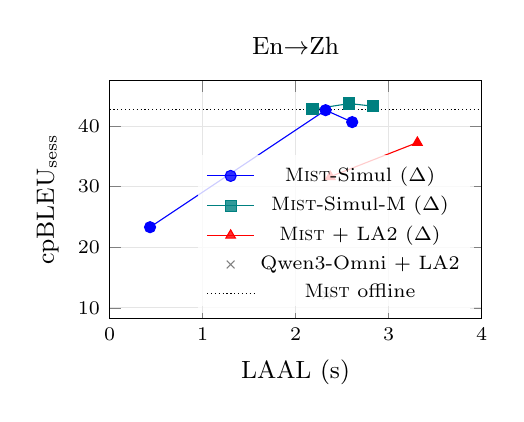
\begin{tikzpicture}\begin{axis}[width=0.52\textwidth, height=4.6cm, xlabel={LAAL (s)}, ylabel={cpBLEU$_\text{sess}$}, title={En$\rightarrow$Zh}, title style={font=\small}, tick label style={font=\scriptsize}, label style={font=\small}, xmin=0, xmax=4, enlarge y limits=0.12, grid=major, grid style={gray!20}, legend style={font=\scriptsize, at={(0.98,0.02)}, anchor=south east, draw=none, fill=white, fill opacity=0.8, text opacity=1}]
\addplot[blue, mark=*] coordinates {(0.435,23.31) (2.323,42.63) (2.609,40.66)}; \addlegendentry{\sys{}-Simul ($\Delta$)}
\addplot[teal, mark=square*] coordinates {(2.183,42.79) (2.579,43.72) (2.832,43.29)}; \addlegendentry{\sys{}-Simul-M ($\Delta$)}
\addplot[red, mark=triangle*] coordinates {(2.373,31.64) (3.310,37.29)}; \addlegendentry{\sys{} + LA2 ($\Delta$)}
\addplot[gray, only marks, mark=x] coordinates {(2.333,12.07)}; \addlegendentry{Qwen3-Omni + LA2}
\addplot[black, densely dotted, domain=0:4, samples=2] {42.81}; \addlegendentry{\sys{} offline}
\end{axis}\end{tikzpicture}
\hfill
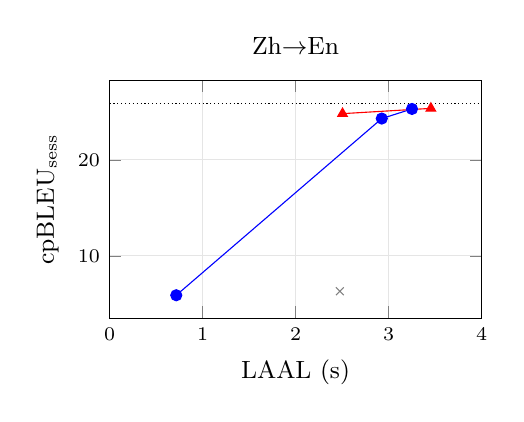
\begin{tikzpicture}\begin{axis}[width=0.52\textwidth, height=4.6cm, xlabel={LAAL (s)}, ylabel={cpBLEU$_\text{sess}$}, title={Zh$\rightarrow$En}, title style={font=\small}, tick label style={font=\scriptsize}, label style={font=\small}, xmin=0, xmax=4, enlarge y limits=0.12, grid=major, grid style={gray!20}]
\addplot[blue, mark=*] coordinates {(0.717,5.89) (2.927,24.30) (3.252,25.30)};
\addplot[red, mark=triangle*] coordinates {(2.505,24.81) (3.455,25.36)};
\addplot[gray, only marks, mark=x] coordinates {(2.476,6.31)};
\addplot[black, densely dotted, domain=0:4, samples=2] {25.86};
\end{axis}\end{tikzpicture}
\caption{Latency--quality trade-off (text) over the read interval $\Delta\in\{0.5,1,2\}$\,s (left to right).
\sys{}-Simul is trained at $\Delta=1$\,s, \sys{}-Simul-M at mixed intervals (En$\rightarrow$Zh). The dotted line is the offline \sys{}. Numbers in Table~\ref{tab:tradeoff}.}
\label{fig:tradeoff}
\end{figure*}

\begin{table}[t]
\centering\small
\setlength{\tabcolsep}{2.6pt}
\resizebox{\columnwidth}{!}{\begin{tabular}{lccccc}
\toprule
System & LAAL\,s & cpBLEU$_\text{sess}$ & BLEU$_\text{blind}$ & Spk & DER \\
\midrule
Cascade, same-data translator & -- & 15.25 & 15.58 & 92.5 & 13.1 \\
Cascade, turn-trained translator & -- & 13.05 & 13.11 & 76.4 & 26.0 \\
\sys{} w/o speaker stream & -- & 8.34 & 16.38 & 87.1 & 52.0 \\
\quad + diarizer relabelling & -- & 15.99 & 16.38 & 86.8 & 12.9 \\
\sys{} (offline) & -- & 14.90 & 15.11 & 91.9 & 14.7 \\
\midrule
\sys{} (offline) + LA2 & 2.84 & 12.10 & 12.55 & 91.7 & 12.9 \\
\sys{}-Simul model + LA2 & 3.40 & 13.44 & 13.62 & 91.3 & 10.6 \\
\sys{}-Simul & 3.62 & 11.98$\pm$1.41$^{2}$ & 12.14 & 91.5 & 10.8 \\
\bottomrule
\end{tabular}}
\caption{Real Mandarin meetings (AliMeeting test, Zh$\rightarrow$En, 20 meetings, 4{,}243 reference windows; zero-shot: no AliMeeting data in training). The English references are machine translations of the human transcripts (their automatic quality estimate: Appendix~\ref{app:qe7}).}
\label{tab:real7}
\end{table}

\begin{table}[t]
\centering\small
\setlength{\tabcolsep}{3pt}
\resizebox{\columnwidth}{!}{\begin{tabular}{llccccc}
\toprule
Set & Seed & cpBLEU$_\text{sess}$ & cpBLEU$_\text{win}$ & LAAL\,s & Spk & Empty \\
\midrule
En$\rightarrow$Zh & 1 & 42.63 & 43.06 & 2.32 & 90.6 & 0.0 \\
 & 2 & 43.10 & 43.57 & 2.35 & 90.4 & 0.0 \\
 & 3 & 43.52 & 44.01 & 2.53 & 90.3 & 0.0 \\
 & mean $\pm$ s.d. & 43.08 $\pm$ 0.45 & & 2.40 & & \\
\midrule
Zh$\rightarrow$En & 1 & 24.30 & 25.81 & 2.93 & 93.2 & 0.0 \\
 & 2 & 22.79 & 24.07 & 3.16 & 93.0 & 0.0 \\
 & mean $\pm$ s.d. & 23.55 $\pm$ 1.07 & & 3.04 & & \\
\midrule
AliMeeting & 1 & 12.97 & 13.09 & 3.09 & 91.5 & 0.0 \\
 & 2 & 10.98 & 11.08 & 4.15 & 91.5 & 0.0 \\
 & mean $\pm$ s.d. & 11.98 $\pm$ 1.41 & & 3.62 & & \\
\bottomrule
\end{tabular}}
\caption{\sys{}-Simul per training seed ($\Delta{=}1$\,s, reference windows; AliMeeting uses the Zh$\rightarrow$En models). Seed 1 is the model of v6; seeds 2 and 3 differ only in the random seed (seed 3 of En$\rightarrow$Zh was retrained from scratch, prereg\_v7 amendment 6). Empty: windows with no output (failures).}
\label{tab:seeds7}
\end{table}


\paragraph{Read interval.} Varying $\Delta$ at test time (Figure~\ref{fig:tradeoff}): at 2\,s, \sys{}-Simul loses
\num{cost:en2zh:d2} points for \num{lat:en2zh:d2}\,s more LAAL (LocalAgreement trails by \num{gain:en2zh:simul2}); at
0.5\,s, earlier than any training read, it commits guesses and collapses (\num{tx:en2zh:S2dl_d0.5:cp};
Zh$\rightarrow$En \num{tx:zh2en:S2dl_d0.5:cp}). Drawing the
interval per training window from $\{0.5,1,2\}$\,s (\sys{}-Simul-M) removes the collapse: \num{tx:en2zh:S2dlm_d0.5:cp}
at 0.5\,s with \num{tx:en2zh:S2dlm_d0.5:laal}\,s LAAL, by waiting longer, not by sub-second commits.


\begin{table*}[t]
\centering\small
\setlength{\tabcolsep}{4pt}
\resizebox{\textwidth}{!}{\begin{tabular}{lccccc@{\hskip 10pt}ccccc}
\toprule
 & \multicolumn{5}{c}{En$\rightarrow$Zh} & \multicolumn{5}{c}{Zh$\rightarrow$En} \\
\cmidrule(lr){2-6}\cmidrule(lr){7-11}
System & LAAL & First & cpBLEU$_\text{sess}$ & BLEU$_\text{blind}$ & Len & LAAL & First & cpBLEU$_\text{sess}$ & BLEU$_\text{blind}$ & Len \\
\midrule
Qwen3-Omni + LA2, $\Delta{=}1$\,s & 2.33 & 1.85 & 12.07 & 26.87 & 0.75 & 2.48 & 2.08 & 6.31 & 14.11 & 0.78 \\
\sys{} (offline) + LA2, $\Delta{=}1$\,s & 2.37 & 2.23 & 31.64 & 32.74 & 1.18 & 2.50 & 2.24 & 24.81 & 27.67 & 0.94 \\
\sys{} (offline) + LA2, $\Delta{=}2$\,s & 3.31 & 2.98 & 37.29 & 38.33 & 1.06 & 3.46 & 2.98 & 25.36 & 28.21 & 0.94 \\
\sys{}-Simul, $\Delta{=}0.5$\,s & 0.43 & 0.25 & 23.31 & 24.30 & 1.27 & 0.72 & 0.24 & 5.89 & 10.79 & 1.34 \\
\sys{}-Simul, $\Delta{=}1$\,s & 2.32 & 2.19 & 42.63 & 42.80 & 0.99 & 2.93 & 2.79 & 24.30 & 26.71 & 1.03 \\
\sys{}-Simul, $\Delta{=}2$\,s & 2.61 & 2.43 & 40.66 & 40.86 & 1.01 & 3.25 & 3.03 & 25.30 & 27.71 & 0.94 \\
\sys{}-Simul-M, $\Delta{=}0.5$\,s & 2.18 & 2.23 & 42.79 & 42.97 & 0.98 & \multicolumn{5}{c}{--} \\
\sys{}-Simul-M, $\Delta{=}1$\,s & 2.58 & 2.45 & 43.72 & 43.78 & 0.97 & \multicolumn{5}{c}{--} \\
\sys{}-Simul-M, $\Delta{=}2$\,s & 2.83 & 2.67 & 43.29 & 43.47 & 0.97 & \multicolumn{5}{c}{--} \\
\sys{}-Simul, 1{,}000 steps & \multicolumn{5}{c}{--} & 2.85 & 2.83 & 24.78 & 27.26 & 0.96 \\
\bottomrule
\end{tabular}}
\caption{Latency and quality of the simultaneous systems at read intervals $\Delta$ (\sys{}-Simul is trained with
reads every 1\,s; \sys{}-Simul-M with reads every 0.5, 1 or 2\,s, drawn per training window, En$\rightarrow$Zh only;
the last row is the 1{,}000-step Zh$\rightarrow$En model of our previous version; Zh$\rightarrow$En at 0.5\,s: 1{,}419 of the 3{,}317 windows were decoded with batch 4 instead of 16 after a memory stop). LAAL and \emph{First} (delay of the first commit after the first
source utterance starts) in seconds. Len: output over reference length (characters for Chinese, words for
English).}
\label{tab:tradeoff}
\end{table*}

\begin{table*}[t]
\centering\small
\resizebox{\textwidth}{!}{\begin{tabular}{lccccccccc}
\toprule
System & cpBLEU$_\text{sess}$ & cpBLEU$_\text{win}$ & cpchrF$_\text{sess}$ & BLEU$_\text{blind}$ & Len & Spk & DER & Conf. & Empty \\
\midrule
Qwen3-Omni, prompted & 12.82 & 26.91 & 12.50 & 29.01 & 0.77 & 65.0 & 67.6 & 46.8 & 0.0 \\
Cascade: diarizer $\rightarrow$ Qwen3-Omni & 29.47 & 29.52 & 25.07 & 29.16 & 0.87 & 88.2 & 25.8 & 0.8 & 0.0 \\
Cascade: diarizer $\rightarrow$ same-data model & 36.29 & 36.36 & 33.90 & 37.01 & 1.11 & 88.2 & 25.8 & 0.8 & 0.0 \\
\sys{} w/o speaker stream & 21.17 & 42.32 & 19.65 & 43.40 & 0.95 & 84.8 & 54.5 & 43.5 & 0.1 \\
\sys{} (offline) & 42.81 & 42.97 & 36.71 & 43.33 & 0.95 & 89.5 & 14.0 & 1.7 & 0.4 \\
\sys{} (offline), oracle stream & 42.32 & 42.58 & 36.27 & 42.95 & 0.95 & 92.2 & 14.2 & 1.3 & 0.3 \\
Qwen3-Omni + LA2 & 12.07 & 25.05 & 11.86 & 26.87 & 0.75 & 65.0 & 101.5 & 0.1 & 0.0 \\
\sys{} (offline) + LA2 & 31.64 & 32.16 & 33.52 & 32.74 & 1.18 & 87.8 & 15.2 & 3.9 & 0.0 \\
\sys{}-Simul & 42.63 & 43.06 & 36.81 & 42.80 & 0.99 & 90.6 & 11.0 & 2.3 & 0.0 \\
\bottomrule
\end{tabular}}
\caption{All text metrics, En$\rightarrow$Zh. cpBLEU$_\text{win}$ matches speakers once per window; Len: output
over reference length (characters); Conf.: speaker-confusion part of
DER; Empty: windows with no output.}
\label{tab:full-en2zh}
\end{table*}

\begin{table*}[t]
\centering\small
\resizebox{\textwidth}{!}{\begin{tabular}{lccccccccc}
\toprule
System & cpBLEU$_\text{sess}$ & cpBLEU$_\text{win}$ & cpchrF$_\text{sess}$ & BLEU$_\text{blind}$ & Len & Spk & DER & Conf. & Empty \\
\midrule
Qwen3-Omni, prompted & 6.40 & 13.55 & 19.00 & 14.24 & 0.76 & 63.5 & 78.7 & 50.6 & 0.0 \\
Cascade: diarizer $\rightarrow$ Qwen3-Omni & 16.07 & 16.67 & 40.61 & 16.84 & 0.94 & 83.6 & 15.5 & 4.1 & 0.0 \\
Cascade: diarizer $\rightarrow$ same-data model & 22.36 & 23.22 & 48.18 & 24.85 & 1.04 & 83.6 & 15.5 & 4.1 & 0.0 \\
\sys{} w/o speaker stream & 12.20 & 26.24 & 26.17 & 28.13 & 0.91 & 84.9 & 57.4 & 48.5 & 0.1 \\
\sys{} (offline) & 25.86 & 27.06 & 49.06 & 28.43 & 0.91 & 91.3 & 16.0 & 5.4 & 0.0 \\
\sys{} (offline), oracle stream & 27.32 & 27.39 & 51.29 & 28.37 & 0.92 & 95.9 & 11.6 & 1.2 & 0.1 \\
Qwen3-Omni + LA2 & 6.31 & 13.41 & 18.74 & 14.11 & 0.78 & 63.5 & 101.6 & 0.1 & 0.0 \\
\sys{} (offline) + LA2 & 24.81 & 26.23 & 47.98 & 27.67 & 0.94 & 90.7 & 17.3 & 6.6 & 0.0 \\
\sys{}-Simul & 24.30 & 25.81 & 47.72 & 26.71 & 1.03 & 93.2 & 12.8 & 6.3 & 0.0 \\
\bottomrule
\end{tabular}}
\caption{All text metrics, Zh$\rightarrow$En. cpBLEU$_\text{win}$ matches speakers once per window; Len: output
over reference length (words); Conf.: speaker-confusion part of
DER; Empty: windows with no output.}
\label{tab:full-zh2en}
\end{table*}


\section{Statistics}
\label{app:sig}
\label{app:stats7}

\begin{table*}[t]
\centering\small
\setlength{\tabcolsep}{3.5pt}
\resizebox{\textwidth}{!}{\begin{tabular}{llrrrrrrl}
\toprule
Test & Comparison & Mtgs & $\Delta$ & 95\% CI & + decoder noise & $p_\text{perm}$ & $p_\text{Holm}$ & verdict \\
\midrule
E-on1 & En$\rightarrow$Zh whole meetings, \sys{}-Simul vs.\ \sys{} + LA2 (tcpBLEU) & 16 & 5.83 & [3.09, 8.48] & [3.17, 8.48] & {<}0.001 & {<}0.001 & a better \\
E-on2 & Zh$\rightarrow$En whole meetings, same & 16 & 0.59 & [$-$1.00, 1.15] & [$-$0.56, 1.75] & 0.079 & 0.238 & tie \\
E-on3 & AliMeeting whole meetings, same & 20 & 0.38 & [$-$1.55, 2.19] & [$-$1.52, 2.28] & 0.711 & 0.951 & tie \\
E-cas1 & En$\rightarrow$Zh, \sys{} vs.\ turn-trained cascade (cpBLEU$_\text{sess}$) & 16 & 7.54 & [4.86, 10.47] & [4.70, 10.38] & {<}0.001 & {<}0.001 & a better \\
E-cas2 & Zh$\rightarrow$En, same & 16 & 2.17 & [1.65, 2.81] & [1.44, 2.90] & {<}0.001 & {<}0.001 & a better \\
E-cas3 & AliMeeting, same & 20 & 1.85 & [1.14, 2.63] & [1.03, 2.67] & {<}0.001 & 0.001 & a better \\
E-seed-en & En$\rightarrow$Zh, \sys{}-Simul (seed mean) vs.\ \sys{} + LA2 & 16 & 11.44 & [4.45, 17.22] & [5.09, 17.79] & {<}0.001 & 0.003 & a better \\
E-seed-zh & Zh$\rightarrow$En, same & 16 & $-$1.27 & [$-$4.75, 0.73] & [$-$4.22, 1.69] & 0.475 & 0.951 & tie \\
\bottomrule
\end{tabular}}
\caption{The eight pre-registered tests of v7 (prereg\_v7). $\Delta$: first minus second system; 95\% CI: cluster bootstrap over meetings; + decoder noise: the same interval widened by the run-to-run noise of decoding (Appendix~\ref{app:stats7}); $p_\text{perm}$: exact two-sided permutation test over meeting sign flips; $p_\text{Holm}$: Holm-adjusted over the eight. A difference is called real only if $p_\text{Holm}<0.05$ and the widened interval excludes 0; otherwise ``tie''.}
\label{tab:reg7}
\end{table*}

\begin{table*}[t]
\centering\footnotesize
\setlength{\tabcolsep}{3pt}
\resizebox{\textwidth}{!}{\begin{tabular}{llrrrrrl}
\toprule
Set & Comparison & Mtgs & $\Delta$ & 95\% CI & + decoder noise & $p_\text{perm}$ & verdict \\
\midrule
En$\rightarrow$Zh & \sys{} vs.\ same-data casc. & 16 & 6.52 & [5.47, 7.59] & [5.36, 7.68] & {<}0.001 & a better \\
En$\rightarrow$Zh & \sys{} vs.\ relabelling & 16 & 0.75 & [0.13, 1.31] & [$-$0.02, 1.52] & 0.036 & tie \\
En$\rightarrow$Zh & \sys{}-Simul vs.\ \sys{}+LA2 & 16 & 10.98 & [3.87, 16.73] & [4.53, 17.44] & 0.006 & a better \\
En$\rightarrow$Zh (speech) & \sys{} vs.\ same-data casc. & 16 & 1.63 & [0.26, 2.90] & [0.23, 3.04] & 0.048 & a better \\
En$\rightarrow$Zh (speech) & \sys{}-Simul vs.\ \sys{}+LA2 & 16 & 2.10 & [1.47, 2.69] & [1.31, 2.89] & {<}0.001 & a better \\
Zh$\rightarrow$En & \sys{} vs.\ same-data casc. & 16 & 3.50 & [2.68, 4.36] & [2.54, 4.46] & {<}0.001 & a better \\
Zh$\rightarrow$En & \sys{} vs.\ relabelling & 16 & 1.20 & [0.81, 1.56] & [0.64, 1.75] & {<}0.001 & a better \\
Zh$\rightarrow$En & \sys{}-Simul vs.\ \sys{}+LA2 & 16 & $-$0.52 & [$-$2.70, 0.66] & [$-$2.45, 1.41] & 0.535 & tie \\
Zh$\rightarrow$En (speech) & \sys{} vs.\ same-data casc. & 16 & 1.97 & [0.59, 3.49] & [0.49, 3.45] & 0.014 & a better \\
Zh$\rightarrow$En (speech) & \sys{}-Simul vs.\ \sys{}+LA2 & 16 & 2.00 & [$-$0.30, 4.78] & [$-$0.52, 4.52] & 0.154 & tie \\
AliMeeting & \sys{} vs.\ same-data casc. & 20 & $-$0.35 & [$-$1.78, 1.08] & [$-$1.85, 1.14] & 0.458 & tie \\
AliMeeting & \sys{} vs.\ relabelling & 20 & $-$1.09 & [$-$1.54, $-$0.68] & [$-$1.67, $-$0.52] & {<}0.001 & b better \\
AliMeeting & \sys{}-Simul vs.\ \sys{}+LA2 & 20 & 0.87 & [$-$0.54, 2.07] & [$-$0.51, 2.25] & 0.276 & tie \\
AliMeeting (speech) & \sys{} vs.\ same-data casc. & 20 & $-$0.75 & [$-$2.12, 0.49] & [$-$2.15, 0.65] & 0.115 & tie \\
AliMeeting (speech) & \sys{}-Simul vs.\ \sys{}+LA2 & 20 & 1.21 & [$-$0.22, 2.20] & [$-$0.08, 2.50] & 0.106 & tie \\
En$\rightarrow$Zh & \sys{} vs.\ turn-trained casc. & 16 & 7.54 & [4.86, 10.47] & [4.70, 10.38] & {<}0.001 & a better \\
En$\rightarrow$Zh & turn-trained casc. vs.\ same-data casc. & 16 & $-$1.02 & [$-$3.72, 1.64] & [$-$3.74, 1.70] & 0.304 & tie \\
En$\rightarrow$Zh & \sys{} vs.\ ref.-turn casc. & 16 & 5.38 & [4.27, 6.42] & [4.17, 6.60] & {<}0.001 & a better \\
En$\rightarrow$Zh & \sys{} vs.\ context casc. & 16 & 19.06 & [18.11, 19.78] & [18.10, 20.01] & {<}0.001 & a better \\
Zh$\rightarrow$En & \sys{} vs.\ turn-trained casc. & 16 & 2.17 & [1.65, 2.81] & [1.44, 2.90] & {<}0.001 & a better \\
Zh$\rightarrow$En & turn-trained casc. vs.\ same-data casc. & 16 & 1.33 & [0.15, 2.46] & [0.08, 2.57] & 0.003 & a better \\
Zh$\rightarrow$En & \sys{} vs.\ ref.-turn casc. & 16 & 0.91 & [$-$0.22, 1.98] & [$-$0.29, 2.12] & 0.208 & tie \\
Zh$\rightarrow$En & \sys{} vs.\ context casc. & 16 & 8.98 & [7.93, 10.01] & [7.88, 10.08] & {<}0.001 & a better \\
AliMeeting & \sys{} vs.\ turn-trained casc. & 20 & 1.85 & [1.14, 2.63] & [1.03, 2.67] & {<}0.001 & a better \\
AliMeeting & turn-trained casc. vs.\ same-data casc. & 20 & $-$2.20 & [$-$3.81, $-$0.50] & [$-$3.97, $-$0.44] & 0.004 & b better \\
En$\rightarrow$Zh & \sys{}-Simul vs.\ stream. casc. & 16 & 7.47 & [5.57, 9.37] & [5.50, 9.44] & {<}0.001 & a better \\
En$\rightarrow$Zh & \sys{}-Simul vs.\ Simul model+LA2 & 16 & 3.42 & [0.14, 8.08] & [$-$0.88, 7.72] & 0.134 & tie \\
En$\rightarrow$Zh & Simul model+LA2 vs.\ \sys{}+LA2 & 16 & 7.57 & [1.72, 13.57] & [1.55, 13.58] & 0.039 & a better \\
En$\rightarrow$Zh & \sys{}-Simul vs.\ fixed lag 1\,s & 8 & 23.29 & [20.78, 25.38] & [20.84, 25.73] & 0.008 & a better \\
En$\rightarrow$Zh & \sys{}-Simul vs.\ fixed lag 2\,s & 8 & $-$0.75 & [$-$2.91, 0.63] & [$-$2.78, 1.28] & 0.148 & tie \\
En$\rightarrow$Zh & fixed lag 2\,s vs.\ \sys{}+LA2 & 8 & 15.35 & [3.36, 21.89] & [5.85, 24.86] & 0.008 & a better \\
Zh$\rightarrow$En & \sys{}-Simul vs.\ stream. casc. & 16 & 2.74 & [0.54, 4.19] & [0.88, 4.61] & 0.010 & a better \\
Zh$\rightarrow$En & \sys{}-Simul vs.\ Simul model+LA2 & 16 & $-$0.56 & [$-$2.74, 0.55] & [$-$2.41, 1.29] & 0.594 & tie \\
Zh$\rightarrow$En & Simul model+LA2 vs.\ \sys{}+LA2 & 16 & 0.04 & [$-$0.32, 0.45] & [$-$0.53, 0.62] & 0.825 & tie \\
AliMeeting & \sys{}-Simul vs.\ Simul model+LA2 & 20 & $-$0.47 & [$-$1.74, 0.49] & [$-$1.75, 0.81] & 0.548 & tie \\
AliMeeting & Simul model+LA2 vs.\ \sys{}+LA2 & 20 & 1.34 & [$-$0.31, 2.44] & [$-$0.08, 2.76] & 0.089 & tie \\
En$\rightarrow$Zh whole mtgs & sp2\_on\_S2dl vs.\ sp2\_on\_O2\_LA2 & 16 & 1.58 & [1.15, 1.97] & [1.00, 2.16] & {<}0.001 & a better \\
Zh$\rightarrow$En whole mtgs & sp2\_on\_S2dl vs.\ sp2\_on\_O2\_LA2 & 16 & 1.69 & [0.02, 3.47] & [$-$0.15, 3.53] & 0.096 & tie \\
AliMeeting whole mtgs & sp2\_on\_S2dl vs.\ sp2\_on\_O2\_LA2 & 20 & 0.29 & [$-$1.03, 1.48] & [$-$1.02, 1.61] & 0.671 & tie \\
\bottomrule
\end{tabular}}
\caption{Exploratory comparisons of v7 (cpBLEU$_\text{sess}$ on reference windows, ASR-cpBLEU for speech, tcpBLEU for whole meetings), on the windows both systems decoded. Columns as Table~\ref{tab:reg7}; no multiple-test correction (exploratory). Fixed lag is on the 8-meeting subset (prereg\_v7 amendment 2).}
\label{tab:sig7}
\end{table*}


Every comparison uses one procedure. The difference A$-$B is taken over the windows both systems decoded. Its 95\%
interval comes from 1{,}000 bootstrap resamples of whole meetings (16 AMI, 20 AliMeeting); the slot-to-speaker matching
is made per meeting, so a meeting resample re-uses exactly the matching a re-match would find. The $p$ value is an
exact two-sided permutation test that flips the two systems' outputs per meeting over all $2^{16}$ (AMI) or $2^{20}$
(AliMeeting) assignments, so it cannot go below $2^{-15}\approx3\cdot10^{-5}$ or $2^{-19}$. Leave-one-meeting-out
minima and maxima and the per-meeting differences are in the released statistics file. Seed comparisons average the
difference over the training seeds; their bootstrap resamples meetings and seeds, their permutation flips a meeting's
outputs for all seeds at once. The decoder adds noise that neither test contains: greedy bf16 decoding of the MoE Thinker
is not batch-invariant (Appendix~\ref{app:noise}), so we widen the meeting interval by
$\sigma_\text{dec}(n)=\sigma_0/\sqrt{n}$ for $n$ scored windows (variances added), with $\sigma_0$ the larger of the v6
estimate (12.3) and the v7 re-decode (\num{v7:nchk:diff} tcpBLEU on 1{,}412 windows). A difference is called real only if
$p<0.05$ (Holm-adjusted over the eight pre-registered tests of Table~\ref{tab:reg7}) and the widened interval excludes
0. Table~\ref{tab:sig7} lists the exploratory comparisons without correction.

\section{Single- and Multi-Speaker Windows, Errors}
\label{app:more}

\begin{table}[t]
\centering\small
\resizebox{\columnwidth}{!}{\begin{tabular}{lccccc}
\toprule
 & \multicolumn{2}{c}{cpBLEU$_\text{sess}$} & \multicolumn{2}{c}{DER} & Spk-count \\
System & single & multi & single & multi & multi \\
\midrule
\multicolumn{6}{l}{\emph{En$\rightarrow$Zh}} \\
Qwen3-Omni, prompted & 16.64 & 9.97 & 68.0 & 65.4 & 0.0 \\
Cascade: diarizer $\rightarrow$ same-data model & 43.21 & 31.97 & 22.1 & 28.6 & 78.7 \\
\sys{} w/o speaker stream & 25.04 & 18.28 & 48.1 & 57.7 & 57.6 \\
\sys{} (offline) & 47.42 & 39.39 & 6.9 & 19.6 & 72.8 \\
\sys{} (offline), oracle stream & 47.59 & 38.40 & 6.2 & 20.5 & 80.1 \\
\sys{} (offline) + LA2 & 43.75 & 25.42 & 8.4 & 20.5 & 68.1 \\
\sys{}-Simul & 45.79 & 40.21 & 5.4 & 15.4 & 77.0 \\
\multicolumn{6}{l}{\emph{Zh$\rightarrow$En}} \\
Qwen3-Omni, prompted & 9.26 & 4.49 & 79.6 & 75.1 & 0.0 \\
Cascade: diarizer $\rightarrow$ same-data model & 27.71 & 19.34 & 13.5 & 16.9 & 74.2 \\
\sys{} w/o speaker stream & 15.68 & 9.94 & 50.0 & 60.9 & 59.6 \\
\sys{} (offline) & 29.09 & 23.76 & 9.9 & 20.3 & 77.7 \\
\sys{} (offline), oracle stream & 30.64 & 25.16 & 4.9 & 16.4 & 88.8 \\
\sys{} (offline) + LA2 & 27.07 & 23.36 & 13.2 & 20.2 & 75.6 \\
\sys{}-Simul & 27.61 & 21.64 & 10.2 & 14.6 & 82.3 \\
\bottomrule
\end{tabular}}
\caption{Single- and multi-speaker test windows.}
\label{tab:groups}
\end{table}

\begin{table}[t]
\centering\small
\setlength{\tabcolsep}{3pt}
\resizebox{\columnwidth}{!}{\begin{tabular}{lcccc}
\toprule
System & cpBLEU$_\text{sess}$ & BLEU$_\text{blind}$ & Spk-count & DER \\
\midrule
Qwen3-Omni, prompted & 14.85 & 29.34 & 61.2 & 63.4 \\
Cascade: diarizer $\rightarrow$ same-data model & 37.53 & 37.91 & 86.3 & 20.7 \\
\sys{} w/o speaker stream & 21.57 & 43.91 & 83.8 & 55.4 \\
\sys{} (offline) & 43.36 & 43.83 & 89.4 & 15.5 \\
\bottomrule
\end{tabular}}
\caption{En$\rightarrow$Zh test windows opened and closed by the diarizer itself (871
windows that contain whole utterances), offline.}
\label{tab:diar}
\end{table}

\begin{table}[t]
\centering\small
\setlength{\tabcolsep}{2.4pt}
\resizebox{\columnwidth}{!}{\begin{tabular}{lcccccc}
\toprule
System & Under & Over & Wrong & Omit & Insert & Start\,s \\
\midrule
\multicolumn{7}{l}{\emph{En$\rightarrow$Zh}} \\
\sys{} w/o speaker stream & 41.2 & 1.2 & 77.4 & 2.4 & 0.9 & 0.42 \\
\sys{} (offline) & 25.9 & 1.3 & 10.9 & 2.6 & 4.2 & 0.42 \\
\sys{} (offline), oracle stream & 19.1 & 0.7 & 11.7 & 4.4 & 3.9 & 0.42 \\
\sys{} (offline) + LA2 & 29.6 & 2.3 & 13.5 & 1.6 & 3.8 & 0.48 \\
\sys{}-Simul & 21.1 & 1.9 & 14.3 & 0.3 & 5.9 & 0.82 \\
\multicolumn{7}{l}{\emph{Zh$\rightarrow$En}} \\
\sys{} w/o speaker stream & 38.9 & 1.5 & 71.0 & 1.2 & 1.5 & 0.26 \\
\sys{} (offline) & 18.2 & 4.1 & 17.2 & 1.6 & 3.3 & 0.28 \\
\sys{} (offline), oracle stream & 11.2 & 0.0 & 11.1 & 1.2 & 2.9 & 0.28 \\
\sys{} (offline) + LA2 & 19.8 & 4.6 & 17.9 & 1.1 & 3.8 & 0.29 \\
\sys{}-Simul & 14.5 & 3.1 & 17.4 & 0.2 & 6.1 & 0.42 \\
\bottomrule
\end{tabular}}
\caption{Errors on the multi-speaker test windows (\%). \emph{Under}/\emph{Over}: windows with too few / too many
speakers; \emph{Wrong}: segments whose speaker differs from that of the reference utterance they align to;
\emph{Omit}: reference utterances no segment aligns to; \emph{Insert}: segments aligned to no reference; \emph{Start}:
mean start-time error (s), per committed chunk for the simultaneous systems. Slots are those the targets were built
with (offline or low-latency preset). Without the speaker stream, \emph{Wrong} is measured against slots the model never sees.}
\label{tab:errors}
\end{table}


\paragraph{Remaining errors.} Most remaining errors are short back-channels (``yeah'', ``okay'') of a second speaker in
overlap that are merged into the main turn or dropped: \num{er:en2zh:O2:under}\% of the multi-speaker En$\rightarrow$Zh
windows are under-counted (\num{er:en2zh:O2-nosd:under}\% without the speaker stream), while whole utterances are
rarely omitted (\num{er:en2zh:O2:omit}\%; Appendix~\ref{app:more}).

\sys{} loses \num{tx:en2zh:O2:single} $\rightarrow$ \num{tx:en2zh:O2:multi} cpBLEU$_\text{sess}$ from single- to
multi-speaker windows (En$\rightarrow$Zh) and finds the right number of speakers in only \num{tx:en2zh:O2:spkmulti}\% of
the latter. Table~\ref{tab:groups} splits the test set by the number of speakers, Table~\ref{tab:errors} counts the errors on
multi-speaker windows after aligning each output segment to a reference utterance by time overlap and text
similarity, and Table~\ref{tab:diar} evaluates on windows cut by the diarizer.

\section{Example}
\label{app:example}

Table~\ref{tab:example} shows a window in which speaker B says ``yes'' while A is still talking. The cascade translates
the overlapped stretch in every turn that contains it: ``yes'' appears in A's turn, in a spurious third slot and in B's
turn. \sys{} writes it once and attributes it to B.

\begin{table*}[t]
\centering\small
\begin{tabular}{lp{0.78\textwidth}}
\toprule
English source & \textbf{A} [0.3--4.3\,s] uh so this is these are the circuits un underneath the buttons \textbf{A} [4.3--6.9\,s] uh can you see the black uh round marks \textbf{A} [6.9--8.1\,s] they they are the circuits \textbf{B} [6.9--7.2\,s] yes \\
Reference & \textbf{A} [0.3] \zh{呃\hspace{0pt}，\hspace{0pt}这\hspace{0pt}些\hspace{0pt}就\hspace{0pt}是\hspace{0pt}按\hspace{0pt}钮\hspace{0pt}下\hspace{0pt}面\hspace{0pt}的\hspace{0pt}电\hspace{0pt}路\hspace{0pt}。} \textbf{A} [4.3] \zh{呃\hspace{0pt}，\hspace{0pt}你\hspace{0pt}能\hspace{0pt}看\hspace{0pt}到\hspace{0pt}那\hspace{0pt}些\hspace{0pt}黑\hspace{0pt}色\hspace{0pt}的\hspace{0pt}圆\hspace{0pt}形\hspace{0pt}标\hspace{0pt}记\hspace{0pt}吗\hspace{0pt}？} \textbf{A} [6.9] \zh{它\hspace{0pt}们\hspace{0pt}就\hspace{0pt}是\hspace{0pt}电\hspace{0pt}路} \textbf{B} [6.9] \zh{是\hspace{0pt}的} \\
\midrule
Cascade (same data) & \textbf{A} [0.2] \zh{呃\hspace{0pt}，\hspace{0pt}这\hspace{0pt}些\hspace{0pt}就\hspace{0pt}是\hspace{0pt}按\hspace{0pt}钮\hspace{0pt}下\hspace{0pt}面\hspace{0pt}的\hspace{0pt}电\hspace{0pt}路\hspace{0pt}。} \textbf{A} [4.3] \zh{呃\hspace{0pt}，\hspace{0pt}你\hspace{0pt}能\hspace{0pt}看\hspace{0pt}到\hspace{0pt}那\hspace{0pt}些\hspace{0pt}黑\hspace{0pt}色\hspace{0pt}的\hspace{0pt}圆\hspace{0pt}形\hspace{0pt}标\hspace{0pt}记\hspace{0pt}吗\hspace{0pt}？\hspace{0pt}它\hspace{0pt}们\hspace{0pt}就\hspace{0pt}是\hspace{0pt}电\hspace{0pt}路\hspace{0pt}。\hspace{0pt}是\hspace{0pt}的} \textbf{?} [6.6] \zh{是\hspace{0pt}的} \textbf{B} [6.9] \zh{是\hspace{0pt}的} \\
\sys{} (offline) & \textbf{A} [0.3] \zh{呃\hspace{0pt}，\hspace{0pt}这\hspace{0pt}些\hspace{0pt}就\hspace{0pt}是\hspace{0pt}按\hspace{0pt}钮\hspace{0pt}下\hspace{0pt}方\hspace{0pt}的\hspace{0pt}电\hspace{0pt}路\hspace{0pt}。} \textbf{A} [4.4] \zh{呃\hspace{0pt}，\hspace{0pt}你\hspace{0pt}能\hspace{0pt}看\hspace{0pt}到\hspace{0pt}那\hspace{0pt}些\hspace{0pt}黑\hspace{0pt}色\hspace{0pt}的\hspace{0pt}圆\hspace{0pt}形\hspace{0pt}标\hspace{0pt}记\hspace{0pt}吗\hspace{0pt}？\hspace{0pt}它\hspace{0pt}们\hspace{0pt}就\hspace{0pt}是\hspace{0pt}电\hspace{0pt}路\hspace{0pt}。} \textbf{B} [7.0] \zh{是\hspace{0pt}的} \\
\bottomrule
\end{tabular}
\caption{Test window \texttt{IS1009c\_0126} with overlapping speech. Speakers are lettered by first appearance in the reference; output speakers are mapped to reference speakers by the meeting-level matching of cpBLEU$_\text{sess}$ (``?'' = unmatched). Times in seconds from the window start.}
\label{tab:example}
\end{table*}


\section{Chinese AMI Meetings}
\label{app:zhdata}

\paragraph{Construction.} The Chinese meetings reuse the En$\rightarrow$Zh translations of every AMI utterance. A first
version laid the MT pipeline's own Chinese speech (one voice clone per utterance) on the meeting clock; the audit below
found that the diarizer split most speakers into several slots, because a person sounded different from one utterance
to the next. We therefore re-spoke every utterance with the UniSS Talker and one voice prompt per speaker. Each clip is
trimmed of leading and trailing silence, set to its speaker's median loudness in the English recording (gain at most
$4\times$, peak below 0.9), placed at the utterance's original start, and sped up or slowed down (pitch kept) towards the
English duration within $[0.8, 1.5]$; a speaker's next clip waits until the previous one ends. The meeting's background
is the quieter half of its speech-free English frames.

\paragraph{Audit.} Table~\ref{tab:zhaudit} lists the checks, the problems they found and the fixes; every check was rerun
after its fix. An utterance that fails the clip checks is left out of the meeting (neither heard nor translated) rather
than dropping its window, which would remove most multi-speaker windows, since the failures are mostly short
back-channels.

\begin{table}[h]
\centering\small
\setlength{\tabcolsep}{3pt}
\resizebox{\columnwidth}{!}{\begin{tabular}{p{2.3cm}p{3.1cm}p{2.6cm}}
\toprule
Check & Problem found & Fix \\
\midrule
Overlap vs.\ English ($\pm$20\%) & +36\% (Chinese longer) & speed-up $\le1.5\times$ \\
 & $-25\%$ after re-speaking & slow-down $\le1.25\times$: $-12$ to $-17\%$ \\
Windows & clock shifts split groups & English utterance groups \\
Intelligibility (CER $\le0.3$) & 17\% fail Whisper & Paraformer recheck; failing clips left out \\
Clipping & bursts in background & quieter frames only, gain cap \\
Diarizer (DER $\le$ English + 10) & 40--44\% vs.\ 28\%, extra slots & one voice per speaker: 17.7--21.7\% \\
 & 13 meetings still fail & meetings dropped (none in test) \\
\bottomrule
\end{tabular}}
\caption{Audit of the Chinese AMI meetings. Left out in the end: 19{,}081 of 123{,}353 utterances (CER 13{,}681; no
translation 5{,}295; long pauses 98; other 7).}
\label{tab:zhaudit}
\end{table}

\section{Read Targets}
\label{app:labels}

\begin{table}[t]
\centering\small
\setlength{\tabcolsep}{3pt}
\resizebox{\columnwidth}{!}{\begin{tabular}{lccccc}
\toprule
 & LAAL & cpBLEU$_\text{sess}$ & Units/blk & 1-unit\,\% & Mid\,\% \\
\midrule
\multicolumn{6}{l}{\emph{En$\rightarrow$Zh}} \\
Deadline labels (\sys{}-Simul) & 2.32 & 42.63 & 6.0 & 11.1 & 12.9 \\
Stable-prefix labels & 2.43 & 32.73 & 8.3 & 8.2 & 36.9 \\
\multicolumn{6}{l}{\emph{Zh$\rightarrow$En}} \\
Deadline labels (\sys{}-Simul) & 2.93 & 24.30 & 5.3 & 36.9 & 0.6 \\
Stable-prefix labels & 2.35 & 24.07 & 4.2 & 32.8 & 32.3 \\
\bottomrule
\end{tabular}}
\caption{Read targets at $\Delta=1$\,s, both continued from the same offline model for 3{,}000 steps. Stable-prefix
labels: at each read, the prefix of the model's own draft that it also writes after hearing the whole window, decoded
with the same plain wait rule. Units/blk: mean characters (Zh) or words (En) per committed block; 1-unit: blocks of a
single unit; Mid: blocks that stop mid-phrase before the same speaker's next block.}
\label{tab:ablation}
\end{table}


Deadline targets (\S\ref{sec:method-simul}) are derived from the reference and its timing. An alternative that needs
neither is to label each read with the \emph{stable prefix} of the model's own output: the offline model drafts a
continuation from the audio heard so far and another from the whole window, both after the same committed prefix, and
the target is the longest common prefix of the two (speaker and time tokens included), followed by the wait token. We
continued the same offline model for 3{,}000 steps on such reads of 8{,}000 training windows (both directions,
intervals drawn from $\{0.5,1,1,2\}$\,s) and decode it with the same plain wait rule (greedy, the wait token
competing with all others). Table~\ref{tab:ablation} compares
the two at $\Delta=1$\,s: deadline targets are far better in En$\rightarrow$Zh (\num{gain:en2zh:labels} cpBLEU$_\text{sess}$,
$p<0.001$) and slightly better but later in Zh$\rightarrow$En (\num{gain:zh2en:labels}, not significant), so we use them.

\section{Causality of the Speaker Stream}
\label{app:causal}

The streaming runs read posteriors from one low-latency run of the diarizer over the whole session, with every frame
later than $t-\lambda$ zeroed at a read at $t$ (Eq.~\ref{eq:causal}). This equals a causal system only if those frames
do not change when the audio after $t$ is never given. For every test meeting of the three sets we drew three reference
windows and one read time in each (fixed seed), truncated the session audio at that time and ran the diarizer from
scratch with the same model and preset, pooling its 10\,ms output to 80\,ms exactly as for the stream. Over
\num{v6:caus:cuts} cuts and \num{v6:caus:frames} compared frames, the largest absolute difference to the posteriors the
streaming runs read was \num{v6:caus:maxabs} (the fp16 precision in which they are stored), the mean absolute difference \num{v6:caus:mean},
the most active slot agreed on at least \num{v6:caus:arg}\% and the whole set of active slots on at least
\num{v6:caus:slotset}\% of active frames in every cut, and the $>0.5$ decision differed on \num{v6:caus:ndec} frames
(\num{v6:caus:ovldiff} of them among the \num{v6:caus:ovlframes} overlapped frames), every one of them a posterior within
$5\cdot10^{-4}$ of 0.5, i.e.\ an fp16 rounding tie. Our pre-registered criterion (all decisions
identical) is therefore missed by these rounding ties; we consider the stream causal up to floating-point noise and did
not re-decode with prefix posteriors. Prefix runs of the same meeting cut at different times also agree with each other
(\num{v6:caus:selfpairs} pairs, largest difference \num{v6:caus:selfmax}): later audio never changes earlier frames.
(A first comparison script compared the 10\,ms prefix output with the 80\,ms stream and reported large differences; it
was a frame-rate error, corrected before the numbers above.) The audio encoder needs no such test: each read
encodes the audio prefix itself. Algorithm~\ref{alg:read} lists one read.

\begin{figure}[h]
\small
\resizebox{\columnwidth}{!}{\begin{tabular}{@{}l@{}}
\toprule
\textbf{Algorithm 1}: read $r$ of a window that started at $s$ (meeting clock) \\
\midrule
1: $t\gets\min(r\Delta, T)$; audio $\bm{x}_{s:s+t}$ (only what has been heard) \\
2: $\bm{A}\gets\mathrm{Enc}(\bm{x}_{s:s+t})$ \hfill (prefix forward, Eq.~\ref{eq:enc}) \\
3: $\bm{P}^{(r)}\gets$ diarizer frames of $(s, s+t-\lambda]$, later ones zero \hfill (Eq.~\ref{eq:causal}) \\
4: $\bm{E}^{(r)}\gets$ interleave $\bm{A}$ with speaker tokens of $\bm{P}^{(r)}$ \hfill (Eq.~\ref{eq:interleave}) \\
5: greedy decode after the committed tokens until $\wait$ (or $\eos$ if $t=T$) \\
6: commit the new tokens; parse segments; hand each new block to the Talker \\
7: whole meetings: commit time $\gets\max(\text{now},\ \text{window opening known})$; \\
\quad at $t=T$, $\max(\cdot,\ \text{window end known})$ \hfill (\S\ref{sec:method-online}) \\
\quad no slot active $\Rightarrow$ no window; empty decode $\Rightarrow$ nothing spoken \\
\bottomrule
\end{tabular}}
\caption{One read of \sys{}-Simul. The full prompt is re-encoded at every read (no cache is kept across reads).}
\label{alg:read}
\end{figure}

\section{Decoder Run-to-Run Noise}
\label{app:noise}

\paragraph{Batch invariance.} Greedy decoding of the MoE Thinker in bf16 is not invariant to the batch composition:
decoding the same 96 Zh$\rightarrow$En windows at batch 16 and at batch 4 gives token-identical output for only
\num{v6:t13:same}\% of them, with cpBLEU$_\text{sess}$ \num{v6:t13:b16} vs.\ \num{v6:t13:b4}. Differences of this size between
runs decoded in different batches (including the shards re-decoded after a stopped worker, and the late runs that split the
Thinker over two cards, prereg\_v6 amendment 6) are within this noise. To size it for our tests, we resample $N$
windows with replacement from the 96 and take the spread of the difference between the two runs: its standard deviation is
\num{v6:noise:sd1410} cpBLEU at $N{=}1{,}410$ (a whole-meeting subset), \num{v6:noise:sd2375} at 2{,}375 and \num{v6:noise:sd3317}
at 3{,}317. Neither the meeting bootstrap nor the permutation test contains this source: they treat each system's output as
fixed. We therefore widen every interval by it (Appendix~\ref{app:stats7}) and call a difference real only if the widened
interval excludes 0. A second estimate comes from re-decoding the 8 En$\rightarrow$Zh meetings decoded in v6 with the v7
decoder (Appendix~\ref{app:online7}): \num{v7:nchk:diff} tcpBLEU on 1{,}412 windows, smaller than the first; we keep the
larger.

\section{Deadline Targets: How Accurate?}
\label{app:deadline}

For 2{,}000 validation utterances per direction we aligned source and translation with a SimAlign-style
aligner~\citep{jalili2021simalign} (multilingual BERT, layer 8, mutual argmax) and took, for every chunk, the end of the
last source word or character aligned to it or to an earlier chunk, i.e.\ what must have been heard to write it. The
En$\rightarrow$Zh rule (character fraction mapped to AMI word times) deviates from this by \num{v6:dl:en2zh:word_fraction:mae}\,s
on average; \num{v6:dl:en2zh:word_fraction:early}\% of its deadlines precede the evidence, and
\num{v6:dl:en2zh:word_fraction:before}\% do so by more than the 1\,s lag. The Zh$\rightarrow$En duration rule of v5 deviates by
\num{v6:dl:zh2en:duration_v5:mae}\,s (\num{v6:dl:zh2en:duration_v5:early}\% early, \num{v6:dl:zh2en:duration_v5:before}\% by
more than the lag); with forced-aligned character times (FunASR timestamp predictor~\citep{gao2023funasr}) it deviates by
\num{v6:dl:zh2en:char_fraction_v6:mae}\,s (\num{v6:dl:zh2en:char_fraction_v6:early}\% early). Because a window ends 0.3\,s
after its last word and the lag is 1\,s, \num{v6:flush:labels:zh2en}\% of Zh$\rightarrow$En training chunks are due only at
the last read; at test time \sys{}-Simul commits \num{v6:flush:en2zh:S2dl_d1}\% (En$\rightarrow$Zh) and
\num{v6:flush:zh2en:S2dl_d1}\% (Zh$\rightarrow$En) of its output at the last read of a window (LA2 on \sys{}:
\num{v6:flush:en2zh:O2_LA2_d1}\%), which is why the whole-meeting evaluation moves those commits to the moment the end
is known.

\section{Segment-Level Attribution}
\label{app:attr}

\begin{table*}[t]
\centering\small
\setlength{\tabcolsep}{3.5pt}
\resizebox{\textwidth}{!}{\begin{tabular}{llrrrrrrrrr}
\toprule
Set & System & P & R & F1 & Omit & Misattr. & Onset & Offset & Re-entry & $\le$1\,s \\
\midrule
En$\rightarrow$Zh & Prompted & 50.4 & 36.6 & 42.4 & 0.0 & 63.4 & 1.33 & 1.28 & 20.4 & 30.6 \\
 & Cascade, same data & 94.8 & 94.3 & 94.6 & 0.4 & 5.3 & 0.04 & 0.17 & 89.1 & 86.6 \\
 & w/o speaker stream & 56.8 & 51.0 & 53.8 & 1.0 & 48.0 & 0.05 & 0.16 & 40.1 & 43.8 \\
 & \sys{} & 97.5 & 91.1 & 94.2 & 1.2 & 7.8 & 0.05 & 0.18 & 83.3 & 82.1 \\
 & \sys{}-Simul & 94.5 & 87.5 & 90.9 & 0.0 & 12.4 & 0.03 & 0.07 & 76.5 & 68.7 \\
 & \sys{} + LA2 & 91.0 & 85.3 & 88.0 & 0.1 & 14.6 & 0.06 & 0.23 & 75.5 & 65.8 \\
 & \sys{}-Simul-M & 94.7 & 87.4 & 90.9 & 0.0 & 12.6 & 0.03 & 0.07 & 75.5 & 68.7 \\
\midrule
Zh$\rightarrow$En & Cascade, same data & 87.2 & 91.6 & 89.3 & 0.5 & 7.8 & 0.06 & 0.06 & 84.1 & 85.1 \\
 & w/o speaker stream & 54.8 & 49.6 & 52.1 & 0.5 & 49.9 & 0.04 & 0.05 & 41.2 & 45.3 \\
 & \sys{} & 93.5 & 89.6 & 91.5 & 0.4 & 10.0 & 0.03 & 0.06 & 81.6 & 81.9 \\
 & \sys{}-Simul & 90.6 & 86.9 & 88.7 & 0.0 & 13.1 & 0.02 & 0.03 & 75.5 & 74.3 \\
 & \sys{} + LA2 & 89.2 & 85.3 & 87.2 & 0.1 & 14.6 & 0.04 & 0.08 & 70.8 & 70.4 \\
\midrule
AliMeeting & Cascade, same data & 94.1 & 97.9 & 96.0 & 0.1 & 2.0 & 0.10 & 0.12 & 91.4 & 91.8 \\
 & w/o speaker stream & 64.3 & 60.1 & 62.1 & 1.1 & 38.8 & 0.14 & 0.21 & 53.0 & 55.9 \\
 & \sys{} & 96.5 & 93.0 & 94.7 & 2.8 & 4.2 & 0.09 & 0.18 & 83.5 & 83.1 \\
 & \sys{}-Simul & 95.2 & 92.8 & 94.0 & 0.1 & 7.1 & 0.07 & 0.11 & 81.7 & 72.3 \\
 & \sys{} + LA2 & 93.9 & 91.6 & 92.7 & 0.1 & 8.3 & 0.09 & 0.20 & 81.7 & 70.5 \\
\bottomrule
\end{tabular}}
\caption{Segment-level attribution on the test windows. Each reference utterance is checked against the output segments overlapping it (0.5\,s collar): recall (R) = covered by its own speaker after the session matching, Omit = no segment at all, Misattr. = only other speakers' segments; precision (P) = segments that overlap an utterance of their matched speaker. Onset / offset: median error of the nearest segment (s). Re-entry: recall on utterances of a speaker silent for $\ge$60\,s before; $\le$1\,s: recall on utterances of at most one second.}
\label{tab:attr}
\end{table*}


Table~\ref{tab:attr} scores who-said-what-when per reference utterance. The cascades' turns come straight from the
diarizer, so their time placement is as good as or better than \sys{}'s; \sys{}'s gain in cpBLEU is a translation gain on
the same attribution, not better segmentation. Recall on a speaker's first utterance after $\ge$60\,s of silence (re-entry)
stays within a few points of the overall recall for every system that reads the diarizer, and drops by half without
it: identity over the meeting is the diarizer's contribution.

\section{Voice Prompts}
\label{app:voice}

A causal voice prompt ($\ge$1\,s of the slot heard alone before its first commit) exists for
\num{v6:prompt:en2zh:avail}\% (En$\rightarrow$Zh), \num{v6:prompt:zh2en:avail}\% (Zh$\rightarrow$En) and
\num{v6:prompt:ali:avail}\% (AliMeeting) of the output speaker streams of \sys{}-Simul, with
\num{v6:prompt:en2zh:len}\,s of audio on average; during the prompt the strongest other slot has a mean posterior of
\num{v6:prompt:en2zh:other} (En$\rightarrow$Zh) and \num{v6:prompt:zh2en:other} (Zh$\rightarrow$En). The rest
(\num{v6:prompt:en2zh:fallback}\% / \num{v6:prompt:zh2en:fallback}\% / \num{v6:prompt:ali:fallback}\%) fall back to the
window's audio up to the first commit, which may contain other voices. Cold start (re-review M17): from a slot's first activity it takes a median
\num{v8:vp:en2zh:wait}\,s (En$\rightarrow$Zh), \num{v8:vp:zh2en:wait}\,s (Zh$\rightarrow$En) and \num{v8:vp:ali:wait}\,s
(AliMeeting) until 1\,s of it has been heard alone; segments committed earlier use the fallback. Every test meeting has fewer than eight
speakers, so the slots never run out; larger meetings are untested. Voice confusion (Table~\ref{tab:voice}) counts only
output streams of windows with at least two reference speakers; single-speaker windows have no other voice to confuse.

\begin{table*}[t]
\centering\small
\setlength{\tabcolsep}{4pt}
\begin{tabular}{llrrrrrr}
\toprule
 & & \multicolumn{3}{c}{WavLM-SV} & \multicolumn{3}{c}{TitaNet-large} \\
\cmidrule(lr){3-5}\cmidrule(lr){6-8}
Dir. & System & SIM & Confusion [95\% CI] & ID & SIM & Confusion [95\% CI] & ID \\
\midrule
En$\rightarrow$Zh & Cascade, same data & 0.82 & 24.0 [20.7, 27.0] & 62.0 & 0.34 & 9.8 [5.8, 15.9] & 85.9 \\
 & \sys{} & 0.82 & 23.4 [19.2, 27.2] & 62.2 & 0.35 & 10.2 [5.7, 16.3] & 86.7 \\
 & \sys{} + LA2 & 0.83 & 19.8 [17.2, 22.0] & 67.6 & 0.37 & 7.3 [5.4, 9.8] & 90.5 \\
 & \sys{}-Simul & 0.83 & 21.3 [19.6, 23.0] & 66.3 & 0.38 & 6.7 [4.7, 8.8] & 91.9 \\
\midrule
Zh$\rightarrow$En & Cascade, same data & 0.76 & 29.4 [24.3, 35.5] & 55.9 & 0.20 & 24.6 [18.4, 30.4] & 70.7 \\
 & \sys{} & 0.76 & 30.1 [25.5, 35.0] & 56.1 & 0.20 & 25.9 [20.2, 31.0] & 68.8 \\
 & \sys{} + LA2 & 0.77 & 27.1 [23.5, 30.9] & 60.9 & 0.20 & 23.3 [19.4, 27.8] & 71.8 \\
 & \sys{}-Simul & 0.77 & 27.9 [24.5, 31.6] & 60.0 & 0.20 & 23.3 [19.7, 27.4] & 71.4 \\
\bottomrule
\end{tabular}
\caption{Voice of each output speaker's synthesised speech, matched to reference speakers per meeting by the target-language text (v5 matched Zh$\rightarrow$En output against the Chinese source text, which made its Zh$\rightarrow$En matching close to arbitrary; corrected here). SIM: cosine to the attributed speaker's own clean speech. Confusion: share of streams in multi-speaker windows closer to another speaker of the window (interval: meeting bootstrap). ID: the attributed speaker is the closest of all speakers of the meeting. Cosines of the two models are not comparable in scale.}
\label{tab:voice}
\end{table*}


\begin{table}[t]
\centering\small
\setlength{\tabcolsep}{2.5pt}
\resizebox{\columnwidth}{!}{\begin{tabular}{lcccccc}
\toprule
System & cpASR$\uparrow$ & SIM$\uparrow$ & V-conf$\downarrow$ & Misr.$\downarrow$ & UTMOS$\uparrow$ & Abr.$\downarrow$ \\
\midrule
\multicolumn{7}{l}{\emph{En$\rightarrow$Zh}} \\
Prompted & 10.13 & 0.79 & 39.6 & 14.5 & -- & -- \\
Cascade (same data) & 31.06 & 0.82 & 24.0 & 14.7 & 2.76 & -- \\
\sys{} (offline) & 32.69 & 0.82 & 23.4 & 10.7 & 2.77 & -- \\
\sys{} + LA2 & 33.32 & 0.83 & 19.8 & 8.9 & 3.19 & 2.86 \\
\sys{}-Simul & 35.42 & 0.83 & 21.3 & 5.8 & 3.20 & 2.30 \\
\multicolumn{7}{l}{\emph{Zh$\rightarrow$En}} \\
Cascade (same data) & 12.47 & 0.76 & 29.4 & 33.5 & 1.96 & -- \\
\sys{} (offline) & 14.44 & 0.76 & 30.1 & 34.3 & 1.95 & -- \\
\sys{} + LA2 & 15.79 & 0.77 & 27.1 & 23.6 & 1.83 & 1.56 \\
\sys{}-Simul & 17.79 & 0.77 & 27.9 & 18.3 & 1.84 & 0.06 \\
\bottomrule
\end{tabular}}
\caption{Speech of the UniSS Talker: offline systems dubbed, simultaneous ones spoken block by block on one channel with
causal voice prompts. cpASR: cpBLEU$_\text{sess}$ of the ASR transcripts; SIM: WavLM cosine to the attributed speaker
(two speakers of a meeting: 0.75); V-conf: output speakers closer to another speaker of the window
(\%); Misr.: CER of the transcript against the Talker's input (\%); Abr.: abrupt pauses per minute.}
\label{tab:speech}
\end{table}


\section{Pre-registration and Amendments}
\label{app:prereg}

All v7 analyses were registered in \texttt{prereg\_v7} before any v7 decode or score; every change was committed as a
dated amendment before the results it touches: \num{v7:prereg:list}. The registration fixes the full meeting lists
(AMI test EN2002a--d, ES2004a--d, IS1009a--d, TS3003a--d; all 20 AliMeeting test meetings), the eight confirmatory tests
and their Holm family, the decoder-noise widening and the dev gates. The amendments were forced by compute and by
colleagues' jobs on the shared cards: they cut the K, loss-weight and noise ablations and the matched-data
deadline/stable-prefix control (amendment 2), restricted fixed lag to the 8-meeting En$\rightarrow$Zh subset
(amendment 2), retrained the third En$\rightarrow$Zh seed from scratch after a resume restarted its learning-rate schedule
(amendments 3, 6), and changed decoding layouts and batch sizes (amendments 4, 5, 7, 8), which only enter through decoder
noise. The v6 subset results that v7 extends were registered in \texttt{prereg\_v6} and are reused unchanged.

\section{Whole-Meeting Runs and Listener-Side Lag}
\label{app:online}
\label{app:online7}

\begin{figure*}[t]
\centering
\resizebox{\textwidth}{!}{%
\begin{tikzpicture}[font=\footnotesize, x=2.6cm, y=0.62cm,
  lane/.style={anchor=east, align=right, font=\footnotesize},
  bar/.style={draw, rounded corners=1pt, minimum height=0.36cm, inner sep=0pt},
  arr/.style={-{Stealth[length=1.6mm]}, thin}]
  % time axis 0..5 s
  \draw[->] (0,0) -- (5.25,0) node[right]{meeting clock (s)};
  \foreach \t in {0,1,2,3,4,5} { \draw (\t,0.12) -- (\t,-0.12) node[below]{\t}; }
  % lanes
  \node[lane] at (-0.08,7) {source speech (speaker A, then B)};
  \node[lane] at (-0.08,6) {diarizer frames final ($t-\lambda$, $\lambda{=}1.04$\,s)};
  \node[lane] at (-0.08,5) {window opening known};
  \node[lane] at (-0.08,4) {read $r$ at $t_r$: encode $x_{\le t_r}$, prefill, decode};
  \node[lane] at (-0.08,3) {committed text (speaker, span, words)};
  \node[lane] at (-0.08,2) {voice prompt of the speaker ready};
  \node[lane] at (-0.08,1) {Talker synthesis, then playback};
  % source speech
  \node[bar, fill=gray!25, minimum width=2.6cm*1.9] at (0.25+0.95,7) {A: ``so the budget is \dots''};
  \node[bar, fill=gray!45, minimum width=2.6cm*0.6] at (2.3+0.3,7) {B: ``yes''};
  \node[bar, fill=gray!25, minimum width=2.6cm*1.5] at (2.6+0.75,7) {A: ``\dots{} next week''};
  % diarizer finality: frames up to t-1.04
  \fill[spkc!30] (1.04,5.82) rectangle (5.2,6.18);
  \node[font=\scriptsize] at (3.1,6) {frames $\le t-\lambda$ fixed; later frames zero in the read};
  % opening known
  \draw[arr, spkc] (0.25,7-0.3) -- (1.29,5.2);
  \node[draw, circle, fill=spkc!60, inner sep=1.2pt] at (1.29,5) {};
  \node[anchor=west, font=\scriptsize] at (1.33,5) {opening frame + $\lambda$: commits may start};
  % reads every second, each taking ~1 s of compute (batch 1)
  \foreach \t in {1,2,3,4,5} {
    \node[bar, fill=trained!25, minimum width=2.6cm*0.95, anchor=west] at (\t,4) {};
    \node[font=\scriptsize] at (\t+0.47,4) {read};
  }
  % commits
  \node[bar, fill=trained!45, anchor=west, minimum width=2.6cm*0.9] at (2.0,3) {A:\,\zh{所以预算}};
  \node[bar, fill=trained!45, anchor=west, minimum width=2.6cm*0.45] at (3.0,3) {B:\,\zh{对}};
  \node[bar, fill=trained!45, anchor=west, minimum width=2.6cm*0.95] at (4.0,3) {A:\,\zh{下周\dots}};
  \draw[arr] (1.95,4-0.3) -- (2.0,3+0.3);
  \draw[arr] (2.95,4-0.3) -- (3.0,3+0.3);
  % voice prompts: A has solo speech early; B only after its turn (fallback before that)
  \node[bar, fill=spkc!35, anchor=west, minimum width=2.6cm*1.0] at (1.04,2) {A: solo speech heard};
  \node[bar, fill=spkc!15, anchor=west, minimum width=2.6cm*0.7] at (3.0,2) {B: fallback};
  % talker: synthesis then playback, per-speaker channels
  \node[bar, fill=frozen!30, anchor=west, minimum width=2.6cm*0.25] at (2.9,1) {};
  \node[bar, fill=frozen!60, anchor=west, minimum width=2.6cm*1.1] at (3.15,1) {play A};
  \node[bar, fill=frozen!30, anchor=west, minimum width=2.6cm*0.12] at (3.95,1) {};
  \node[bar, fill=frozen!60, anchor=west, minimum width=2.6cm*0.35] at (4.07,1) {play B};
  \draw[arr] (2.9,3-0.3) -- (2.95,1+0.3);
  \node[anchor=west, font=\scriptsize, align=left] at (4.45,1) {one channel per speaker:\\B is not queued behind A};
\end{tikzpicture}}
\caption{One online window, 0--5\,s, to scale except for the text. Audio arrives continuously; a read at $t_r$ (every
1\,s) re-encodes the audio prefix $x_{\le t_r}$ from scratch, reads diarizer frames up to $t_r-\lambda$ (later frames are
zero), and decodes until $\wait$; with batch 1 on the two-card Thinker a read takes about 1\,s, so its text is committed
at about $t_r+1$\,s (the measured median, Appendix~\ref{app:online}). Nothing is committed before the window's opening is
known ($\lambda$ after its first active frame). The Talker speaks a block once it is committed and the speaker has a voice
prompt (its solo frames heard before the first commit, Eq.~\ref{eq:alone}; else a fallback); synthesis of the next block runs
while the previous one plays. With one channel for all speakers, B's ``yes'' would wait until A's block ends.}
\label{fig:timeline}
\end{figure*}

\begin{table*}[t]
\centering\footnotesize
\setlength{\tabcolsep}{2.6pt}
\resizebox{\textwidth}{!}{\begin{tabular}{llrrrrrrrrrrr}
\toprule
 & & 20\,s & \multicolumn{2}{c}{coverage} & \multicolumn{2}{c}{silence-closed} & & \multicolumn{2}{c}{close lat.\ (s)} & attribution & re-entry & commit lag (s) \\
\cmidrule(lr){4-5}\cmidrule(lr){6-7}\cmidrule(lr){9-10}
Set & System & windows & silence & 20\,s cut & $\le$2\,s bound. & inside & repeat & silence & 20\,s & per 5 min & ($\ge$60\,s) & nested / other \\
\midrule
En$\rightarrow$Zh & \sys{}-Simul & 15.3 & 75.2 & 68.5 & 75.0 & 75.6 & 7.8 & 2.01 & 4.94 & 87.5--92.6 & 85.4 & 1.36 / 1.24 \\
 & \sys{} + LA2 & 15.3 & 66.0 & 58.9 & 66.4 & 65.3 & 6.8 & 2.01 & 4.94 & 84.9--91.7 & 77.1 & 4.94 / 1.48 \\
Zh$\rightarrow$En & \sys{}-Simul & 5.9 & 78.3 & 69.2 & 79.9 & 76.0 & 0.7 & 1.97 & 2.76 & 76.0--89.5 & 78.1 & 1.40 / 1.20 \\
 & \sys{} + LA2 & 5.9 & 75.8 & 65.2 & 77.2 & 73.8 & 0.5 & 1.97 & 2.76 & 83.9--89.8 & 74.9 & 3.86 / 1.48 \\
AliMeeting & \sys{}-Simul & 43.9 & 78.8 & 68.2 & 81.0 & 76.9 & 2.0 & 1.89 & 2.84 & 91.9--96.3 & 89.8 & 1.52 / 1.44 \\
 & \sys{} + LA2 & 43.9 & 65.1 & 52.9 & 67.2 & 63.2 & 1.8 & 1.89 & 2.84 & 88.8--94.2 & 84.5 & 6.50 / 2.92 \\
\bottomrule
\end{tabular}}
\caption{Whole-meeting online runs, by window type (\%, except lags). 20\,s windows: windows cut at the 20\,s cap. Coverage: scored utterances that get an output segment, for utterances in silence-closed windows and in 20\,s-cut windows, and (silence-closed) within 2\,s of a window boundary or inside; repeat: covered utterances translated in two windows (the 0.2\,s / 0.3\,s padding). Close lat.: from the window's last reference speech to the moment its end is known (median). Attribution: share of covered utterances whose segment carries the right speaker after the meeting matching, lowest--highest over 5-minute bins with at least 50 utterances; re-entry: utterances of a speaker silent for at least 60\,s. Commit lag (median, s after the segment's end) of segments nested in another speaker's segment vs.\ the rest (head-of-line blocking of the start-ordered output).}
\label{tab:oa7}
\end{table*}


\paragraph{Online procedure.} For each meeting, with $\lambda=1.04$\,s the diarizer's look-ahead:
\begin{enumerate}\setlength{\itemsep}{0pt}
\item The streaming diarizer runs over the whole meeting once; its frame $f$ is final at $t_f+\lambda$ and never revised
(Appendix~\ref{app:causal}). Slots persist for the whole meeting.
\item A window opens at the first final frame with any slot $>0.5$ and closes after 1\,s without an active slot or when it
reaches 20\,s; the opening is known at its frame $+\lambda$, the end at the deciding frame $+\lambda$. The window's audio is
$[\text{open}-0.2\,\text{s},\ \text{last active frame}+0.3\,\text{s}]$; the 0.2\,s before the opening are kept in a ring
buffer of the past audio. A window cut at 20\,s is followed by a new window that opens at the next active frame, so a
sentence spoken across the cut is split and translated in two parts (Table~\ref{tab:oa7}: coverage of 20\,s-cut windows).
\item Reads at $t_r=r\Delta$ within the window: the encoder re-encodes $x_{\le t_r}$ from scratch, the speaker stream holds
the final frames $\le t_r-\lambda$ (later frames zero, Eq.~\eqref{eq:causal}), and the decoder, restarted at every window,
continues greedily from its own committed tokens until $\wait$. No key-value cache is kept across reads.
\item Commit times are clamped to the window's detected opening; the last read, which writes until $\eos$, commits at the
moment the window's end is known. Committed text is never revised; the 0.2\,s / 0.3\,s padding can make two windows
translate the same short utterance (``repeat'' in Table~\ref{tab:oa7}); we do not deduplicate.
\item Each committed block is spoken by the Talker with the speaker's causal prompt (Eq.~\eqref{eq:alone}) and placed on
the channel by Eq.~\eqref{eq:layout}: one channel for all speakers, or one per speaker slot.
\end{enumerate}
The online windows cover all speech: \num{v7:on:en2zh:S2dl:windows} (En$\rightarrow$Zh), \num{v7:on:zh2en:S2dl:windows}
(Zh$\rightarrow$En) and \num{v7:on:ali:S2dl:windows} (AliMeeting) windows. The 8+8+10 meetings decoded in v6 are reused
unchanged; the others were decoded in v7 with the Thinker split over two cards or on one card (prereg\_v7 amendments 4--8).
Re-decoding the 8 En$\rightarrow$Zh meetings of v6 with the v7 decoder gave \num{v7:nchk:v7} vs.\ \num{v7:nchk:v6}
tcpBLEU (\num{v7:nchk:same}\% of windows token-identical), the decoder noise of Appendix~\ref{app:stats7}.

\paragraph{Listener-side lag.} Every committed block gets its commit time plus the median single-stream time of one read
with the Thinker on two H200 cards (batch 1, HuggingFace eager decoding; \num{v6:lat:en2zh:S2dl:read_ms}\,ms for
\sys{}-Simul, \num{v6:lat:en2zh:O2_LA2:read_ms}\,ms for LA2, which decodes to the end at every read), plus synthesis at
the Talker's measured single-stream rate (\num{v6:lat:en2zh:S2dl:tok_rate} codec tokens/s), and is played at the later of
that time and the end of the previous block on its channel (0.2\,s more on a change of speaker). Synthesis of a block can
overlap the next read; reads of one window are sequential. Output streams of more than 400 blocks (runaway repetition)
were not synthesised (prereg\_v7 amendment 1): they count as empty speech, and both systems' listener lag is reported
without them. One channel serialises overlapping speech and so builds a backlog (Table~\ref{tab:online7}); one channel per
speaker keeps it near zero.

\section{Coverage of the Reference Windows}
\label{app:funnel7}

\begin{table}[t]
\centering\small
\setlength{\tabcolsep}{2.2pt}
\resizebox{\columnwidth}{!}{\begin{tabular}{lrrrrrrrrr}
\toprule
 & & \multicolumn{2}{c}{hours} & window & speech & \multicolumn{2}{c}{overlapped} & \multicolumn{2}{c}{$\le$1\,s utts} \\
Set & Mtgs & meetings & speech & audio h & kept & h & kept & h & kept \\
\midrule
En$\rightarrow$Zh & 16 & 8.9 & 8.5 & 3.9 & 45.6 & 4.9 & 35.6 & 0.6 & 51.2 \\
Zh$\rightarrow$En & 16 & 8.9 & 6.0 & 5.8 & 88.0 & 2.9 & 80.1 & 0.6 & 86.2 \\
AliMeeting & 20 & 10.7 & 12.2 & 7.5 & 63.0 & 8.0 & 45.0 & 0.5 & 65.1 \\
\bottomrule
\end{tabular}}
\caption{Coverage of the reference-window test sets: meeting time (to the last window), annotated speech, reference-window audio, and the share of speech, overlapped speech and utterances of at most 1\,s that the windows keep (\%). The whole-meeting online runs (Table~\ref{tab:online7}) cover all of it.}
\label{tab:funnel7}
\end{table}


Table~\ref{tab:funnel7} follows the test speech from the meetings to the reference windows of Tables~\ref{tab:main7}
and~\ref{tab:real7}: windows are reference utterance groups that touch or overlap, kept only if they last at most 20\,s,
do not straddle another group and pass the automatic translation and synthesis review (Appendix~\ref{app:data}).
Overlapped speech is kept least. The whole-meeting runs of \S\ref{sec:res-online} are scored on the same reference
utterances but read all speech; En$\rightarrow$Zh loses \num{v7:gap:en2zh} tcpBLEU against the reference windows of the same
meetings, Zh$\rightarrow$En none.

\section{Speaker Counts and Zero-Length Segments}
\label{app:count7}

\begin{table*}[t]
\centering\footnotesize
\setlength{\tabcolsep}{3pt}
\resizebox{\textwidth}{!}{\begin{tabular}{llrrrrrrrrrrr}
\toprule
 & & & & & & & \multicolumn{6}{c}{under-count rate by the least-heard speaker} \\
\cmidrule(lr){8-13}
Set & System & Wins & Exact & Under & Over & Wrong & $\le$0.5\,s & 0.5--1\,s & 1--2\,s & $>$2\,s & overl. & not overl. \\
\midrule
En$\rightarrow$Zh & Cascade, same-data translator & 831 & 78.7 & 14.9 & 6.4 & 2.4 & 28.3 & 12.1 & 6.0 & 5.1 & 14.8 & 22.2 \\
 & \sys{} (offline) & 831 & 72.8 & 25.9 & 1.3 & 2.3 & 41.3 & 22.1 & 19.1 & 10.9 & 25.6 & 55.6 \\
 & \sys{}-Simul & 831 & 77.0 & 21.1 & 1.9 & 6.5 & 36.0 & 17.9 & 14.1 & 6.4 & 20.7 & 55.6 \\
 & \sys{} (offline) + LA2 & 831 & 68.1 & 29.6 & 2.3 & 4.0 & 48.2 & 30.5 & 16.6 & 10.9 & 29.3 & 55.6 \\
\midrule
Zh$\rightarrow$En & Cascade, same-data translator & 1211 & 74.2 & 11.5 & 14.3 & 7.0 & 23.2 & 9.9 & 5.5 & 3.9 & 11.2 & 14.8 \\
 & \sys{} (offline) & 1211 & 77.7 & 18.2 & 4.1 & 8.4 & 29.8 & 20.1 & 11.0 & 7.4 & 18.4 & 14.8 \\
 & \sys{}-Simul & 1211 & 82.3 & 14.5 & 3.1 & 9.9 & 24.9 & 17.3 & 6.2 & 6.1 & 14.2 & 19.3 \\
 & \sys{} (offline) + LA2 & 1211 & 75.6 & 19.8 & 4.6 & 8.0 & 37.0 & 21.7 & 10.1 & 4.3 & 19.1 & 28.4 \\
\midrule
AliMeeting & Cascade, same-data translator & 1418 & 88.0 & 5.1 & 6.9 & 0.6 & 21.6 & 3.9 & 1.3 & 1.5 & 5.1 & 0.0 \\
 & \sys{} (offline) & 1418 & 83.2 & 14.1 & 2.7 & 1.0 & 36.7 & 16.3 & 8.5 & 6.8 & 14.1 & 16.7 \\
 & \sys{}-Simul & 1418 & 83.6 & 12.8 & 3.6 & 3.2 & 36.2 & 16.6 & 8.3 & 3.2 & 12.9 & 8.3 \\
 & \sys{} (offline) + LA2 & 1418 & 80.3 & 17.5 & 2.2 & 2.5 & 44.5 & 25.0 & 10.3 & 5.7 & 17.5 & 16.7 \\
\bottomrule
\end{tabular}}
\caption{Speaker counts on multi-speaker reference windows (\%). Under / Over: fewer / more output speakers than reference speakers; Wrong: right count, but a reference speaker gets no text after the session matching. The under-count rate is split by how long the window's least-heard speaker talks and whether that speaker overlaps another.}
\label{tab:count7}
\end{table*}

\begin{table}[t]
\centering\footnotesize
\setlength{\tabcolsep}{2.4pt}
\resizebox{\columnwidth}{!}{\begin{tabular}{llrrrcc}
\toprule
Set & System & $\alpha{=}\beta$ & at 20\,s & $\le$1\,s ref. & cpBLEU before / after & DER before / after \\
\midrule
En$\rightarrow$Zh & \sys{} (offline) & 2.6 & 2.3 & 13.7 & 42.81 / 42.81 & 13.99 / 13.98 \\
En$\rightarrow$Zh & \sys{}-Simul & 4.3 & 0.7 & 6.8 & 42.63 / 42.63 & 11.04 / 11.02 \\
En$\rightarrow$Zh & Cascade, same-data translator & 0.0 & 0.0 & 0.0 & 36.29 / 36.29 & 25.80 / 25.80 \\
Zh$\rightarrow$En & \sys{} (offline) & 2.1 & 3.9 & 22.5 & 25.86 / 25.86 & 16.02 / 16.01 \\
Zh$\rightarrow$En & \sys{}-Simul & 5.0 & 12.1 & 3.4 & 24.30 / 24.30 & 12.78 / 12.78 \\
Zh$\rightarrow$En & Cascade, same-data translator & 0.0 & 0.0 & 0.0 & 22.36 / 22.36 & 15.50 / 15.50 \\
AliMeeting & \sys{} (offline) & 2.0 & 0.6 & 2.8 & 14.90 / 14.90 & 14.73 / 14.73 \\
AliMeeting & \sys{}-Simul & 7.3 & 8.8 & 1.3 & 12.97 / 12.97 & 10.81 / 10.80 \\
AliMeeting & Cascade, same-data translator & 0.0 & 0.0 & 0.0 & 15.25 / 15.25 & 13.10 / 13.10 \\
\bottomrule
\end{tabular}}
\caption{Zero-length output segments (start token = end token, \% of segments), the share of them at the 20\,s end of the time vocabulary and the share whose best-overlapping reference utterance lasts at most 1\,s (\% of zero-length segments), and the scores before / after enforcing $\beta\ge\alpha+1$ (end moved one 80\,ms bin later, or start one earlier at the window end).}
\label{tab:zerolen7}
\end{table}


On multi-speaker windows \sys{} under-counts and the cascade over-counts (Table~\ref{tab:count7}): the cascade translates
every diarizer turn, including two turns for one back-channel; \sys{} merges or drops a back-channel of at most 0.5\,s in
\num{v7:count:en2zh:O2:under:le0.5}\% of the windows whose least-heard speaker talks that briefly. Zero-length segments
come mostly from such short responses and from the 20\,s end of the time vocabulary (Table~\ref{tab:zerolen7}); enforcing a
positive length after decoding leaves cpBLEU unchanged (it does not use time) and moves DER by at most 0.02 points. We did
not train or decode with the constraint.

\section{Quality of the AliMeeting References}
\label{app:qe7}

The English AliMeeting references are machine translations (Hy-MT2-30B) of the human transcripts; no human check was made
(by decision, Limitations). We scored every reference utterance with GEMBA-DA~\citep{kocmi2023large}, the original
Qwen3-Omni-30B-A3B Thinker prompted for a 0--100 score of the (source, translation) pair; a CometKiwi model was not
available offline. Over \num{v7:qe:n} utterances the median score is \num{v7:qe:median}; \num{v7:qe:lt70}\% score below 70
and \num{v7:qe:lt50}\% below 50. Leaving out every window that holds one of the lowest-scored 10\% of references changes
\sys{} $-$ cascade from \num{v7:qerank:cas_all} to \num{v7:qerank:cas} and \sys{}-Simul $-$ LocalAgreement from
\num{v7:qerank:sim_all} to \num{v7:qerank:sim} cpBLEU$_\text{sess}$. An LLM judge is a weak substitute for a bilingual check.

\section{Relation to Prior Work}
\label{app:related7}

\begin{table}[h]
\centering\small
\setlength{\tabcolsep}{2.4pt}
\resizebox{\columnwidth}{!}{\begin{tabular}{lccccccc}
\toprule
 & concurrent & time & & & latency on & & own \\
Work & speakers & stamps & streaming & latency & overlap & speech & voice \\
\midrule
STAC-ST~\citeyearpar{zuluaga2023stac} & two-party & -- & -- & -- & -- & -- & -- \\
DiariST~\citeyearpar{yang2024diarist} & \checkmark & -- & \checkmark & not reported & -- & -- & -- \\
X-Translator~\citeyearpar{zhao2026xtranslator} & one per span$^b$ & segment & \checkmark & single speaker & -- & \checkmark & \checkmark \\
SimulS2ST systems$^a$ & -- & -- & \checkmark & \checkmark & -- & \checkmark & one speaker \\
\sys{} & \checkmark & \checkmark & \checkmark & text, speech, compute & \checkmark & \checkmark & \checkmark \\
\bottomrule
\end{tabular}}
\caption{What prior multi-speaker and simultaneous translation work supports and reports. Concurrent speakers: two
people talking at once are translated as two speakers. Latency on overlap: measured on overlapping multi-party meetings.
$^a$\,\citet{seamless2023,labiausse2025hibiki,cheng2025liveinterpret,deng2025simuls2s}. $^b$\,One recognition
stream, each committed span routed to one speaker; cascades that translate diarizer turns in parallel (our baselines)
can translate two concurrent speakers. Details: Table~\ref{tab:related7}.}
\label{tab:related8}
\end{table}

\begin{table*}[t]
\centering\footnotesize
\setlength{\tabcolsep}{3pt}
\begin{tabular}{p{3.3cm}p{5.4cm}p{6.0cm}}
\toprule
Function & Prior work & What this paper adds \\
\midrule
Concurrent speakers & DiariST~\citep{yang2024diarist} (t-SOT serialisation, text only, no timestamps); STAC-ST~\citep{zuluaga2023stac} (two-party, offline) & every speaker of an overlapping window written with speaker, time and translation; overlap-aware scores show the gain over one-speaker-per-span relabelling (\S\ref{sec:res-overlap}) \\
Speaker tokens interleaved with acoustic tokens & G-STAR~\citep{peng2026gstar}: multi-talker ASR with a persistent speaker stream & the same interleaving for translation; its benefit is measurable on overlapped speech, not on single-speaker speech \\
Simultaneous policy & LocalAgreement~\citep{liu2020low,polak2022cuni}, fixed lag; SimulS2S-LLM~\citep{deng2025simuls2s}; latent read/write models~\citep{arivazhagan2019milk,zhang2023hmt} & v9: a wait token trained from source-timed chunk deadlines; v10: exact EM over write plans of several speakers (sets of written chunks and speaker order) and a fixed write bias \\
Speech timing & rule-based queueing; posterior regularisation~\citep{ganchev2010posterior} & a linear-chain CRF over the playback backlog with a posterior-regularised latency budget (PL-EM) \\
Voice in the output & X-Translator~\citep{zhao2026xtranslator} (one speaker per recognised span), single-speaker SimulS2ST~\citep{seamless2023,labiausse2025hibiki,cheng2025liveinterpret}; user study~\citep{ma2026samevoice} & causal per-speaker voice prompts from the diarizer's solo regions; one vs.\ per-speaker channels; no listening test \\
Meeting evaluation & cpWER / tcpWER~\citep{watanabe2020chime6,neumann2023meeteval}; overlap decomposition of tcpWER; unsegmented evaluation~\citep{papi2025real} & cpBLEU, tcpBLEU with overlap / single-speaker split and concurrent-speaker recall; whole-meeting runs with queued reads and listener-side lag \\
\bottomrule
\end{tabular}
\caption{What each part of \sys{} takes from prior work and what this paper adds. The comparison with other systems is
by capability; we do not re-run them under our protocol, and no cross-paper numerical comparison is made.}
\label{tab:related7}
\end{table*}

\section{v8: Overlap, Latency and Pre-registered Tests}
\label{app:v8}

\begin{table*}[t]
\centering\small
\setlength{\tabcolsep}{3.0pt}
\resizebox{\textwidth}{!}{\begin{tabular}{llrrrrrrrrrrr}
\toprule
 & & & \multicolumn{3}{c}{tcpBLEU} & & & \multicolumn{2}{c}{text end lag (s)} & \multicolumn{3}{c}{listener lag, completion (s)} \\
\cmidrule(lr){4-6}\cmidrule(lr){9-10}\cmidrule(lr){11-13}
Set & System & Mtgs & windows & online & speech & Omit & Ins. & p50 & p90 & 1 ch.\ p50 & per-spk p50 & per-spk p90 \\
\midrule
En$\rightarrow$Zh & \sys{}-Simul & 16 & 42.45 & 40.09 & 29.07 & 20.6 & 4.9 & 1.87 & 2.82 & 141.8 & 6.5 & 11.2 \\
 & \sys{} + LA2 & 16 & 31.41 & 34.26 & 27.49 & 25.7 & 7.0 & 2.30 & 6.09 & 255.1 & 11.0 & 104.7 \\
\midrule
Zh$\rightarrow$En & \sys{}-Simul & 16 & 23.96 & 24.53 & 16.60 & 18.6 & 6.3 & 1.94 & 2.41 & 26.0 & 7.9 & 14.9 \\
 & \sys{} + LA2 & 16 & 24.30 & 23.94 & 14.90 & 21.0 & 7.8 & 2.01 & 5.57 & 27.5 & 7.4 & 15.8 \\
\midrule
AliMeeting & \sys{}-Simul & 20 & 13.34 & 11.46 & 9.43 & 13.0 & 3.1 & 1.62 & 2.49 & 604.4 & 18.0 & 306.3 \\
 & \sys{} + LA2 & 20 & 12.41 & 11.09 & 9.14 & 15.8 & 3.6 & 2.77 & 7.91 & 734.9 & 36.7 & 194.3 \\
\bottomrule
\end{tabular}}
\caption{Whole meetings run online, all test meetings (AMI 16 per direction, AliMeeting 20; no reference boundary). tcpBLEU of the same system on the reference windows of the same meetings (windows), run online (text), and of the ASR of its synthesised speech (speech); Omit / Ins.: unscored reference units / inserted segments (\%); text end lag: last commit of a reference unit minus its end, including the delay until a window's end is detected; listener lag: end of a block's speech minus the end of its source segment, with measured computation and synthesis, on one interpreter channel (1 ch.) or one channel per speaker (Appendix~\ref{app:online7}).}
\label{tab:online7}
\end{table*}


\paragraph{Pre-registration.} prereg\_v8 was committed before any v8 test decode started; it fixes the systems, the
overlap metrics and their thresholds, the causal relabelling rule, the twelve confirmatory tests and the wording for
each outcome. Amendment 1, before any C2 or scheduling result, fixed the short-turn fallback and the playback policies.
The speaker-blind Simul model is trained like \sys{}-Simul (same deadline-target rows, seed, 3{,}000 steps, batch 64),
from the offline speaker-blind model with the speaker tokens zeroed. Table~\ref{tab:reg8} lists the tests.

\begin{table*}[t]
\centering\small
\setlength{\tabcolsep}{4pt}
\begin{tabular}{lllrrrl}
\toprule
Test & Set & Comparison (whole meetings, online) & $\Delta$ & 95\% interval & $p_\text{Holm}$ & \\
\midrule
E-ov1-en2zh & En$\rightarrow$Zh & tcpBLEU-ov, \sys{}-Simul $-$ causal relabel & 8.54 & [3.82, 14.28] & 0.000 & holds \\
E-ov2-en2zh & En$\rightarrow$Zh & concurrent-speaker recall, same pair & 0.168 & [0.1451, 0.1939] & 0.000 & holds \\
E-lat-en2zh & En$\rightarrow$Zh & text lag, overlapped $-$ single ($<$0.5\,s) & -0.36 & [-0.425, -0.299] & 0.000 & holds \\
E-pol-en2zh & En$\rightarrow$Zh & text lag, LA2 (same model) $-$ \sys{}-Simul & 0.81 & [0.553, 1.081] & 0.000 & holds \\
E-ov1-zh2en & Zh$\rightarrow$En & tcpBLEU-ov, \sys{}-Simul $-$ causal relabel & 8.67 & [2.63, 12.94] & 0.002 & holds \\
E-ov2-zh2en & Zh$\rightarrow$En & concurrent-speaker recall, same pair & 0.258 & [0.2185, 0.3022] & 0.000 & holds \\
E-lat-zh2en & Zh$\rightarrow$En & text lag, overlapped $-$ single ($<$0.5\,s) & -0.21 & [-0.264, -0.167] & 0.000 & holds \\
E-pol-zh2en & Zh$\rightarrow$En & text lag, LA2 (same model) $-$ \sys{}-Simul & 0.23 & [0.107, 0.374] & 0.000 & holds \\
E-ov1-ali & AliMeeting & tcpBLEU-ov, \sys{}-Simul $-$ causal relabel & 0.63 & [-2.43, 3.51] & 0.381 & tie / fails \\
E-ov2-ali & AliMeeting & concurrent-speaker recall, same pair & 0.172 & [0.1313, 0.2049] & 0.000 & holds \\
E-lat-ali & AliMeeting & text lag, overlapped $-$ single ($<$0.5\,s) & -0.23 & [-0.325, -0.119] & 0.000 & holds \\
E-pol-ali & AliMeeting & text lag, LA2 (same model) $-$ \sys{}-Simul & 1.89 & [1.327, 2.496] & 0.000 & holds \\
\bottomrule
\end{tabular}
\caption{The twelve confirmatory tests of prereg\_v8, Holm-corrected together. A test holds when $p_\text{Holm}<0.05$ and
the interval excludes 0 (E-lat: lies below the 0.5\,s bound). Exact sign-flip permutation over meetings; intervals from
10,000 meeting resamples, BLEU differences with a decoder-noise draw per resample.}
\label{tab:reg8}
\end{table*}


\paragraph{All systems.} Table~\ref{tab:overlap8} gives every system on reference windows and whole meetings with the
overlap split, concurrent-speaker recall and collapse, recall of overlapped utterances under 0.5\,s and units translated
twice. \sys{}-Simul translates a unit twice more often than the offline model (\num{v8:ov:en2zh:S2dl_d1:dup} vs.\
\num{v8:ov:en2zh:O2:dup}\% in En$\rightarrow$Zh), mostly when padding puts the same words into two consecutive reads'
segments. Splitting a segment that spans two reference units in proportion to time (the v8 default) changes tcpBLEU by
at most a few hundredths of a point against v7's rule.

\begin{table*}[t]
\centering\small
\setlength{\tabcolsep}{4pt}
\begin{tabular}{lrrrrrrr}
\toprule
 & \multicolumn{3}{c}{tcpBLEU$\uparrow$} & \multicolumn{2}{c}{concurrent speakers} & short & \\
\cmidrule(lr){2-4}\cmidrule(lr){5-6}
System & all & overlap & single & recall$\uparrow$ & collapse$\downarrow$ & $\le$0.5\,s$\uparrow$ & dup.$\downarrow$ \\
\midrule
\multicolumn{8}{l}{\emph{En$\rightarrow$Zh, reference windows}} \\
Cascade, same data & 36.13 & 26.21 & 41.72 & 89.3 & 9.1 & 67.8 & 1.6 \\
Cascade, turn-trained & 34.61 & 32.77 & 35.28 & 81.9 & 14.6 & 56.8 & 1.3 \\
Speaker-blind + relabel (offline) & 41.39 & 30.98 & 46.04 & 51.8 & 40.9 & 34.8 & 2.1 \\
\sys{} (offline) & 42.06 & 34.56 & 45.35 & 76.3 & 20.3 & 60.0 & 1.4 \\
\sys{} text, diarizer relabelling & 41.17 & 31.94 & 45.31 & 53.3 & 40.5 & 35.7 & 2.5 \\
\sys{} (offline) + fallback & 42.53 & 34.67 & 45.52 & 86.2 & 12.7 & 69.1 & 2.5 \\
\sys{}-Simul model + LA2 & 38.96 & 27.38 & 45.04 & 75.9 & 22.5 & 51.7 & 3.6 \\
\sys{}-Simul & 42.45 & 36.00 & 44.71 & 83.8 & 15.5 & 56.9 & 8.1 \\
\multicolumn{8}{l}{\emph{En$\rightarrow$Zh, whole meetings online}} \\
\sys{} (offline) + LA2 & 34.30 & 22.34 & 41.86 & 73.4 & 23.8 & 50.7 & 1.4 \\
\sys{}-Simul model + LA2 & 39.31 & 32.91 & 40.91 & 75.5 & 22.8 & 50.4 & 4.0 \\
\sys{}-Simul model, lag 2\,s$^\dagger$ & 40.28 & 32.24 & 43.65 & 74.4 & 24.0 & 47.8 & 6.2 \\
Speaker-blind Simul + causal relabel & 35.22 & 27.17 & 38.80 & 65.5 & 30.6 & 37.9 & 9.3 \\
\sys{}-Simul & 40.09 & 35.71 & 41.39 & 82.3 & 16.2 & 55.0 & 8.6 \\
\multicolumn{8}{l}{\emph{Zh$\rightarrow$En, reference windows}} \\
Cascade, same data & 21.96 & 14.36 & 26.31 & 87.4 & 12.0 & 67.5 & 1.0 \\
Cascade, turn-trained & 23.20 & 19.39 & 24.76 & 83.8 & 15.4 & 64.1 & 1.1 \\
Speaker-blind + relabel (offline) & 24.36 & 16.90 & 27.63 & 50.6 & 44.8 & 34.9 & 5.5 \\
\sys{} (offline) & 25.43 & 19.72 & 27.80 & 79.0 & 19.1 & 62.2 & 4.2 \\
\sys{} text, diarizer relabelling & 24.46 & 16.74 & 27.86 & 46.6 & 48.6 & 30.9 & 5.4 \\
\sys{} (offline) + fallback & 25.74 & 20.07 & 28.08 & 84.2 & 15.0 & 67.2 & 4.7 \\
\sys{}-Simul model + LA2 & 24.41 & 18.26 & 26.94 & 80.4 & 18.7 & 63.9 & 5.3 \\
\sys{}-Simul & 23.96 & 15.59 & 26.99 & 82.4 & 17.1 & 68.3 & 7.3 \\
\multicolumn{8}{l}{\emph{Zh$\rightarrow$En, whole meetings online}} \\
\sys{} (offline) + LA2 & 23.94 & 18.88 & 26.04 & 78.7 & 19.8 & 61.4 & 4.1 \\
\sys{}-Simul model + LA2 & 23.96 & 17.89 & 26.43 & 79.4 & 19.9 & 65.2 & 5.1 \\
\sys{}-Simul model, lag 2\,s$^\dagger$ & 24.69 & 19.43 & 26.80 & 76.8 & 22.3 & 66.0 & 6.7 \\
Speaker-blind Simul + causal relabel & 19.33 & 9.06 & 26.72 & 54.4 & 42.4 & 35.7 & 7.5 \\
\sys{}-Simul & 24.53 & 17.73 & 26.68 & 80.2 & 19.0 & 68.1 & 7.0 \\
\multicolumn{8}{l}{\emph{AliMeeting, reference windows}} \\
Cascade, same data & 15.70 & 9.79 & 17.96 & 93.3 & 6.5 & 60.6 & 2.1 \\
Cascade, turn-trained & 13.27 & 12.03 & 13.68 & 89.2 & 10.1 & 52.9 & 1.6 \\
Speaker-blind + relabel (offline) & 16.27 & 12.04 & 18.26 & 58.0 & 35.2 & 20.9 & 6.2 \\
\sys{} (offline) & 15.19 & 12.10 & 16.60 & 79.2 & 15.0 & 46.3 & 4.4 \\
\sys{} text, diarizer relabelling & 14.91 & 11.34 & 16.59 & 55.9 & 36.3 & 19.6 & 5.9 \\
\sys{} (offline) + fallback & 15.44 & 12.64 & 16.65 & 86.7 & 11.8 & 59.4 & 5.3 \\
\sys{}-Simul model + LA2 & 13.80 & 10.13 & 15.34 & 80.2 & 18.4 & 40.0 & 10.1 \\
\sys{}-Simul & 13.34 & 9.90 & 14.95 & 83.4 & 15.7 & 46.1 & 17.1 \\
\multicolumn{8}{l}{\emph{AliMeeting, whole meetings online}} \\
\sys{} (offline) + LA2 & 11.11 & 7.19 & 13.39 & 75.6 & 20.1 & 40.2 & 5.3 \\
\sys{}-Simul model + LA2 & 11.91 & 7.60 & 14.30 & 76.7 & 21.4 & 36.8 & 9.7 \\
\sys{}-Simul model, lag 2\,s$^\dagger$ & 12.83 & 10.17 & 14.00 & 84.8 & 13.9 & 41.2 & 17.2 \\
Speaker-blind Simul + causal relabel & 12.67 & 8.55 & 14.52 & 63.0 & 31.7 & 22.9 & 18.7 \\
\sys{}-Simul & 11.47 & 9.18 & 12.42 & 80.2 & 17.4 & 46.1 & 17.4 \\
\bottomrule
\end{tabular}
\caption{Overlap-aware scores (\S\ref{sec:eval-overlap}). Overlap: reference units with $\ge$20\% of their time overlapped
by another speaker; single: the rest. Concurrent speakers: pairs of utterances of two speakers overlapping $\ge$0.5\,s;
recall: both translated and attributed; collapse: one side missing and covered by the other side's output speaker. Short:
recall of overlapped utterances $\le$0.5\,s. Dup.: units translated twice (chrF $\ge$50 between two segments, \%).
$^\dagger$\,On the v7 meeting subset only (8 AMI / 10 AliMeeting meetings); compare with Appendix~\ref{app:v8}, not with the
other rows.}
\label{tab:overlap8}
\end{table*}

\begin{figure}[t]
\centering
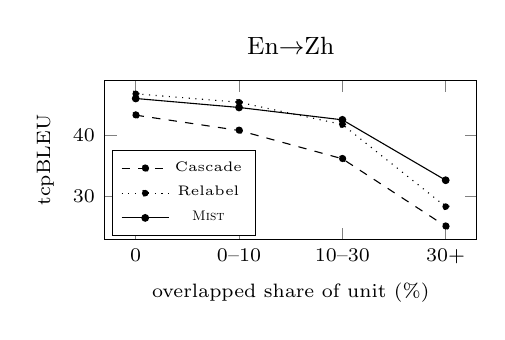
\begin{tikzpicture}\begin{axis}[width=0.52\columnwidth,height=3.6cm,xtick={0,1,2,3},
xticklabels={0,0--10,10--30,30+},xlabel={overlapped share of unit (\%)},ylabel={tcpBLEU},title={En$\rightarrow$Zh},
title style={font=\small},label style={font=\scriptsize},tick label style={font=\scriptsize},legend style={font=\tiny,at={(0.02,0.02)},anchor=south west}]
\addplot[dashed,mark=*,mark size=1.2pt] coordinates {(0,43.36) (1,40.84) (2,36.17) (3,25.04)}; \addlegendentry{Cascade}
\addplot[dotted,mark=*,mark size=1.2pt] coordinates {(0,46.88) (1,45.49) (2,41.82) (3,28.28)}; \addlegendentry{Relabel}
\addplot[solid,mark=*,mark size=1.2pt] coordinates {(0,46.11) (1,44.63) (2,42.59) (3,32.63)}; \addlegendentry{\sys{}}
\end{axis}\end{tikzpicture}
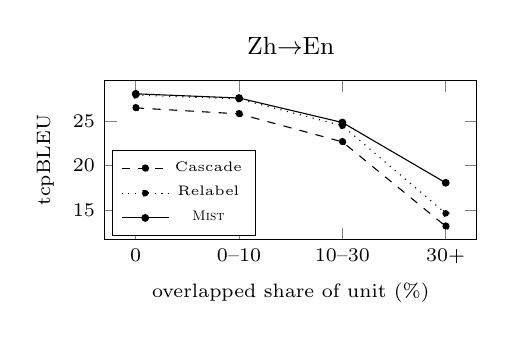
\begin{tikzpicture}\begin{axis}[width=0.52\columnwidth,height=3.6cm,xtick={0,1,2,3},
xticklabels={0,0--10,10--30,30+},xlabel={overlapped share of unit (\%)},ylabel={tcpBLEU},title={Zh$\rightarrow$En},
title style={font=\small},label style={font=\scriptsize},tick label style={font=\scriptsize},legend style={font=\tiny,at={(0.02,0.02)},anchor=south west}]
\addplot[dashed,mark=*,mark size=1.2pt] coordinates {(0,26.48) (1,25.81) (2,22.67) (3,13.19)}; \addlegendentry{Cascade}
\addplot[dotted,mark=*,mark size=1.2pt] coordinates {(0,27.91) (1,27.48) (2,24.48) (3,14.64)}; \addlegendentry{Relabel}
\addplot[solid,mark=*,mark size=1.2pt] coordinates {(0,28.06) (1,27.59) (2,24.84) (3,18.07)}; \addlegendentry{\sys{}}
\end{axis}\end{tikzpicture}
\caption{tcpBLEU by how much of a reference unit overlaps another speaker (reference windows, offline systems). The gap
between \sys{} and post-hoc relabelling opens where speakers overlap.}
\label{fig:overlap8}
\end{figure}


\paragraph{Labels or translation?} Relabelling \sys{}'s own output with the diarizer, keeping its text, separates the
two (re-review M09): on overlapped units its own labels score \num{v8:ov:en2zh:O2:ov} against
\num{v8:ov:en2zh:O2-relabel:ov} with diarizer labels (Zh$\rightarrow$En \num{v8:ov:zh2en:O2:ov} vs.\
\num{v8:ov:zh2en:O2-relabel:ov}), while with diarizer labels on both sides its text leads the speaker-blind model's by
\num{v8:ov:en2zh:O2-relabel:ov} vs.\ \num{v8:ov:en2zh:O2-nosd-relabel:ov}. Decoder-side speaker conditioning therefore mainly yields better
attributed segments under overlap: relabelling \sys{}'s own text costs \num{v8:ov:en2zh:O2:ov}$\rightarrow$\num{v8:ov:en2zh:O2-relabel:ov},
while its text with diarizer labels is only \num{v8:ov:en2zh:O2-relabel:ov} vs.\ \num{v8:ov:en2zh:O2-nosd-relabel:ov} for the
speaker-blind text; we do not claim that it translates overlapped speech better.

\paragraph{Short-turn fallback (C2).} For every window, a cascade segment of at most 1.5\,s is added to \sys{}'s output
when no \sys{} segment of the same diarizer slot overlaps it within 0.5\,s and no nearby \sys{} text has chrF $\ge$50 with
it. On offline \sys{} this raises tcpBLEU in all three sets (Table~\ref{tab:overlap8}) and concurrent-speaker recall to
\num{v8:ov:en2zh:C2_O:cr} / \num{v8:ov:zh2en:C2_O:cr} / \num{v8:ov:ali:C2_O:cr}\%; on \sys{}-Simul it raises recall but
lowers tcpBLEU slightly, so by the pre-registered criterion it is adopted only for the offline model.

\paragraph{Latency.} Table~\ref{tab:lat8} queues the reads of a meeting on one decoder stream at the median single-stream
read time measured in v6 (batch 1, two H200 cards, HuggingFace eager decoding). The wall-clock replay (B6) could only run beside another
training job that held about \num{v8:b6:foreign_gib}\,GiB and most of the compute of every card (prereg\_v8 amendments 3--4),
with the Thinker spread over three cards at batch 1, so its real-time factor is an upper bound on the single-stream one.
On the one meeting completed (AliMeeting \num{v8:b6:ali_S2dl:meeting}, \sys{}-Simul) the median read took
\num{v8:b6:ali_S2dl:readp50}\,ms, \num{v8:b6:ali_S2dl:over}\% of the reads exceeded the 1\,s cadence, and the measured
real-time factor is \num{v8:b6:ali_S2dl:rtf}. By the pre-registered rule this is inconclusive, not a negative result:
contention only slows reads down, and an upper bound above 1 says nothing about the uncontended case. The user then
stopped the remaining B6 runs, since further contended runs could not change that conclusion; two runs stopped part-way
(En$\rightarrow$Zh \sys{}-Simul, \num{v8:b6:en2zh_S2dl:done} of \num{v8:b6:en2zh_S2dl:of} windows; AliMeeting LocalAgreement,
\num{v8:b6:ali_O2_LA2:done} of \num{v8:b6:ali_O2_LA2:of}) are not used. The real-time factors of Table~\ref{tab:lat8} remain
estimates from the measured single-stream read time, not a replay. LocalAgreement's reads take longer than the 1\,s read period, so queued it falls
behind without bound (per-speaker median \num{v8:lat:en2zh:O2_LA2:ps:p50}\,s). OpenSTBench-style start offset and
average delay of \sys{}-Simul (per-speaker channels, units spread uniformly over their block): \num{v8:lat:en2zh:S2dl:ps:start} and
\num{v8:lat:en2zh:S2dl:ps:atd}\,s in En$\rightarrow$Zh; these are not comparable with numbers reported on single-speaker
clips. Streams of more than 400 blocks (runaway repetition) were not synthesised: \num{v8:lat:ali:S2dl:ps:cens} on
AliMeeting, none elsewhere; counted as never heard, they leave the percentiles unchanged at the reported precision.

\paragraph{Fixed lag and seeds.} On the 8 AMI meetings of the v7 subset (prereg\_v8 amendment 2), fixed lag 2\,s on the
prefix-trained model scores \num{v8:sub:en2zh:lag2:all} tcpBLEU against \sys{}-Simul's \num{v8:sub:en2zh:on_S2dl:all} and
LocalAgreement's \num{v8:sub:en2zh:pla2:all} (En$\rightarrow$Zh; Zh$\rightarrow$En \num{v8:sub:zh2en:lag2:all} /
\num{v8:sub:zh2en:on_S2dl:all} / \num{v8:sub:zh2en:pla2:all}), but on overlapped units \num{v8:sub:en2zh:lag2:ov} vs.\
\num{v8:sub:en2zh:on_S2dl:ov} (\num{v8:sub:zh2en:lag2:ov} vs.\ \num{v8:sub:zh2en:on_S2dl:ov}), with a median text lag on
overlapped units of \num{v8:sub:en2zh:lag2:lagov} vs.\ \num{v8:sub:en2zh:on_S2dl:lagov}\,s. On the 10 AliMeeting subset
meetings (completed after the other runs, prereg\_v8 amendment 3, exploratory) fixed lag is ahead of \sys{}-Simul overall
and on overlapped units (\num{v8:sub:ali:lag2:all} / \num{v8:sub:ali:lag2:ov} vs.\ \num{v8:sub:ali:on_S2dl:all} /
\num{v8:sub:ali:on_S2dl:ov}; LocalAgreement \num{v8:sub:ali:pla2:all} / \num{v8:sub:ali:pla2:ov}), again at a longer lag on
overlapped units (\num{v8:sub:ali:lag2:lagov} vs.\ \num{v8:sub:ali:on_S2dl:lagov}\,s). Whole-meeting tcpBLEU of
\sys{}-Simul over training seeds: \num{v8:seed:en2zh:all} (En$\rightarrow$Zh, \num{v8:seed:en2zh:n} seeds; overlapped
\num{v8:seed:en2zh:ov}), \num{v8:seed:zh2en:all} (Zh$\rightarrow$En, \num{v8:seed:zh2en:n}), \num{v8:seed:ali:all}
(AliMeeting, \num{v8:seed:ali:n}).

\paragraph{Playback scheduling.} Table~\ref{tab:sched8} replays \sys{}-Simul's committed blocks under four single-channel
policies and the per-speaker layout. Captions for short overlapped interjections and skipping stale blocks bound the lag
of what is spoken, but on AliMeeting, where speakers overlap most, only \num{v8:b7:ali:d:cov}\% of the units are then
spoken.

\begin{table*}[t]
\centering\small
\begin{tabular}{lrrrrrrrrr}
\toprule
 & \multicolumn{3}{c}{En$\rightarrow$Zh} & \multicolumn{3}{c}{Zh$\rightarrow$En} & \multicolumn{3}{c}{AliMeeting} \\
\cmidrule(lr){2-4}\cmidrule(lr){5-7}\cmidrule(lr){8-10}
Playback & p50 & p90 & spoken & p50 & p90 & spoken & p50 & p90 & spoken \\
\midrule
one channel, as is & 142.4 & 772.6 & 100 & 26.4 & 313.0 & 100 & 604.6 & 2481.2 & 100 \\
short interjections as captions & 43.9 & 320.6 & 91 & 13.3 & 47.5 & 94 & 441.0 & 1630.3 & 93 \\
skip blocks $>$10\,s late & 9.7 & 11.8 & 80 & 9.8 & 13.1 & 82 & 10.8 & 17.2 & 35 \\
b + c & 9.1 & 11.6 & 80 & 9.4 & 12.9 & 82 & 10.8 & 17.4 & 35 \\
one channel per speaker, mixed & 7.4 & 12.2 & 100 & 8.2 & 15.1 & 100 & 23.2 & 314.1 & 100 \\
\bottomrule
\end{tabular}
\caption{Playback scheduling of \sys{}-Simul's whole-meeting output (reads queued; nothing re-synthesised, so the speech
of every played block is unchanged): listener completion lag (s) of the units played, and the share of units spoken
(\%; the rest are shown as captions). prereg\_v8 amendment 1.}
\label{tab:sched8}
\end{table*}


\paragraph{Voice prompts (B8).} On the 8 whole AMI En$\rightarrow$Zh meetings of v7's second half (3{,}318 output
streams), the Talker was run again with only the most recent 1\,s of a slot heard alone as its prompt instead of up to
8\,s, nothing else changed. The short prompt makes the voices less like the attributed speaker (WavLM SIM
\num{v8:b8:1s:sim} vs.\ \num{v8:b8:8s:sim}, meeting-bootstrap intervals \num{v8:b8:1s:simci} and \num{v8:b8:8s:simci}),
more often closer to another speaker of the window (\num{v8:b8:1s:conf} vs.\ \num{v8:b8:8s:conf}\%) and slightly less
intelligible (ASR-BLEU against the Talker's input \num{v8:b8:1s:asr} vs.\ \num{v8:b8:8s:asr}), so we keep 8\,s. At the
first commit \num{v8:b8:avail1}\% of the streams have 1\,s heard alone and \num{v8:b8:avail8}\% a full 8\,s. Holding a
slot's speech until 1\,s of it has been heard alone, instead of starting with the fallback prompt, would delay
\num{v8:b8:wait:streams}\% of the streams (\num{v8:b8:wait:blocks}\% of the blocks), but those by a median
\num{v8:b8:wait:p50}\,s (90th percentile \num{v8:b8:wait:p90}\,s): slots that rarely talk alone. Speaking at once is the
better default.

\paragraph{Threshold flips (B5).} The causality check (Appendix~\ref{app:causal}) found \num{v8:b5:frames} distinct
80\,ms frames whose 0.5 activity decision differs between the prefix run and the dump. Rebuilding the online windows
with the prefix values changes \num{v8:b5:bound_same} window boundaries (none moves). The \num{v8:b5:windows} windows
holding a flipped frame were decoded again, each together with a copy using the original posteriors in the same batch:
\num{v8:b5:flip_same} are token-identical; an unchanged copy decoded in the same batch is identical in
\num{v8:b5:dup_same}. With so few windows the two cannot be told apart: the flips change outputs no more than
re-decoding does, but this check cannot show that they change nothing.

\paragraph{Full-coverage references.} The reference windows keep \num{v6:filt:en2zh:all:dur}\% of the En$\rightarrow$Zh
test speech. Every test utterance has a selected translation (Appendix~\ref{app:data}), so we also score the whole-meeting
runs on all \num{v8:full:en2zh:on_S2dl:units} non-hesitation units: \sys{}-Simul \num{v8:full:en2zh:on_S2dl:all}, LocalAgreement
on the offline model \num{v8:full:en2zh:on_O2_LA2:all}; overlapped units \num{v8:full:en2zh:on_S2dl:ov} vs.\
\num{v8:full:en2zh:on_O2_LA2:ov}. These are still machine translations.



\end{document}
